% !TEX program = xelatex
\documentclass[UTF8]{ctexart}

\RequirePackage{amsmath}
\RequirePackage{chemfig}
\RequirePackage{mhchem}
\RequirePackage{graphicx}

\RequirePackage{inputenc}
\RequirePackage{fontspec}
\RequirePackage{xeCJK}

\RequirePackage{ruby}

\setmainfont{Times New Roman}

\setCJKmainfont{等线}
\setCJKsansfont{等线}
\setCJKmonofont{等线}

\usepackage{geometry}
\geometry
{
    left=1.25in,
    right=1.25in,
    top=1in,
    bottom=1in
}

\title{生物笔记}
\author{李宇轩}
\date{2019.07.29}

\begin{document}

\maketitle

\newpage

\tableofcontents

\newpage

\setlength{\parindent}{0pt}

\section{生命的物质基础}

\subsection{水}
    自由水:以游离态存在,可以自由流动。\\[3mm]
    结合水:与细胞内其他物质结合。\\[3mm]
    在人体中,水约占体重的$70\%$,当缺水$10\%$时,生理活动紊乱,当缺水$20\%$时,生命活动终止。

\subsection{无机盐}
    生物体内的无机盐大多数以离子形态存在。\\[3mm]
    以下列举了无机盐在组成生物体结构中的作用:\vspace{5pt}
    \begin{table}[h]
        \begin{center}
            \begin{tabular}{l|l}
                \hline
                \ce{Ca^{2+}}\qquad\qquad&构成骨骼和牙齿的重要成分\qquad\qquad\\ \hline
                \ce{Fe^{2+}}\qquad\qquad&合成血红蛋白的重要成分\qquad\qquad\\ \hline
                \ce{Mg^{2+}}\qquad\qquad&合成叶绿素的重要成分\qquad\qquad\\ \hline
            \end{tabular}
            \caption{无机盐在组成生物体结构中的作用}
        \end{center}
    \end{table}\\
    以下列举了无机盐在调节生物体代谢活动中的作用:\vspace{5pt}
    \begin{table}[h]
        \begin{center}
            \begin{tabular}{l|l}
                \hline
                \ce{CO3^{2-}}\qquad\qquad&中和血液中的碱性物质\qquad\qquad\\ \hline
                \ce{HCO3^{-}}\qquad\qquad&中和血液中的酸性物质\qquad\qquad\\ \hline
                \ce{Ca^{2+}}\qquad\qquad&含量过低会导致肌肉抽搐\qquad\qquad\\ \hline
                \ce{K+}\qquad\qquad&用于神经细胞传递电信号,静息电位时主要处于膜内\qquad\qquad\\ \hline
                \ce{Na+}\qquad\qquad&用于神经细胞传递电信号,静息电位时主要处于膜外\qquad\qquad\\ \hline
            \end{tabular}
            \caption{无机盐在调节生物体代谢活动中的作用}
        \end{center}
    \end{table}\\
    以下列举了无机盐缺少对植物叶片生长的影响:\vspace{5pt}
    \begin{table}[h]
        \begin{center}
            \begin{tabular}{l|l}
                \hline
                \ce{Mg^{2+}}\qquad\qquad&叶脉缺绿,叶片变黄变白\qquad\qquad\\ \hline
                \ce{Mn^{2+}}\qquad\qquad&叶脉间缺绿,叶片坏死\qquad\qquad\\ \hline
                \ce{Zn^{2+}}\qquad\qquad&叶片边缘撕裂萎缩,幼叶和茎生长受到抑制\qquad\qquad\\ \hline
            \end{tabular}
            \caption{无机盐缺少对植物叶片生长的影响}
        \end{center}
    \end{table}

\newpage

\subsection{糖类}
    我们将符合化学通式~~\ce{(CH2O)_n}~的物质称为糖类,俗称碳水化合物。

\subsubsection{单糖}
    单糖:葡萄糖,果糖,核糖\\[2mm]
    单糖指的是最简单的不能水解的糖类。\vspace{10pt}
    \begin{table}[h]
        \begin{center}
            \begin{tabular}{l|l}
                \hline
                葡萄糖\qquad\qquad&存在于动植物细胞中,属于六碳糖\qquad\qquad\\ \hline
                果糖\qquad\qquad&存在于蜂蜜和水果中,属于六碳糖\qquad\qquad\\ \hline
                核糖\qquad\qquad&构成核酸的重要成分,属于五碳糖\\ \hline
            \end{tabular}
            \caption{单糖的分类}
        \end{center}
    \end{table}\vspace{-5pt}

\subsubsection{双糖}
    双糖:蔗糖,乳糖,麦芽糖\\[2mm]
    双糖指的是由两个单糖脱水缩合形成的糖类。\vspace{10pt}
    \begin{table}[h]
        \begin{center}
            \begin{tabular}{l|l}
                \hline
                蔗糖\qquad\qquad&存在于甘蔗和甜菜中,易溶于水,由一份葡萄糖和一份果糖组成\qquad\qquad\\ \hline
                乳糖\qquad\qquad&存在于动物的乳汁中,易溶于水,由一份葡萄糖和一份半乳糖组成\qquad\qquad\\ \hline
                麦芽糖\qquad\qquad&存在于发芽的小麦种子中,易溶于水,由两份葡萄糖组成\\ \hline
            \end{tabular}
            \caption{双糖的分类}
        \end{center}
    \end{table}\vspace{-5pt}

\subsubsection{多糖}
    多糖:淀粉,糖原,纤维素\\[2mm]
    多糖指的是由多个单糖脱水缩合形成的糖类。\vspace{10pt}
    \begin{table}[h]
        \begin{center}
            \begin{tabular}{l|l}
                \hline
                淀粉\qquad\qquad&植物体内存储糖类的形式,不溶于水,由多份葡萄糖组成\qquad\qquad\\ \hline
                糖原\qquad\qquad&动物体内存储糖类的形式,不溶于水,由多份葡萄糖组成\qquad\qquad\\ \hline
                纤维素\qquad\qquad&组成植物细胞壁的主要成分,不溶于水,由多份葡萄糖组成\\ \hline
            \end{tabular}
            \caption{多糖的分类}
        \end{center}
    \end{table}\\
多糖和脂质结合称为糖指。\\[3mm]
多糖和蛋白质结合称为糖蛋白。

\subsection{脂质}
    我们将不溶于水而易溶于有机溶剂的物质称为脂质。

\subsubsection{脂肪}
    脂肪由甘油和三条脂肪酸组成。\\[3mm]
    若三条脂肪酸中均为碳碳单键(\chemfig{C-C}),称为饱和脂肪酸。\\[3mm]
    若三条脂肪酸中存在碳碳双键(\chemfig{C=C}),称为不饱和脂肪酸。\\[3mm]
    植物油常温下呈液态,是由于其脂肪酸分子存在不饱和脂肪酸,熔点较高,常温下不易凝结。\\[3mm]
    动物油常温下呈固态,是由于其脂肪酸分子均属于饱和脂肪酸,熔点较低,常温下容易凝结。

\subsubsection{磷脂}
    磷脂由亲水头部和疏水尾部组成。\\[3mm]
    亲水头部:由含氮碱基和磷酸和甘油组成。\\[3mm]
    疏水尾部:由两条脂肪酸组成。\\[3mm]
    磷脂可以构成磷脂单分子层,外部亲水,内部亲油,该结构存在于脂蛋白中。\\[3mm]
    磷脂可以构成磷脂双分子层,外部亲水,内部亲水,该结构存在于细胞膜中。
    \begin{figure}[h]
        \begin{center}
            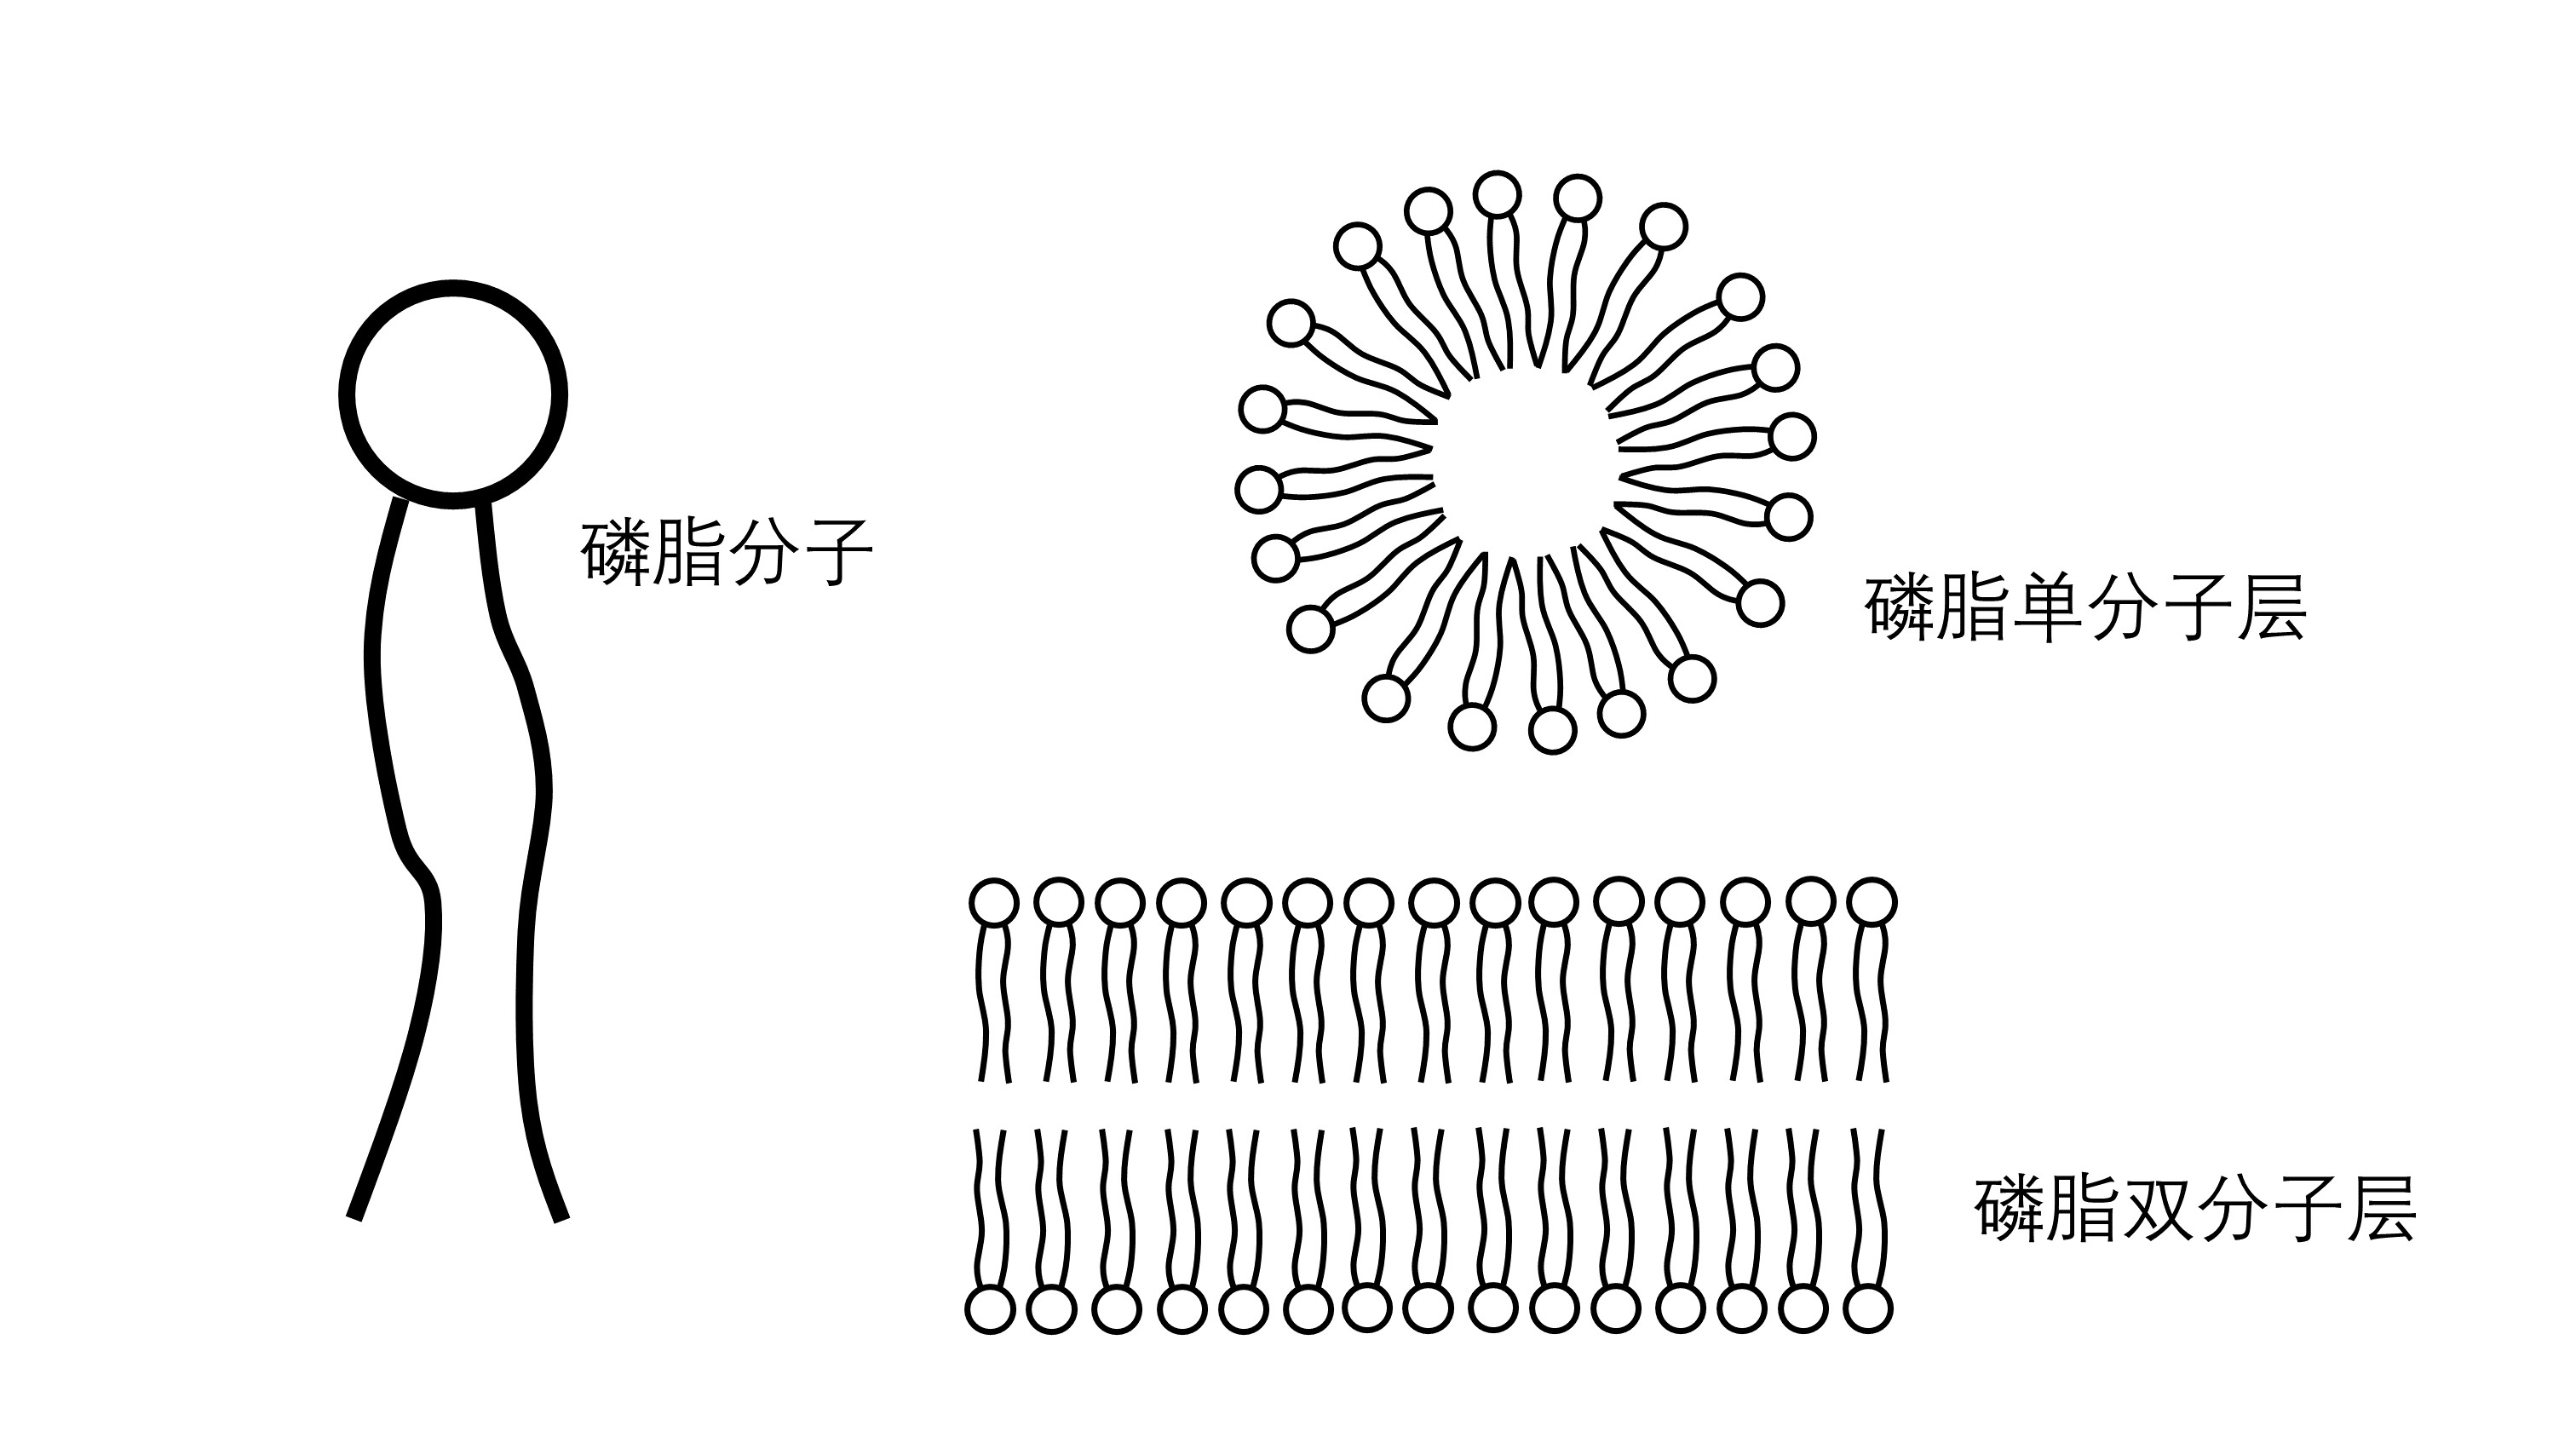
\includegraphics[width=10cm]{BiologyImage/1.jpg}    
            \caption{磷脂示意图}
        \end{center}
    \end{figure}

\subsubsection{胆固醇}
    胆固醇是组成细胞膜的重要成分,人体中主要分布在神经组织和内脏组织中。\\[3mm]
    胆固醇参与合成的物质:维生素D,雄激素,雌激素,肾上腺皮质激素。

\newpage

\subsection{蛋白质}
    蛋白质是由氨基酸为单体组成的大分子化合物。\\[3mm]
    蛋白质的元素组成:\ce{C},\ce{H},\ce{O},\ce{N},\ce{S}\\[6mm]
    氨基酸的结构上的特点:同一个碳上接有一个氢~\ce{H},一个羧基~\ce{NH2},一个氨基~\ce{COOH}。\\[3mm]
    氨基酸的结构上的差异:同一个碳上侧链所连接的基团\ce{R},对于每一种氨基酸可以各不相同。\\[3mm]
    氨基酸的结构式:
    \begin{figure}[h]
        \begin{center}
            \chemfig
            {
                NH_{2}-[0,0.7]
                C(-[2,0.7]H)(-[-2,0.7]R)-[0,0.7]COOH
            }
            \caption{氨基酸的结构式}
        \end{center}
    \end{figure}\\
    氨基酸的脱水缩合过程:两个氨基酸,一个在羧基上脱去一个羟基,一个在氨基上脱去一个氢,两者结合形成了肽键,生成二肽,同时释放出一份水。\\[3mm]
    肽键的结构式:\\
    \begin{figure}[h]
        \begin{center}
            \chemfig{-[0,0.7]C(=[2,0.7]O)-[0,0.7]N(-[2,0.7]H)-[0,0.7]}        
            \caption{肽键的结构式}
        \end{center}
    \end{figure}\\
    氨基酸间的键称为肽键,氨基酸连接的产物称为肽链。\\[3mm]
    通常我们将三个以上的氨基酸组成的肽链称为多肽。\\[8mm]
    蛋白质是肽链经过折叠和螺旋而形成的,蛋白质具有一定的空间结构。\\[3mm]
    蛋白质的多样性:氨基酸的数目,氨基酸的种类,氨基酸的排列,蛋白质的折叠方式。

\newpage
    

\subsection{核酸}
    核酸是由核苷酸为单体组成的大分子化合物。\\[3mm]
    核酸的元素组成:\ce{C},\ce{H},\ce{O},\ce{N},\ce{P}\\[6mm]
    以下表格列举了核苷和核苷酸的差异:\vspace{5pt}
    \begin{table}[h]
        \begin{center}
            \begin{tabular}{l|l}
                \hline
                核苷\qquad\qquad&一个含氮碱基,一个五碳糖\qquad\qquad\\ \hline
                核苷酸\qquad\qquad&一个含氮碱基,一个五碳糖,一个磷酸\qquad\qquad\\ \hline
            \end{tabular}
            \caption{核苷和核苷酸的差异}
        \end{center}
    \end{table}\\
    以下图片展示了核苷和核苷酸的差异:
    \begin{figure}[h]
        \begin{center}
            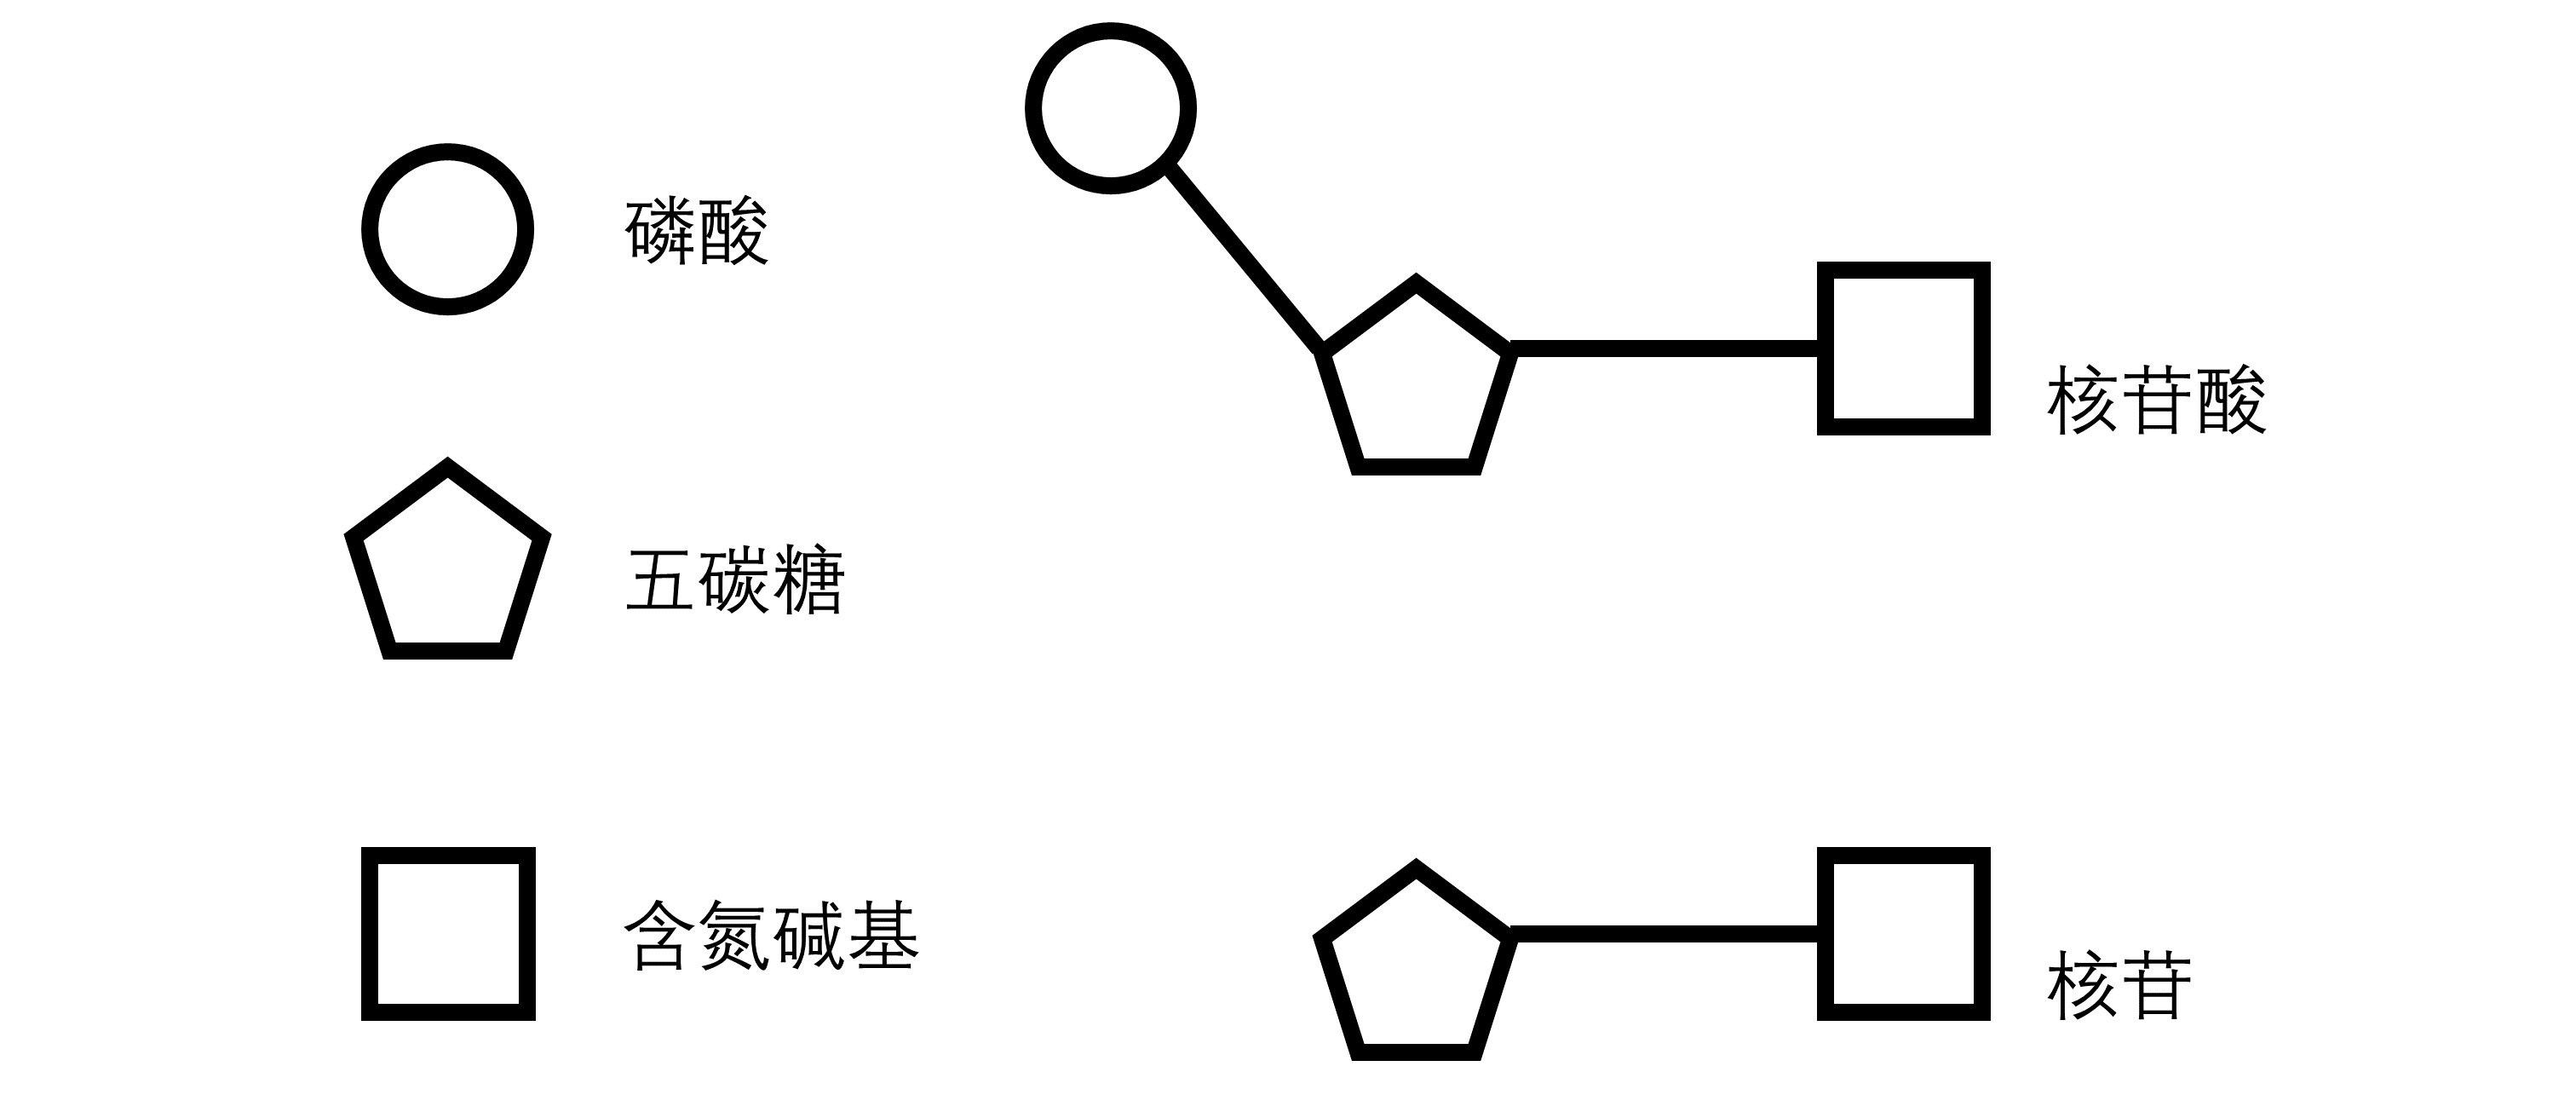
\includegraphics[width=10cm]{BiologyImage/2.jpg}
            \caption{核苷和核苷酸的差异}
        \end{center}
    \end{figure}\\
    核苷可以具体分为两种:脱氧核苷,核糖核苷。\\[3mm]
    核苷酸可以具体分为两种:脱氧核苷酸,核糖核苷酸。\\[3mm]
    以下表格列举了脱氧核苷酸和核糖核苷酸的差异:\vspace{5pt}
    \begin{table}[h]
        \begin{center}
            \begin{tabular}{l|l|l|l|l|l}
                \hline
                类型\qquad\qquad&五碳糖&含氮碱基1&含氮碱基2&含氮碱基3&含氮碱基4\\ \hline
                核糖核苷酸~~~~&核糖&U-尿嘧啶&C-胞嘧啶&G-鸟嘌呤&A-腺嘌呤\\ \hline
                脱氧核苷酸~~~~&脱氧核糖&T\,-胸腺嘧啶&C-胞嘧啶&G-鸟嘌呤&A-腺嘌呤\\ \hline
            \end{tabular}
            \caption{脱氧核苷酸和核糖核苷酸的差异}
        \end{center}
    \end{table}\\
    核酸是由核苷酸构成的物质。\\[3mm]
    DNA是由脱氧核苷酸构成的核酸,主要存在于细胞核中,全称脱氧核糖核酸。\\[3mm]
    RNA是由核糖核苷酸构成的核酸,主要存在于细胞质中,全称核糖核酸。\\[3mm]

\newpage

\subsection{维生素}
    维生素是生物的生长和代谢所必须的微量有机化合物。\\[3mm]
    维生素并不是某种特定类型的物质,符合上述要求的物质均可以称为维生素。\\[3mm]
    以下表格列举了部分维生素的作用:\vspace{5pt}
    \begin{table}[h]
        \begin{center}
            \begin{tabular}{l|l|l}
                \hline
                维生素A\qquad\qquad&脂溶性维生素\qquad\qquad&夜盲症\qquad\qquad\\ \hline
                维生素B$_1$\qquad\qquad&水溶性维生素\qquad\qquad&脚气病\qquad\qquad\\ \hline
                维生素B$_2$\qquad\qquad&水溶性维生素\qquad\qquad&口腔溃疡\qquad\qquad\\ \hline
                维生素C\qquad\qquad&水溶性维生素\qquad\qquad&坏血病\qquad\qquad\\ \hline
                维生素D\qquad\qquad&脂溶性维生素\qquad\qquad&佝偻病\qquad\qquad\\ \hline
            \end{tabular}
            \caption{维生素的作用}
        \end{center}
    \end{table}

\subsection{营养物质的能量}
    以下表格列举了营养物质氧化分解产生的能量:\vspace{5pt}
    \begin{table}[h]
        \begin{center}
            \begin{tabular}{l|l}
                \hline
                营养物质\qquad\qquad&氧化分解能量\qquad\qquad\\ \hline
                糖类&$16.4$kJ\\ \hline
                脂质&$37.6$kJ\\ \hline
                蛋白质&$16.7$kJ\\ \hline
            \end{tabular}
        \end{center}
    \end{table}

\subsection{营养物质的检测}
    以下表格列举了营养物质的检测方法:\vspace{5pt}
    \begin{table}[h]
        \begin{center}
            \begin{tabular}{l|l|l|l}
                \hline
                营养物质\qquad\qquad&所用试剂\qquad\qquad\qquad&实验操作\qquad\qquad&实验现象\qquad\qquad\\ \hline
                糖类&班氏试剂&加热&溶液由蓝色变为红色\\ \hline
                蛋白质&双缩脲试剂&振荡&溶液由蓝色变为紫色\\ \hline
                脂肪&苏丹Ⅲ染液&振荡&溶液由红色变为橘黄色\\ \hline
            \end{tabular}
            \caption{营养物质的检测}
        \end{center}
    \end{table}\\
    1.表中的糖类检测方法只能检测还原性糖,包含葡萄糖,果糖,乳糖,麦芽糖。\\[3mm]
    2.表中的双缩脲试剂由氢氧化钠和硫酸铜组成,实验时应当先加入氢氧化钠再加入硫酸铜。

\section{生命的结构基础}

\subsection{细胞膜}
    细胞膜主要由磷脂分子和蛋白质分子构成,
    细胞膜具有半流动性。\\[3mm]
    细胞膜的外侧有少量多糖分子,
    附着在磷脂上的被称为糖脂,
    附着在蛋白质上的被称为糖蛋白。
    其中细胞膜上的糖蛋白具有信号识别的作用,
    可以帮助细胞识别外界信息。\\[3mm]
    细胞膜的功能特点:保护细胞,物质交换,信息交流。

\subsubsection{自由扩散}
    自由扩散顺浓度阶梯进行,不需要能量。\\[3mm]
    自由扩散主要用于通过一些脂溶性有机物和一些无机分子:\ce{O2},\ce{CO2},\ce{H2O},甘油,尿素

\subsubsection{协助扩散}
    协助扩散顺浓度阶梯进行,不需要能量。\\[3mm]
    协助扩散过程中,需要载体蛋白协助。\\[3mm]
    协助扩散主要用于通过一些水溶性无机物和一些无机离子:\ce{Na+},\ce{Cl-},葡萄糖,氨基酸,核苷酸

\subsubsection{主动运输}
    主动运输逆浓度阶梯进行,需要能量。\\[3mm]
    主动运输过程中,需要载体蛋白协助。\\[3mm]
    主动运输通常是运输无机离子,例如神经细胞中~\ce{Na+}和~\ce{K+}的运输,例如海藻细胞中~\ce{I-}的摄取。

\subsubsection{胞吞和胞吐}
    胞吞和胞吐通过细胞膜的变形运输物质,需要能量。\\[3mm]
    胞吞和胞吐通常用于运输大分子或颗粒物,例如白细胞吞噬病毒,例如胰岛细胞释放胰岛素。\vspace{15pt}
    \begin{figure}[h]
        \begin{center}
            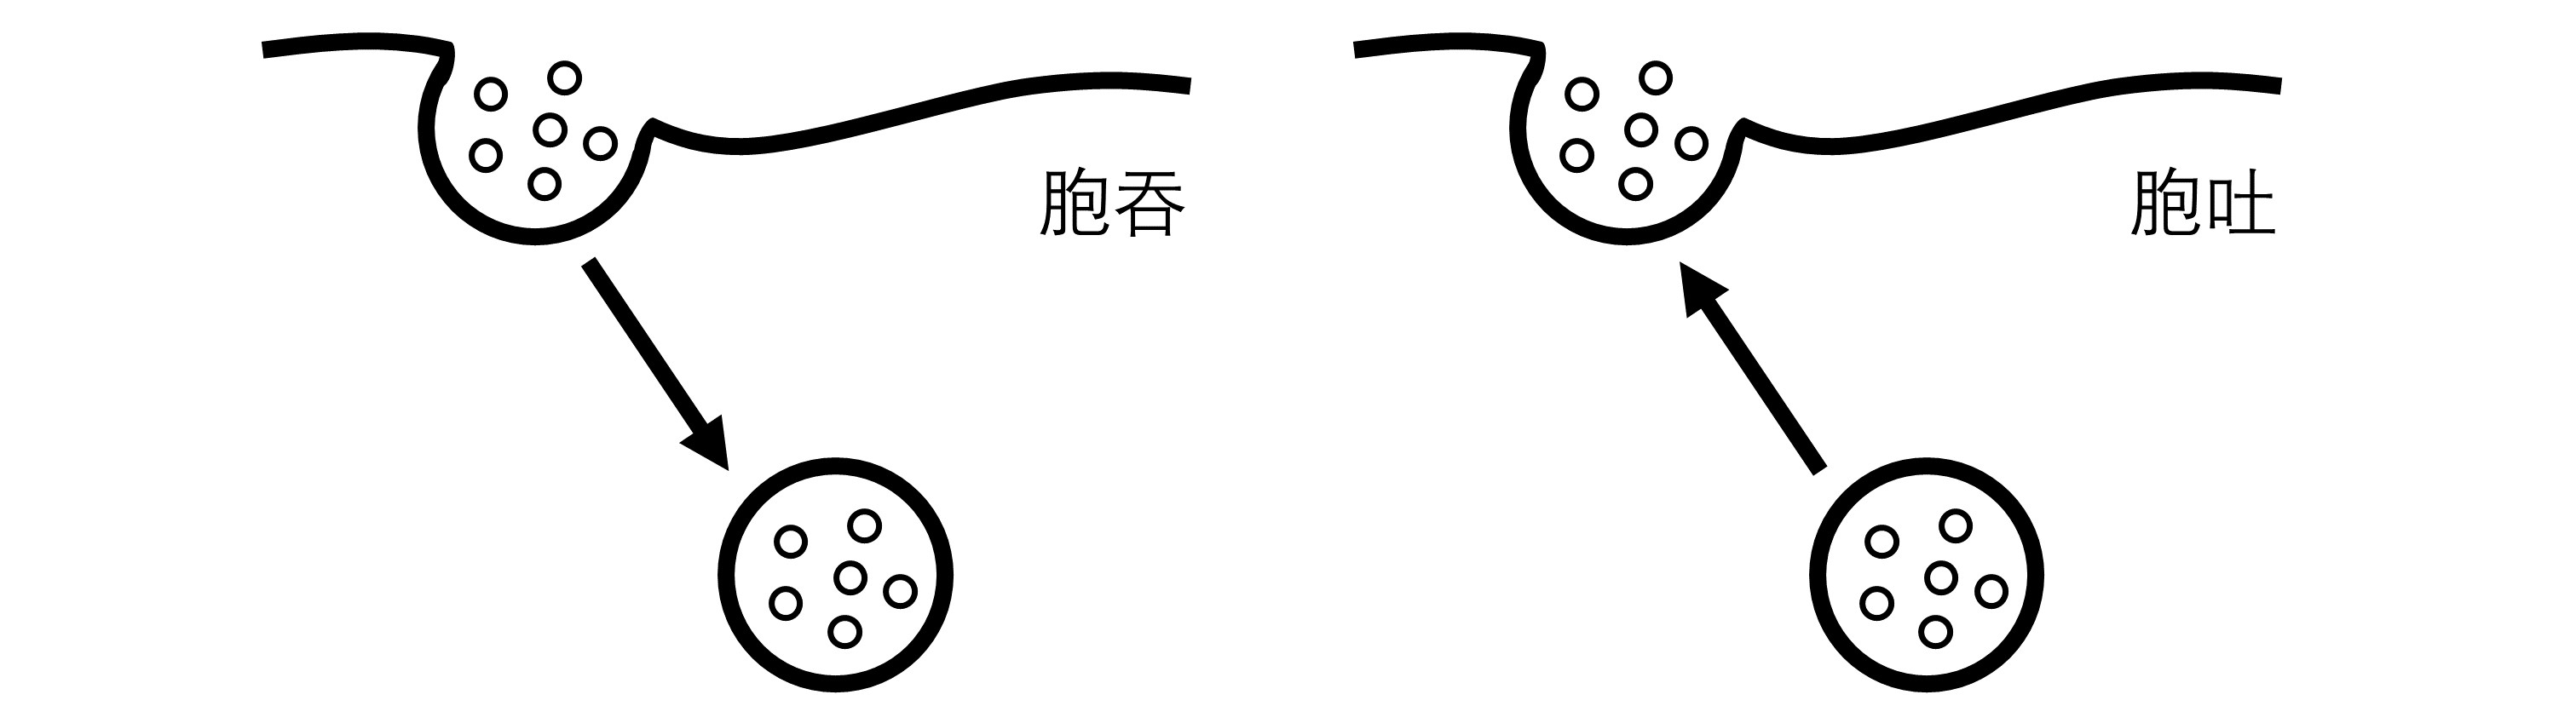
\includegraphics[width=10cm]{BiologyImage/3.jpg}
            \caption{胞吞和胞吐}
       \end{center}
    \end{figure}


\newpage
    
    \subsubsection{细胞的吸水和失水}
    若外界离子浓度高于细胞液浓度,水分会由内向外渗出,细胞失水萎缩。\\[3mm]
    若外界离子浓度低于细胞液浓度,水分会由外向内渗入,细胞吸水膨胀。\\[3mm]
    植物细胞中,我们将细胞膜,细胞质,液泡膜合称为原生质层。
    当植物细胞浸入高浓度溶液时,由于失水导致原生质层萎缩,
    容易变形的细胞膜随之萎缩,不易变形的细胞壁则保持原有形状,
    因此我们会观察到细胞壁和细胞膜分离的现象,该现象被称为质壁分离。\\
    
\subsection{细胞核}
    细胞核指的是细胞中球形或椭球形的部分。\\[3mm]
    细胞核由以下部分组成:\vspace{5pt}
    \begin{table}[h]
        \begin{center}
            \begin{tabular}{l|l}
                \hline
                核膜\qquad\qquad&由两层膜组成,控制细胞核内外物质交换和信息传输\qquad\qquad\\ \hline
                核孔\qquad\qquad&细胞核膜上的许多小孔,是细胞核和细胞质间进行物质交换的通道\qquad\qquad\\ \hline
                核仁\qquad\qquad&细胞核内的的数个圆球形结构,与核糖体的形成有关\qquad\qquad\\ \hline
                核基质\qquad\qquad&细胞核内的基质,形态透明均匀,富含丰富的营养物质\qquad\qquad\\ \hline
                染色质\qquad\qquad&细胞核内的细丝状物质,可以被碱性染料染色\qquad\qquad\\ \hline
            \end{tabular}
            \caption{细胞核的结构组成}
        \end{center}
    \end{table}\\
    细胞核中对染色质进行染色时,通常使用的染料有苏木精,龙胆紫,醋酸洋红。\\[3mm]
    细胞核是储存遗传物质的场所,是细胞生长,发育,分裂增殖的调控中心。\\
    
\subsection{细胞质}
    细胞质指的是细胞核和细胞膜之间的物质。\\[3mm]
    细胞质由以下部分组成:\vspace{5pt}
    \begin{table}[h]
        \begin{center}
            \begin{tabular}{l|l}
                \hline
                细胞质基质\qquad\qquad&细胞质中的基质,富含丰富的营养物质\qquad\qquad\\ \hline
                细胞器\qquad\qquad&细胞质基质中具有特定功能的结构\qquad\qquad\\ \hline
            \end{tabular}
            \caption{细胞质的结构组成}
        \end{center}
    \end{table}\\
    细胞质基质呈液态,其中的营养物质和液体环境为细胞代谢提供了原料和反应场所。\\[3mm]
    细胞质基质是细胞代谢的基本场所。

\newpage

\subsubsection{核糖体}
    核糖体无膜结构。\\[2mm]
    核糖体是由蛋白质和核糖体RNA组成的微小颗粒,参与蛋白质的合成。\vspace{-10pt}
    \begin{figure}[h!]
        \begin{center}
            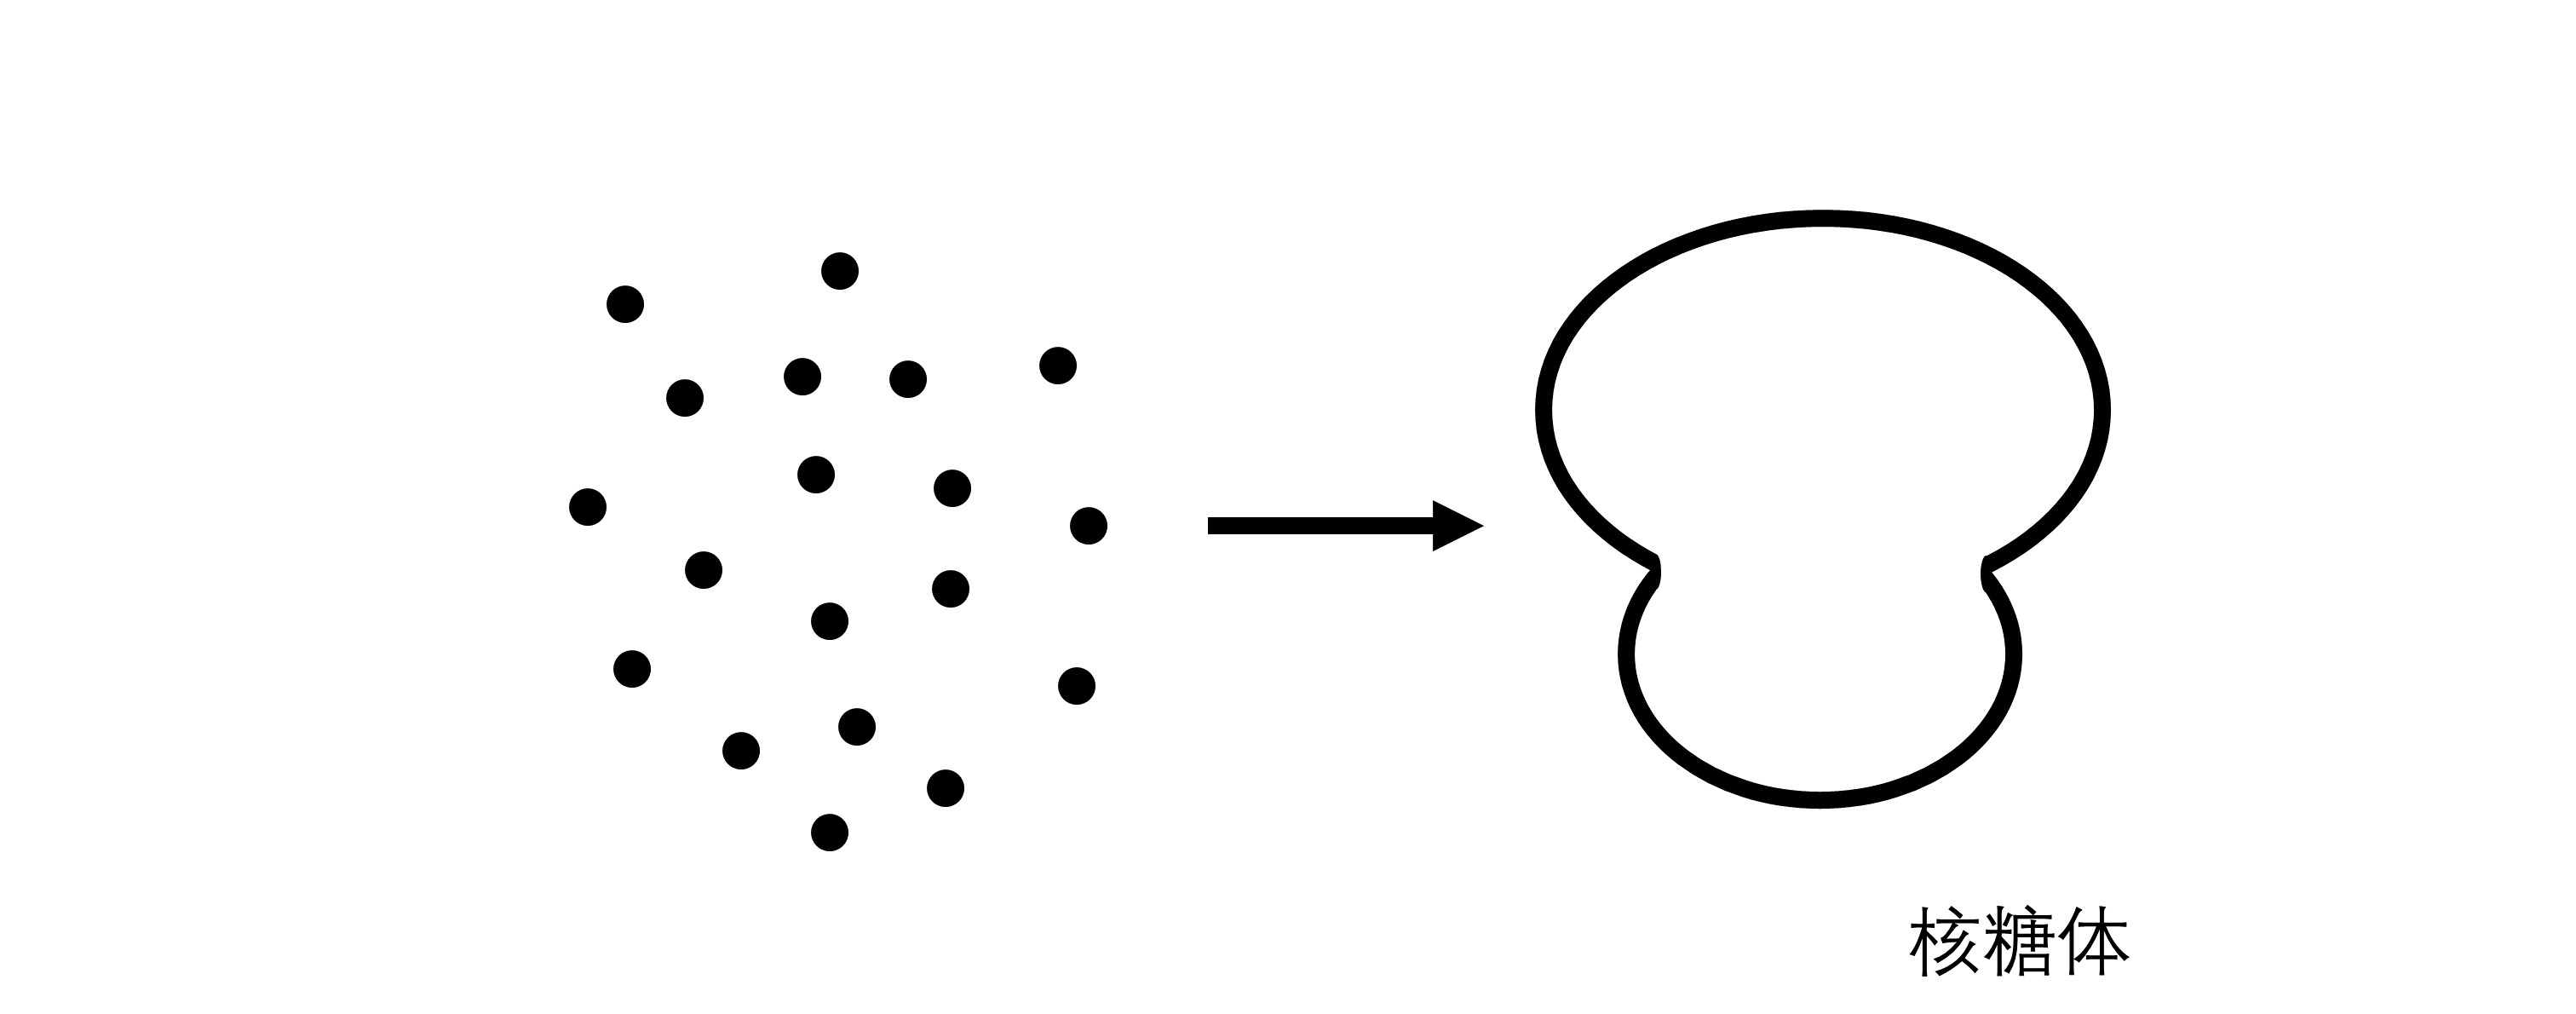
\includegraphics[width=9cm]{BiologyImage/4.jpg}
            \caption{核糖体结构示意图}
        \end{center}
    \end{figure}\vspace{-32.5pt}

\subsubsection{中心体}
    中心体无膜结构。\\[2mm]
    中心体是由两个互相垂直的中心粒和周围物质组成,与细胞的有丝分裂有关。\\[2mm]
    中心体仅存在于动物和部分低等植物。\vspace{-10pt}
    \begin{figure}[h!]
        \begin{center}
            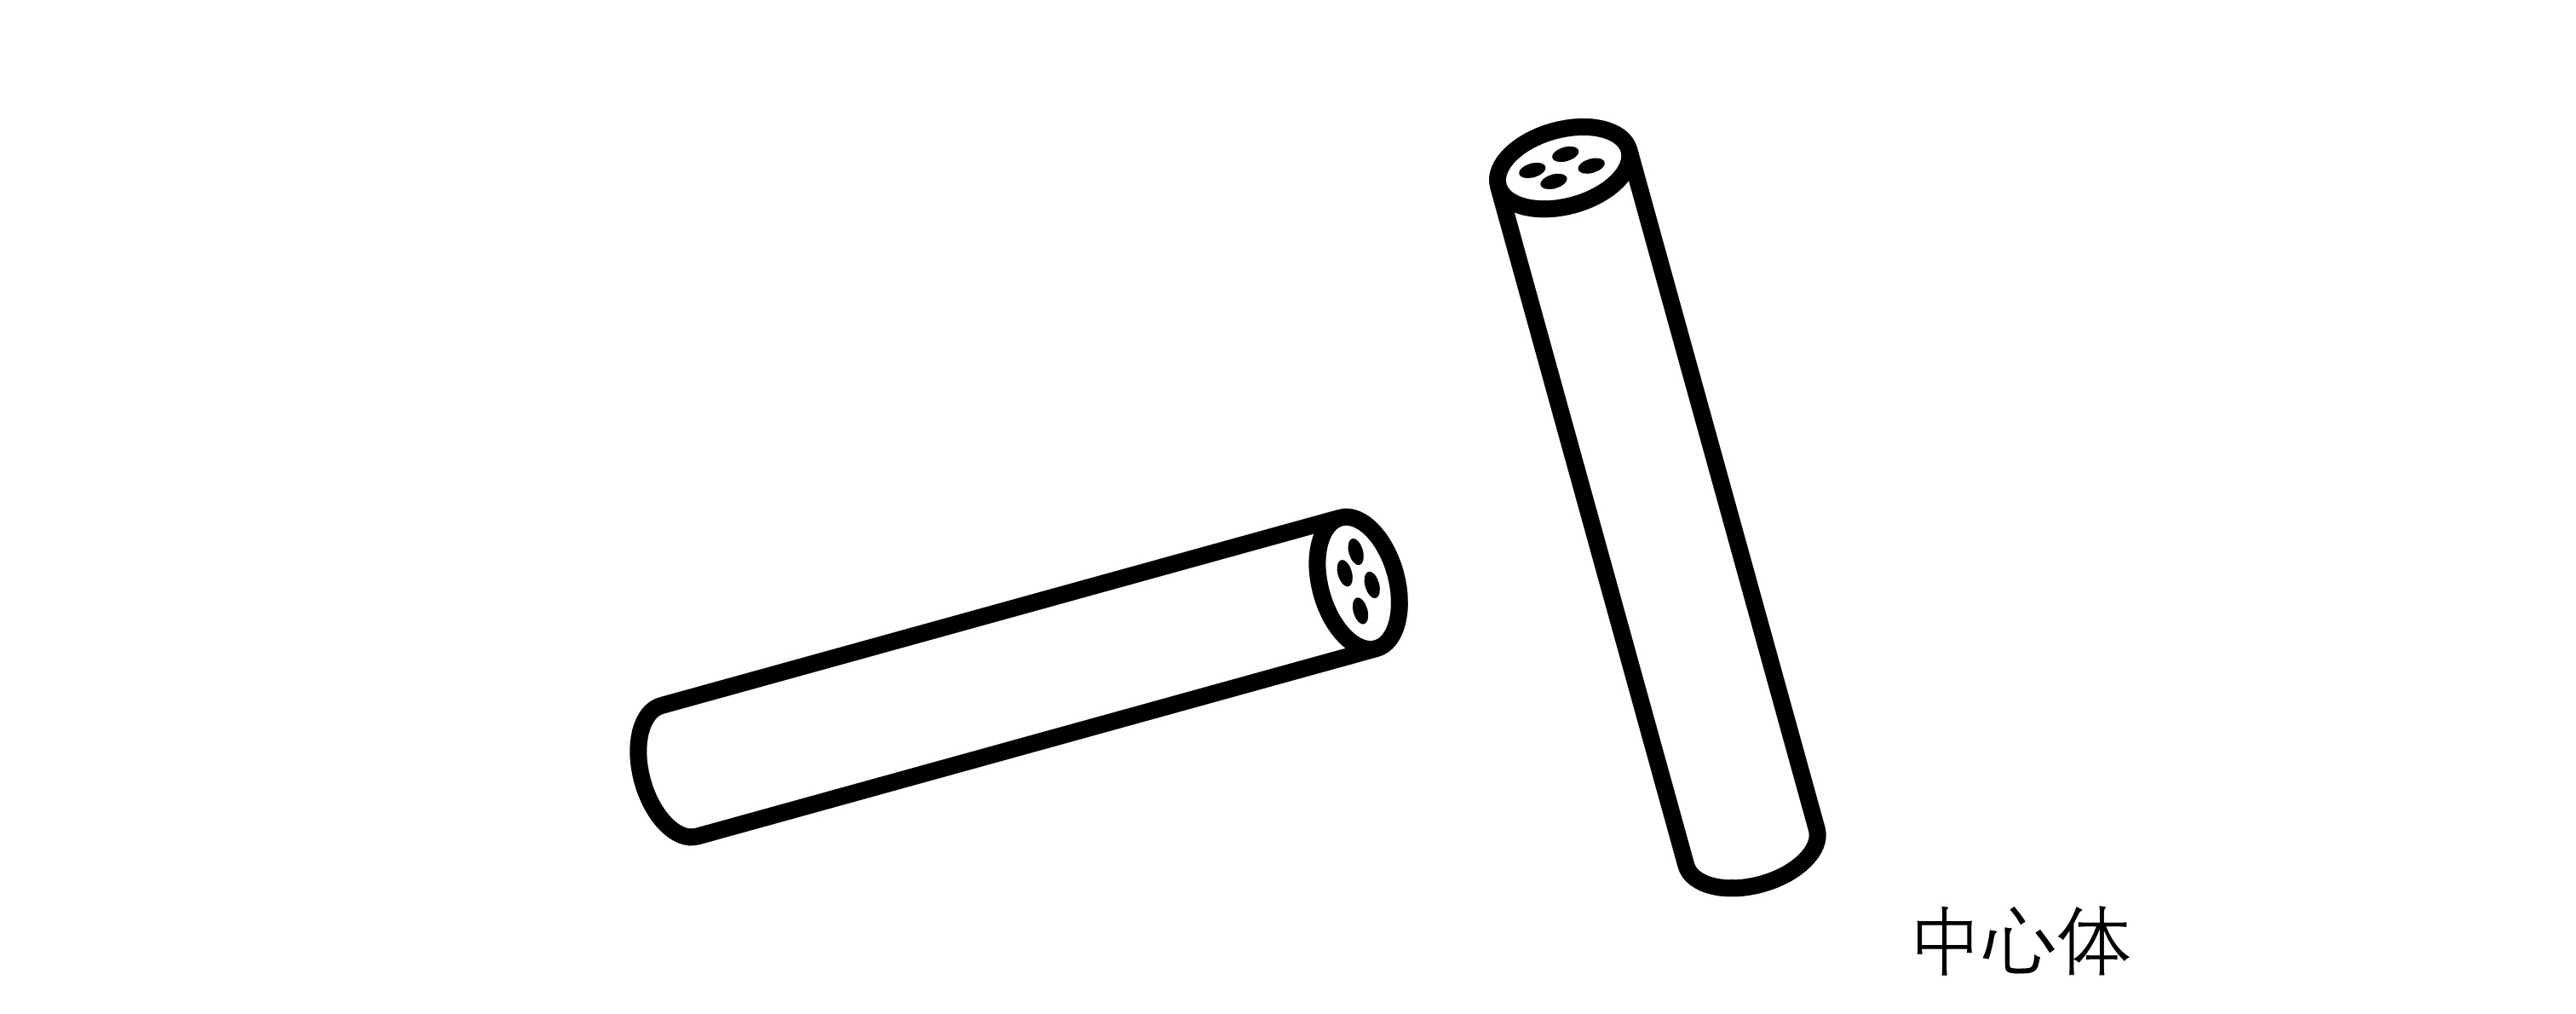
\includegraphics[width=9cm]{BiologyImage/9.jpg}
            \caption{中心体结构示意图}
        \end{center}
    \end{figure}\vspace{-32.5pt}

\subsubsection{溶酶体}
    溶酶体具有单层膜结构。\\[2mm]
    溶酶体是由膜围成的小球体,含有多种水解酶。\\[2mm]
    溶酶体可以分解衰老损坏的细胞器,溶酶体可以吞噬杀死入侵的病菌。
    \begin{figure}[h!]
        \begin{center}
            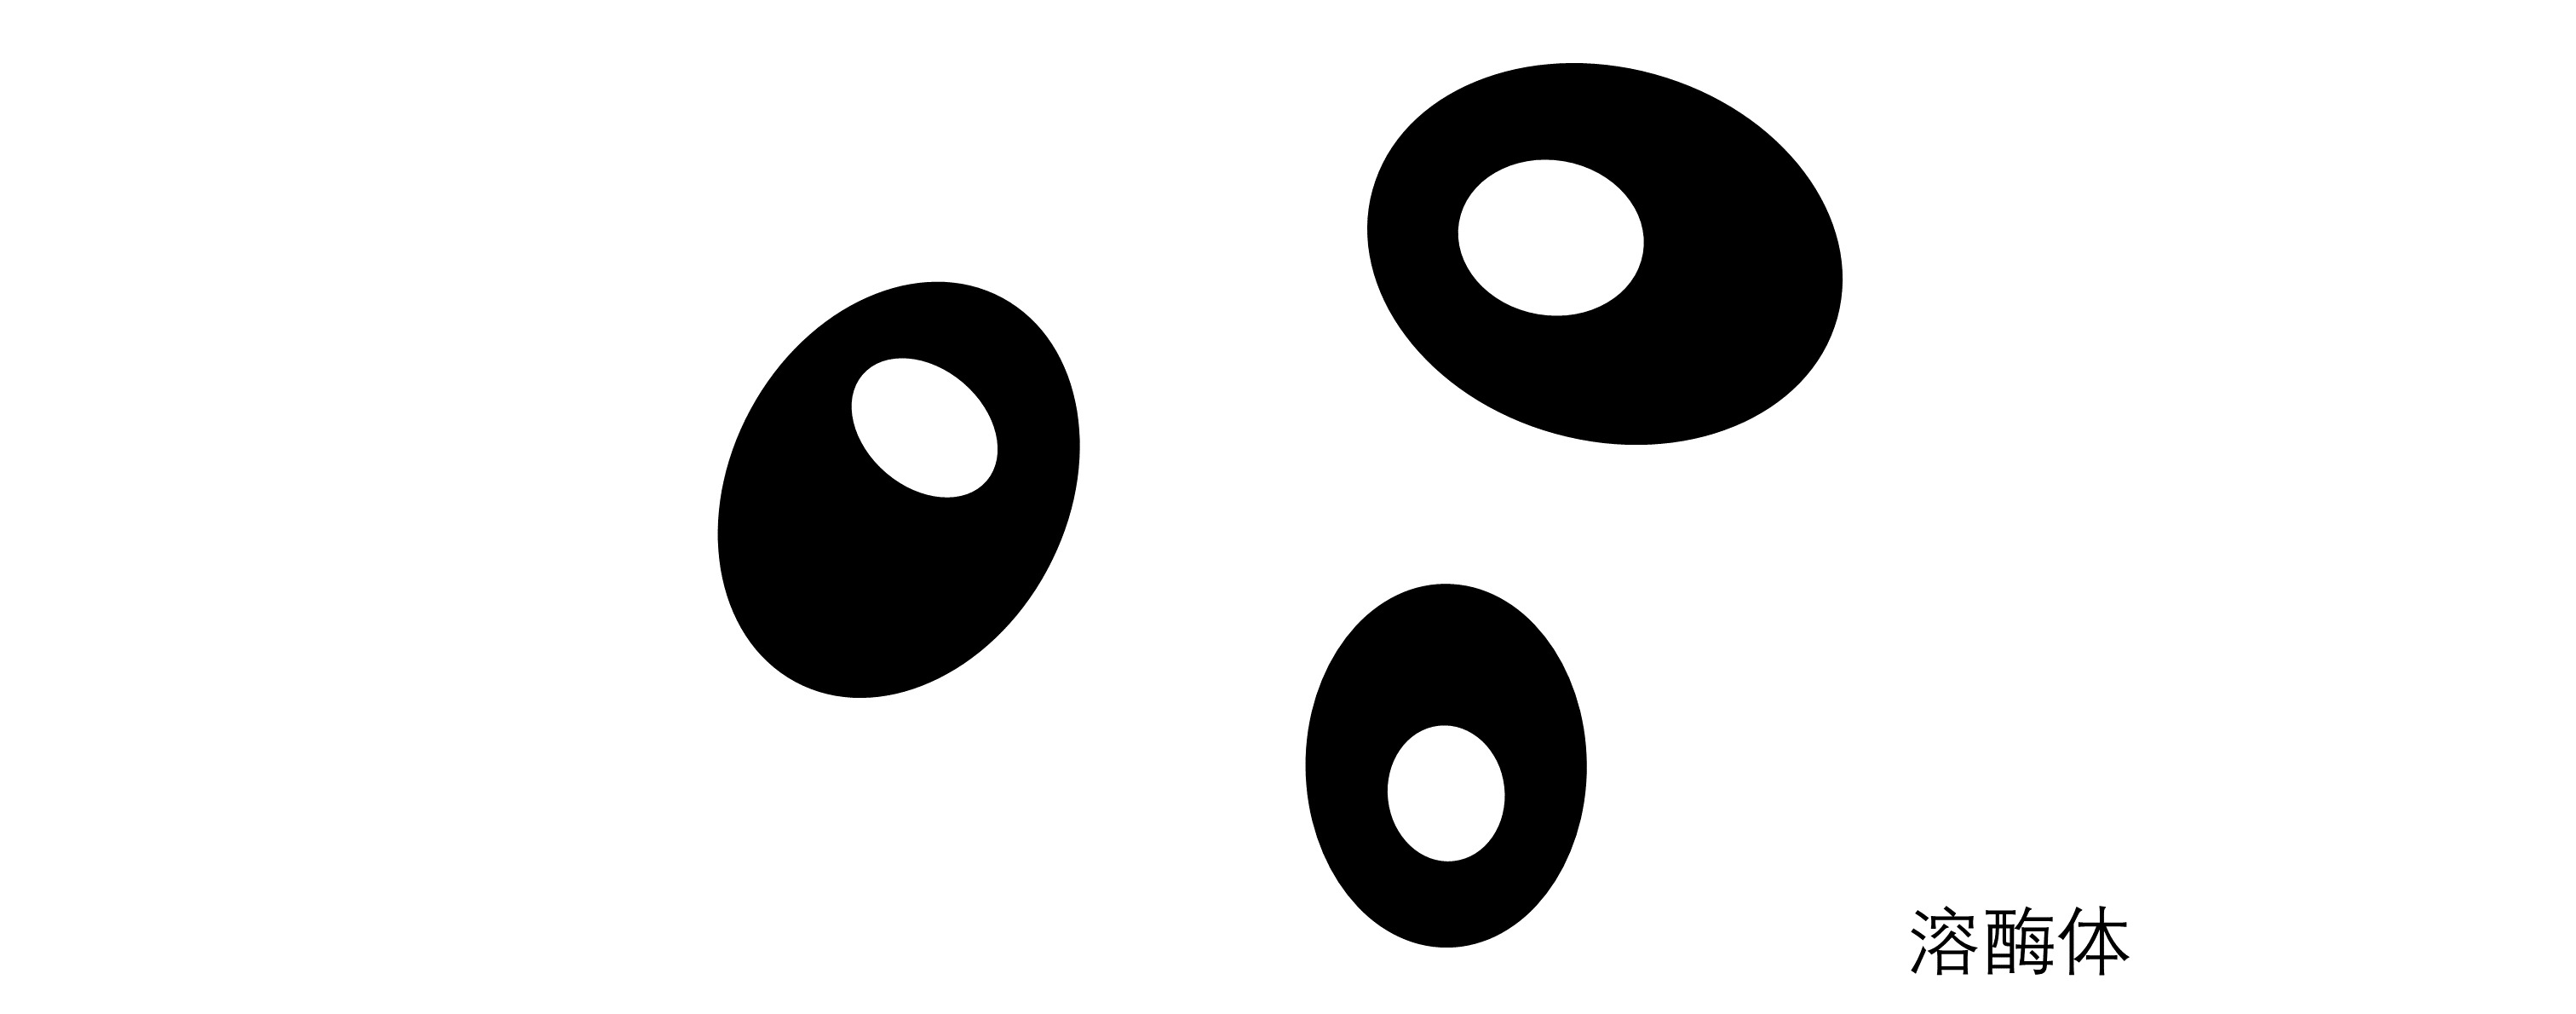
\includegraphics[width=9cm]{BiologyImage/10.jpg}
            \caption{溶酶体结构示意图}
        \end{center}
    \end{figure}

\newpage

\subsubsection{内质网}
    内质网具有单层膜结构。\\[3mm]
    内质网由彼此相同的网状膜系统组成,参与蛋白质的合成。\\[4mm]
    内质网可以具体分为粗面内质网和滑面内质网:\\[2mm]
    粗面内质网上有附着核糖体,参与蛋白质的加工运输。\\[2mm]
    滑面内质网上无附着核糖体,参与脂类的代谢。
    \begin{figure}[h]
        \begin{center}
            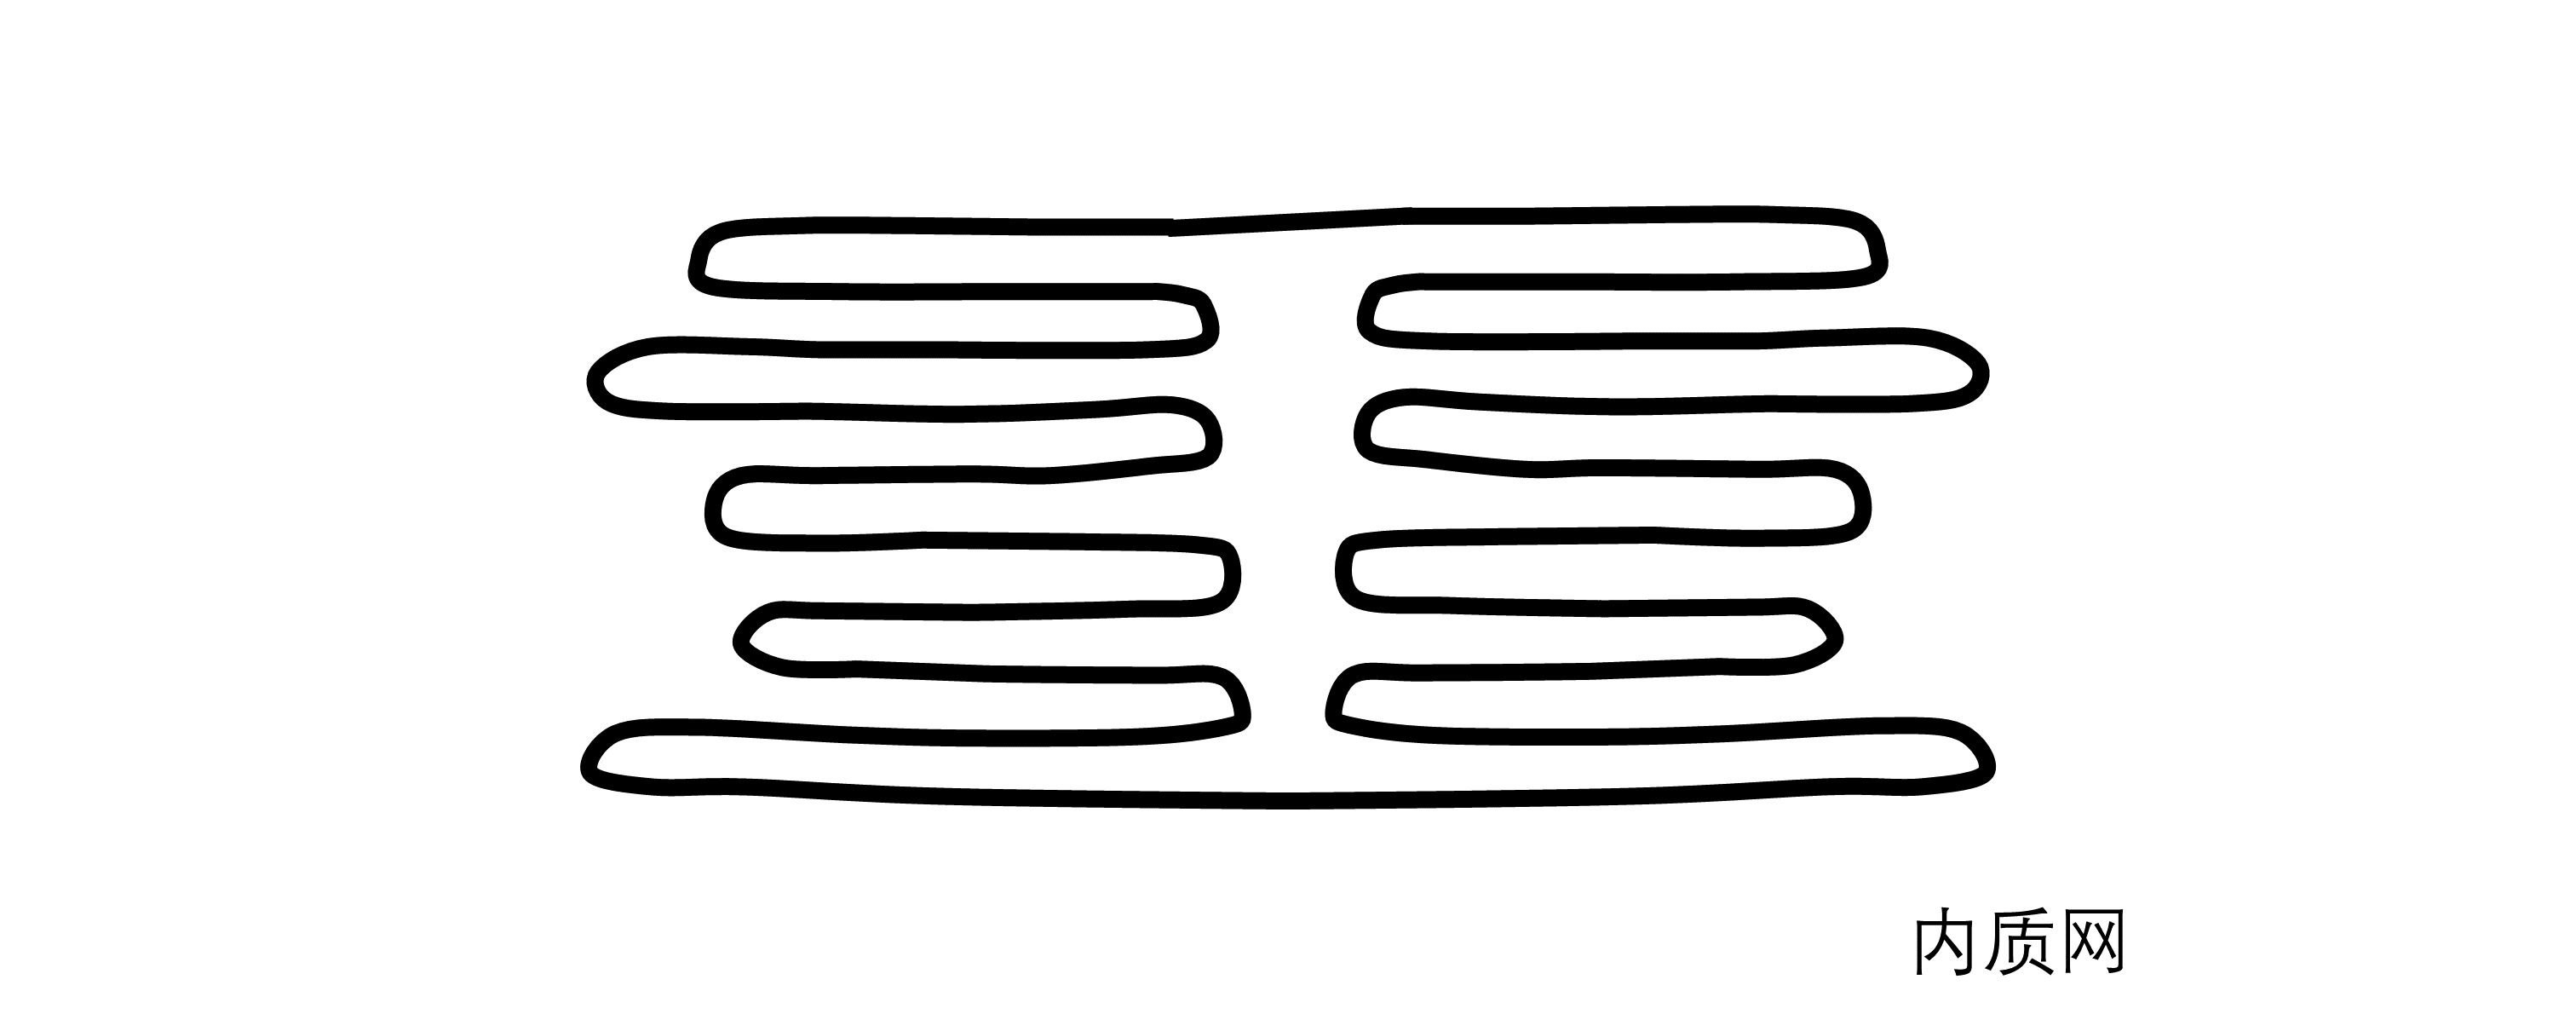
\includegraphics[width=9cm]{BiologyImage/6.jpg}
            \caption{内质网结构示意图}
        \end{center}
    \end{figure}

\subsubsection{高尔基体}
    高尔基体具有单层膜结构。\\[3mm]
    高尔基体由数层扁平囊和泡状结构组成,参与蛋白质的合成。\\[3mm]
    高尔基体起到物质的储存,加工,转运,分泌的作用。\\[3mm]
    高尔基体在植物中与合成细胞壁有关。\\[3mm]
    高尔基体在动物中与分泌蛋白质有关。
    \begin{figure}[h]
        \begin{center}
            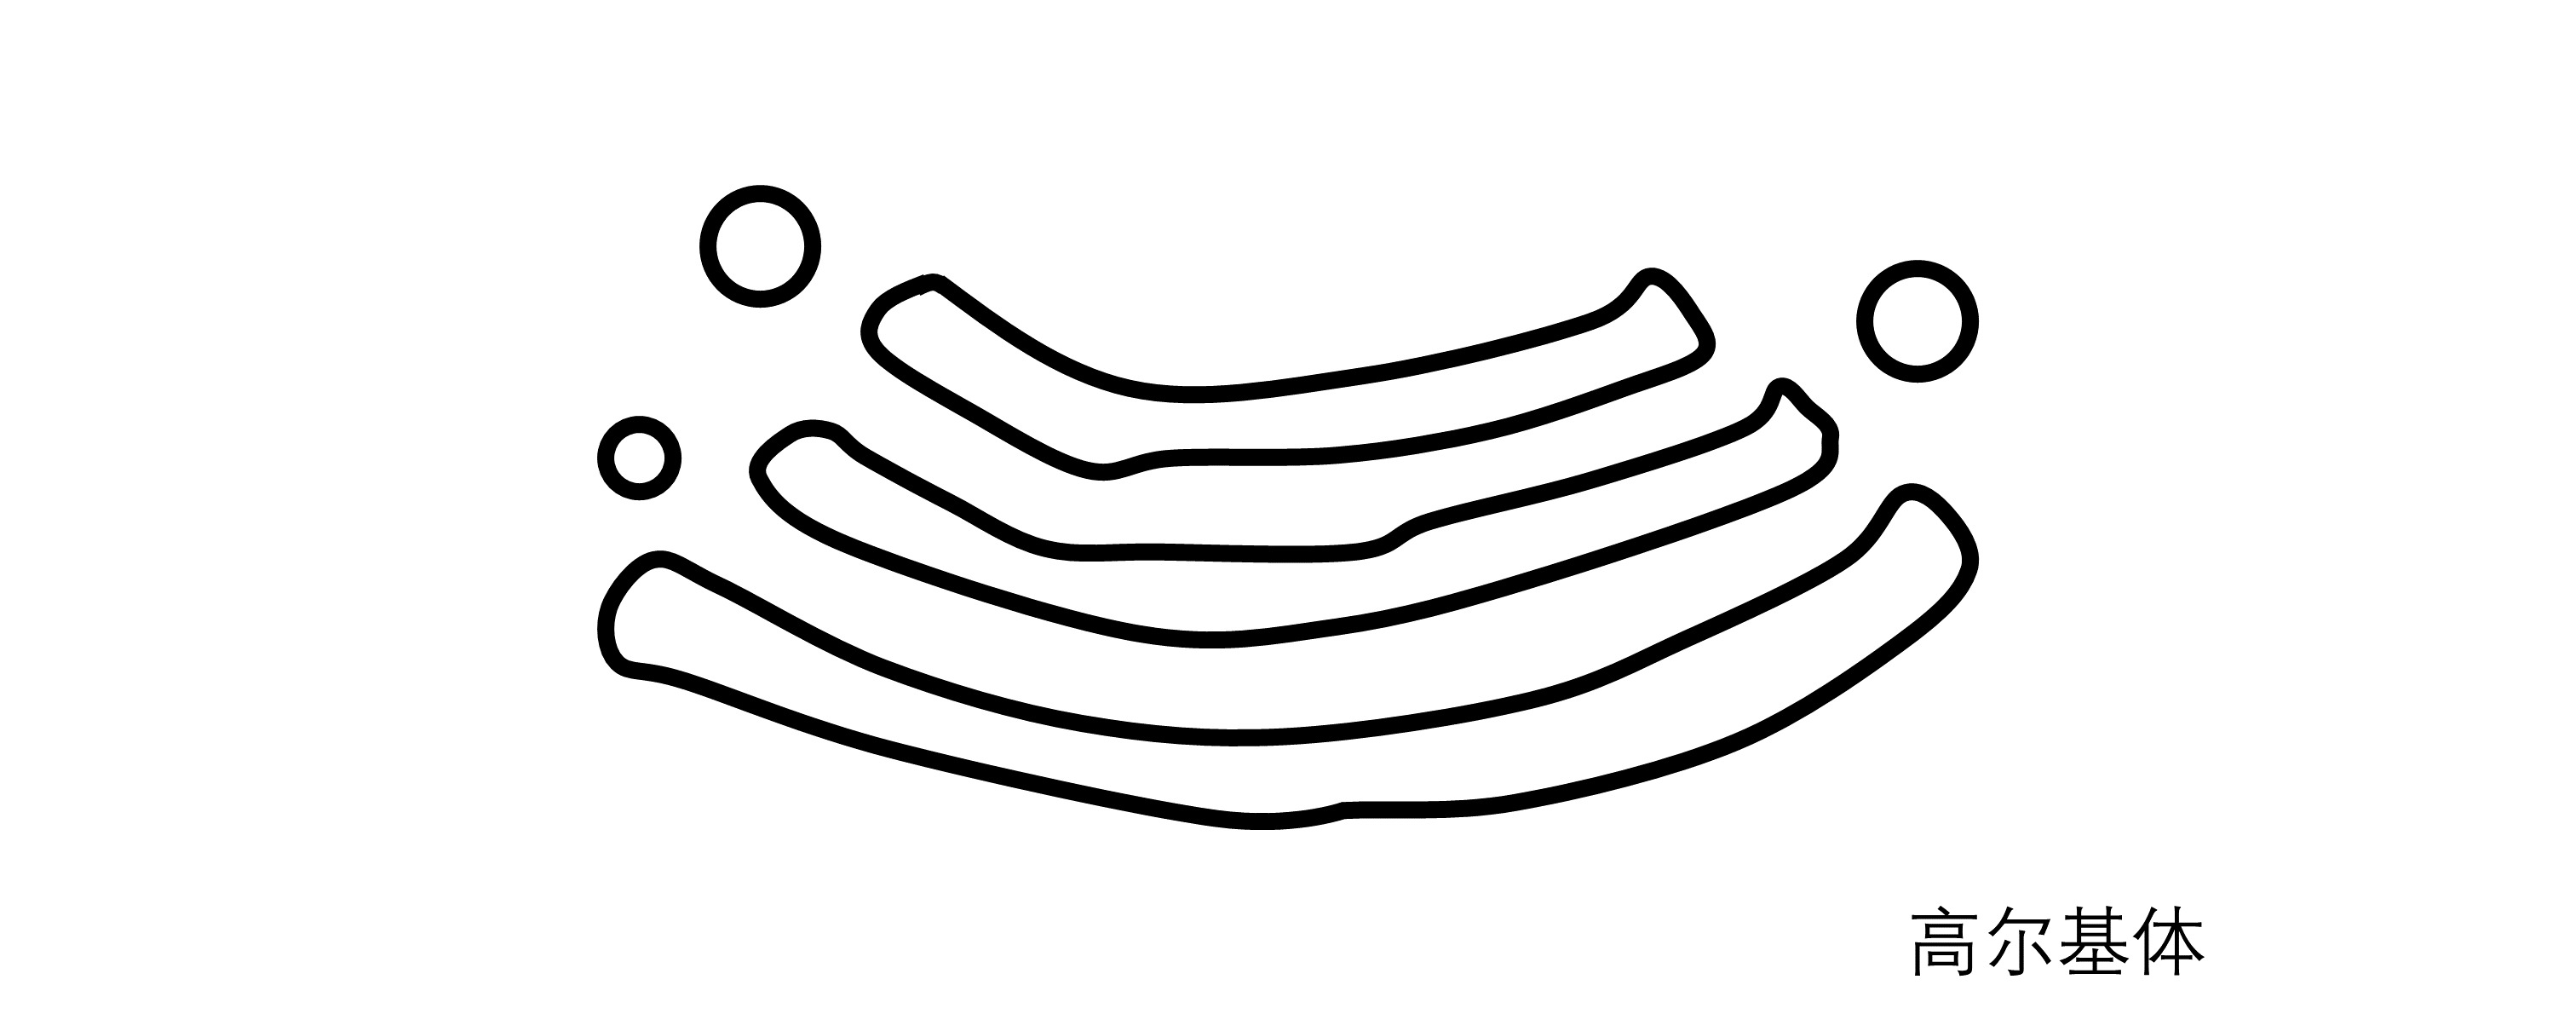
\includegraphics[width=9cm]{BiologyImage/5.jpg}
            \caption{高尔基体结构示意图}
        \end{center}
    \end{figure}
    
\newpage
    
\subsubsection{线粒体}
    线粒体具有双层膜结构。\\[3mm]
    线粒体由外膜和内膜组成,外膜光滑,内膜向内折叠成嵴。\\[3mm]
    线粒体是细胞进行呼吸作用的场所。
    \begin{figure}[h]
        \begin{center}
            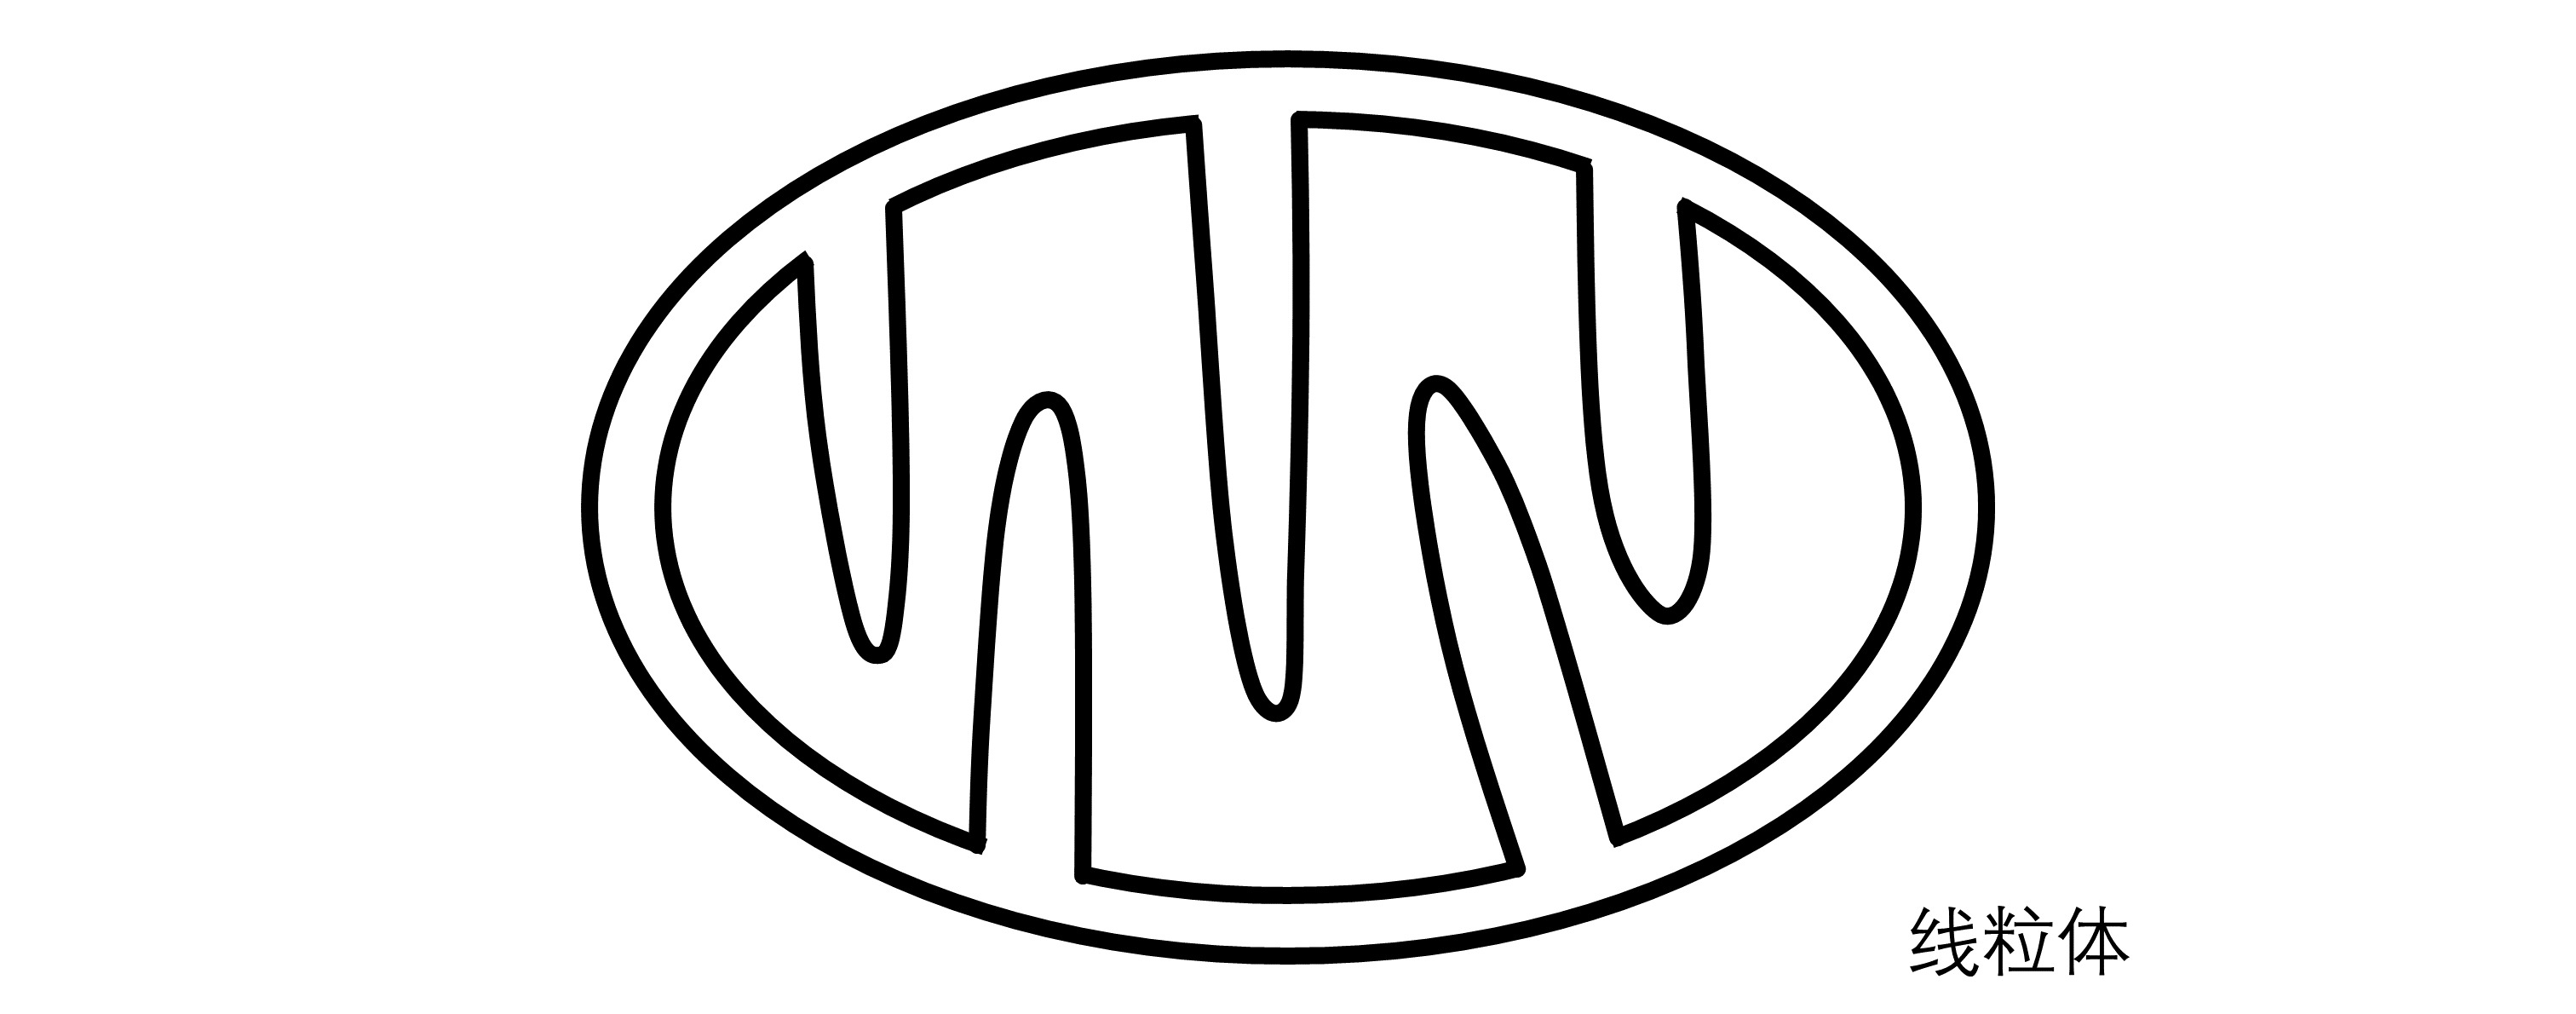
\includegraphics[width=9cm]{BiologyImage/7.jpg}
            \caption{线粒体结构示意图}
        \end{center}
    \end{figure}

\subsubsection{叶绿体}
    叶绿体具有双层膜结构。\\[3mm]
    叶绿体由外膜和内膜组成,内部包含由基粒构成的类囊体。\\[3mm]
    叶绿体是细胞进行光合作用的场所。
    \begin{figure}[h]
        \begin{center}
            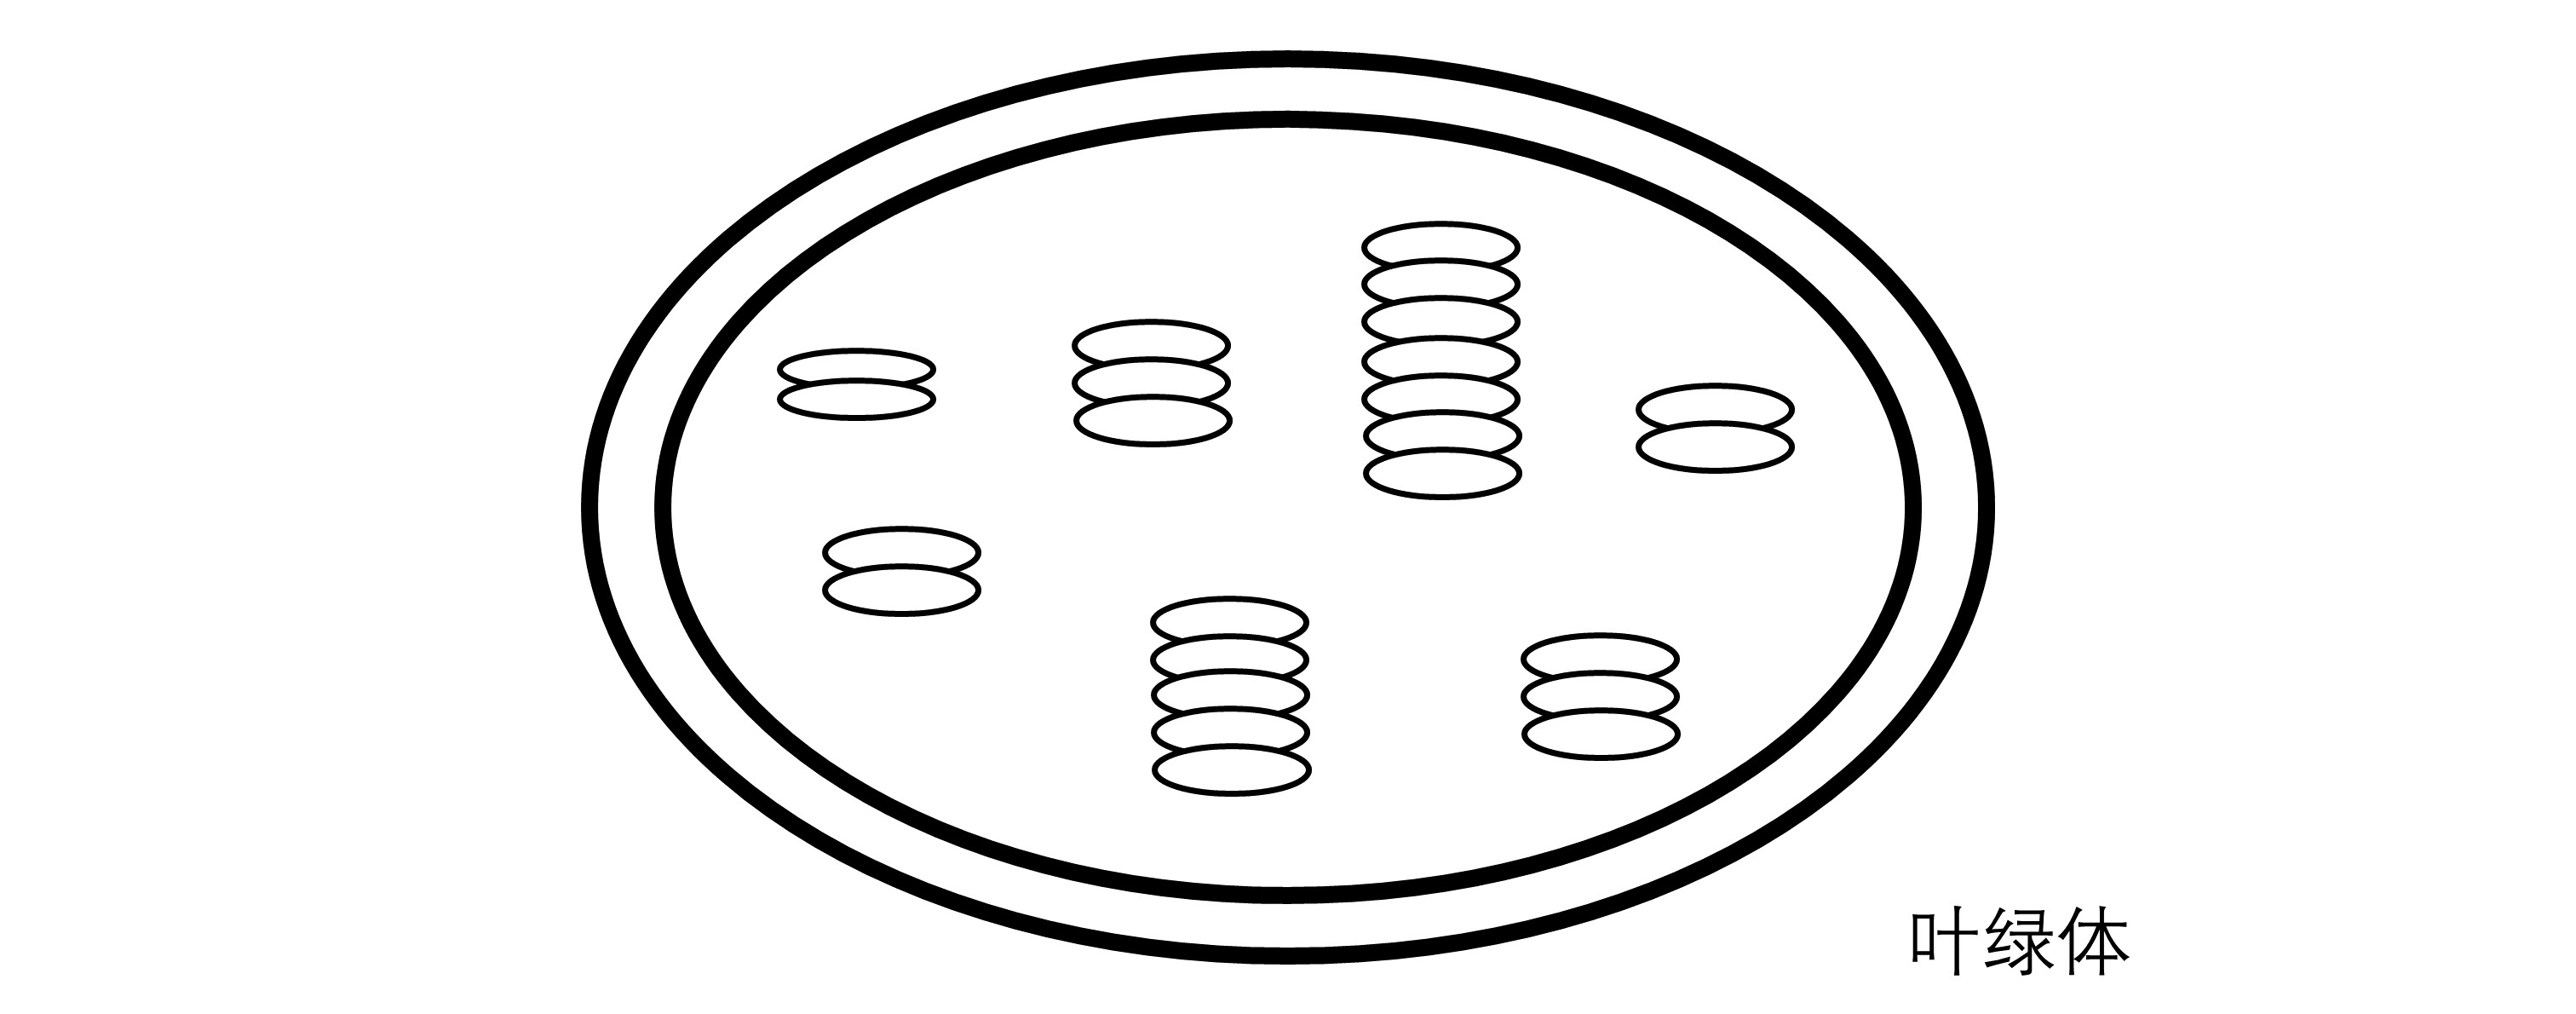
\includegraphics[width=9cm]{BiologyImage/8.jpg}
            \caption{叶绿体结构示意图}
        \end{center}
    \end{figure}

\newpage

\subsection{原核细胞与真核细胞}
    以下列出了原核细胞核真核细胞的差异:\vspace{5pt}
    \begin{table}[h]
        \begin{center}
            \begin{tabular}{l|l|l|l}
                \hline
                原核细胞\qquad&无成形细胞核\qquad&遗传物质储存在细胞中央\qquad&直径$1$-$10$微米\qquad\\ \hline
                真核细胞\qquad&有成形细胞核\qquad&遗传物质储存在细胞核中\qquad&直径$10$-$50$微米\qquad\\ \hline
            \end{tabular}
            \caption{原核细胞核真核细胞的差异}
        \end{center}
    \end{table}\\
    原核细胞仅有核糖体一种细胞器,原核细胞中储存遗传物质的位置称为拟核。\\[3mm]
    原核生物是由原核细胞构成的生物,颤藻是一种典型的原核生物。\\[3mm]
    真核生物是由真核细胞构成的生物,水棉是一种典型的真核生物。\\[6mm]
    细菌是一种广泛存在的原核生物,支原体,衣原体,立克次氏体也属于原核生物。\\[3mm]
    支原体的特点是没有细胞壁,衣原体的特点是需要寄生在活细胞中。\\

\subsection{非细胞结构的生物}
    病毒是一种非细胞结构的生物,体积通常在$150$纳米以下,需要通过电子显微镜观察。\\[3mm]
    病毒由核酸和蛋白质构成,核酸位于病毒中心,蛋白质位于病毒外侧,构成衣壳。\\[3mm]
    病毒的遗传物质核酸可以是DNA或RNA,但是对于同一种病毒只能具有一种类型的核酸。\\[3mm]
    病毒需要寄生于活细胞才能存活,寄生状态时可以快速复制增殖,非寄生状态时呈结晶状态。\\[6mm]
    依据病毒的遗传物质类型,可以将其分为:DNA病毒,RNA病毒。\\[3mm]
    依据病毒的宿主细胞类型,可以将器分为:动物病毒,植物病毒,细菌病毒。\\[3mm]
    腺病毒是典型的DNA病毒,烟花草叶病毒是典型的RNA病毒。\\[3mm]
    细菌病毒也称为噬菌体,侵染细菌后会导致细菌裂解死亡,噬菌体也属于DNA病毒。

\newpage

\section{生命体内的化学反应}
    将外界物质转变为自身物质的过程称为同化作用。\\[3mm]
    将自身物质转变为外界物质的过程称为异化作用。\\[3mm]
    同化作用和异化作用组成了生物体的新陈代谢,新陈代谢需要依靠一系列化学反应完成。

\subsection{合成反应}
    合成反应是由小分子形成大分子的化学反应,每两个分子间的连接会产生一份水。\\[3mm]
    典型的合成反应:单糖合成为多糖,脂肪酸和甘油合成为脂肪,核苷酸合成为核酸。

\subsection{水解反应}
    水解反应是由大分子形成小分子的化学反应,每两个分子间的断裂会消耗一份水。\\[3mm]
    典型的分解反应:多糖分解为单糖,脂肪分解为脂肪酸和甘油,核酸分解为核苷酸。

\subsection{氧化分解反应}
    氧化分解反应是指在分解过程中释放能量的化学反应。\\[3mm]
    典型的氧化分解反应:葡萄糖被氧化分解为丙酮酸,脂肪酸被氧化分解为二碳化合物。

\subsection{酶}
    酶是一种由活细胞产生的生物大分子,
    酶在生物体内可以起到催化反应的作用。\\[3mm]
    酶的化学本质:大部分的酶是蛋白质,少部分酶是核糖核酸。\\[3mm]
    酶的高效性:通常情况下,酶的催化效率远远高于无机催化剂。\\[3mm]
    酶的专一性:特定的酶只能对特定的反应起到催化作用,
    这是因为酶分子中存在一个特定的活性部位,
    只有当活性部位与底物在结构上完全契合时才能起到催化作用。\\[3mm]
    酶具有一定的活性范围,每一种酶只有处在其特定的温度区间和酸度区间内时才能表现出活性,
    如果环境条件无法满足要求,酶的活性就会下降甚至彻底失活。\\[3mm]
    酶有时需要与一些辅助因子结合后才能显示活性,这些辅助因子通常是金属离子或有机小分子,
    这些辅助因子也通常称为辅酶,与氧化还原反应有关的酶通常都需要与辅酶结合才能显示活性。\\[3mm]
    酶活性的抑制有两种方式:竞争性抑制,非竞争性抑制。\\[3mm]
    竞争性抑制:产生与底物结构类似的物质占据酶的活性部位,使得底物无法与酶反应。\\[3mm]
    非竞争性抑制:产生可以与酶结合使得活性部位结构发生改变的物质,使得底物无法与酶反应。

\newpage
    
\subsection{腺苷三磷酸}
    生命的活动需要能量,糖类等有机物质中虽然可以储存能量,但是释放能量却需要一定的时间,
    这是因为糖类所储存的是“稳定的化学能”,而生命活动需要的是“活跃的化学能”。\\[3mm]
    科学研究表明,为生命活动直接供能的是一种被称为腺苷三磷酸的物质。\\[3mm]
    腺苷三磷酸中包含了以下结构:一个腺嘌呤,一个核糖,三个磷酸基团。\\[3mm]
    腺苷三磷酸中相邻的磷酸基团间的化学键非常活跃,称为高能磷酸键,断裂时释放大量能量。\\[6mm]
    下图展示了腺苷三磷酸吸收能量和释放能量的过程:\vspace{5pt}
    \begin{figure}[h!]
        \begin{center}
            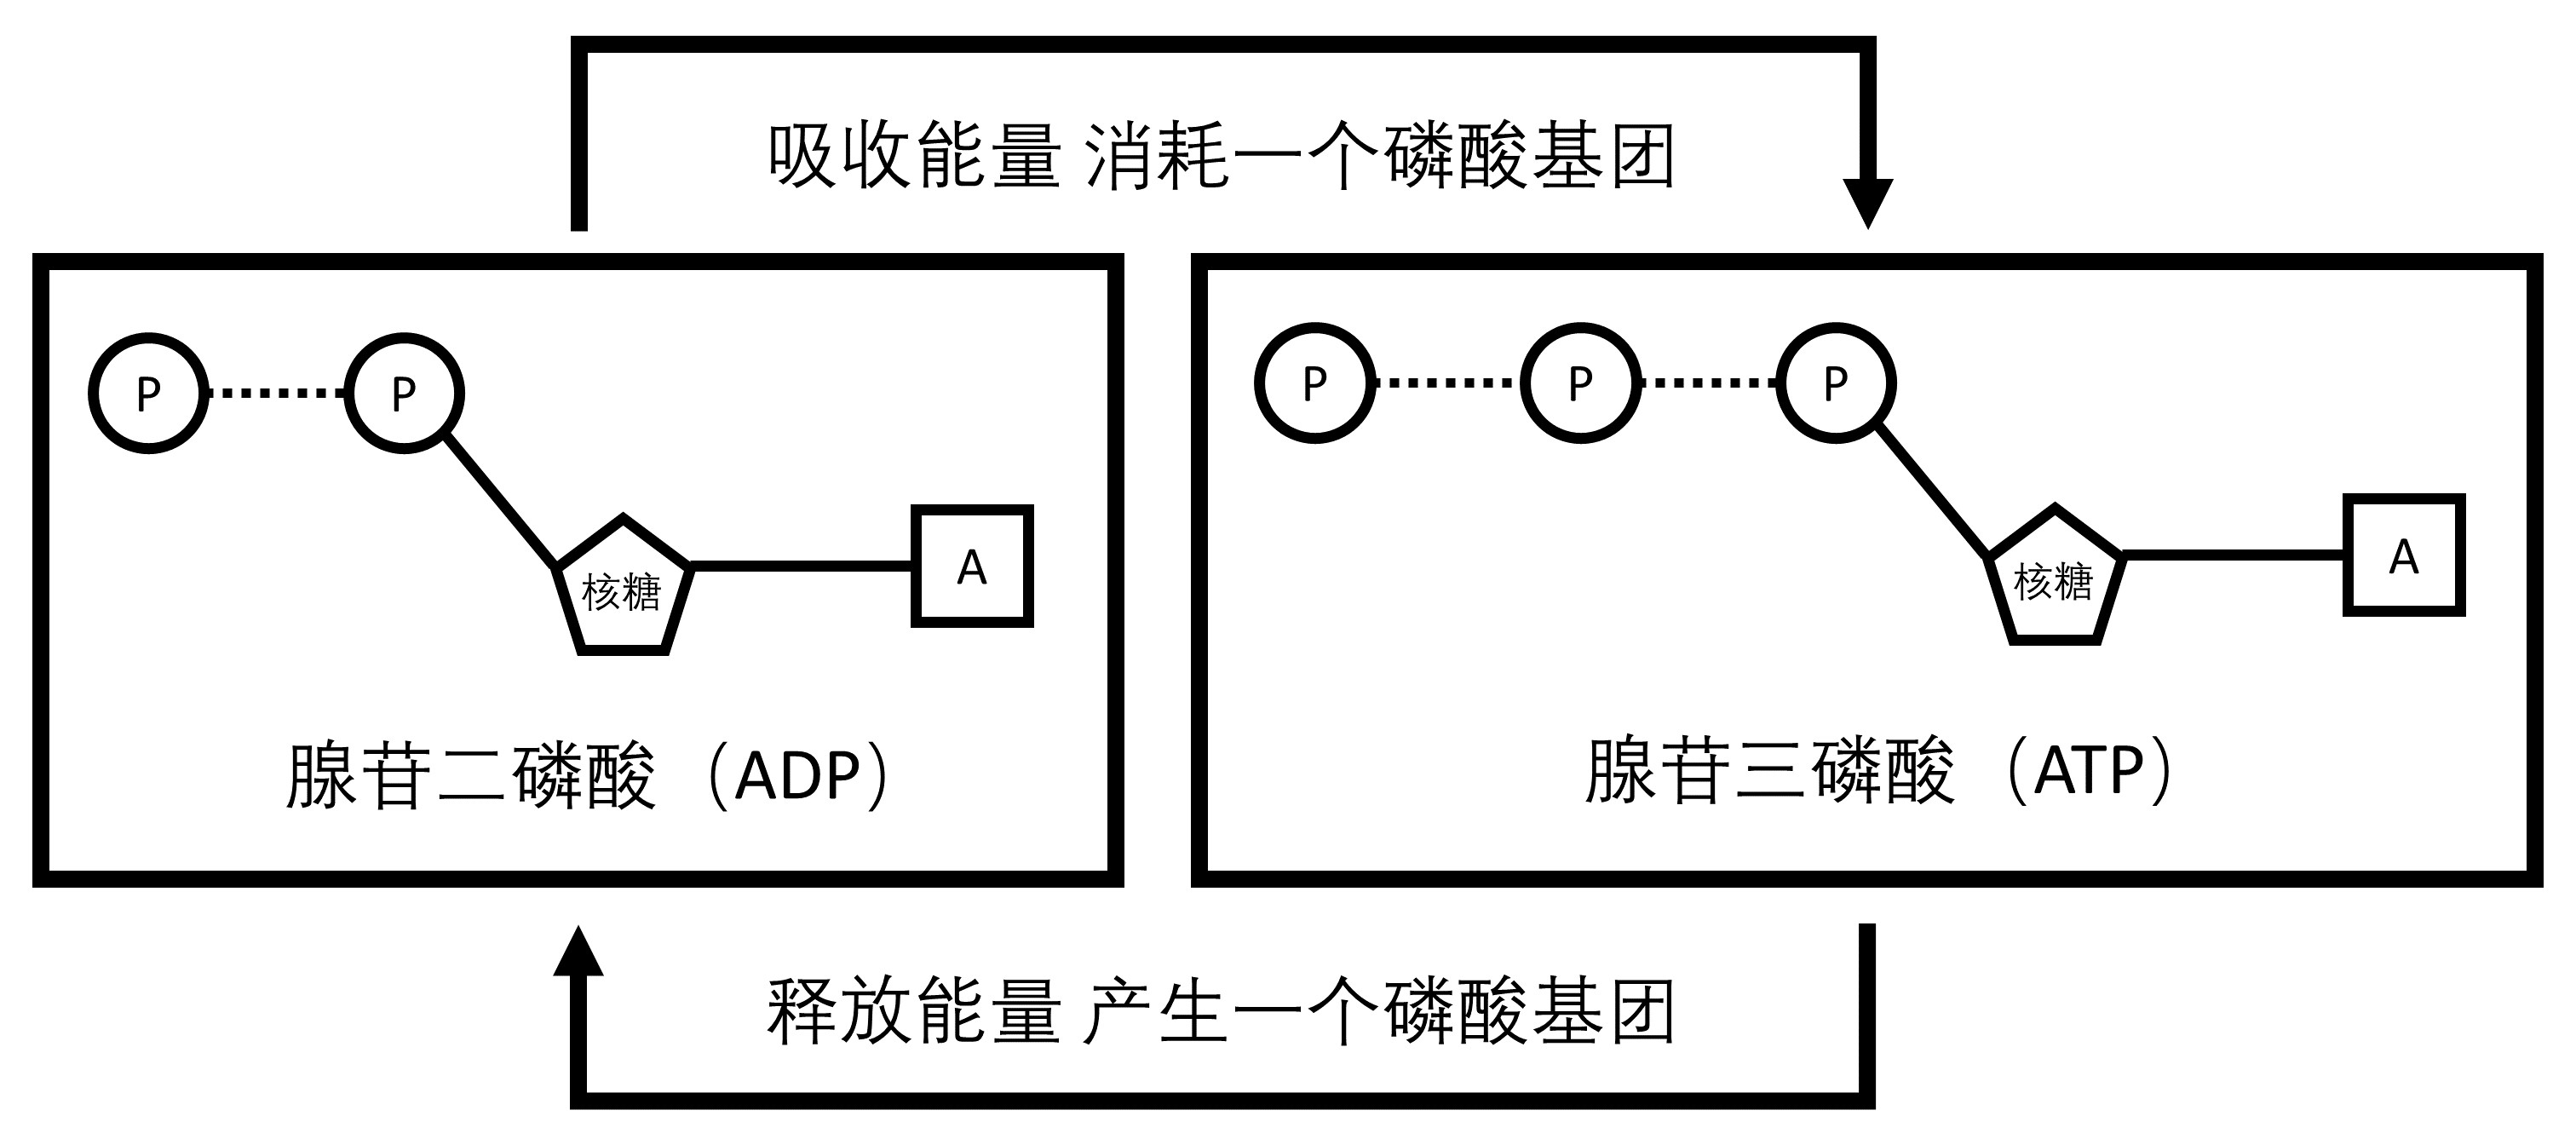
\includegraphics[width=10cm]{BiologyImage/11.jpg}
            \caption{腺苷三磷酸的能量吸收和释放}
        \end{center}
    \end{figure}\\
    当细胞消耗能量时,腺苷三磷酸的高能磷酸键断裂,变为腺苷二磷酸,释放能量。\\[3mm]
    当细胞产生能量时,腺苷二磷酸的高能磷酸键产生,变为腺苷三磷酸,吸收能量。\\[3mm]
    由于存在这样一个循环,腺苷三磷酸成为了生命活动的直接能源,形象的被称为能量货币。\\[3mm]
    在某些特殊情况下,腺苷二磷酸的高能磷酸键也会断裂,产物称为腺苷一磷酸。\\[6mm]
    腺苷三磷酸的简称为ATP,其中T代表磷酸基团的数量为3个。\\[3mm]
    腺苷二磷酸的简称为ADP,其中D代表磷酸基团的数量为2个。\\[3mm]
    腺苷一磷酸的简称为AMP,其中M代表磷酸基团的数量为1个。\\[3mm]
    磷酸基团的简称为Pi,其中i是为了与磷元素区分而添加。
    
\newpage
    
\subsection{光合作用}
    光合作用:在光照条件下,叶绿体吸收二氧化碳和水,释放出氧气,产生有机物质。\\[3mm]
    光合作用的反应方程式:
    \begin{center}
        \ce{CO2 + H2O ->T[光能][叶绿体] (CH2O) + O2 ^}\\[4mm]
    \end{center}
    光合作用的示意图:
    \begin{figure}[h!]
        \begin{center}
            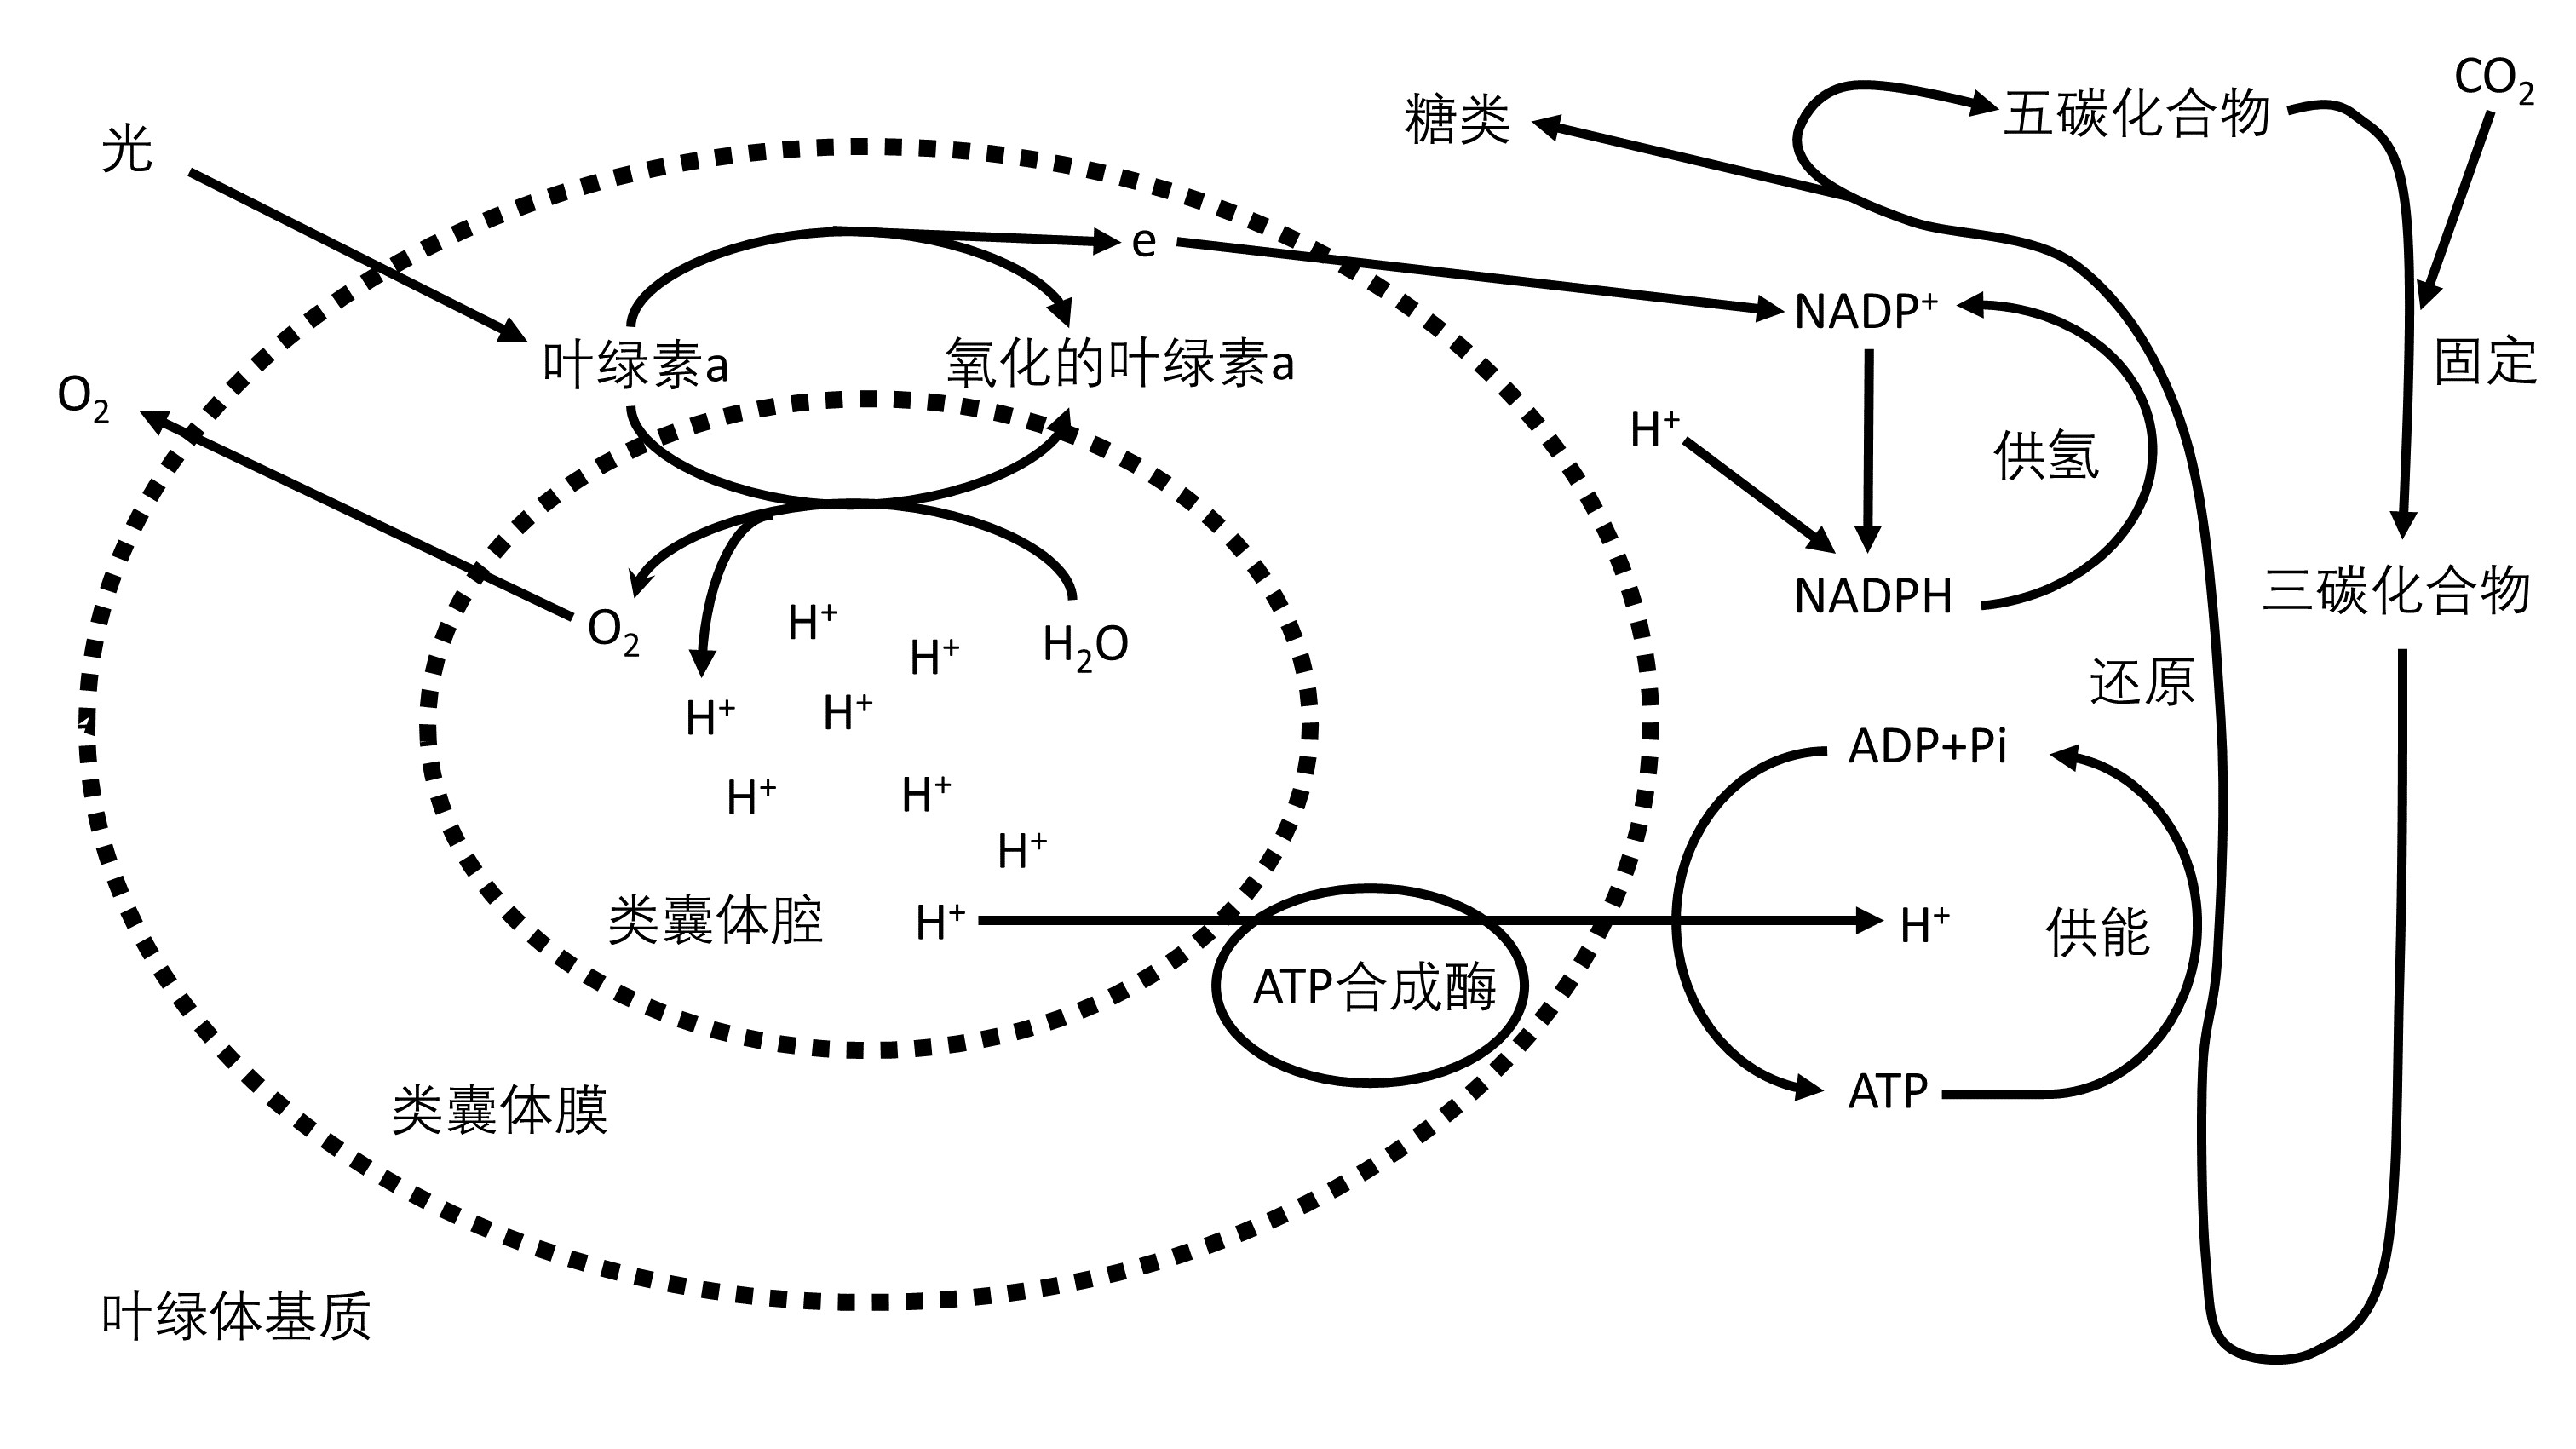
\includegraphics[width=11cm]{BiologyImage/12.jpg}
            \caption{光合作用}
        \end{center}
    \end{figure}\vspace{-20pt}
    
\subsubsection{光反应}
    光反应中,光能变为了活跃的化学能。\\[3mm]
    1.类囊体膜上的叶绿素a吸收了阳光的能量,
    释放出了一个电子e,并变为了氧化的叶绿素a。\\[3mm]
    2.第一步中氧化的的叶绿素a具有强氧化性,从类囊体腔中的水中夺取电子,
    迫使水发生光解,产生氧气和氢离子,氧气释放,氢离子积蓄在类囊体腔中。
    当积累到一定浓度时,氢离子经过类囊体膜上的ATP合成酶到达叶绿体基质,
    过程中释放出能量,使得ADP和Pi合成ATP。\\[3mm]
    3.第一步中释放出的电子e在类囊体膜上经过一系列传递,最终传递至叶绿体基质中的\ce{NADP+},
    使得第二步中叶绿体基质中的~\ce{H+}与~\ce{NADP+}结合形成~\ce{NADPH}。
    
\subsubsection{暗反应}
    暗反应中,活跃的化学能变为了稳定的化学能。\\[3mm]
    1.固定:在叶绿体基质中,一份二氧化碳和一份五碳化合物反应,产生两份三碳化合物。\\[3mm]
    2.还原:在叶绿体基质中,第一步的三碳化合物通过光反应的产物,ATP供能,NADPH供氢,一部分重新变为五碳化合物,一部分变为糖类物质。
    
\newpage

\subsubsection{叶绿体中的色素}
    以下表格列举了叶绿体中四种色素的特点:\vspace{8pt}
    \begin{table}[h]
        \begin{center}
            \begin{tabular}{l|l|l|l}
                \hline
                色素名称\qquad\qquad&色素颜色\qquad\qquad&吸收光谱\qquad\qquad\qquad&层析顺序\qquad\qquad\\ \hline
                叶绿素a&蓝绿色&红橙光和蓝紫光&2\\ \hline
                叶绿素b&黄绿色&红橙光和蓝紫光&1\\ \hline
                叶黄素&黄色&蓝紫光&3\\ \hline
                胡萝卜素&橙黄色&蓝紫光&4\\ \hline
            \end{tabular}
            \caption{叶绿体中色素的特点}
        \end{center}
    \end{table}\\
    需要说明的是,表中的层析顺序是自下向上排列的。\\[3mm]
    叶绿素a和叶绿素b可以统称为叶绿素,叶黄素和胡萝卜素可以统称为类胡萝卜素。\\

\subsubsection{光合作用的强度}
    光合作用的强度也称为光合速率。\\[3mm]
    光合速率可以使用单位时间内释放的\ce{O2}表示。\\[3mm]
    光合速率可以使用单位时间内消耗的\ce{CO2}表示。\\[6mm]
    光照强度可以影响光合速率,随着光照强度的增强,光合速率逐渐增加并趋向于定值。\\[3mm]
    光照强度为条件时,光合速率趋向的定值被称为光饱和点。\\[3mm]
    光照强度是夜晚对光合速率的主要限制因素。\\[6mm]
    二氧化碳浓度可以影响光合速率,随着二氧化碳浓度的增加,光合速率逐渐增加并趋向于定值。\\[3mm]
    二氧化碳浓度为条件时,光合速率趋向的定值被称为二氧化碳饱和点。\\[3mm]
    二氧化碳浓度是白天对光合速率的主要限制因素。\\[6mm]
    温度对光合速率影响较大,随者温度增加,光合速率表现为先增加后减小。\\[3mm]
    高温和低温会导致气孔关闭,导致暗反应的原料二氧化碳减少,同时暗反应的酶活性也会下降。

\newpage
    
\subsection{呼吸作用}
    呼吸作用可以分为两类:有氧呼吸和无氧呼吸。\\[3mm]
    呼吸作用的示意图:
    \begin{figure}[h!]
        \begin{center}
            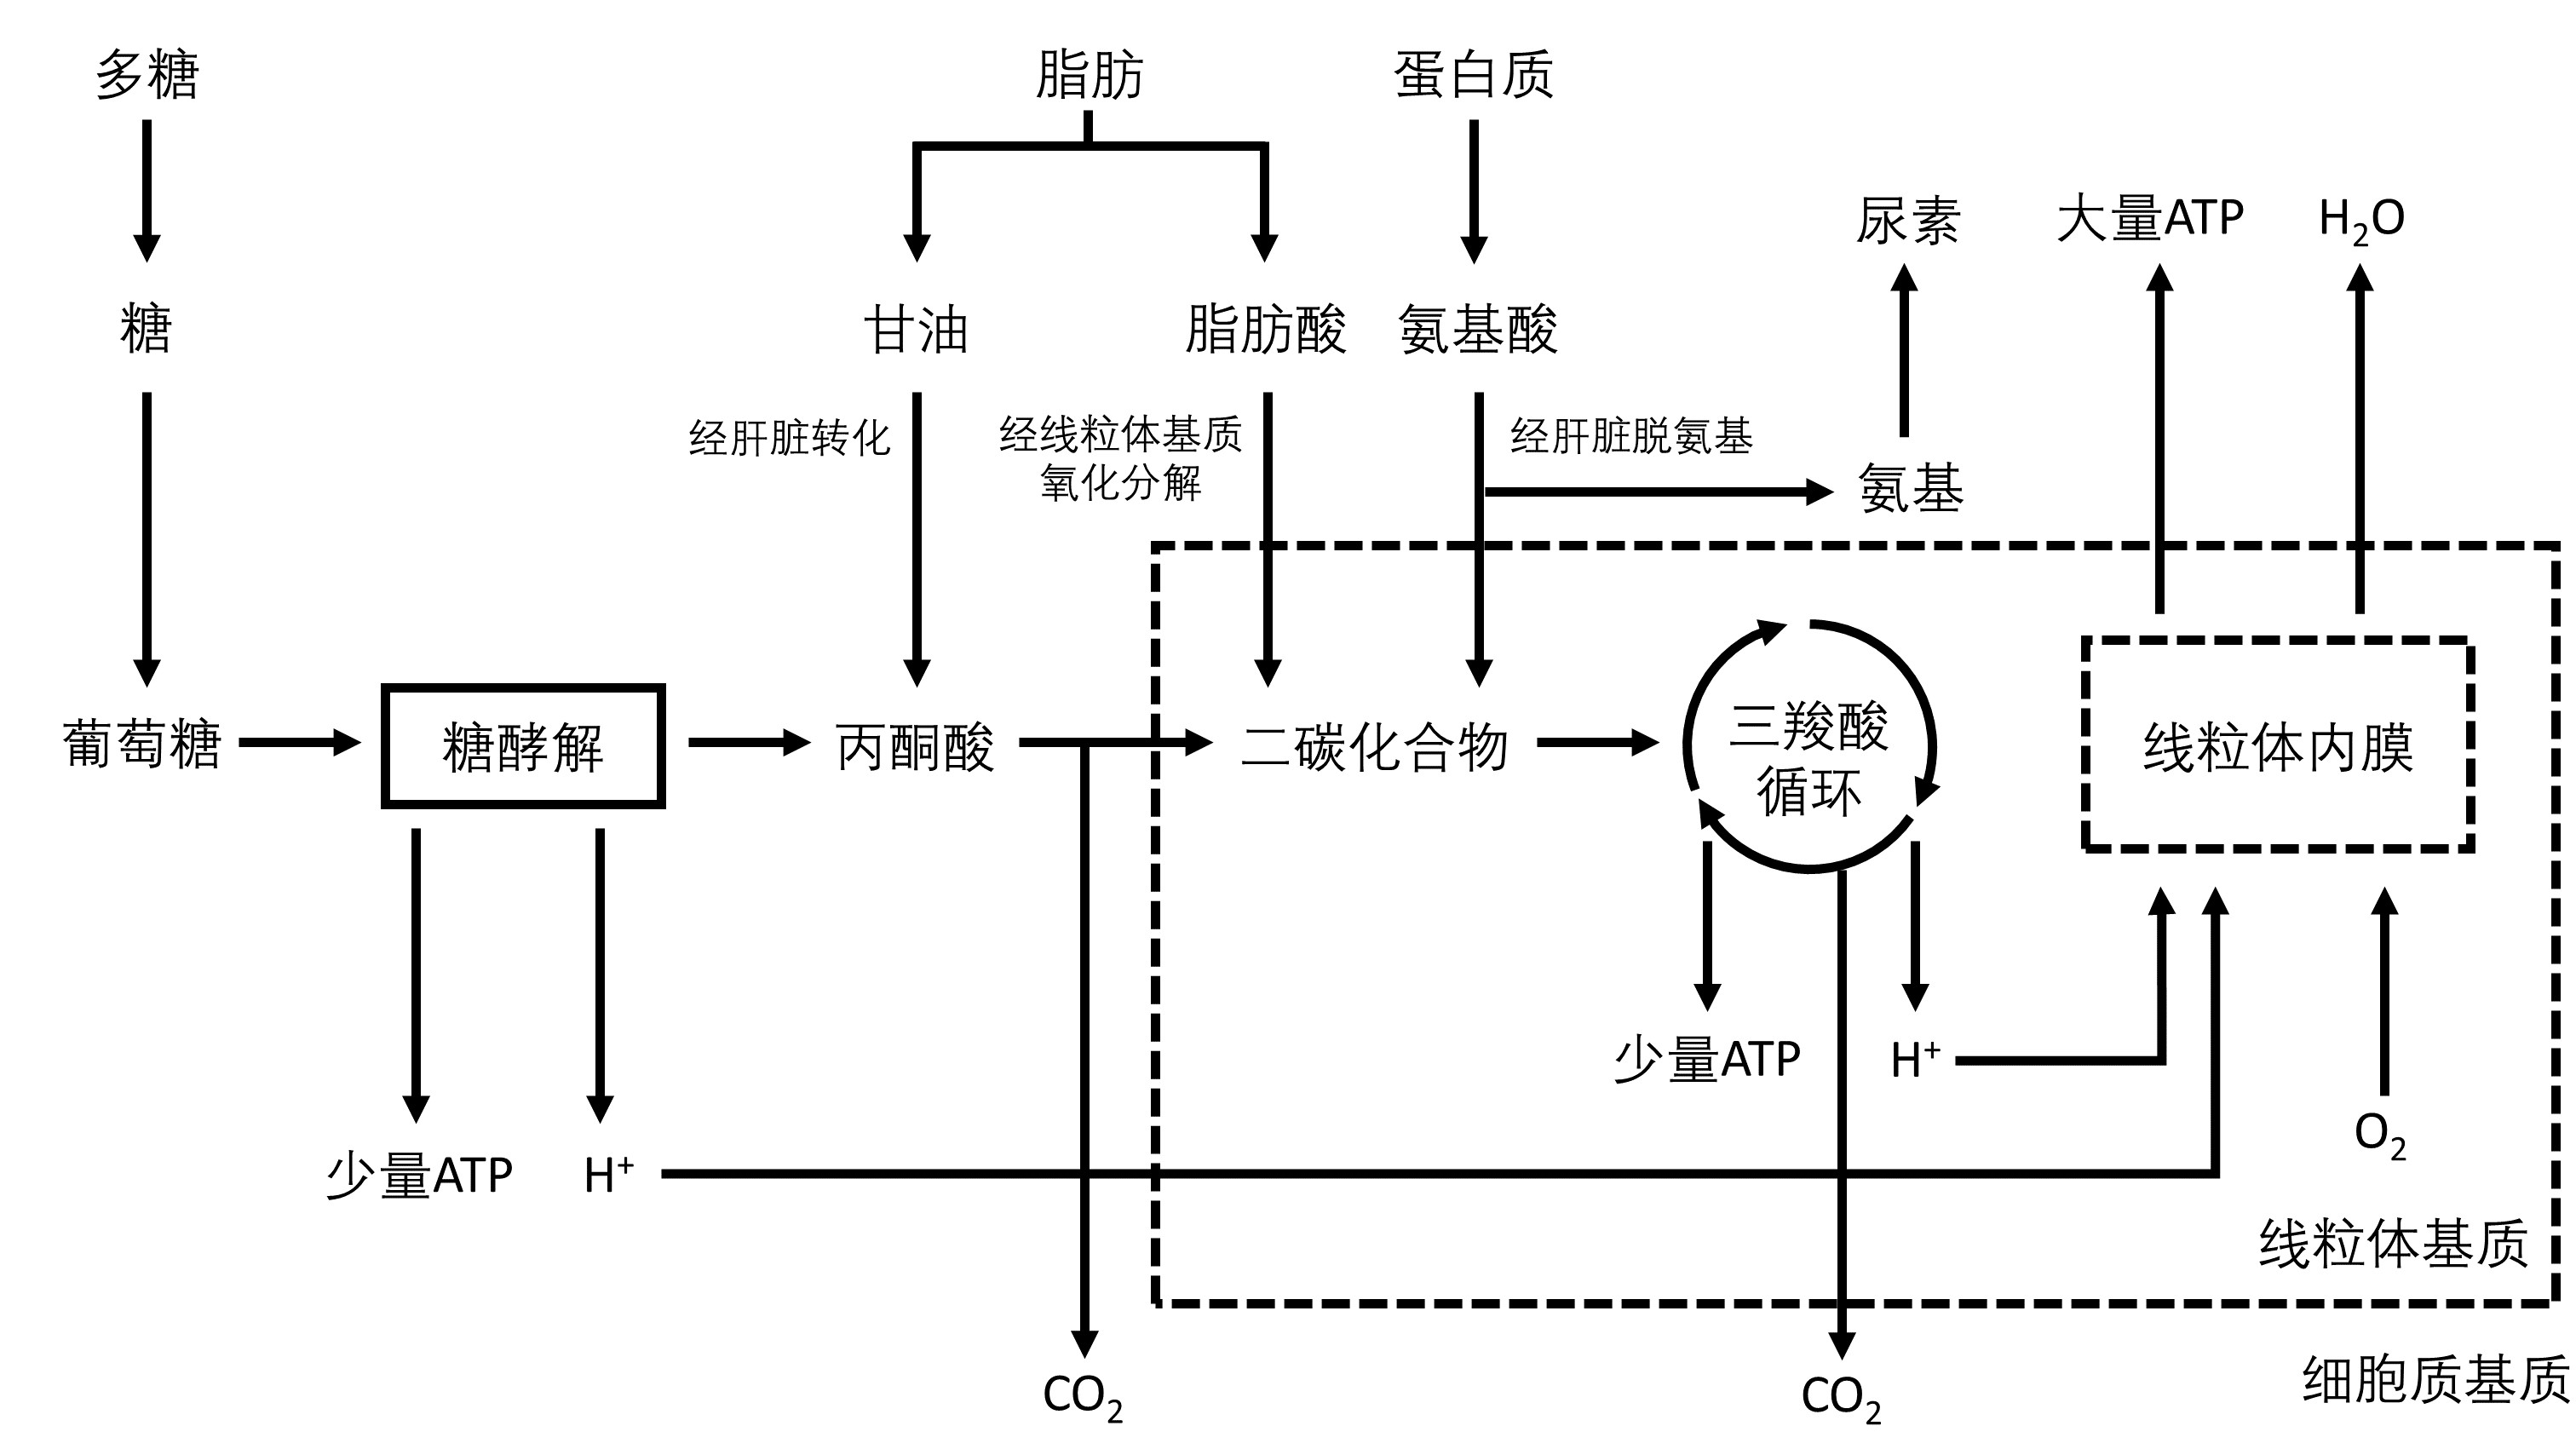
\includegraphics[width=11cm]{BiologyImage/13.jpg}
            \caption{呼吸作用}
        \end{center}
    \end{figure}\vspace{-30pt}
    
\subsubsection{有氧呼吸}
    有氧呼吸:在有氧气的条件下,有机物氧化分解生成大量二氧化碳和水,产生大量能量。\\[3mm]
    有氧呼吸的反应方程式:
    \begin{center}
        \ce{C6H12O6 + 6O2 -> 6CO2 + 6H2O}\\[4mm]
    \end{center}
    1.葡萄糖在细胞质基质中氧化分解,转化为丙酮酸,产生~\ce{H+},产生少量ATP。\\[3mm]
    2.丙酮酸在线粒体基质中氧化分解,转化为二碳化合物,产生\ce{CO2}。\\[3mm]
    3.二碳化合物加入三羧酸循环彻底氧化分解,产生~\ce{H+},产生\ce{CO2},产生少量ATP。\\[3mm]
    4.生成的~\ce{H+}在辅酶的携带下到达线粒体内膜与\ce{O2}反应,产生\ce{H2O},产生大量ATP。\\[3mm]
    第一步中葡萄糖氧化分解为丙酮酸的过程也称为糖酵解。\\[5mm]
    以下是其他营养物质在呼吸作用中的代谢途径:\vspace{5pt}
    \begin{table}[h]
        \begin{center}
            \begin{tabular}{l|l}
                \hline
                多糖-单糖\qquad\qquad&加入葡萄糖的代谢途径\qquad\qquad\\ \hline
                脂肪-甘油\qquad\qquad&加入丙酮酸的代谢途径\qquad\qquad\\ \hline
                脂肪-脂肪酸\qquad\qquad&加入二碳化合物的代谢途径\qquad\qquad\\ \hline
                蛋白质-氨基酸\qquad\qquad&加入二碳化合物的代谢途径\qquad\qquad\\ \hline
            \end{tabular}
            \caption{营养物质的代谢途径}
        \end{center}
    \end{table}

\newpage

\subsubsection{无氧呼吸}
    无氧呼吸:在五氧气的条件下,有机物氧化分解生成酒精或乳酸,产生少量能量。\\[3mm]
    无氧呼吸的反应反应方程式:
    \begin{center}
        \begin{tabular}{rl}
            &\ce{C6H12O6 -> 2C2H6O + 2CO2}\\[3mm]
            &\ce{C6H12O6 -> 2C3H6O3}\\[5mm]
        \end{tabular}
    \end{center}
    无氧呼吸中,糖酵解的产物丙酮酸不会进入线粒体,而是停留在细胞质基质中。\\[3mm]
    对于产物是酒精的无氧呼吸,丙酮酸随后会接受来自辅酶的~\ce{H+},同时脱去~\ce{CO2},生成酒精。\\[3mm]
    对于产物是乳酸的无氧呼吸,丙酮酸随后会接受来自辅酶的~\ce{H+},生成乳酸。\\[6mm]
    通常将微生物在无氧条件下的呼吸称为发酵。\\[3mm]
    酵母菌无氧呼吸的产物是酒精,也称为酒精发酵。\\[3mm]
    乳酸菌无氧呼吸的产物是酒精,也称为乳酸发酵。\\[6mm]
    动物无氧呼吸时的产物是乳酸,植物无氧呼吸的产物是酒精,但马铃薯无氧呼吸的产物是乳酸。\\[3mm]
    人在剧烈运动时,由于短时间内供氧不足,导致肌细胞内缺少氧气,使得肌细胞进行无氧呼吸,
    这个过程中乳酸大量堆积在肌细胞,因此造成了肌肉酸痛的感觉。

\newpage

\section{生物体对信息的传递和调节}

\subsection{感受器}
    单细胞生物通过整个细胞感受外界刺激,而高等动物则通过自身特定的感受器感受特定的刺激,
    这些刺激通过神经系统传递至大脑,在大脑皮层产生感觉。

\subsubsection{皮肤感受器}
    通过皮肤,我们可以感受到物体的温度,形状,这是因为我们皮肤中存在大量传感器。\\[3mm]
    皮肤感受器在人的手指和嘴唇等部分分布较多,所以这些部位也较为敏感。\\[3mm]
    皮肤中存在以下四种感受器:痛感受器,冷传感器,温感受器,接触感受器,压力感受器。

\subsubsection{光感受器}
    以人为首的高等生物的光感受器通常是眼。\\[3mm]
    眼睛中可以感受光照的细胞称为视细胞,视细胞又可以分为视锥细胞和视杆细胞。\\[3mm]
    视锥细胞:可以感受光照,可以感受色彩,对光的敏感度弱,只能在强光下工作。\\[3mm]
    视杆细胞:可以感受光照,不能感受色彩,对光的敏感度强,可以在弱光下工作。\\[3mm]
    视锥细胞和视杆细胞的互补使得我们,白天可以看到物体的色彩,晚上可以看清物体的轮廓。

\subsubsection{声波感受器}
    以人为首的高等生物的声波感受器通常是耳。\\[3mm]
    耳朵可以分为三部分:外耳,中耳,内耳。\\[3mm]
    外耳可以收集声波,使其沿外耳道向内传播至鼓膜,引起鼓膜振动。\\[3mm]
    中耳可以将鼓膜的振动,传递到三块彼此以关节相连的听小骨。\\[3mm]
    内耳中的耳蜗可以将由听小骨传递的声波转换为神经冲动,传递至大脑皮层形成听觉。\\[3mm]
    内耳中还有一个称为前庭器的器官,由前庭和三个半规管组成,是感受身体平衡的器官。

\subsubsection{化学感受器}
    人和脊椎动物的化学感受器主要分布于鼻腔的嗅粘膜和口腔的舌上。\\[3mm]
    嗅细胞:嗅粘膜上分布有嗅细胞,可以感受溶于嗅粘膜表面具有气味的化学物质。\\[3mm]
    味细胞:舌上分布有味蕾,味细胞分布于味蕾顶端的小孔中,感受溶于水中的化学分子。

\newpage

\subsubsection{动物感受器}
    鱼类的侧线属于物理感受器,可以感受水流和方位。\\[3mm]
    蛇类的颊窝属于物理感受器,可以感受红外线。\\[3mm]
    昆虫的嗅毛属于化学感受器,可以感受气味。

\subsection{神经系统}
    组成神经系统的基本单位是神经细胞,也被称为神经元,神经元由细胞体,轴突,树突组成。\\[3mm]
    细胞体:神经元的营养和代谢中心,内含细胞核和细胞器。\\[3mm]
    树突:树突较短,具有较多的分支,是神经元传入信息的部位。\\[3mm]
    轴突:轴突较长,具有较少的分支,是神经元传出信息的部分。\\[3mm]
    髓鞘:套在轴突上的结构,对轴突起到绝缘作用。\\[3mm]
    神经纤维是对树突轴突以及髓鞘三者的合称。

\subsubsection{神经冲动传导}
    在神经细胞质膜的内外两侧存在电位差,称为膜电位。\\[3mm]
    静息电位:膜外电位为正,膜内电位为负,外正内负。\\[3mm]
    动作电位:膜外电位为负,膜内电位为正,外负内正。\\[3mm]
    膜电位中,正电位由~\ce{Na+}离子维持,负电位由~\ce{K+}离子维持。\\[3mm]
    神经冲动传导示意图:\vspace{-5pt}
    \begin{figure}[h]
        \begin{center}
            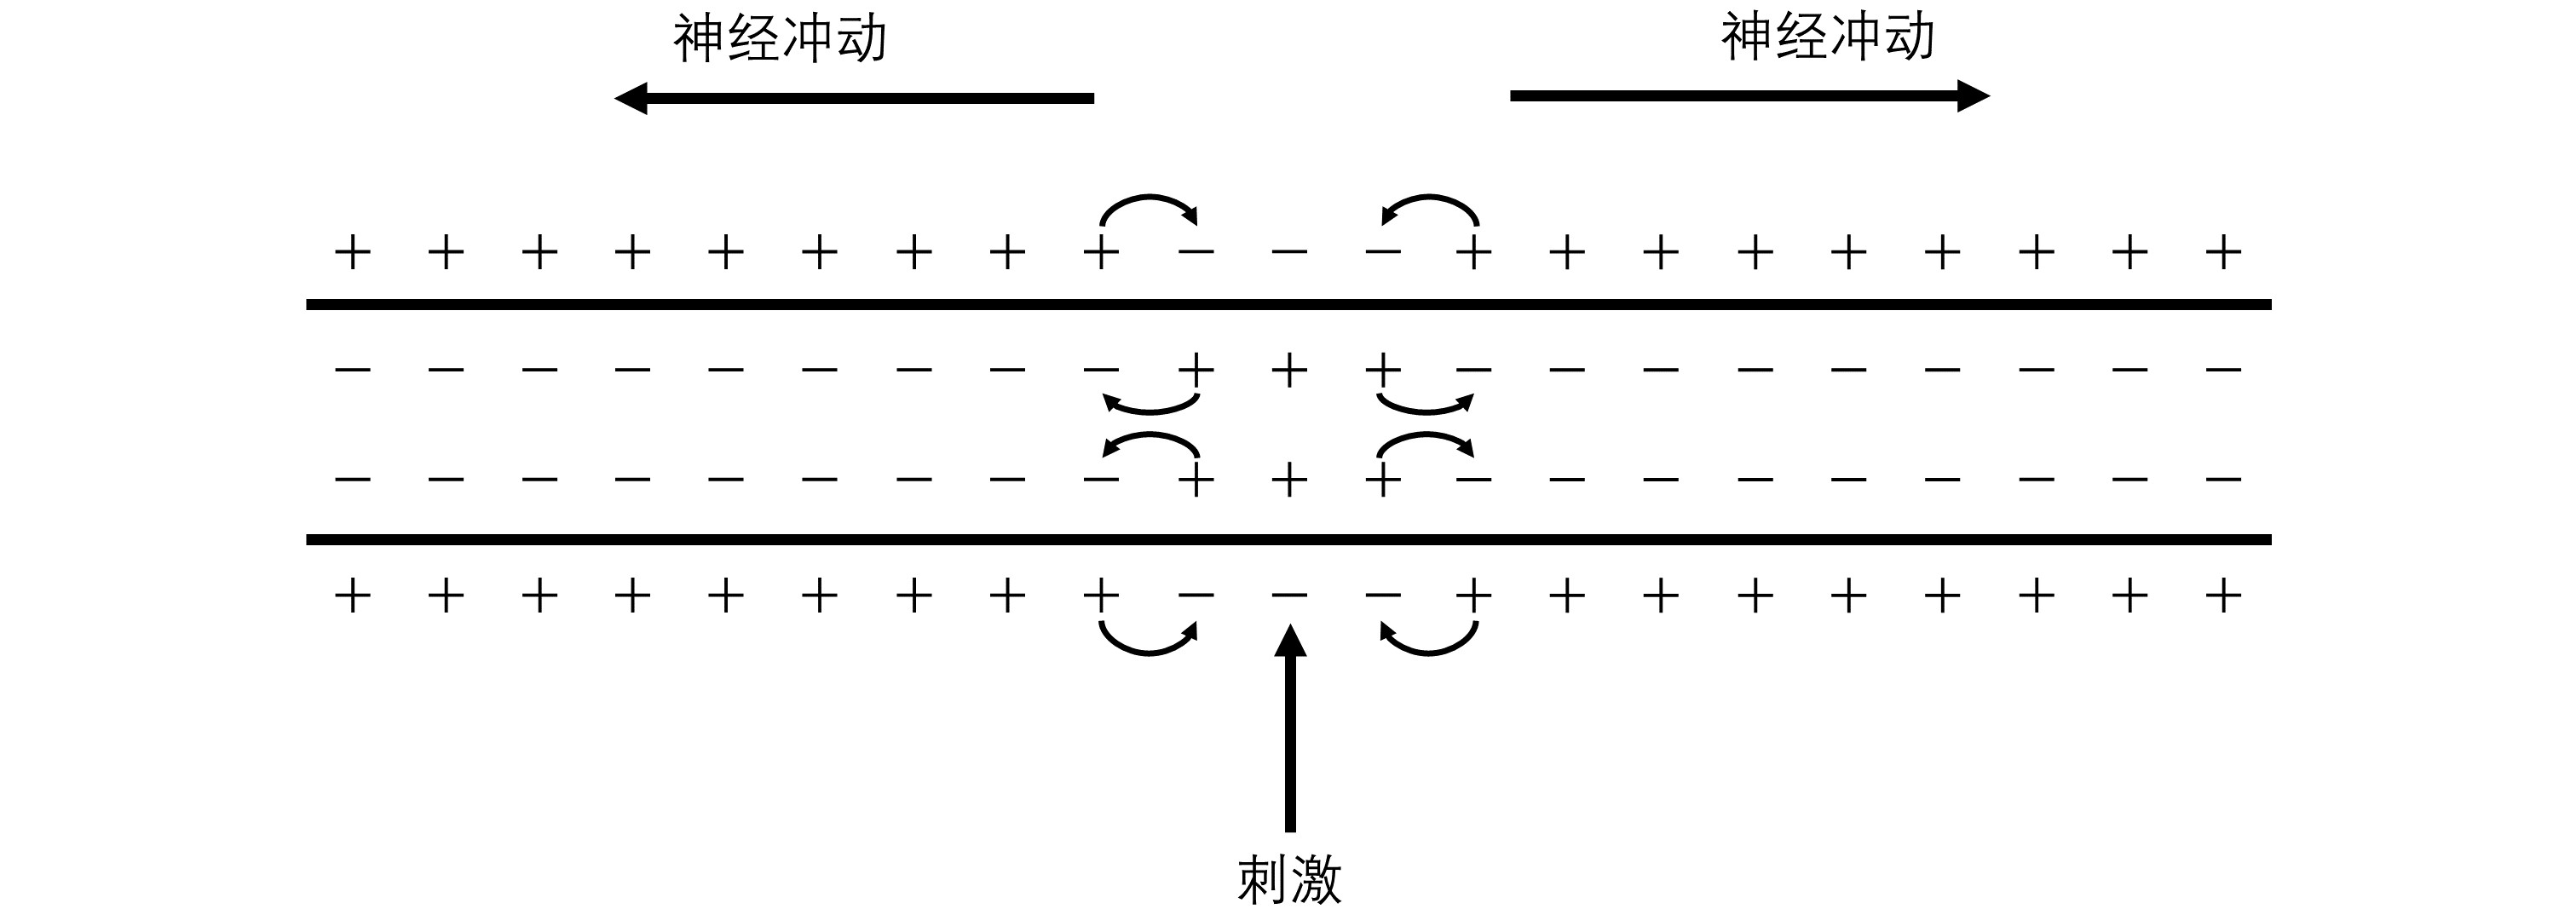
\includegraphics[width=12cm]{BiologyImage/14.jpg}
            \caption{神经冲动传导}
        \end{center}
    \end{figure}\\
    当受到刺激时,膜外的~\ce{Na+}离子大量内流,使局部的电位发生翻转,
    由静息电位变为动作电位,产生了神经冲动,兴奋区域与临近区域存在电位差,
    使得兴奋沿神经纤维推进。\\[2mm]
    信息在神经元上是以电信号的方式传递的,同时这种传递是单向的。
    
\newpage

\subsubsection{突触传递}
    神经元以轴突于其他神经元的树突或细胞体接触,相接触部分称为突触。\\[3mm]
    突触分为三部分:突触前膜,突触后膜,突触间隙。\\[3mm]
    突触前膜:靠近轴突一侧的细胞膜。\\[3mm]
    突触后膜:靠近树突一侧的细胞膜。\\[3mm]
    突触间隙:前膜和后膜之间的空隙。\\[3mm]
    突触传递示意图:
    \begin{figure}[h]
        \begin{center}
            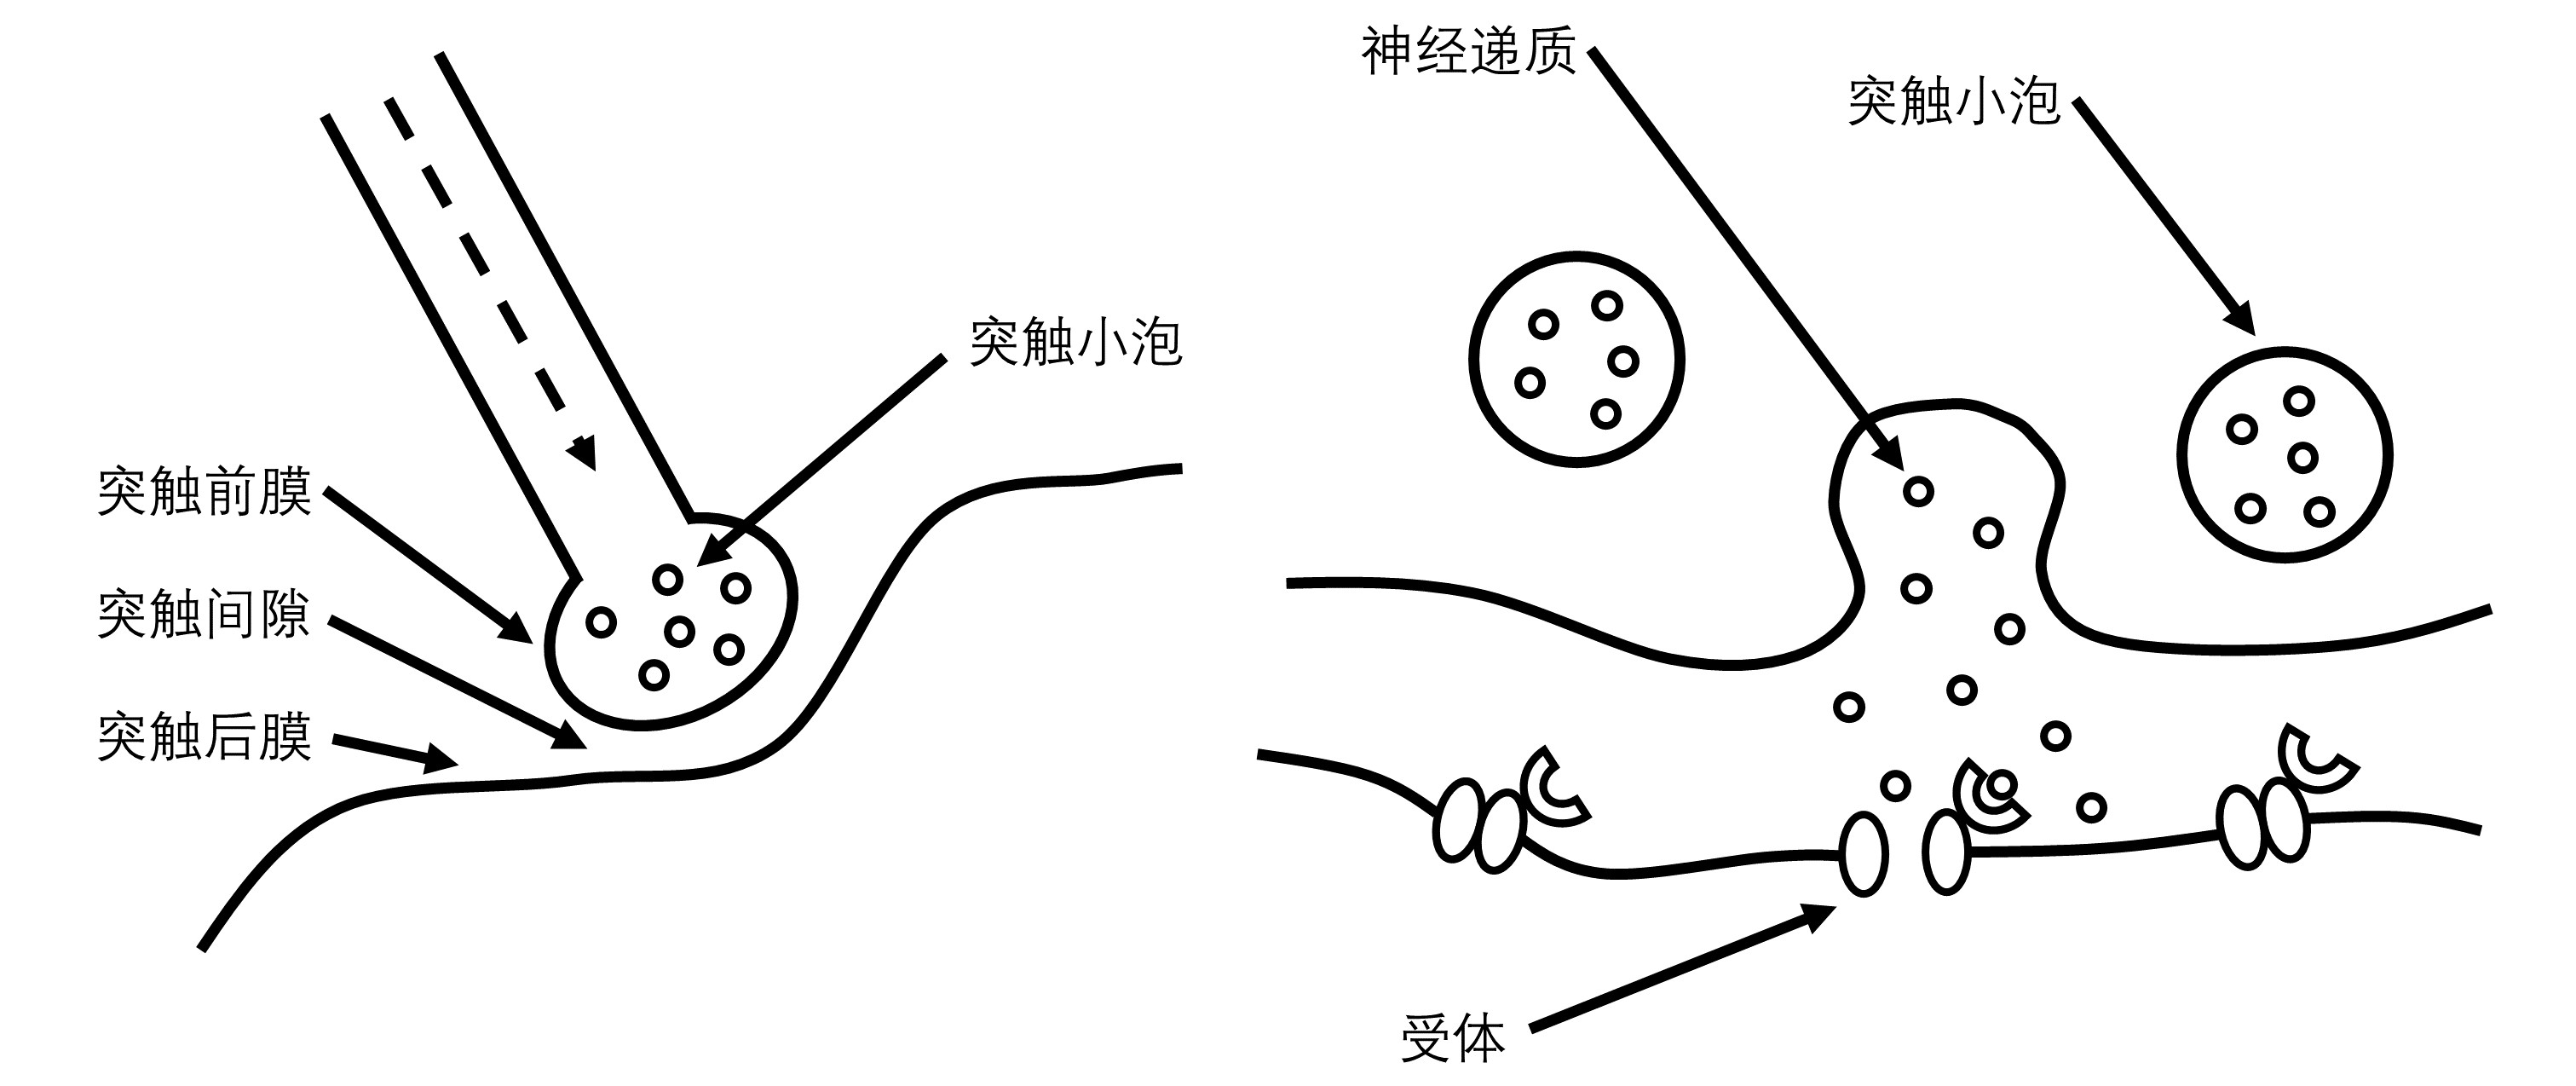
\includegraphics[width=12cm]{BiologyImage/15.jpg}
            \caption{突触传递}
        \end{center}
    \end{figure}\\
    当神经冲动抵达突触前膜时,促使轴突中的突触小泡与突触前膜结合,
    释放其所包含的化学物质到突触间隙,这种化学物质被称为神经递质,
    神经递质会与突触后膜上的受体结合,引发神经后膜上的神经冲动。
    随后多余的神经递质就会被突触间隙中的酶降解失活。\\[2mm]
    信息在神经元间是以化学物质的方式传递的,同时这种传递是单向的。

\subsubsection{低级神经中枢-脊髓}
    人类的低级神经中枢是脊髓。\\[3mm]
    人类的脊髓呈长管状,位于脊柱的椎管内,上端与延髓相连接。\\[3mm]
    脊髓的外周的脊髓白质,由神经纤维构成。\\[3mm]
    脊髓的内部是脊髓灰质,由神经元细胞体构成。\\[6mm]
    非条件反射指的是以脊髓为中枢的反射活动,通常是与生俱来的,较为简单。\\[3mm]
    虽然脊髓调节的活动简单,但是脊髓调节反应速度快,有助于迅速避开危险。

\newpage

\subsubsection{高级神经中枢-脑}
    人类的高级神经中枢的脑。\\[3mm]
    人类的脑可以分为六个部分:大脑,小脑,间脑,中脑,脑桥,延髓。\\[3mm]
    大脑是脑中最为发达的部分,大脑由两个大脑半球组成。\\[3mm]
    大脑的外周是大脑灰质,由神经元细胞体组成。\\[3mm]
    大脑的内部是大脑白质,由神经纤维组成。\\[3mm]
    大脑外周的灰质也被称为大脑皮质。\\[6mm]
    条件反射指的是以大脑为中枢的反射活动,通常是后天形成的,较为复杂。\\[3mm]
    虽然大脑调节反应速度慢,但是大脑调节的活动复杂,有助于解决复杂问题。

\subsubsection{自主神经}
    我们将不受人的意志支配的神经,称为自主神经,例如心跳的跳动,例如胃肠的蠕动。\\[3mm]
    人类的自主神经分为两部分:交感神经和副交感神经。\\[3mm]
    当人精神紧张时,交感神经兴奋,心跳加快,血压增高,血糖上升,胃肠蠕动减缓。\\[3mm]
    当人精神放松时,副交感神经兴奋,心跳减缓,血压下降,血糖下降,胃肠蠕动加快。\\

\subsection{内分泌系统}
    内分泌系统由内分泌腺组成。\\[3mm]
    内分泌腺指的是没有分泌管的腺体,其分泌的物质直接进入周围的血管或淋巴管。\\[3mm]
    内分泌腺分泌的物质被称为激素,激素的量非常少,但作用却非常显著。\\[6mm]
    以下表格列举了下丘脑分泌的激素:\vspace{5pt}
    \begin{table}[h]
        \begin{center}
            \begin{tabular}{l|l|l|l}
                \hline
                激素名称\qquad\qquad&本质\qquad\qquad&作用部位\qquad\qquad&生理作用\qquad\qquad\\ \hline
                促甲状腺激素释放激素&多肽&垂体&促进垂体分泌促甲状腺激素\\ \hline
                促生殖腺激素释放激素&多肽&垂体&促进垂体分泌促生殖腺激素\\ \hline
                促肾上腺皮质激素释放激素\qquad\qquad&多肽&垂体&促进垂体分泌促肾上腺皮质激素\\ \hline
                抗利尿激素&多肽&肾小管&促进肾小管对水的重吸收作用\\ \hline
            \end{tabular}
            \caption{下丘脑分泌的激素}
        \end{center}
    \end{table}

\newpage

    以下表格列举了垂体分泌的激素:\vspace{5pt}
    \begin{table}[h]
        \begin{center}
            \begin{tabular}{l|l|l|l}
                \hline
                激素名称\qquad\qquad&本质\qquad\qquad&作用部位\qquad\qquad&生理作用\qquad\qquad\\ \hline
                促甲状腺激素&蛋白质&甲状腺&促进甲状腺分泌甲状腺素\\ \hline
                促生殖腺激素&蛋白质&生殖腺&促进生殖腺分泌性激素\\ \hline
                促肾上腺皮质激素\qquad\qquad&蛋白质&肾上腺&促进肾上腺分泌肾上腺皮质激素\\ \hline
                生长激素&蛋白质&全身&促进蛋白质的合成和骨骼的生长\\ \hline
            \end{tabular}
            \caption{垂体分泌的激素}
        \end{center}
    \end{table}\\
    以下表格列举了甲状腺分泌的激素:\vspace{5pt}
    \begin{table}[h]
        \begin{center}
            \begin{tabular}{l|l|l|l}
                \hline
                激素名称\qquad\qquad&本质\qquad\qquad&作用部位\qquad\qquad&生理作用\qquad\qquad\\ \hline
                甲状腺素&氨基酸衍生物&全身&促进新陈代谢和生长发育\\ \hline
            \end{tabular}
            \caption{甲状腺分泌的激素}
        \end{center}
    \end{table}\\
    以下表格列举了肾上腺分泌的激素:\vspace{5pt}
    \begin{table}[h!]
        \begin{center}
            \begin{tabular}{l|l|l|l}
                \hline
                激素名称\qquad\qquad&本质\qquad\qquad&作用部位\qquad\qquad&生理作用\qquad\qquad\\ \hline
                肾上腺素&氨基酸衍生物&全身&促进新陈代谢和肝糖原分解\\ \hline
                肾上腺皮质激素&固醇&肾脏&调节盐和糖的代谢和血液中的水分\\ \hline
            \end{tabular}
            \caption{肾上腺分泌的激素}
        \end{center}
    \end{table}\\
    以下表格列举了胰岛分泌的激素:\vspace{5pt}
    \begin{table}[h!]
        \begin{center}
            \begin{tabular}{l|l|l|l}
                \hline
                激素名称\qquad\qquad&本质\qquad\qquad&作用部位\qquad\qquad&生理作用\qquad\qquad\\ \hline
                胰岛素&蛋白质&全身&降低血糖浓度,促进组织细胞利用血糖\\ \hline
                胰高血糖素&蛋白质&肝脏&升高血糖浓度,促进肝糖原分解\\ \hline
            \end{tabular}
            \caption{胰岛分泌的激素}
        \end{center}
    \end{table}\\
    以下表格列举了生殖腺分泌的激素:\vspace{5pt}
    \begin{table}[h!]
        \begin{center}
            \begin{tabular}{l|l|l|l}
                \hline
                激素名称\qquad\qquad&本质\qquad\qquad&作用部位\qquad\qquad&生理作用\qquad\qquad\\ \hline
                雄激素&固醇&全身&促进雄性生殖器官的发育和精子的形成\\ \hline
                雌激素&固醇&全身&促进雌性生殖器官的发育和卵子的形成\\ \hline
            \end{tabular}
            \caption{生殖腺分泌的激素}
        \end{center}
    \end{table}

\newpage

\subsection{免疫系统}
    细胞可以通过细胞膜上的糖蛋白和糖脂进行细胞识别。\\[3mm]
    抗原指的是所有被生物体细胞识别为异己物质并受免疫反应排斥的物质。\\[3mm]
    抗原大多数是外源性的,例如病原体或异体的组织细胞。\\[3mm]
    抗原少部分是内源性的,例如癌细胞或衰老的组织细胞。

\subsubsection{非特异性免疫}
    非特异性免疫是先天形成的,是人类在长期进化中形成并通过遗传巩固下来的天然免疫功能。\\[2mm]
    非特异性免疫不具有针对性,对各类病原体都有一定防御作用。\\[3mm]
    人体的第一道防线是机体完整的皮肤和黏膜组成的物理屏障。\\[3mm]
    皮肤和粘膜同时还可以分泌一些化学物质,也能阻挡病原体的入侵,
    例如汗液中的酸性分泌物,例如皮肤腺分泌的不饱和脂肪酸,例如胃黏膜分泌的胃酸,均具有杀菌效果。\\[3mm]
    皮肤和粘膜表面通常还生活者一定数量的菌群,它们一般情况下并不致病,
    但是对其他的病原微生物具有拮抗作用,例如口腔中的链球菌可以产生过氧化氢对白喉杆菌有抑制作用。\\[3mm]
    人体的第二道防线是巨噬细胞的吞噬作用。\\[3mm]
    巨噬细胞可以伸出伪足吞噬进入结缔组织的病原体,纳入细胞质内形成吞噬泡,溶酶体随即与吞噬泡融合,
    溶酶体中含有溶菌酶和蛋白水解酶,可以杀灭病原体并将其消化。

\subsubsection{特异性免疫}
    特异性免疫是后天形成的,是淋巴细胞与特定抗原接触后才形成的免疫功能。\\[2mm]
    特异性免疫具有针对性,只对特定的抗原具有防御作用。\\[3mm]
    人体的第三道防线是淋巴细胞的特异性识别。\\[4mm]
    B淋巴细胞主导的免疫反应称为体液免疫,受到刺激时可以分化出效应B细胞和记忆B细胞。\\[2mm]
    效应B细胞可以通过分泌抗体,直接杀死病原体或促使巨噬细胞吞噬病原体。\\[2mm]
    记忆B细胞则具有记忆作用,当再次遇到相同病原体入侵时,可以更快的分化出效应B细胞。\\[4mm]
    T淋巴细胞主导的免疫反应称为细胞免疫,受到刺激时可以分化出致敏T细胞和记忆T细胞。\\[2mm]
    致敏B细胞即可以分泌淋巴因子杀死抗原细胞,也可以通过密切接触杀死抗原细胞。\\[2mm]
    记忆T细胞则具有记忆作用,当再次遇到相同病原体入侵时,可以更快的分化出致敏T细胞。\\[4mm]
    效应B细胞通常也称作浆细胞,其具有丰富的内质网,可以支持其分泌免疫球蛋白,即抗体。

\newpage

\subsection{植物生长素}
    生长素是一种植物激素,可以促进植物生长。\\[3mm]
    生长素通常分泌于植物生长活跃的部位:茎尖,根尖,嫩叶,发育中的种子。\\[3mm]
    生长素分泌后会转运到其他部位调节生长发育:由茎尖转运到茎,由根尖转运到根。\\[6mm]
    当生长素的浓度低于最适浓度时,随着生长素浓度的增加,对植物的促进作用增加。\\[3mm]
    当生长素的浓度高于最适浓度时,随着生长素浓度的增加,对植物的促进作用减弱。\\[6mm]
    生长素浓度对植物生长的影响:
    \begin{figure}[h]
        \begin{center}
            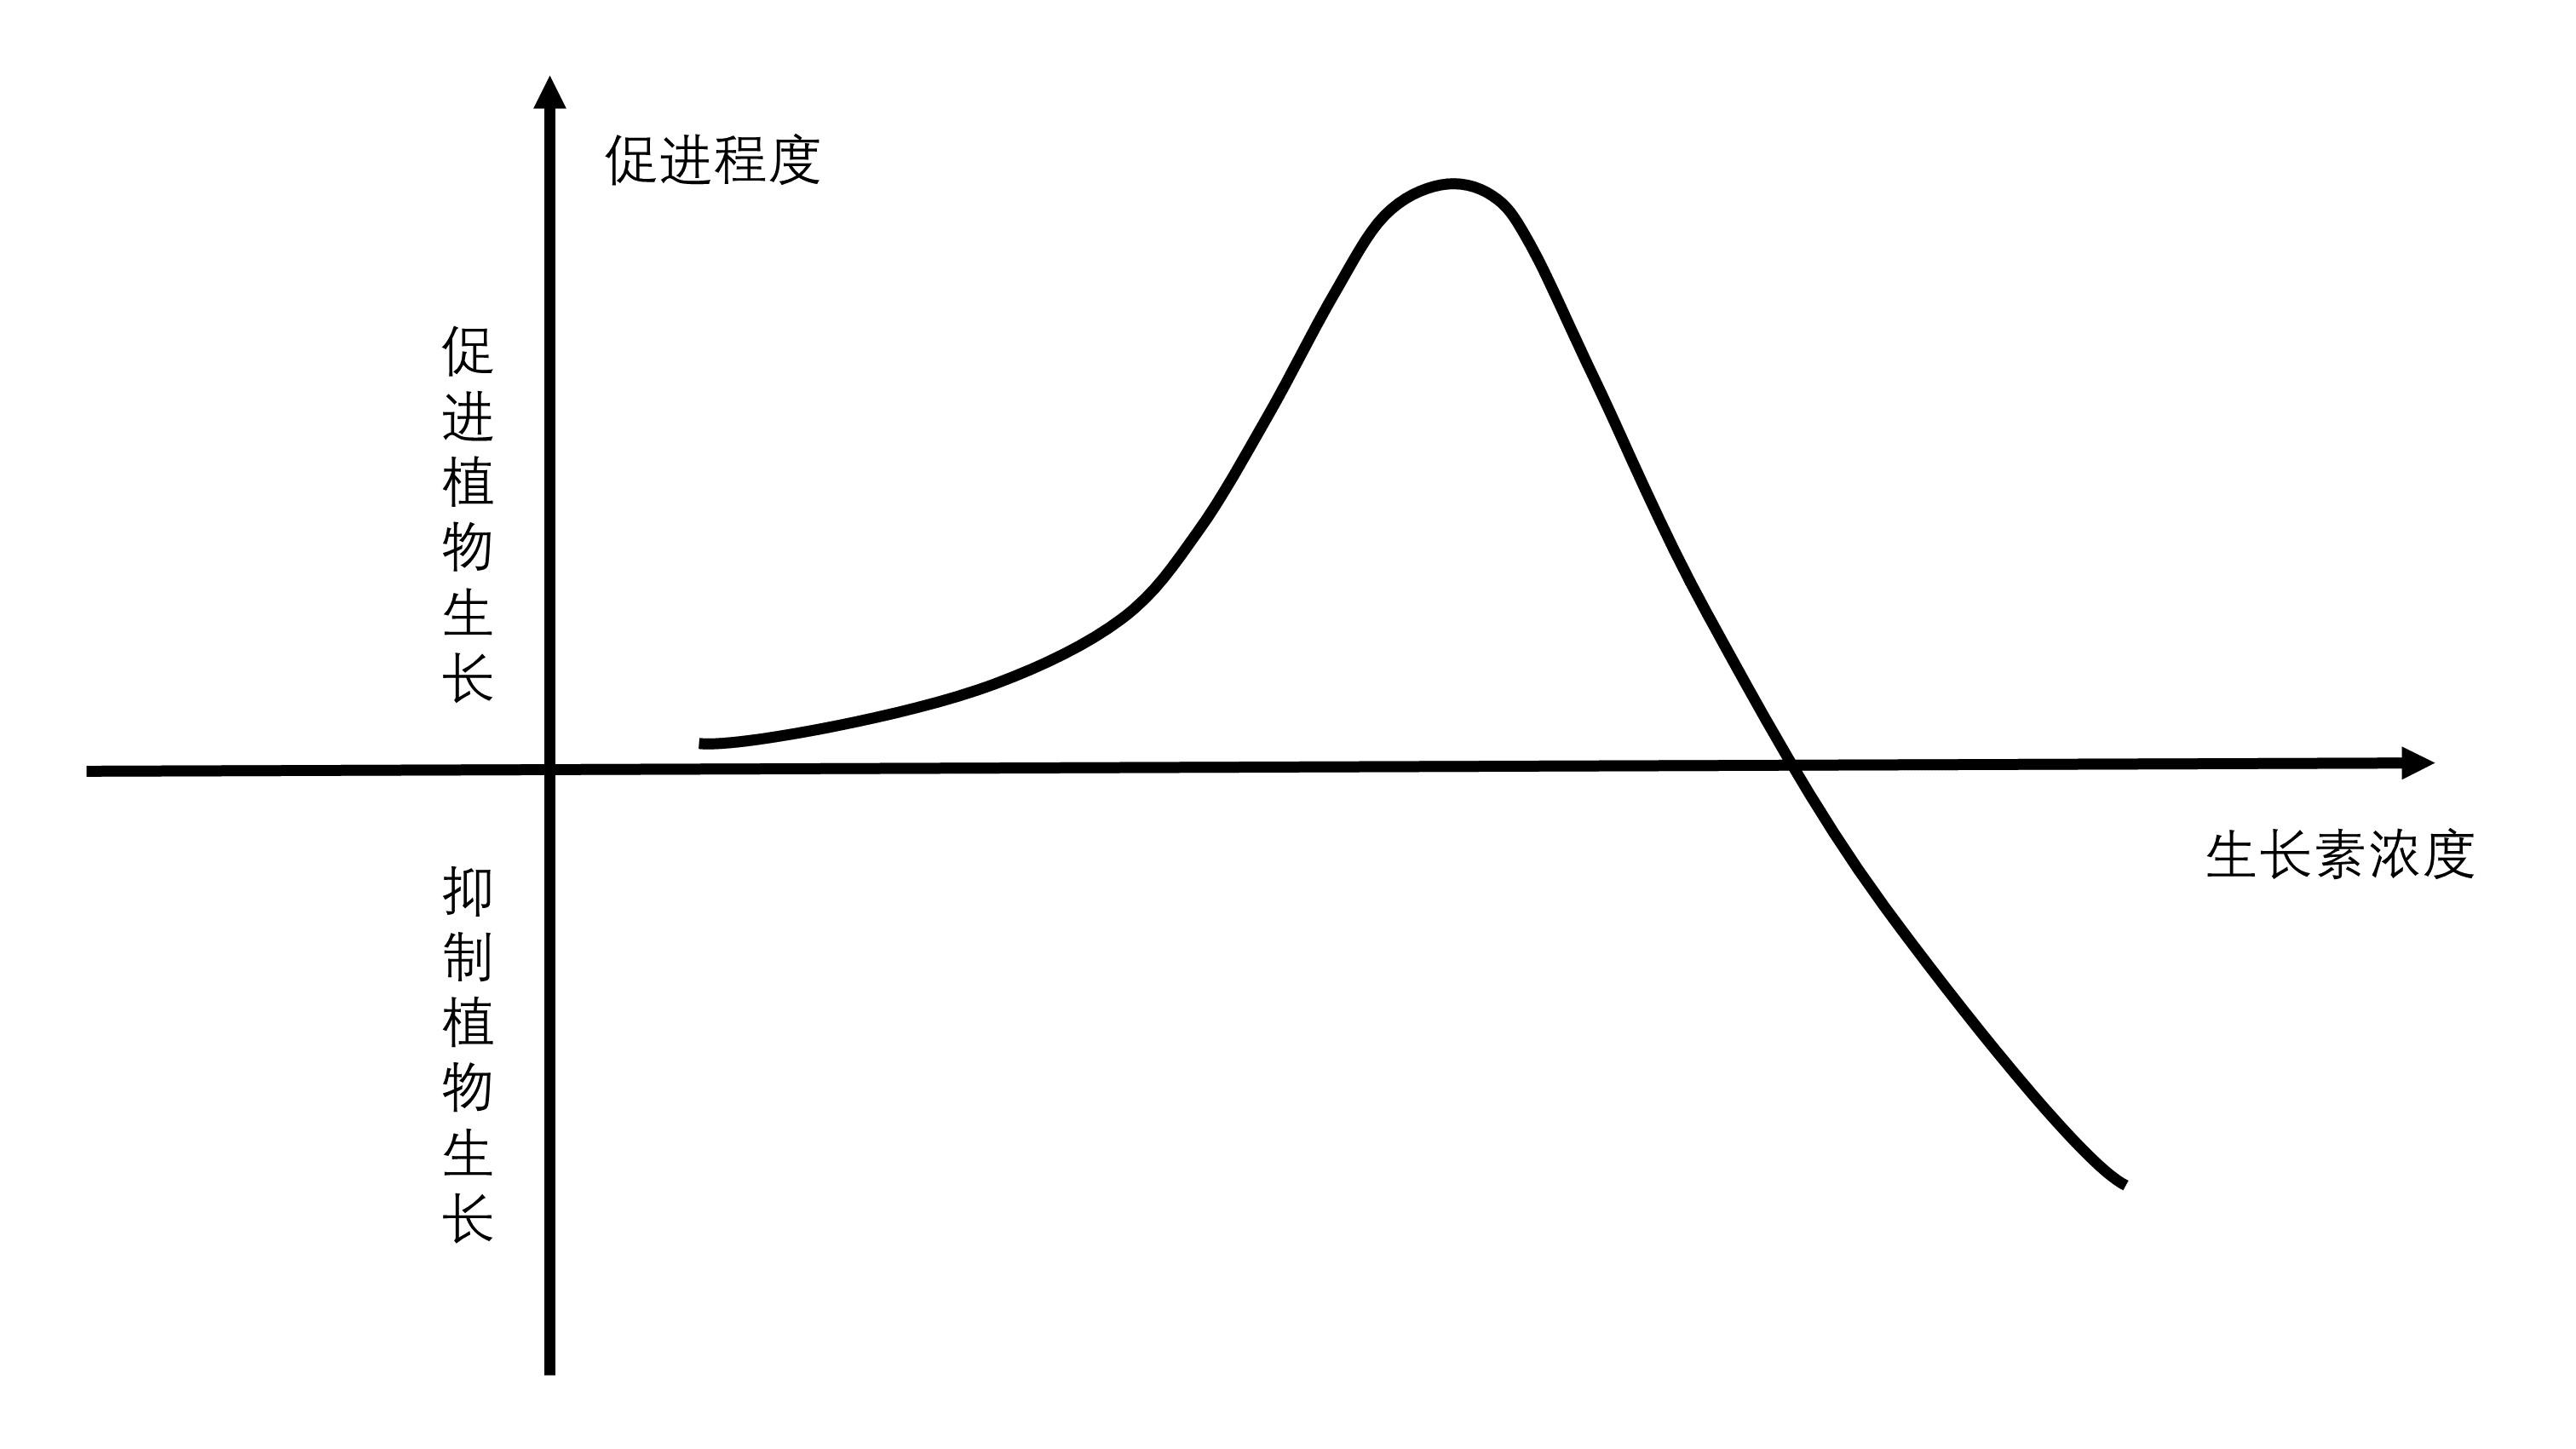
\includegraphics[width=10cm]{BiologyImage/16.jpg}
            \caption{生长素浓度对植物生长的影响}
        \end{center}
    \end{figure}\\
    生长素的运输有两种方式:横向运输和纵向运输。\\[3mm]
    横向运输发生在生长素产生的部位内,例如茎尖和根尖。\\[3mm]
    纵向运输发生在生长素产生的部位外,例如茎和根。\\[3mm]
    需要指出的是,此处的横向和纵向均以植物正常生长时的方向为准,与植物实际生长方向无关。\\[6mm]
    横向运输受光照影响,由向光侧往背光侧转运,横向运输受重力影响,由背地侧往向地侧转运。\\[3mm]
    纵向运输不受外界调节影响,茎尖的生长素向下运输,根尖的生长素向上运输。\\[6mm]
    促进植物细胞伸长分裂的植物激素:生长素,赤霉素,细胞分裂素。\\[3mm]
    抑制植物细胞伸长分裂的植物激素:脱落酸,乙烯。\\[3mm]
    生长素的化学本质是吲哚乙酸,类似物质有:吲哚乙酸,吲哚丁酸,萘乙酸,2,4-D。

\newpage

\subsubsection{茎的向光性}
    生长素在茎尖产生,通过横向运输,生长素由向光侧往背光侧运输。\\[3mm]
    生长素在向光侧的量较少,生长素在背光侧的量较多,通过纵向运输,生长素由茎尖转移到茎。\\[3mm]
    由于茎对生长素敏感度较弱,因此生长素浓度低于最适浓度,故背光侧生长较多。\\[3mm]
    由于背光侧生长较多,故茎整体向光弯曲,这就是茎的向光性。
    \begin{figure}[h]
        \begin{center}
            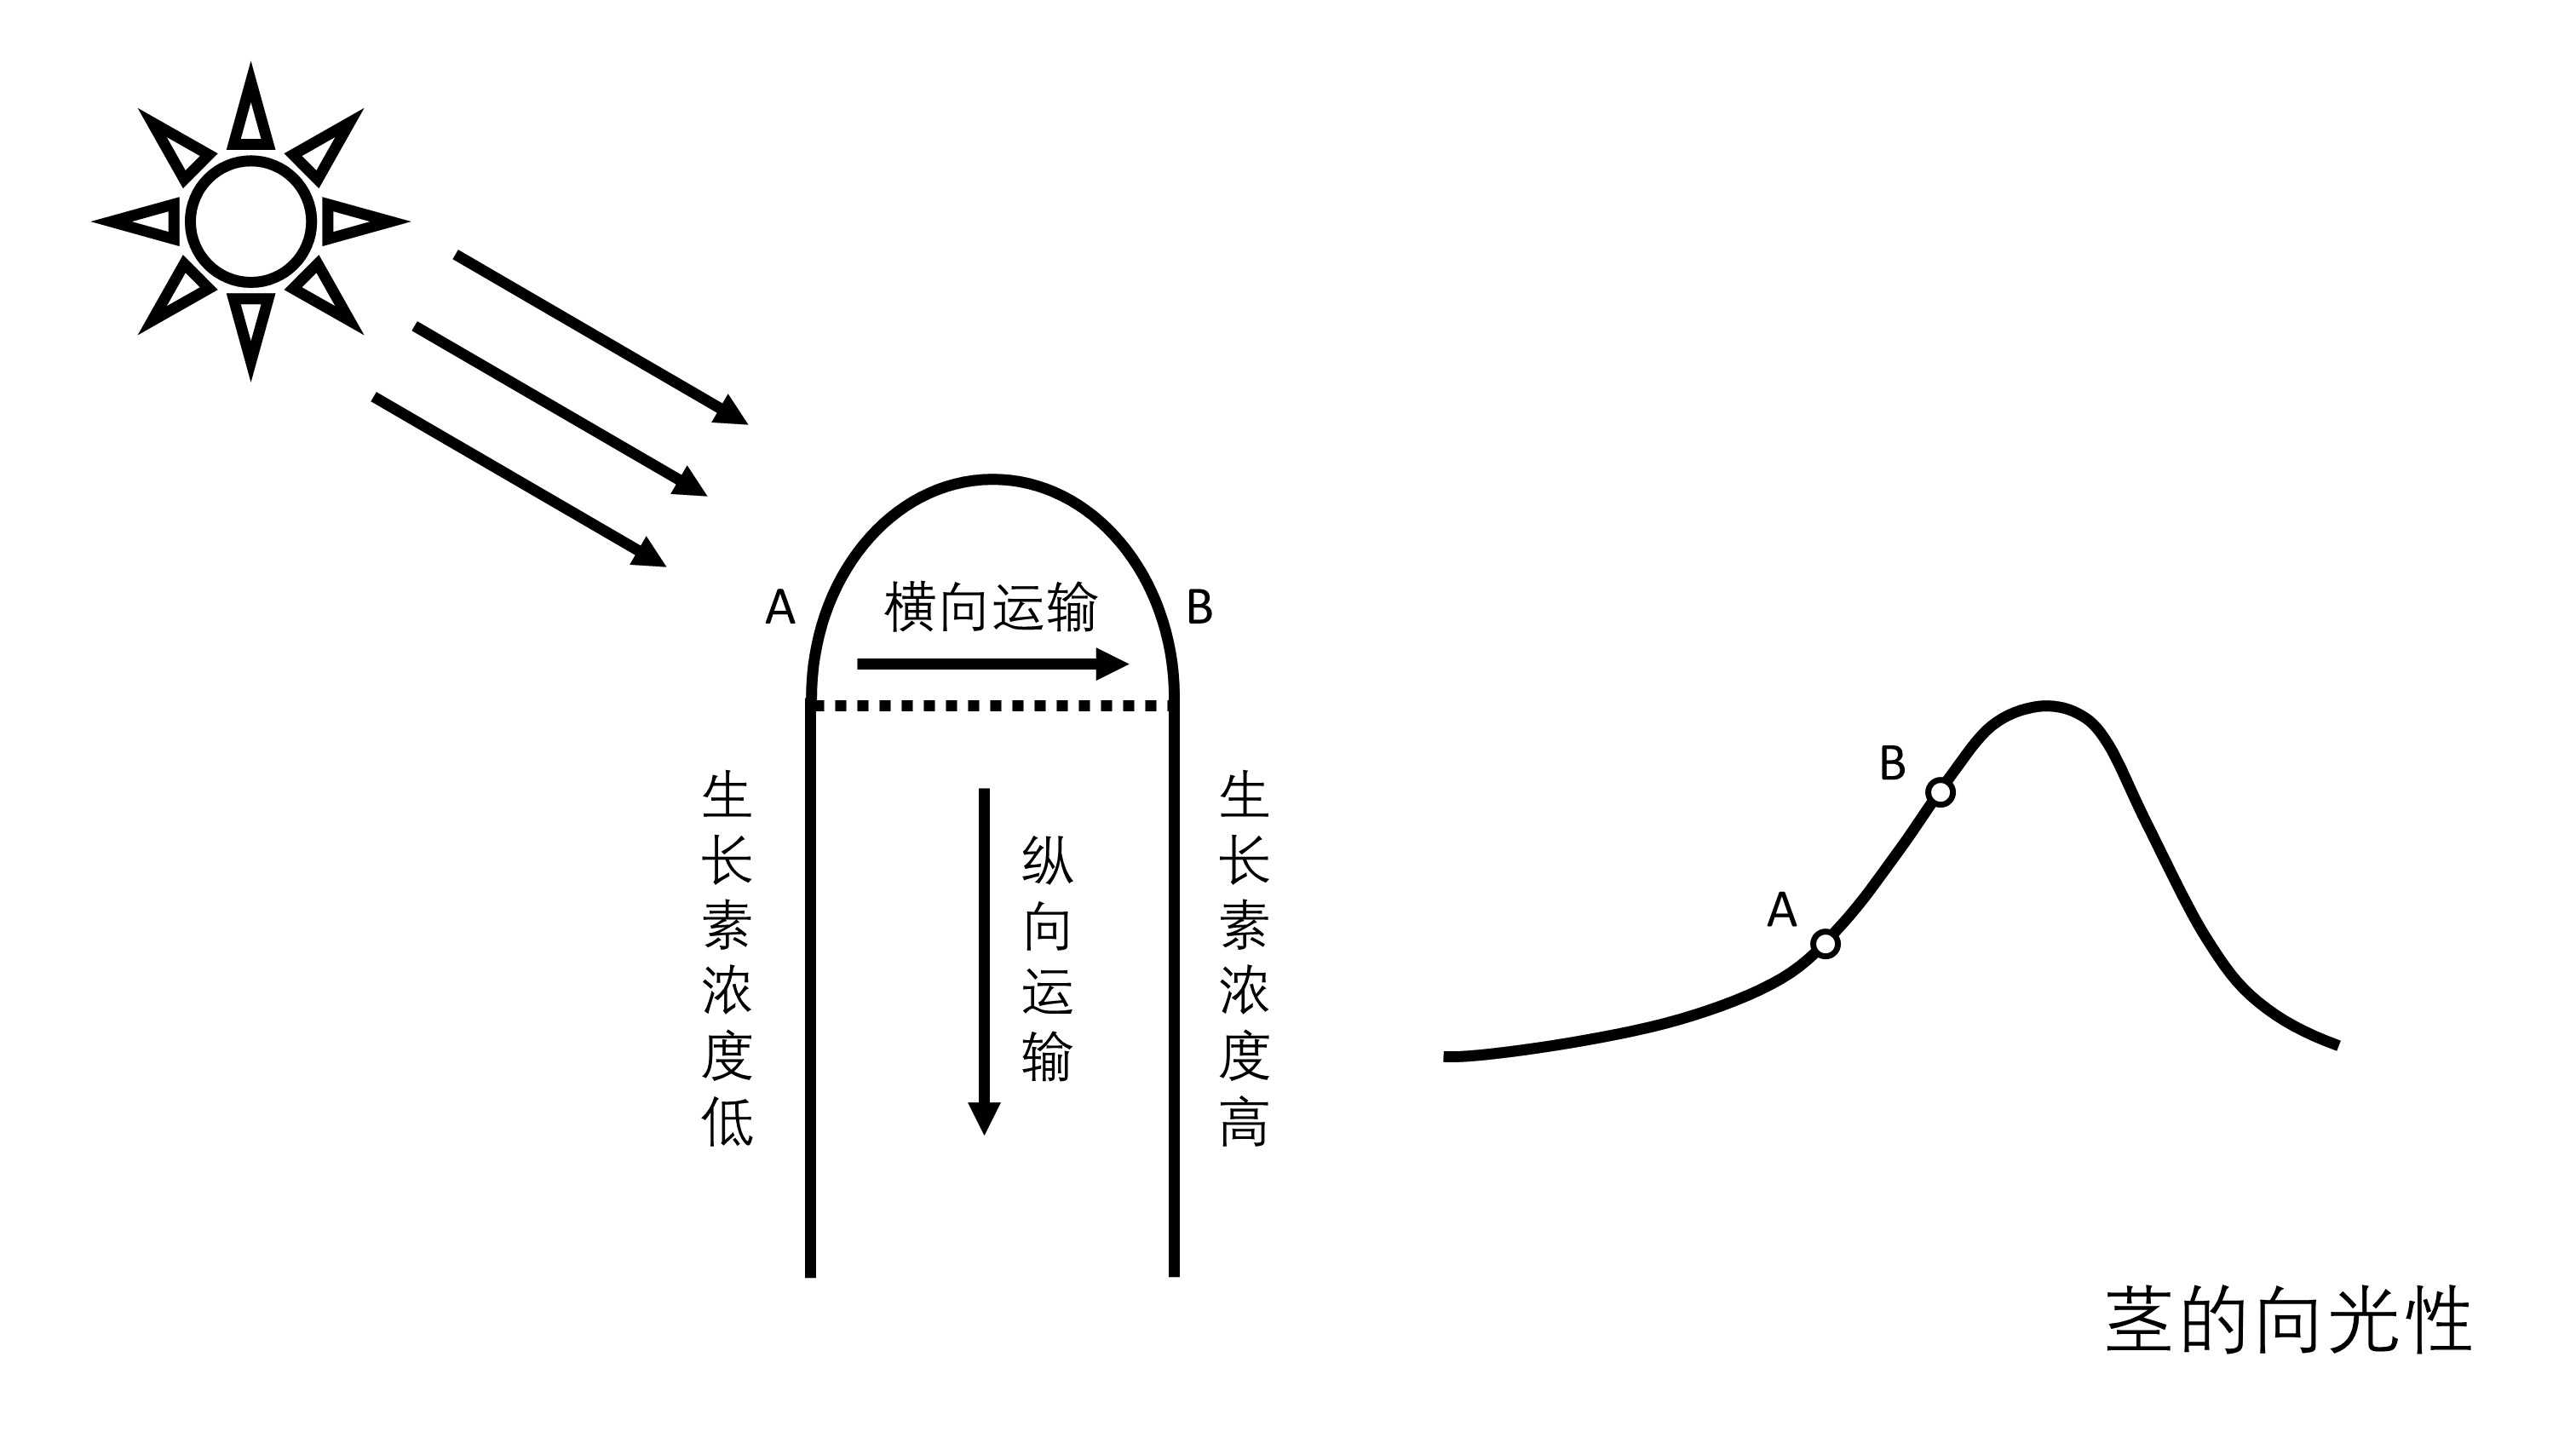
\includegraphics[width=10cm]{BiologyImage/17.jpg}
            \caption{茎的向光性}
        \end{center}
    \end{figure}\vspace{-25pt}

\subsubsection{根的背光性}
    生长素在根尖产生,通过横向运输,生长素由向光侧往背光侧运输。\\[3mm]
    生长素在向光侧的量较少,生长素在背光侧的量较多,通过纵向运输,生长素由根尖转移到根。\\[3mm]
    由于根对生长素敏感度较强,因此生长素浓度高于最适浓度,故向光侧生长较多。\\[3mm]
    由于向光侧生长较多,故茎整体背光弯曲,这就是根的背光性。
    \begin{figure}[h]
        \begin{center}
            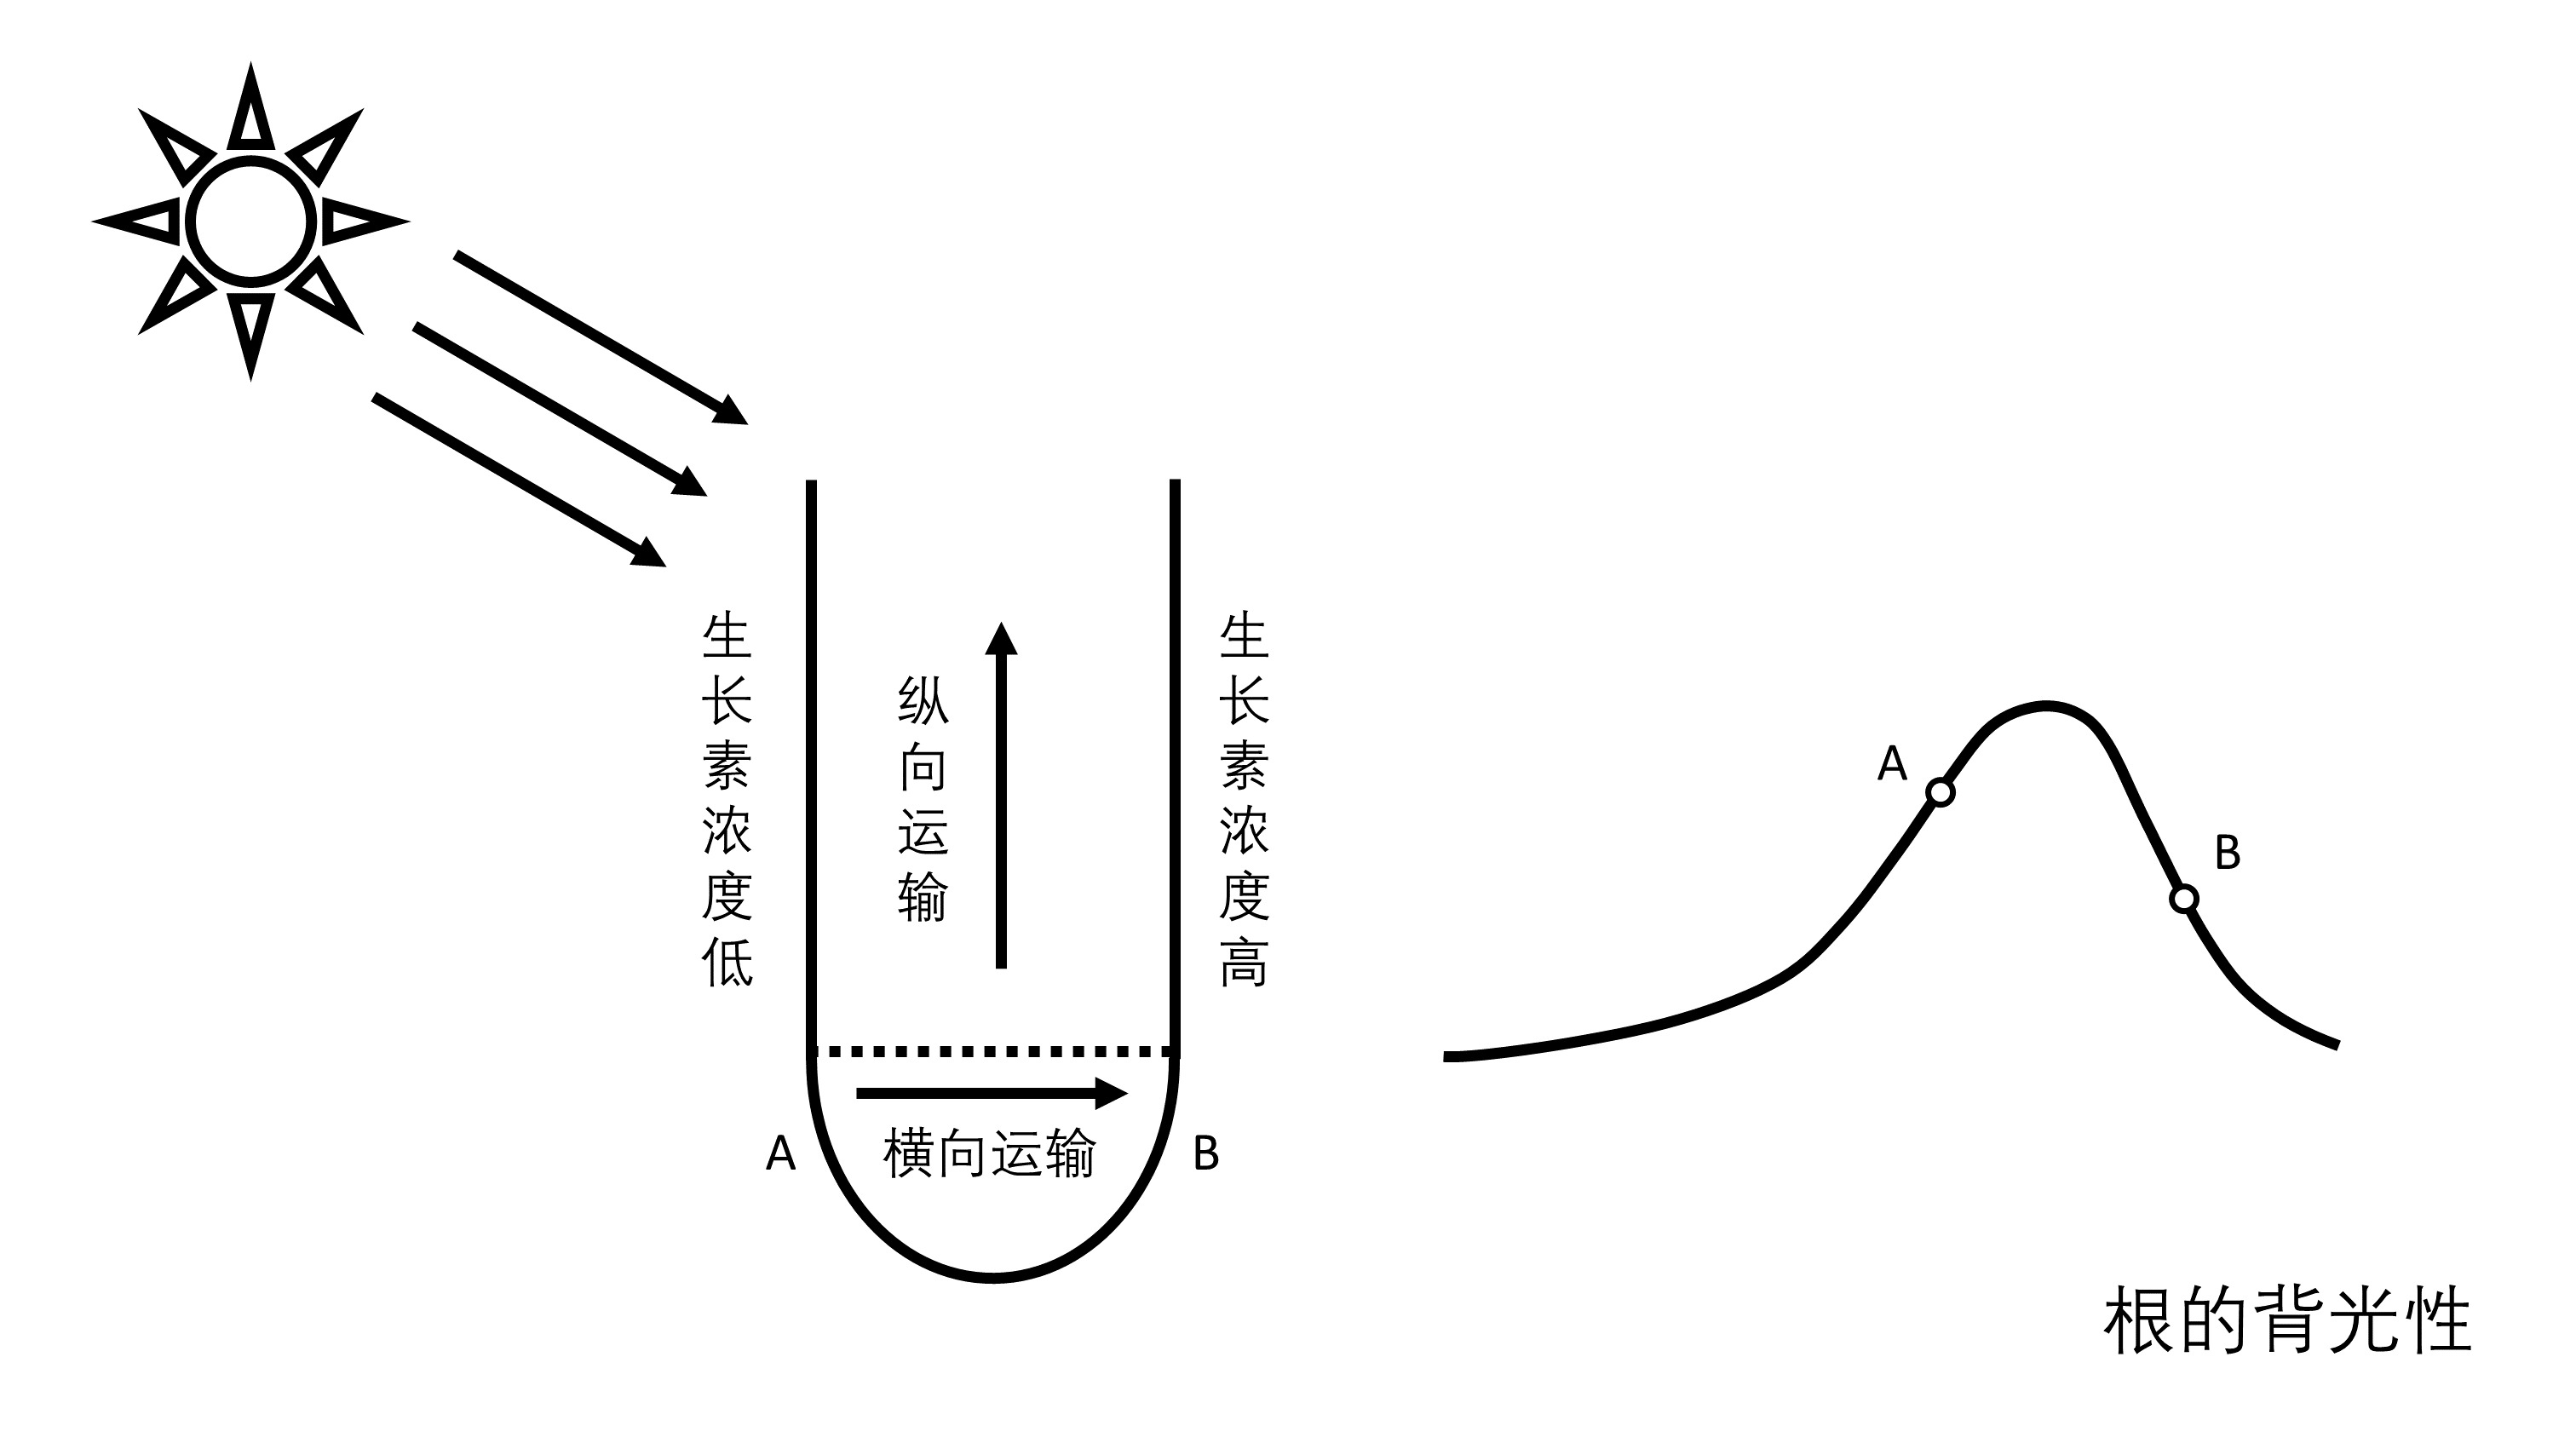
\includegraphics[width=10cm]{BiologyImage/18.jpg}
            \caption{根的背光性}
        \end{center}
    \end{figure}

\newpage

\subsubsection{茎的背地性}
    生长素在茎尖产生,通过横向运输,生长素由背地侧往向地侧运输。\\[3mm]
    生长素在向地侧的量较多,生长素在背地侧的量较少,通过纵向运输,生长素由茎尖转移到茎。\\[3mm]
    由于茎对生长素敏感度较弱,因此生长素浓度低于最适浓度,故向地侧生长较多。\\[3mm]
    由于向地侧生长较多,故茎整体背地弯曲,这就是茎的背地性。
    \begin{figure}[h]
        \begin{center}
            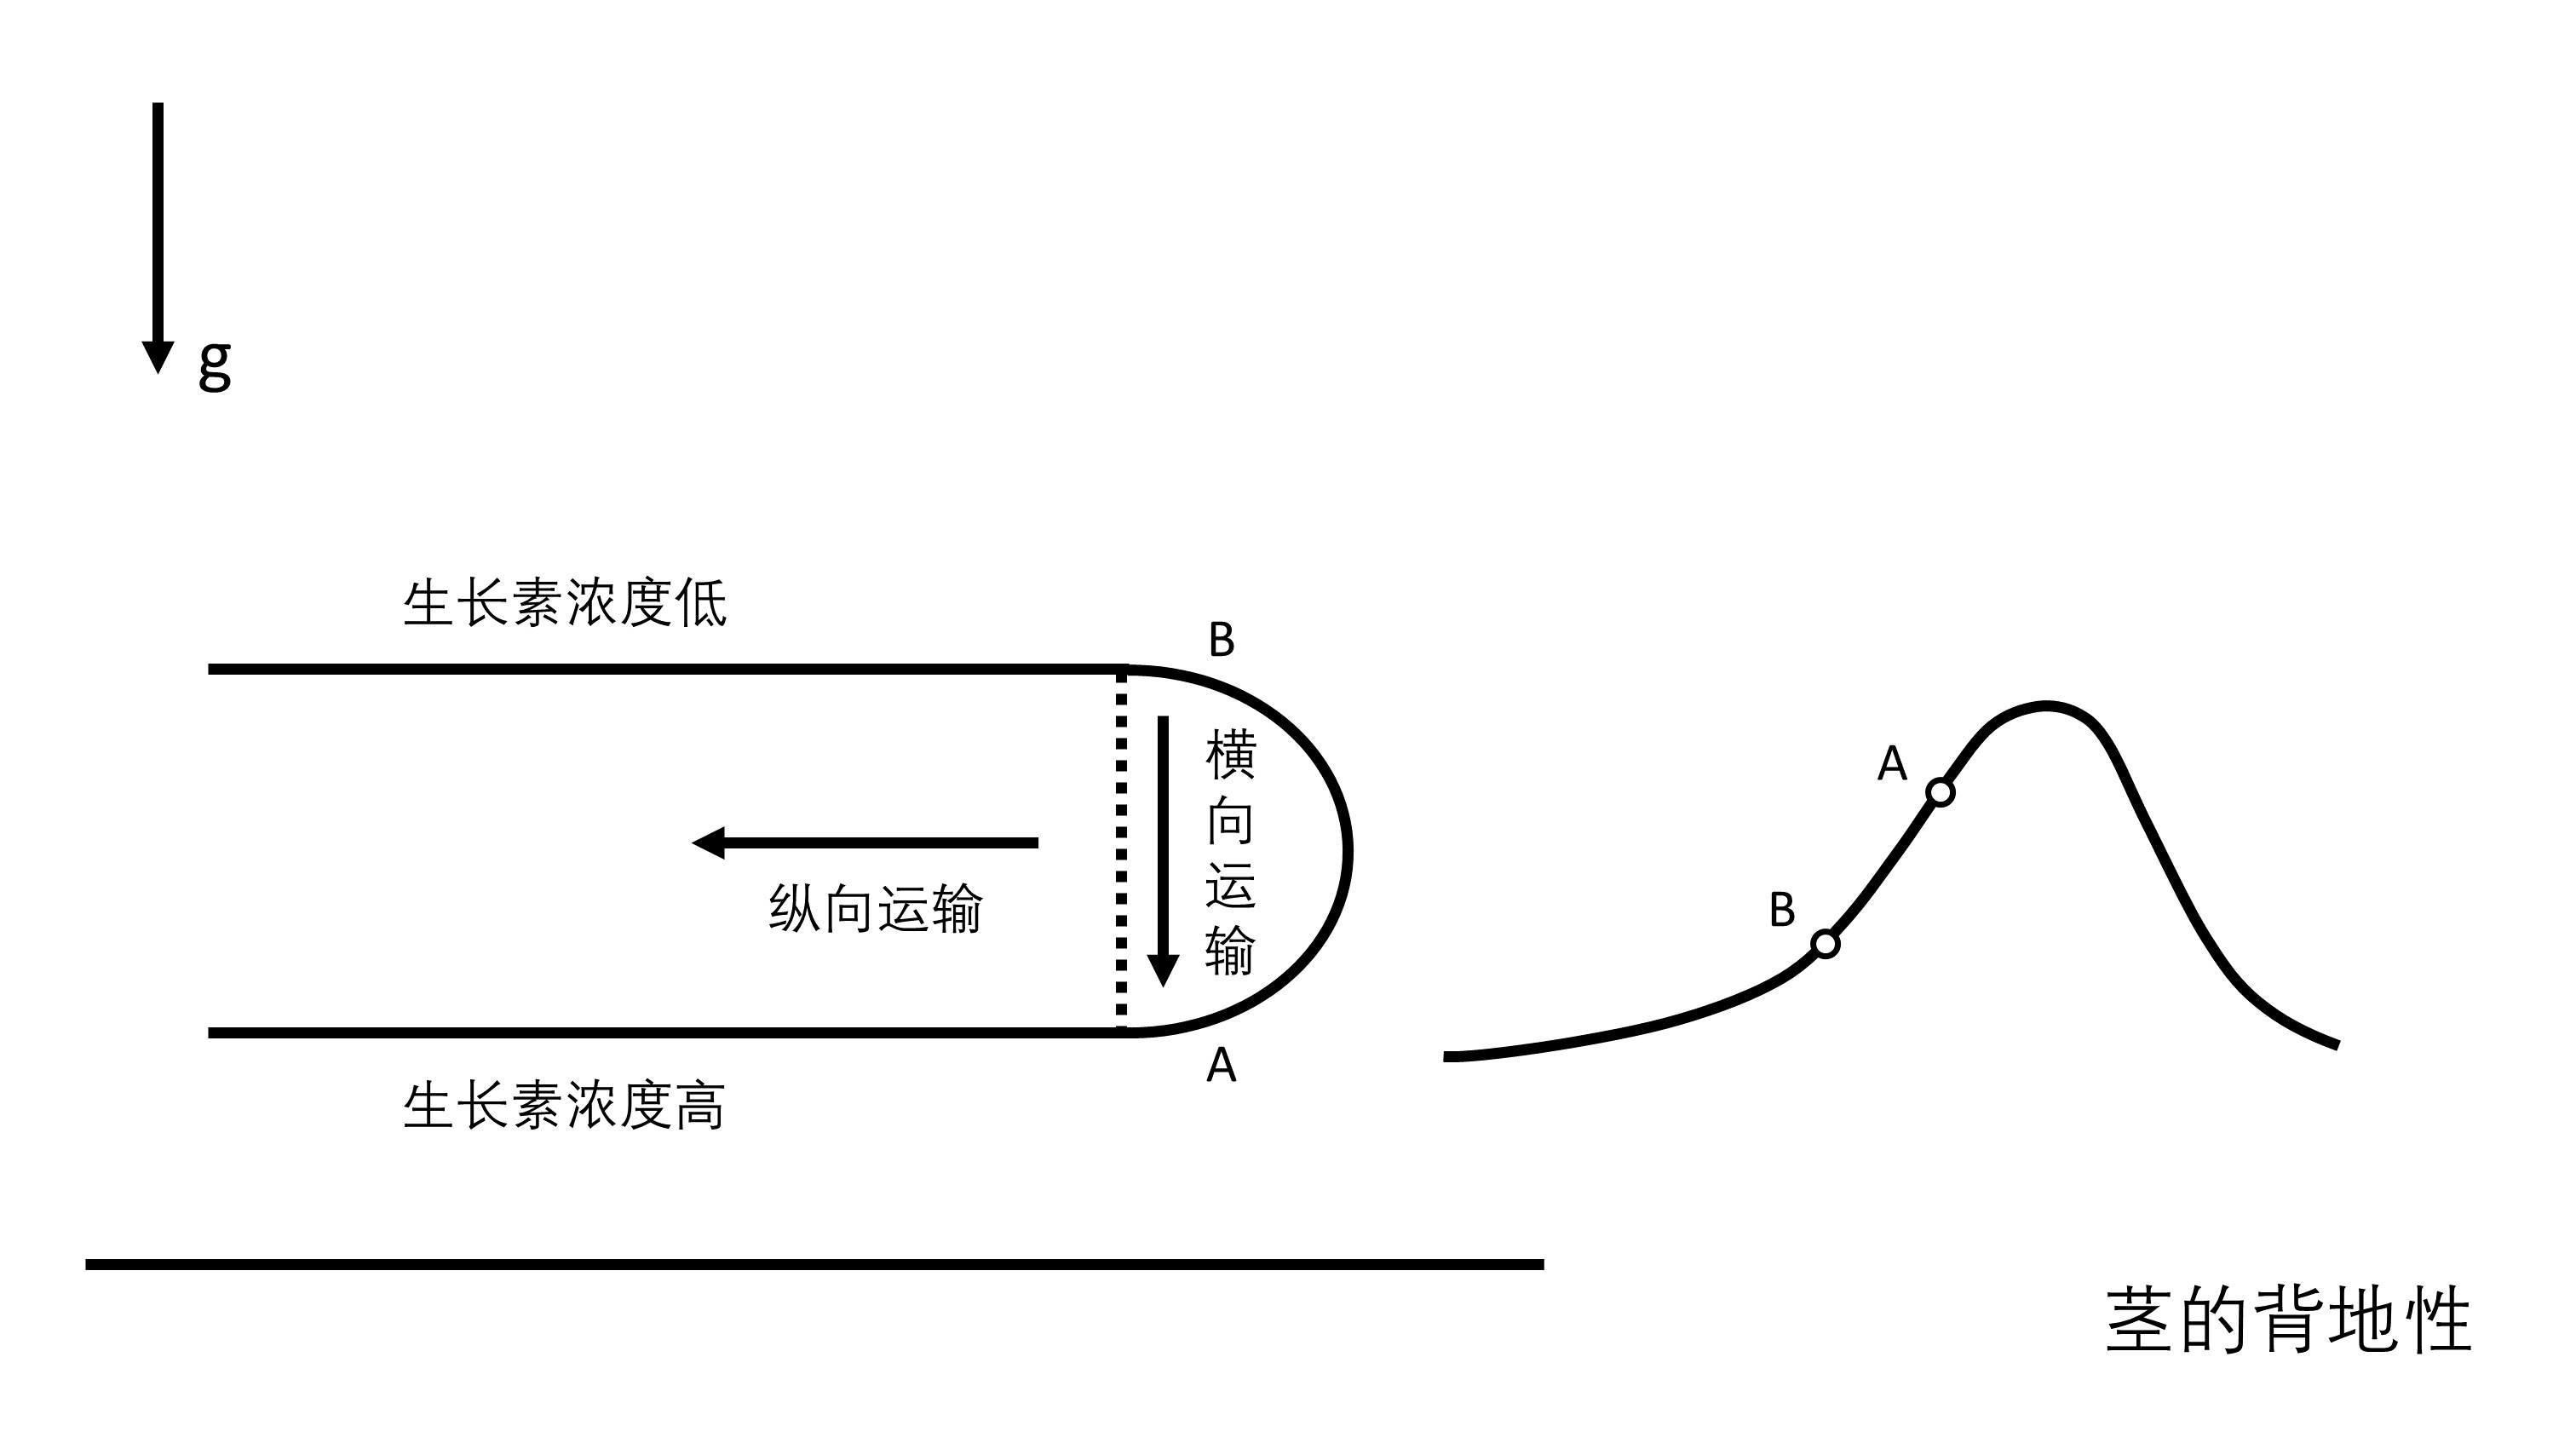
\includegraphics[width=10cm]{BiologyImage/19.jpg}
            \caption{茎的背地性}
        \end{center}
    \end{figure}\vspace{-25pt}

\subsubsection{根的向地性}
    生长素在根尖产生,通过横向运输,生长素由背地侧往向地侧运输。\\[3mm]
    生长素在向地侧的量较多,生长素在背地侧的量较少,通过纵向运输,生长素由根尖转移到根。\\[3mm]
    由于根对生长素敏感度较强,因此生长素浓度高于最适浓度,故背地侧生长较多。\\[3mm]
    由于背地侧生长较多,故根整体向地弯曲,这就是根的向地性。
    \begin{figure}[h]
        \begin{center}
            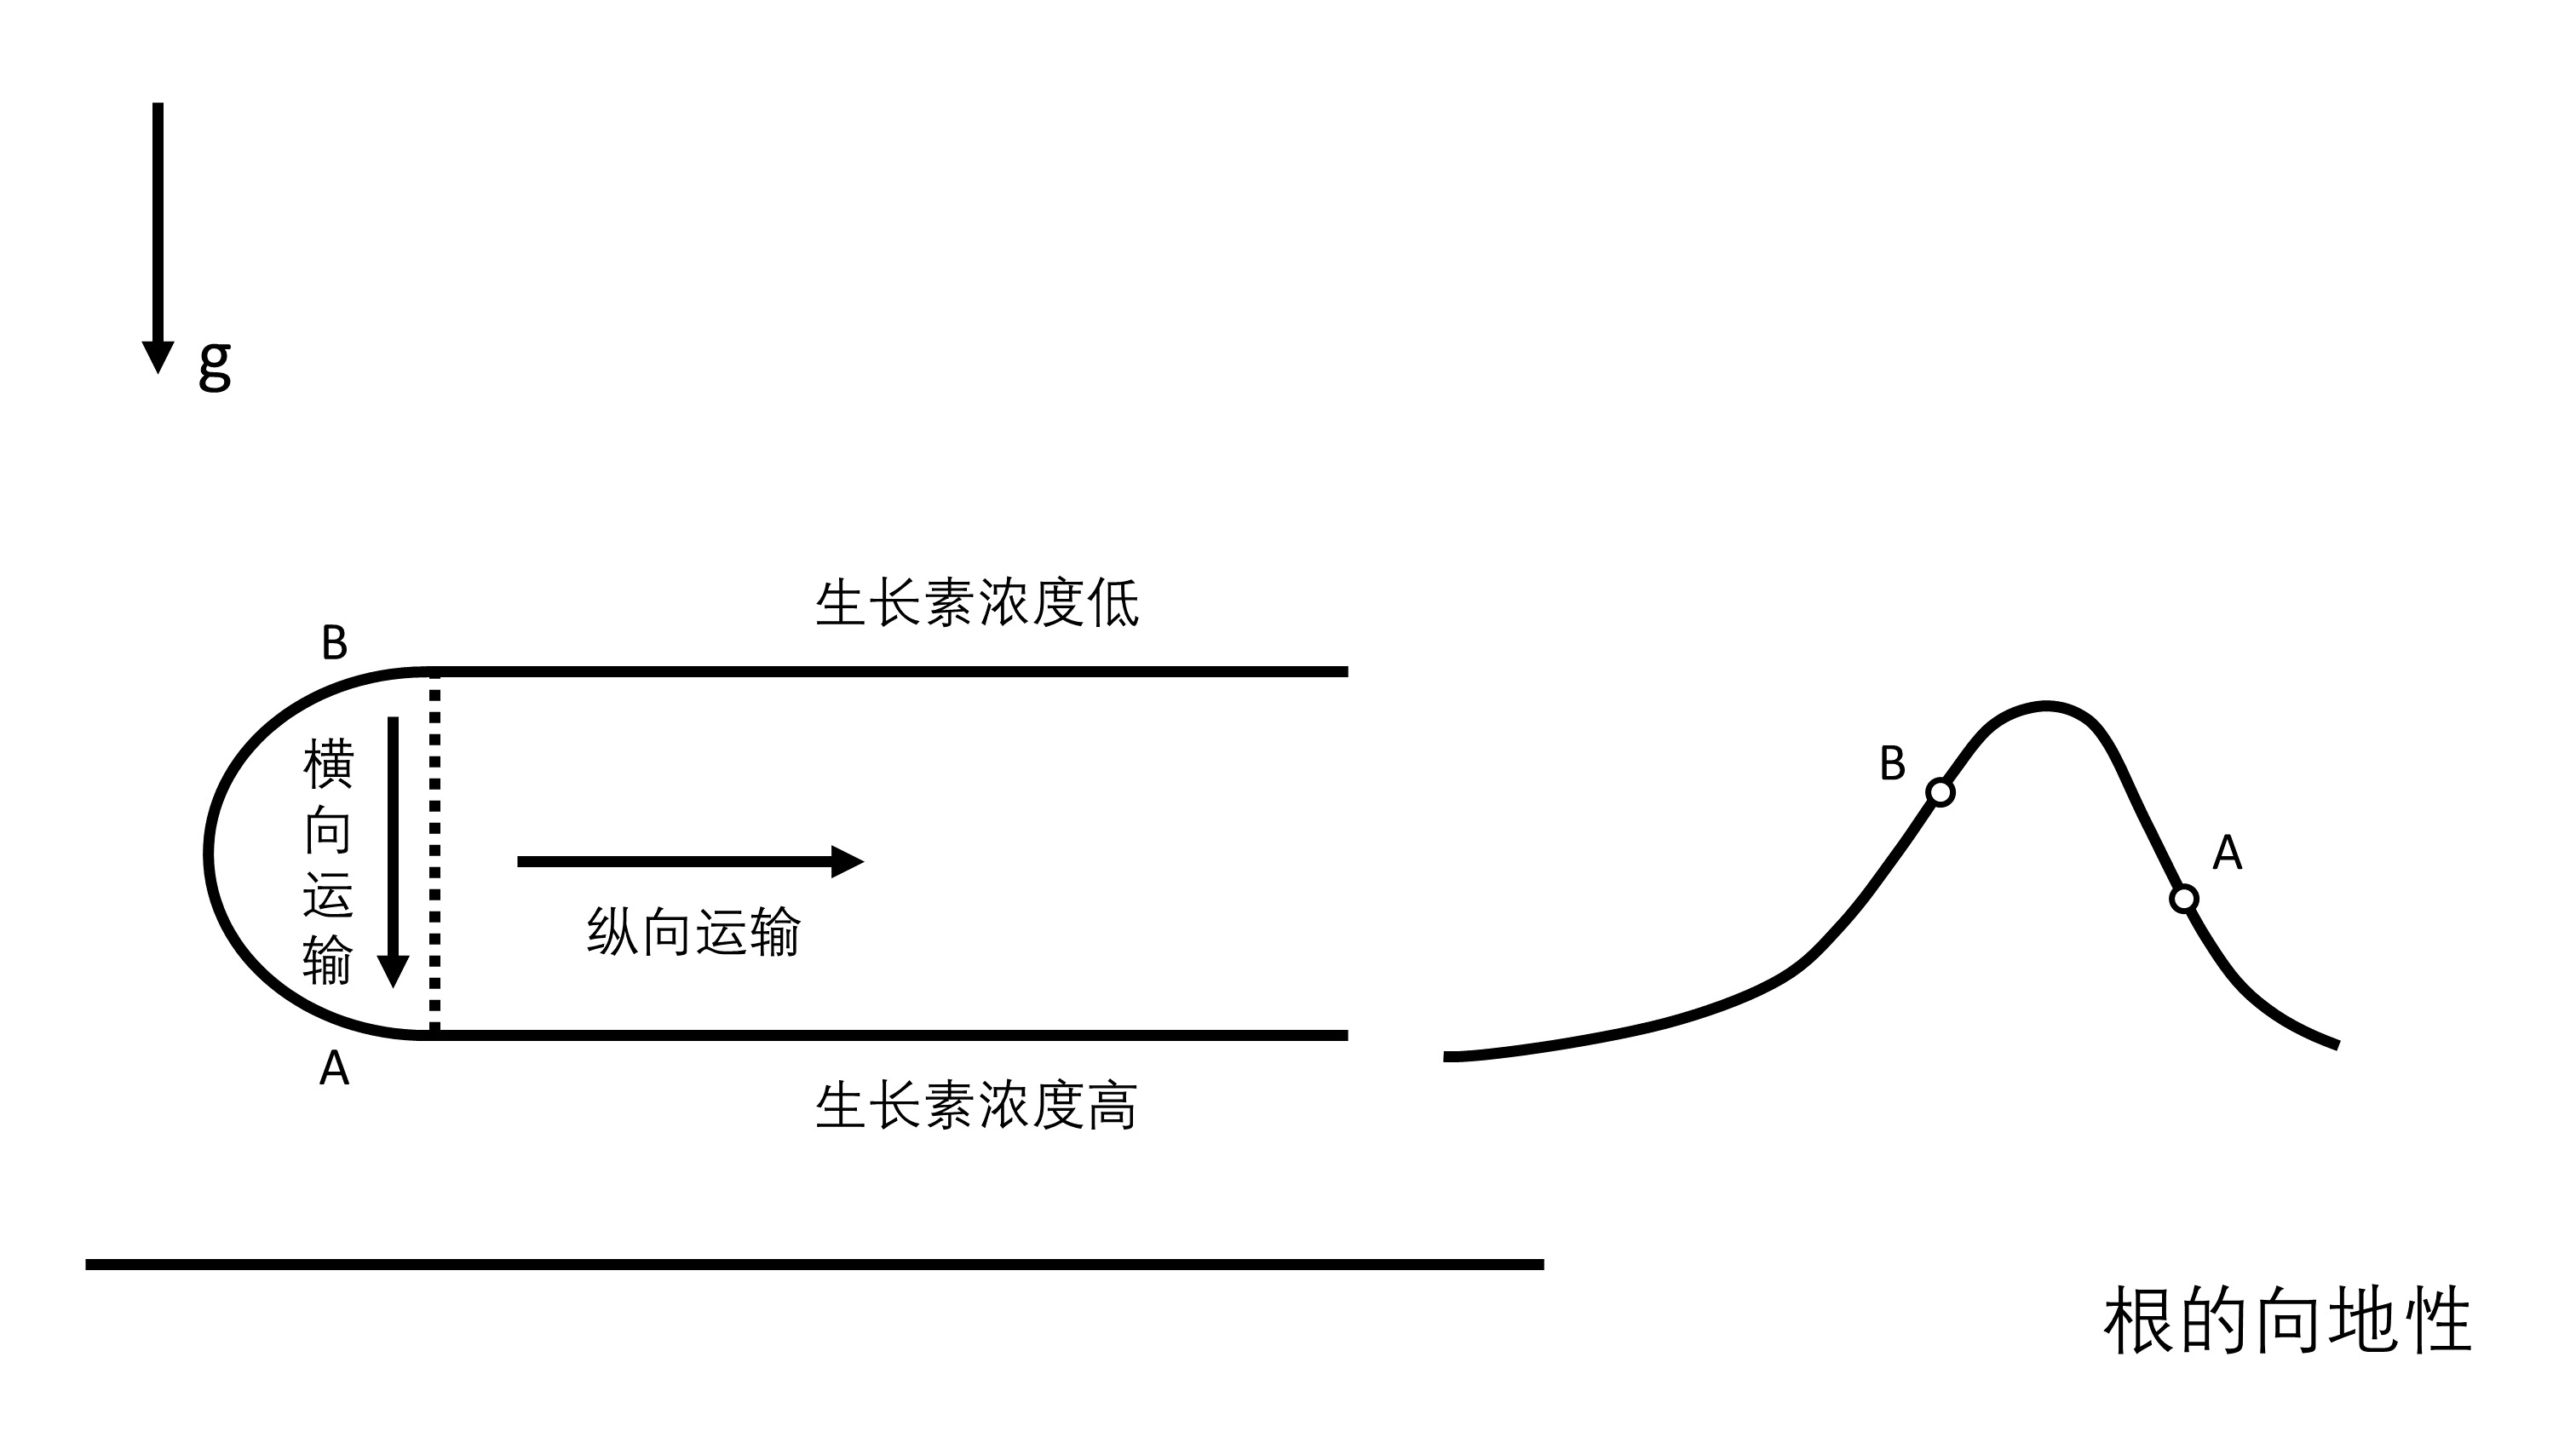
\includegraphics[width=10cm]{BiologyImage/20.jpg}
            \caption{根的向地性}
        \end{center}
    \end{figure}

\newpage

\subsubsection{顶端优势}
    顶芽和侧芽都会分泌生长素,且自身所分泌的生长素均恰好是最适浓度。\\[3mm]
    顶芽所分泌的生长素会纵向运输,越靠近的顶芽的侧芽接收到额外生长素越多,生长越缓慢。\\[3mm]
    因此顶芽可以充分生长,这种现象称为植物的顶端优势,
    顶端优势有助于植物在阴暗的森林中节约养分,
    迅速拔高以突破其他植株叶片的遮盖,从而获得阳光。\\[3mm]
    这就解释了松树杉树等植物的株形为宝塔形的原因。\\[6mm]
    对于果树来说,我们希望其多结果而非多拔高,所以我们可以定期将果树的顶芽切除,
    使侧芽发育为新的顶芽,随后再切除,如此循环。\\[3mm]
    这就解释了苹果树梨树等植物的株形为圆形的原因。\\[6mm]
    下图展示了顶端优势产生的原因:
    \begin{figure}[h!]
        \begin{center}
            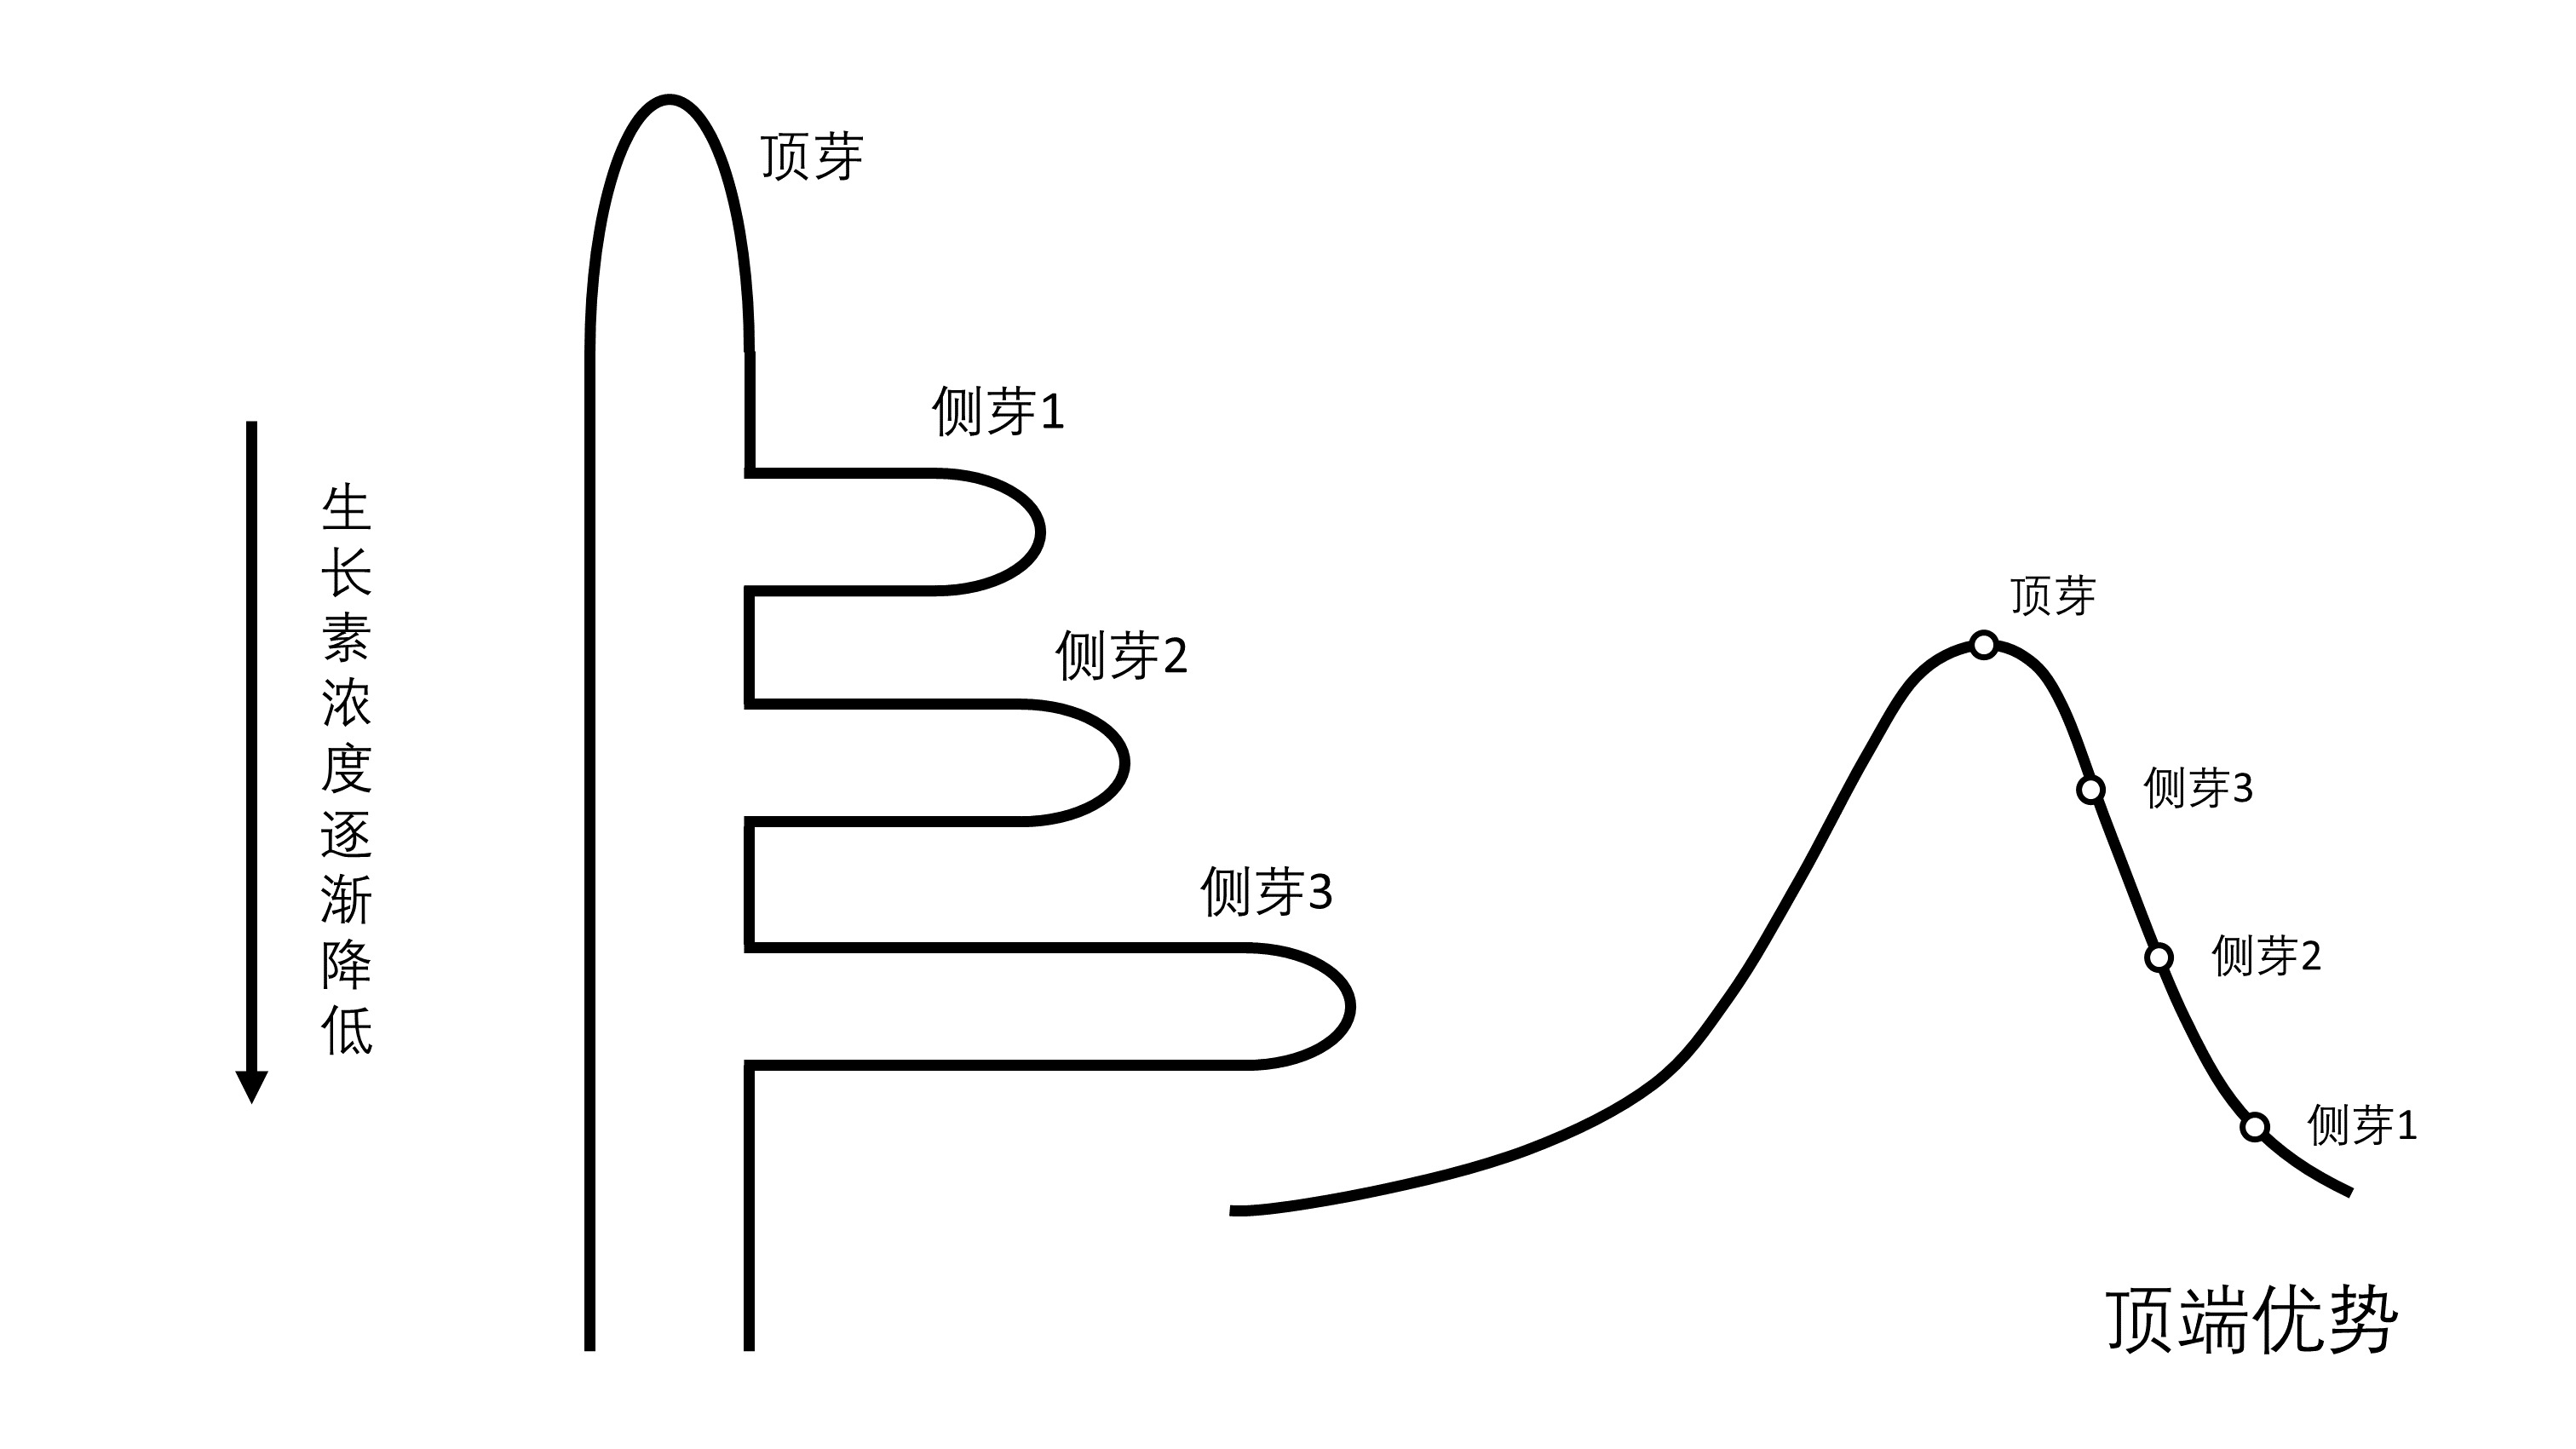
\includegraphics[width=10cm]{BiologyImage/21.jpg}
            \caption{顶端优势}
        \end{center}
    \end{figure}\\
    下图展示了两种株形产生的原因:\vspace{5pt}
    \begin{figure}[h!]
        \begin{center}
            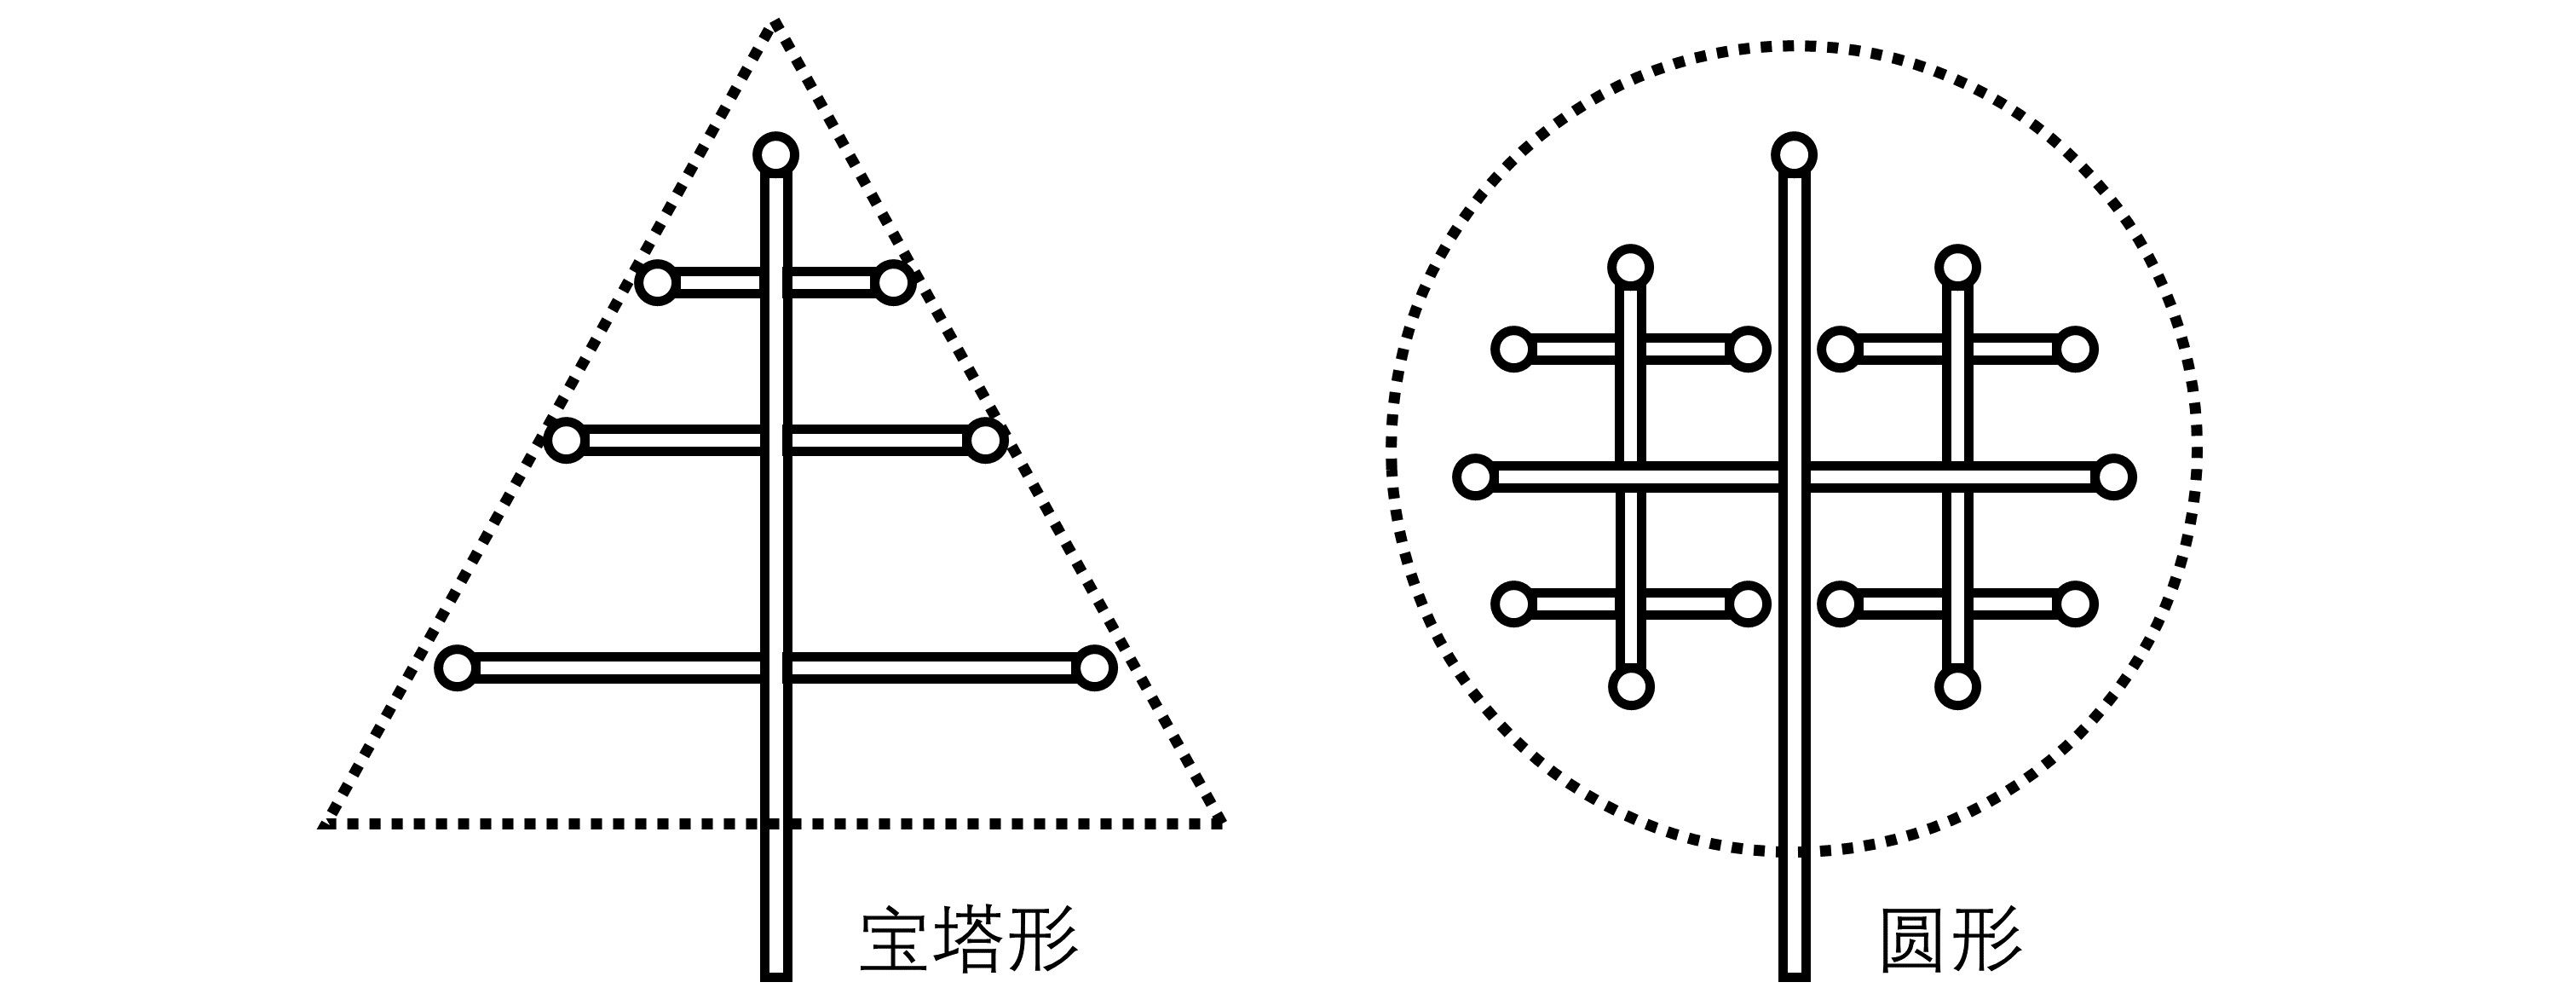
\includegraphics[width=10cm]{BiologyImage/22.jpg}
            \vspace{5pt}
            \caption{两种株形产生的原因}
        \end{center}
    \end{figure}

\newpage

\section{遗传信息的传递和表达}

\subsection{遗传物质}
    现代研究表明,染色体是由脱氧核糖核酸和蛋白质和组成的,其中脱氧核糖核酸是遗传物质。\\[3mm]
    蛋白质是由20种氨基酸组成,脱氧核糖核酸只由4种含氮碱基组成,
    然而脱氧核糖核酸相较于蛋白质仍然更加适合作为遗传物质,
    这是由于遗传物质除了需要存储能力强也需要稳定性强。\\[3mm]
    绝大多数生物的遗传物质是DNA,只有少部分病毒的遗传物质是RNA。

\subsubsection{DNA的分子结构}
    脱氧核苷酸以如下方式连接:\vspace{5pt}
    \begin{figure}[h!]
        \begin{center}
            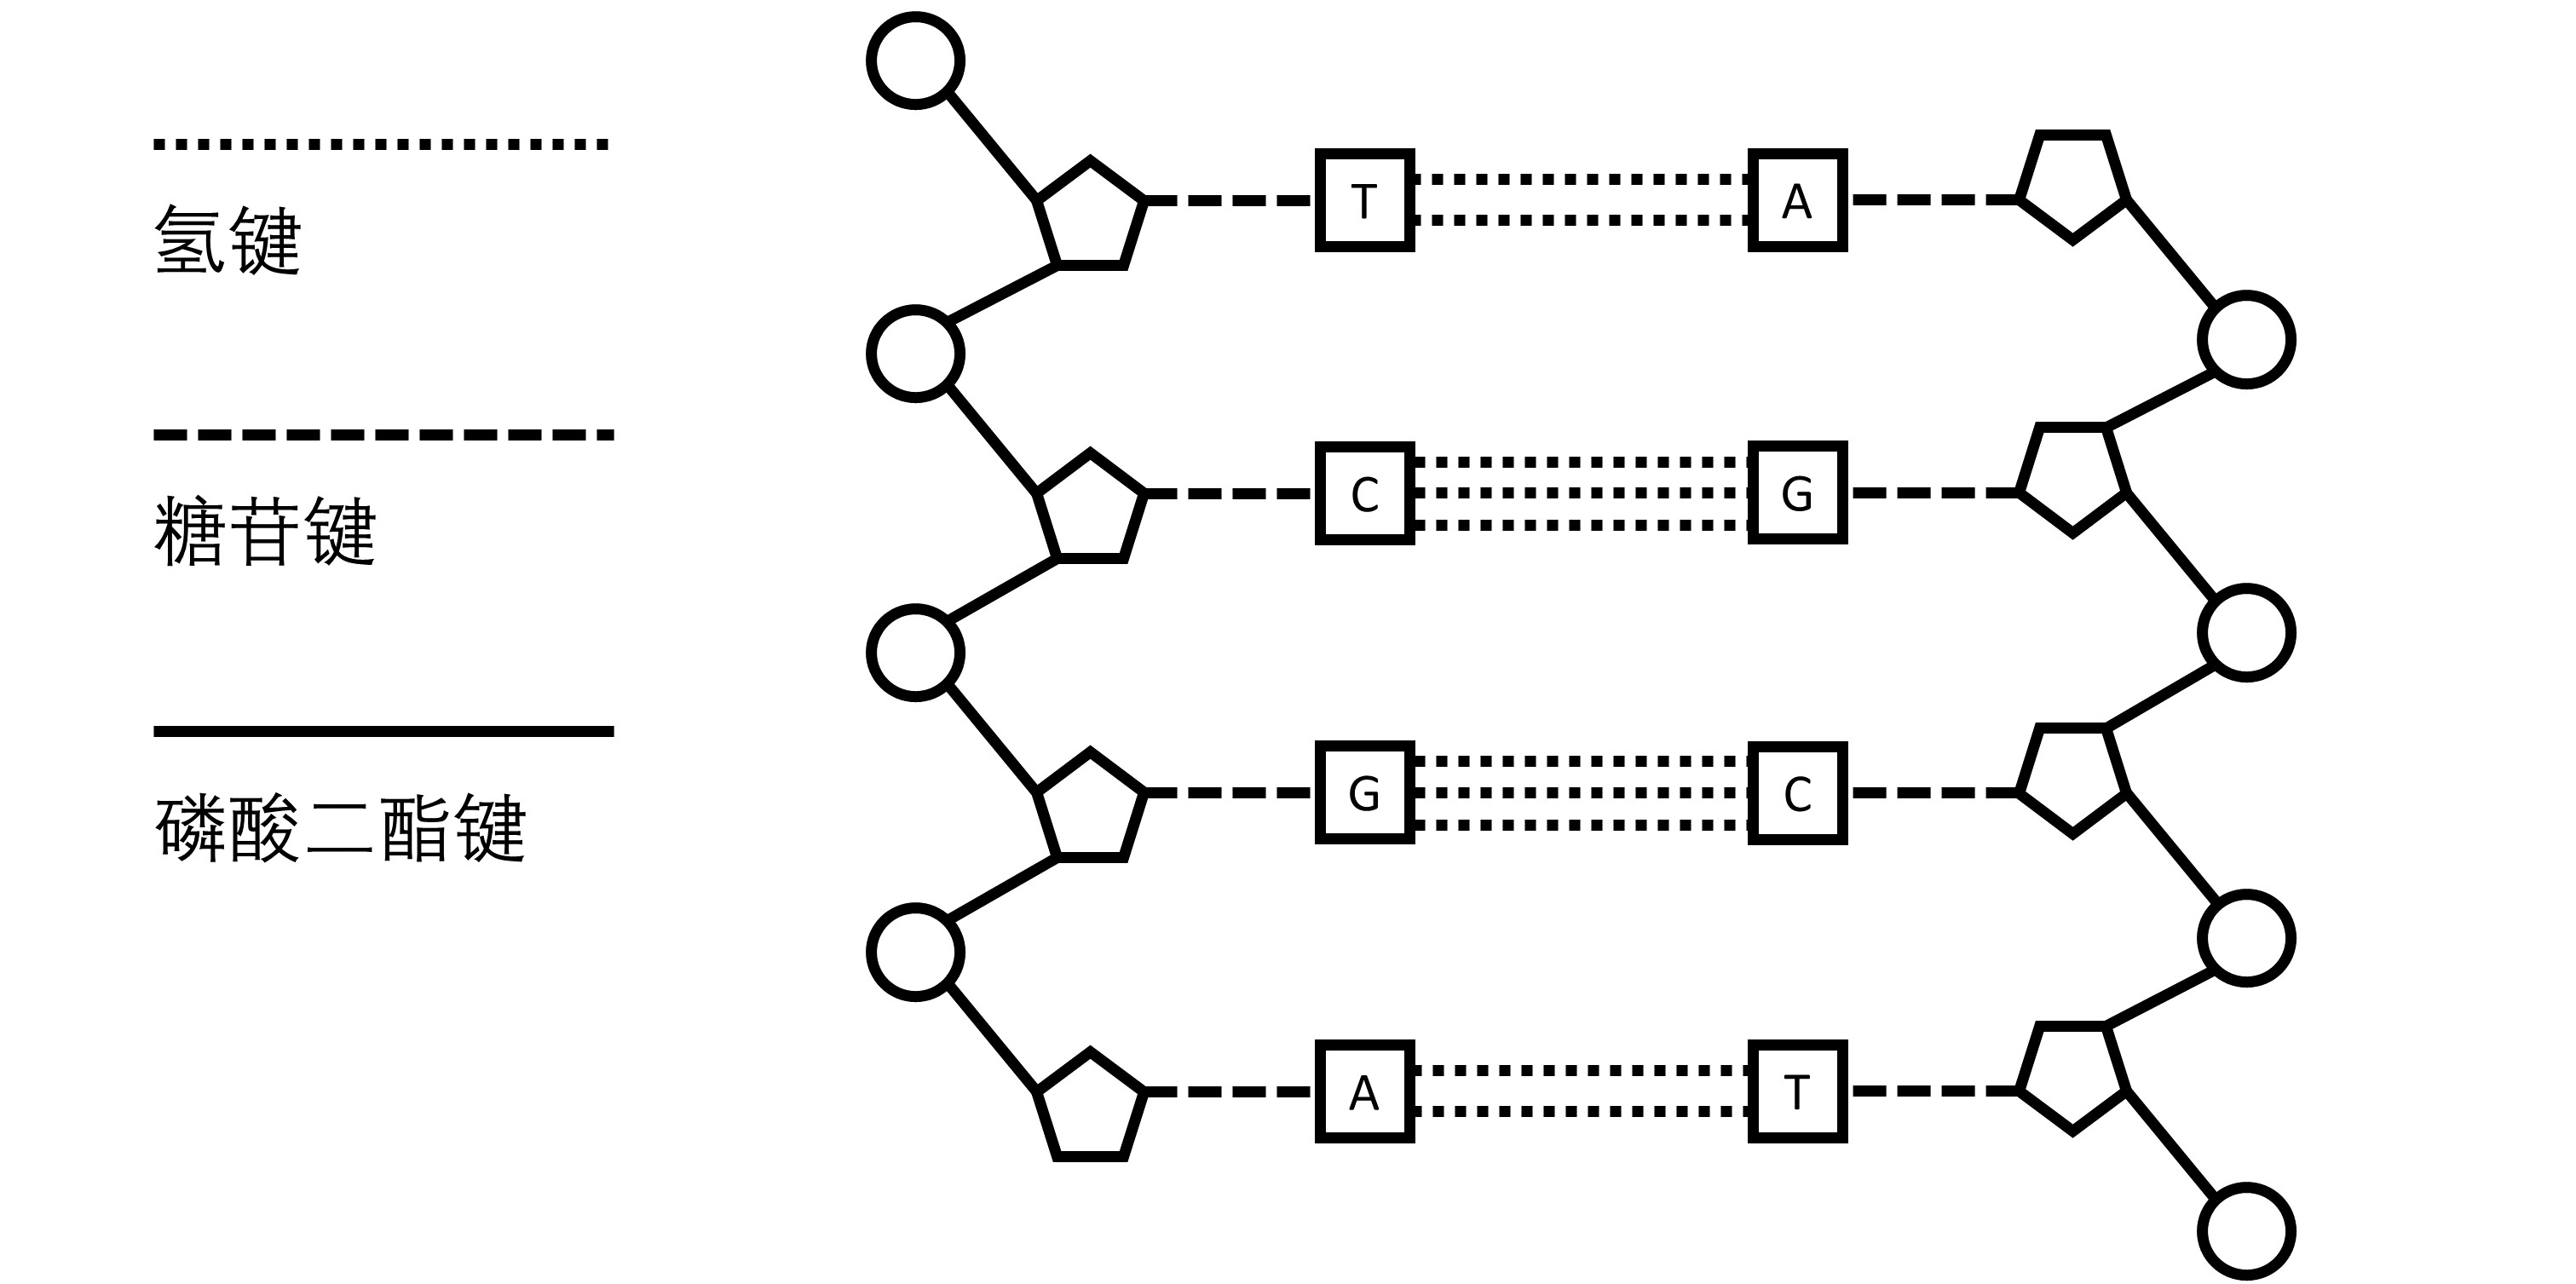
\includegraphics[width=10cm]{BiologyImage/23.jpg}
            \caption{DNA的分子结构}
        \end{center}
    \end{figure}\\
    氢键:连接两个含氮碱基。\\[3mm]
    糖苷键:连接含氮碱基和脱氧核糖。\\[3mm]
    磷酸二酯键:连接磷酸基团和脱氧核糖。\\[6mm]
    含氮碱基间,按照以下规则配对:
    \begin{table}[h!]
        \begin{center}
            \begin{tabular}{l|l|l}
                \hline
                A-T\qquad\qquad&腺嘌呤-胸腺嘧啶\qquad\qquad&两根氢键\qquad\qquad\\ \hline
                G-C\qquad\qquad&鸟嘌呤-胞嘧啶\qquad\qquad&三根氢键\qquad\qquad\\ \hline
            \end{tabular}
            \caption{含氮碱基的配对规则}
        \end{center}
    \end{table}

\subsubsection{DNA的双螺旋结构}
    脱氧核糖核酸分子实际上是呈双螺旋结构,脱氧核苷酸通过上方的方式连接后,在空间层面上,
    每一对碱基在上一对碱基的基础上需要旋转$36$度,也就是每十对碱基旋转$360$度。

\newpage

\subsection{DNA的复制}
    DNA的复制:以DNA为模板合成DNA的过程。\\[3mm]
    1.组成DNA分子的两条链在DNA解旋酶的作用下逐渐分开。\\[3mm]
    2.以DNA分子的两条链为模板,依照碱基配对规则,与细胞中游离的脱氧核苷酸配对。\\[3mm]
    3.组成DNA子链的脱氧核苷酸在DNA聚合酶的作用下互相连接。\\[6mm]
    由此可见,DNA复制是一个边解旋边复制,DNA的复制形式也被称为半保留复制。

\subsection{DNA的转录}
    DNA的转录:以DNA为模板合成RNA的过程。\\[3mm]
    1.组成DNA分子的两条链在DNA解旋酶的作用下逐渐分开。\\[3mm]
    2.以DNA分子的一条链为模板,依照碱基配对规则,与细胞中游离的核糖核苷酸配对。\\[3mm]
    3.组成RNA链的核糖核苷酸在RNA聚合酶的作用下互相连接。\\[6mm]
    转录过程的重要意义在于,DNA的体积较大,无法穿过核孔,RNA的体积较小,可以穿过核孔,
    通过RNA可以将DNA上的遗传信息通过核孔带出细胞核,从而实现遗传信息的传递。

\subsection{RNA的翻译}
    RNA的翻译:以mRNA为模板,以tRNA为工具,合成蛋白质的过程。\\[3mm]
    1.转录所产生的mRNA进入核糖体。\\[3mm]
    2.携带氨基酸的tRNA进入核糖体。\\[3mm]
    3.以mRNA上三个碱基组成的密码子,与tRNA上三个碱基组成的反密码子,两者配对。\\[3mm]
    4.上一个进入核糖体的tRNA所携带的肽链连接到当前tRNA,随后离开核糖体。\\[3mm]
    5.此后循环第二步至第四步,直到出现没有对应tRNA的终止密码子时,翻译终止。\\[6mm]
    下表列出了各个类型RNA的定义:
    \begin{table}[h]
        \begin{center}
            \begin{tabular}{l|l|l}
                \hline
                mRNA\qquad\qquad&信使RNA\qquad\qquad&转录过程的产物\qquad\qquad\\ \hline
                tRNA\qquad\qquad&转运RNA\qquad\qquad&翻译过程的工具\qquad\qquad\\ \hline
                rRNA\qquad\qquad&核糖体RNA\qquad\qquad&核糖体的组成部分,用途不明\qquad\qquad\\ \hline
            \end{tabular}
            \caption{RNA的类型}
        \end{center}
    \end{table}

\newpage

\subsection{遗传物质相关酶}
    以下表格列出了与遗传物质相关的酶:
    \begin{table}[h]
        \begin{center}
            \begin{tabular}{l|l|l|l}
                \hline
                DNA解旋酶\qquad\qquad&DNA复制&断开氢键\qquad\qquad&使得双链DNA解旋为两条单链\qquad\qquad\\ \hline
                DNA聚合酶\qquad\qquad&DNA复制&连接磷酸二酯键\qquad\qquad&将脱氧核苷酸聚合为DNA单链\\ \hline
                RNA聚合酶\qquad\qquad&DNA转录&连接磷酸二酯键\qquad\qquad&将脱氧核苷酸聚合为RNA单链\\ \hline
                DNA连接酶\qquad\qquad&基因工程&连接磷酸二酯键\qquad\qquad&切割黏性末端\\ \hline
                限制性核酸内切酶\qquad\qquad&基因工程&断开磷酸二酯键\qquad\qquad&连接黏性末端\\ \hline
            \end{tabular}
            \caption{遗传物质相关酶的作用}
        \end{center}
    \end{table}\\
    需要指出的是,当磷酸二酯键在酶的作用下连接或断开时,对应位置的氢键会自行连接或断开,
    这是由于氢键的作用力非常弱,因此可以在不需要酶作用的情况下自行连接或断开。\\[3mm]
    需要说明的是,虽然在转录中我们提到转录过程需要DNA解旋酶的参与,但是实际上转录过程的解旋是一个非常复杂的过程,
    并不是单纯依靠DNA解旋酶完成的,因此上方表格中在DNA解旋酶一栏中没有提到其可以用转录过程。

\newpage

\section{细胞的分裂和分化}

\subsection{生殖方式}
    物种得以延续的前提是个体具有生殖能力,并在个体死亡前通过生殖留下后代。

\subsubsection{无性生殖}
    无性生殖:不经过生殖细胞的结合,由母体直接产生新个体的生殖方式。\\[3mm]
    无性生殖的四种常见方式:分裂生殖,出芽生殖,孢子生殖,营养繁殖。\\[3mm]
    分裂生殖:草履虫,眼虫,硅藻。\\[2mm]
    出芽生殖:酵母菌,水螅。\\[2mm]
    孢子生殖:真菌,苔藓,蕨类。\\[2mm]
    营养繁殖:马铃薯的块茎,甘薯的块根,落地生根的叶,草莓的匍匐茎,香蕉的地下茎。\\[5mm]
    无性生殖的繁殖速度较快,但由于个体基因来自于同一亲本,所以不利于遗传信息的组合。\\[3mm]
    无性生殖的生物因此对环境变化的适应能力较弱。

\subsubsection{有性生殖}
    有性生殖:通过亲本产生的雌雄生殖细胞结合形成受精卵,发育为新个体的生殖方式。\\[3mm]
    雄性生殖细胞称为精子,体积小,数量多,活动能力较强。\\[3mm]
    雌性生殖细胞称为卵子,体积大,数量少,活动能力丧失。\\[5mm]
    精子和卵子结合为受精卵的过程,称为受精作用。\\[3mm]
    受精时,有许多精子同时游向卵子,但只有一个精子能与卵子完成受精作用。\\[3mm]
    受精时,精子的头部穿过卵膜,精子的尾部仍留在卵膜外,精子的细胞核与卵子的细胞核融合。\\[5mm]
    有性生殖的繁殖速度较慢,但由于个体基因来自于不同亲本,所以有利于遗传信息的组合。\\[3mm]
    有性生殖的生物因此对环境变化的适应能力较强。

\subsection{有丝分裂}
    有丝分裂是动植物细胞分裂的主要方式。\\[3mm]
    经过有丝分裂,分裂期间复制的DNA平均分离,产生两个染色体数目与形态结构与亲代细胞完全相同的子细胞,
    保证亲代和子代之间遗传性状的稳定性和连续性。

\newpage

\subsubsection{有丝分裂间期}
    有丝分裂间期:细胞核内染色质呈细丝状,细胞核内的核仁十分明显,间期完成了DNA的复制。\\[3mm]
    有丝分裂间期分为三个阶段:DNA合成前期,DNA合成期,DNA合成后期。\vspace{5pt}
    \begin{table}[h]
        \begin{center}
            \begin{tabular}{l|l|l}
                \hline
                DNA合成前期\qquad\qquad&G$_1$期\qquad\qquad&合成蛋白质,主要是与复制有关的酶\qquad\qquad\\ \hline
                DNA合成期\qquad\qquad&S期\qquad\qquad&进行DNA的精确复制\qquad\qquad\\ \hline
                DNA合成后期\qquad\qquad&G$_2$期\qquad\qquad&合成蛋白质,主要是与组装纺锤体有关\qquad\qquad\\ \hline
            \end{tabular}
            \caption{间期的三个阶段}
        \end{center}
    \end{table}\\
    对于植物细胞,其没有中心体,对于动物细胞,其中心体会在该阶段复制。\\[6mm]
    植物的有丝分裂间期:
    \begin{figure}[h]
        \begin{center}
            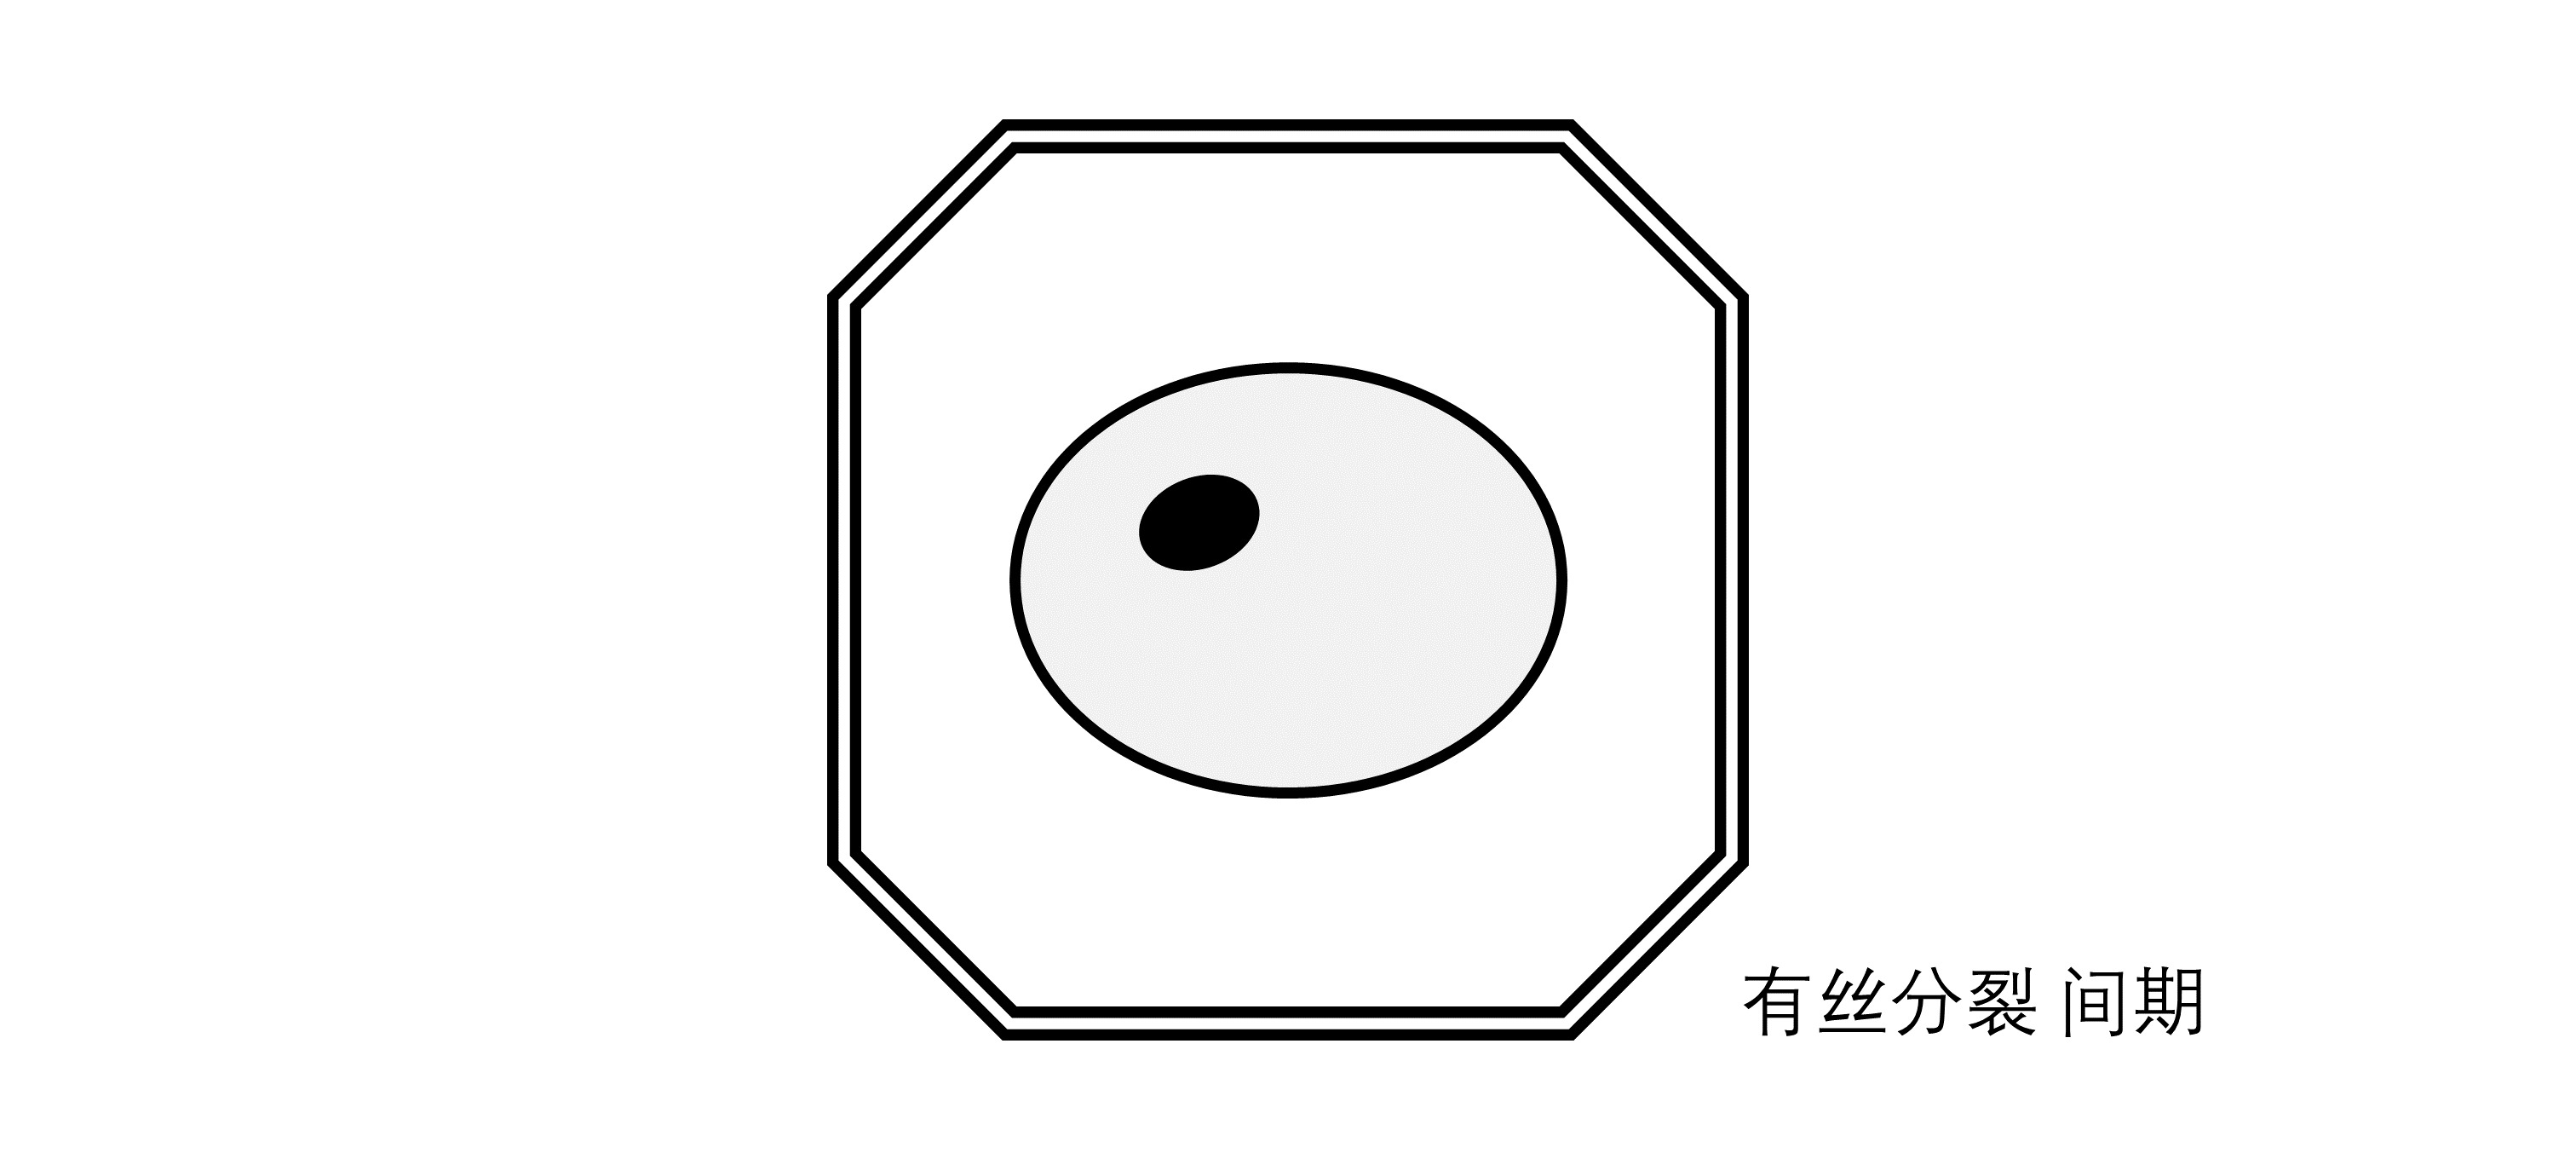
\includegraphics[width=10cm]{BiologyImage/24.jpg}
            \caption{植物的有丝分裂间期}
        \end{center}
    \end{figure}\\
    动物的有丝分裂间期:
    \begin{figure}[h]
        \begin{center}
            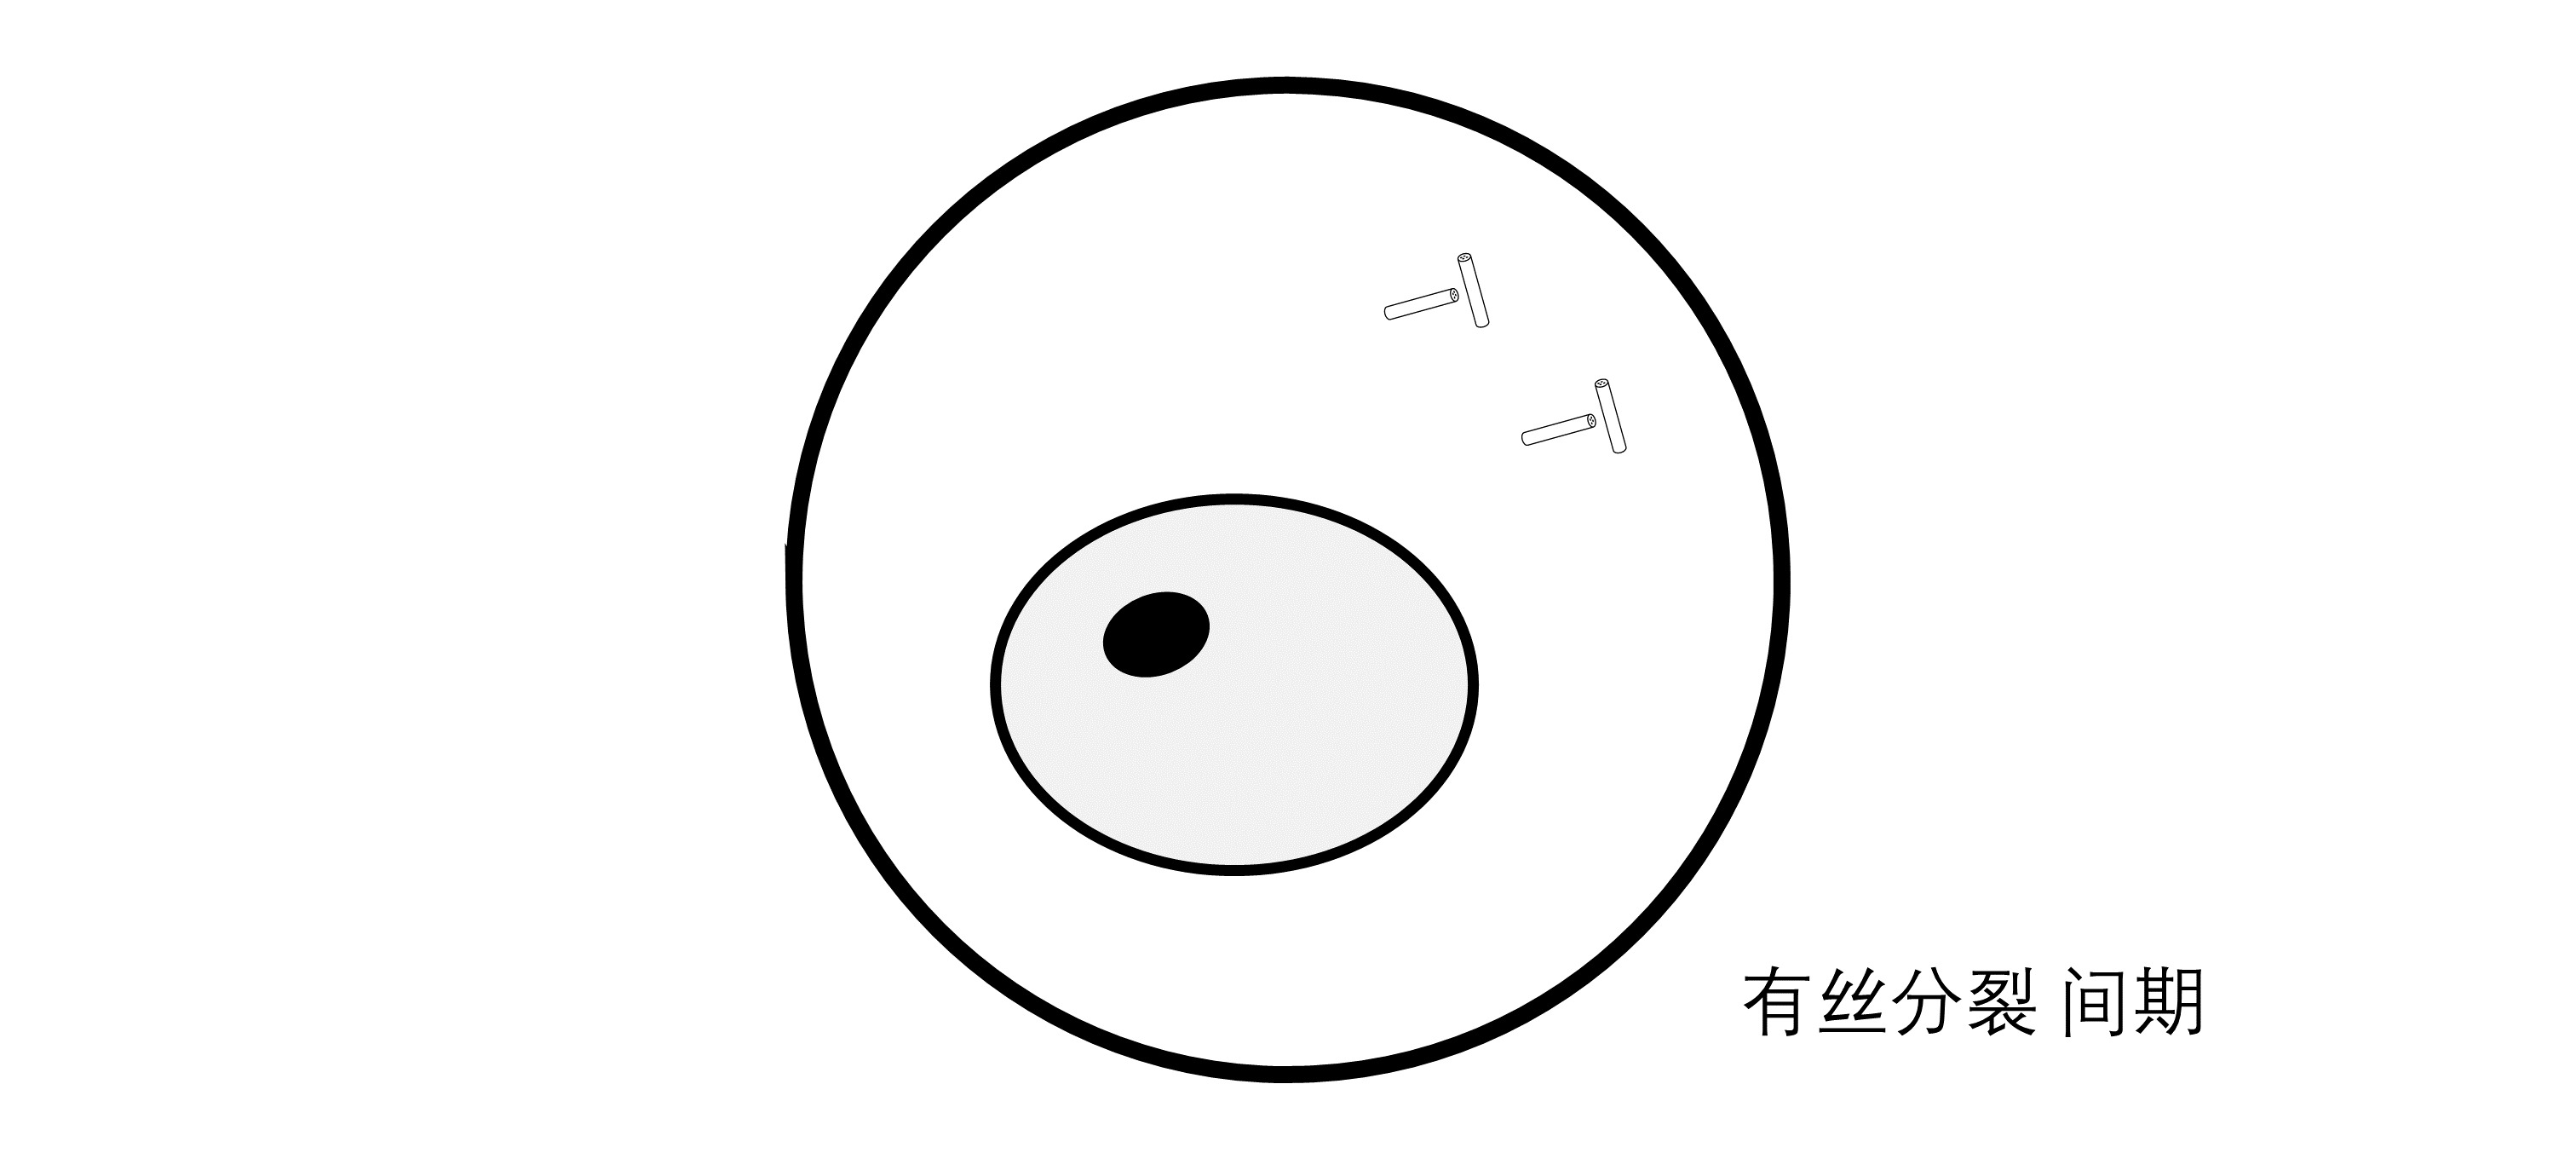
\includegraphics[width=10cm]{BiologyImage/29.jpg}
            \caption{动物的有丝分裂间期}
        \end{center}
    \end{figure}\\

\subsubsection{有丝分裂前期}
    有丝分裂前期:核仁和核膜消失,染色质螺旋缠绕形成染色体,细胞中出现了梭形的纺锤体。\\[3mm]
    对于植物细胞,纺锤体的纺锤丝由两极发出,对于动物细胞,纺锤体的纺锤丝由中心体发出。\\[6mm]
    植物的有丝分裂前期:
    \begin{figure}[h]
        \begin{center}
            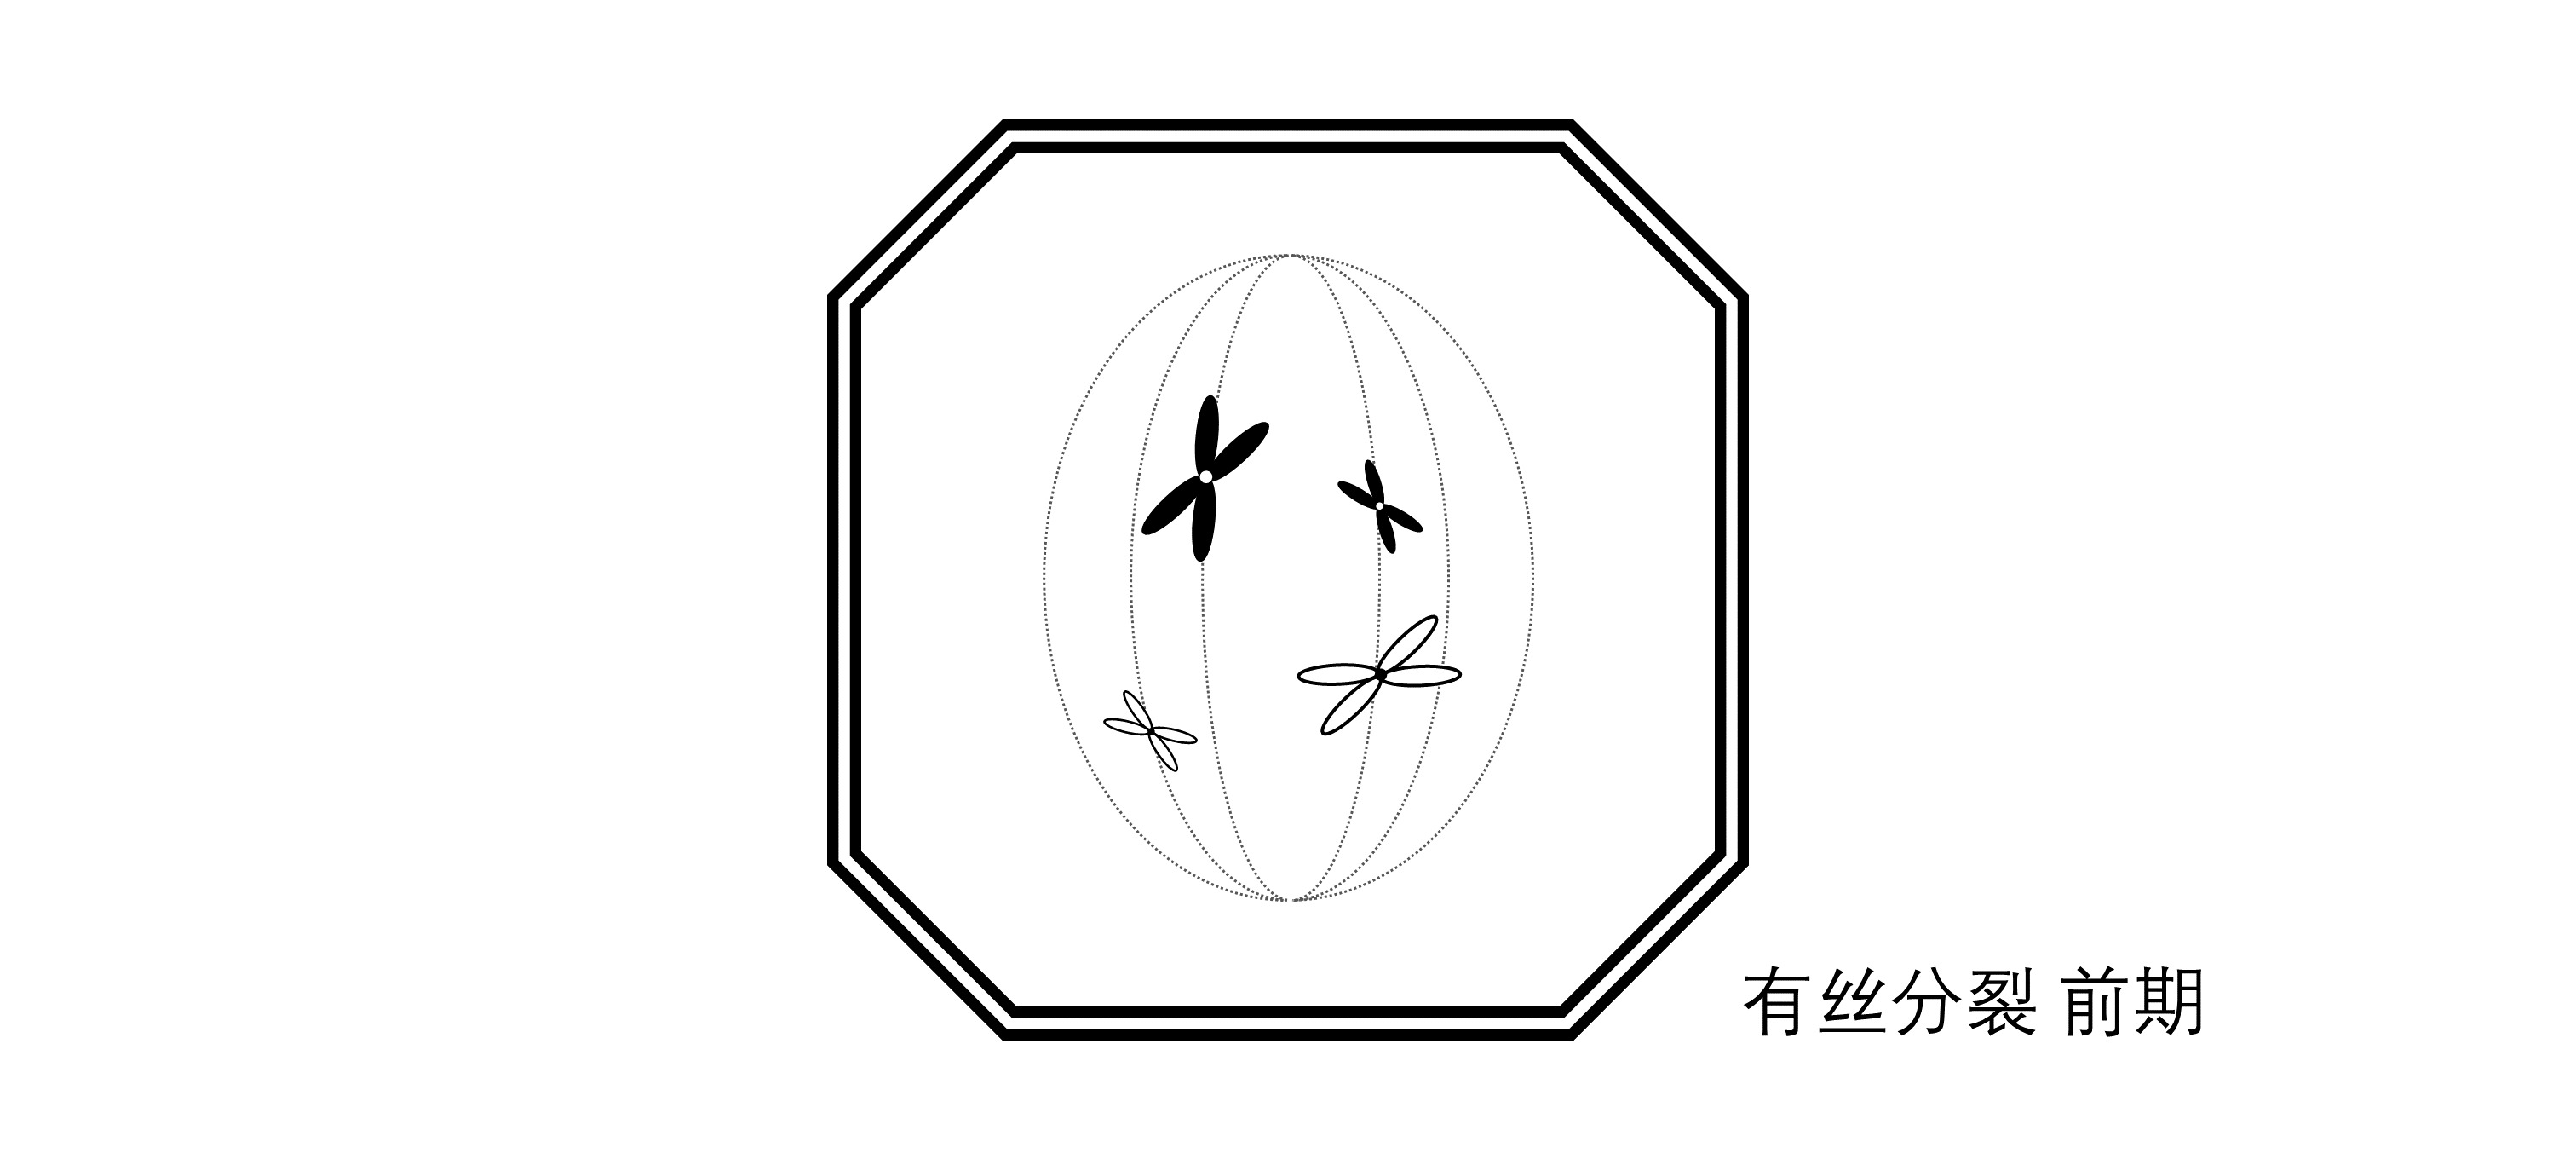
\includegraphics[width=10cm]{BiologyImage/25.jpg}
            \caption{植物的有丝分裂前期}
        \end{center}
    \end{figure}\\
    动物的有丝分裂前期:
    \begin{figure}[h]
        \begin{center}
            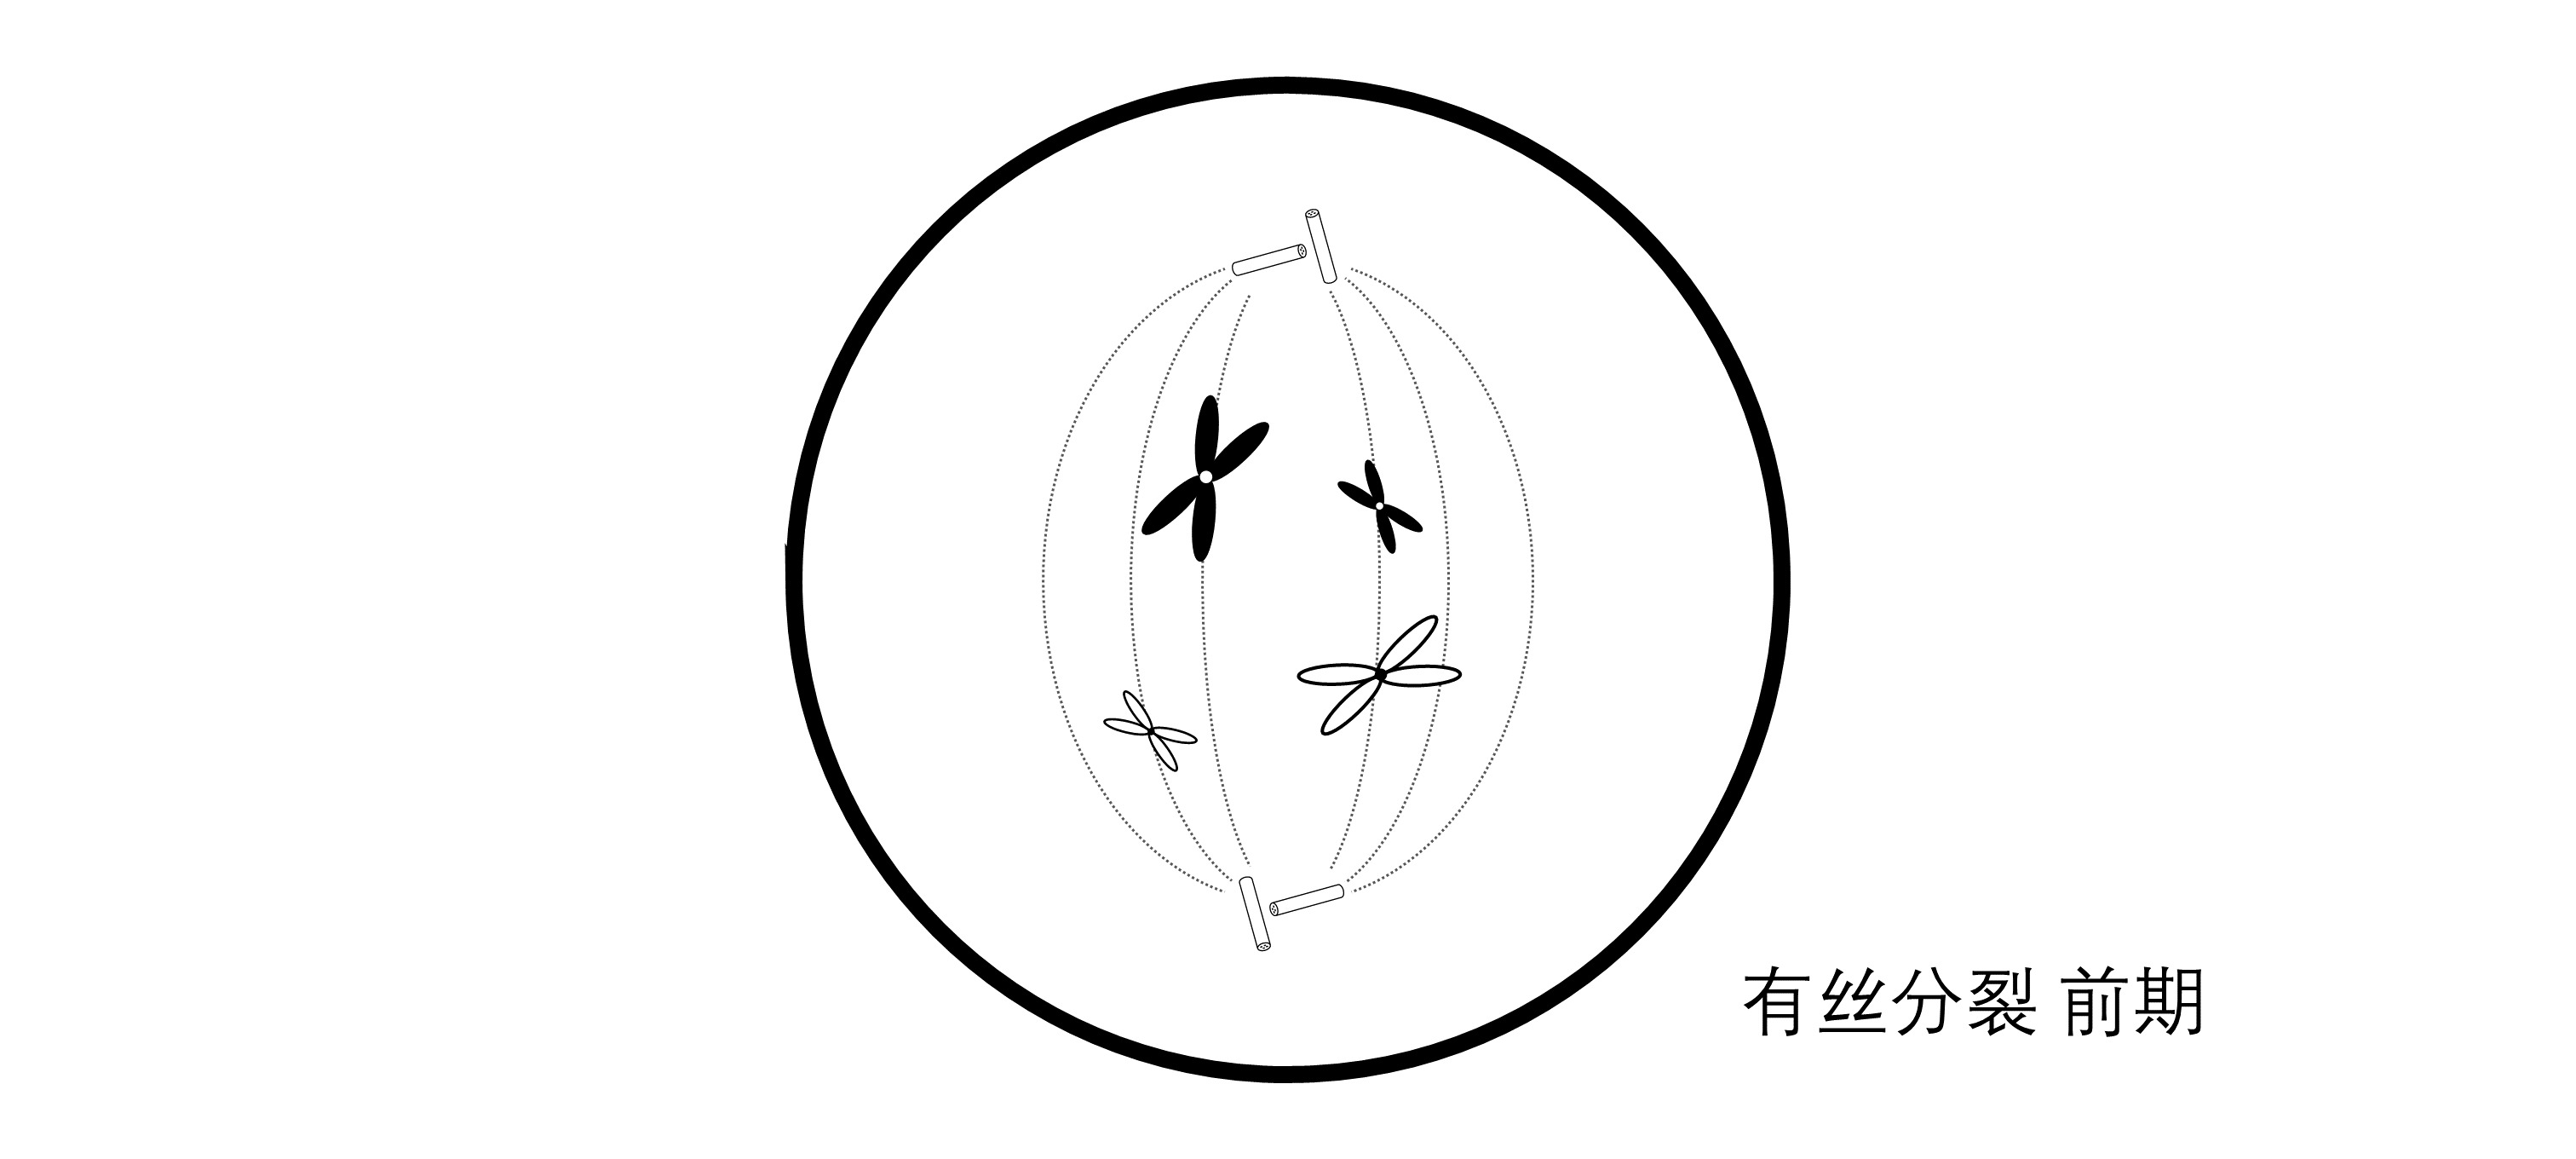
\includegraphics[width=10cm]{BiologyImage/30.jpg}
            \caption{动物的有丝分裂前期}
        \end{center}
    \end{figure}\\

\newpage

\subsubsection{有丝分裂中期}
    有丝分裂中期:着丝粒与纺锤丝相连,染色体在纺锤丝的牵引下排列赤道面。\\[3mm]
    对于植物细胞,纺锤体的纺锤丝由两极发出,对于动物细胞,纺锤体的纺锤丝由中心体发出。\\[6mm]
    植物的有丝分裂中期:
    \begin{figure}[h]
        \begin{center}
            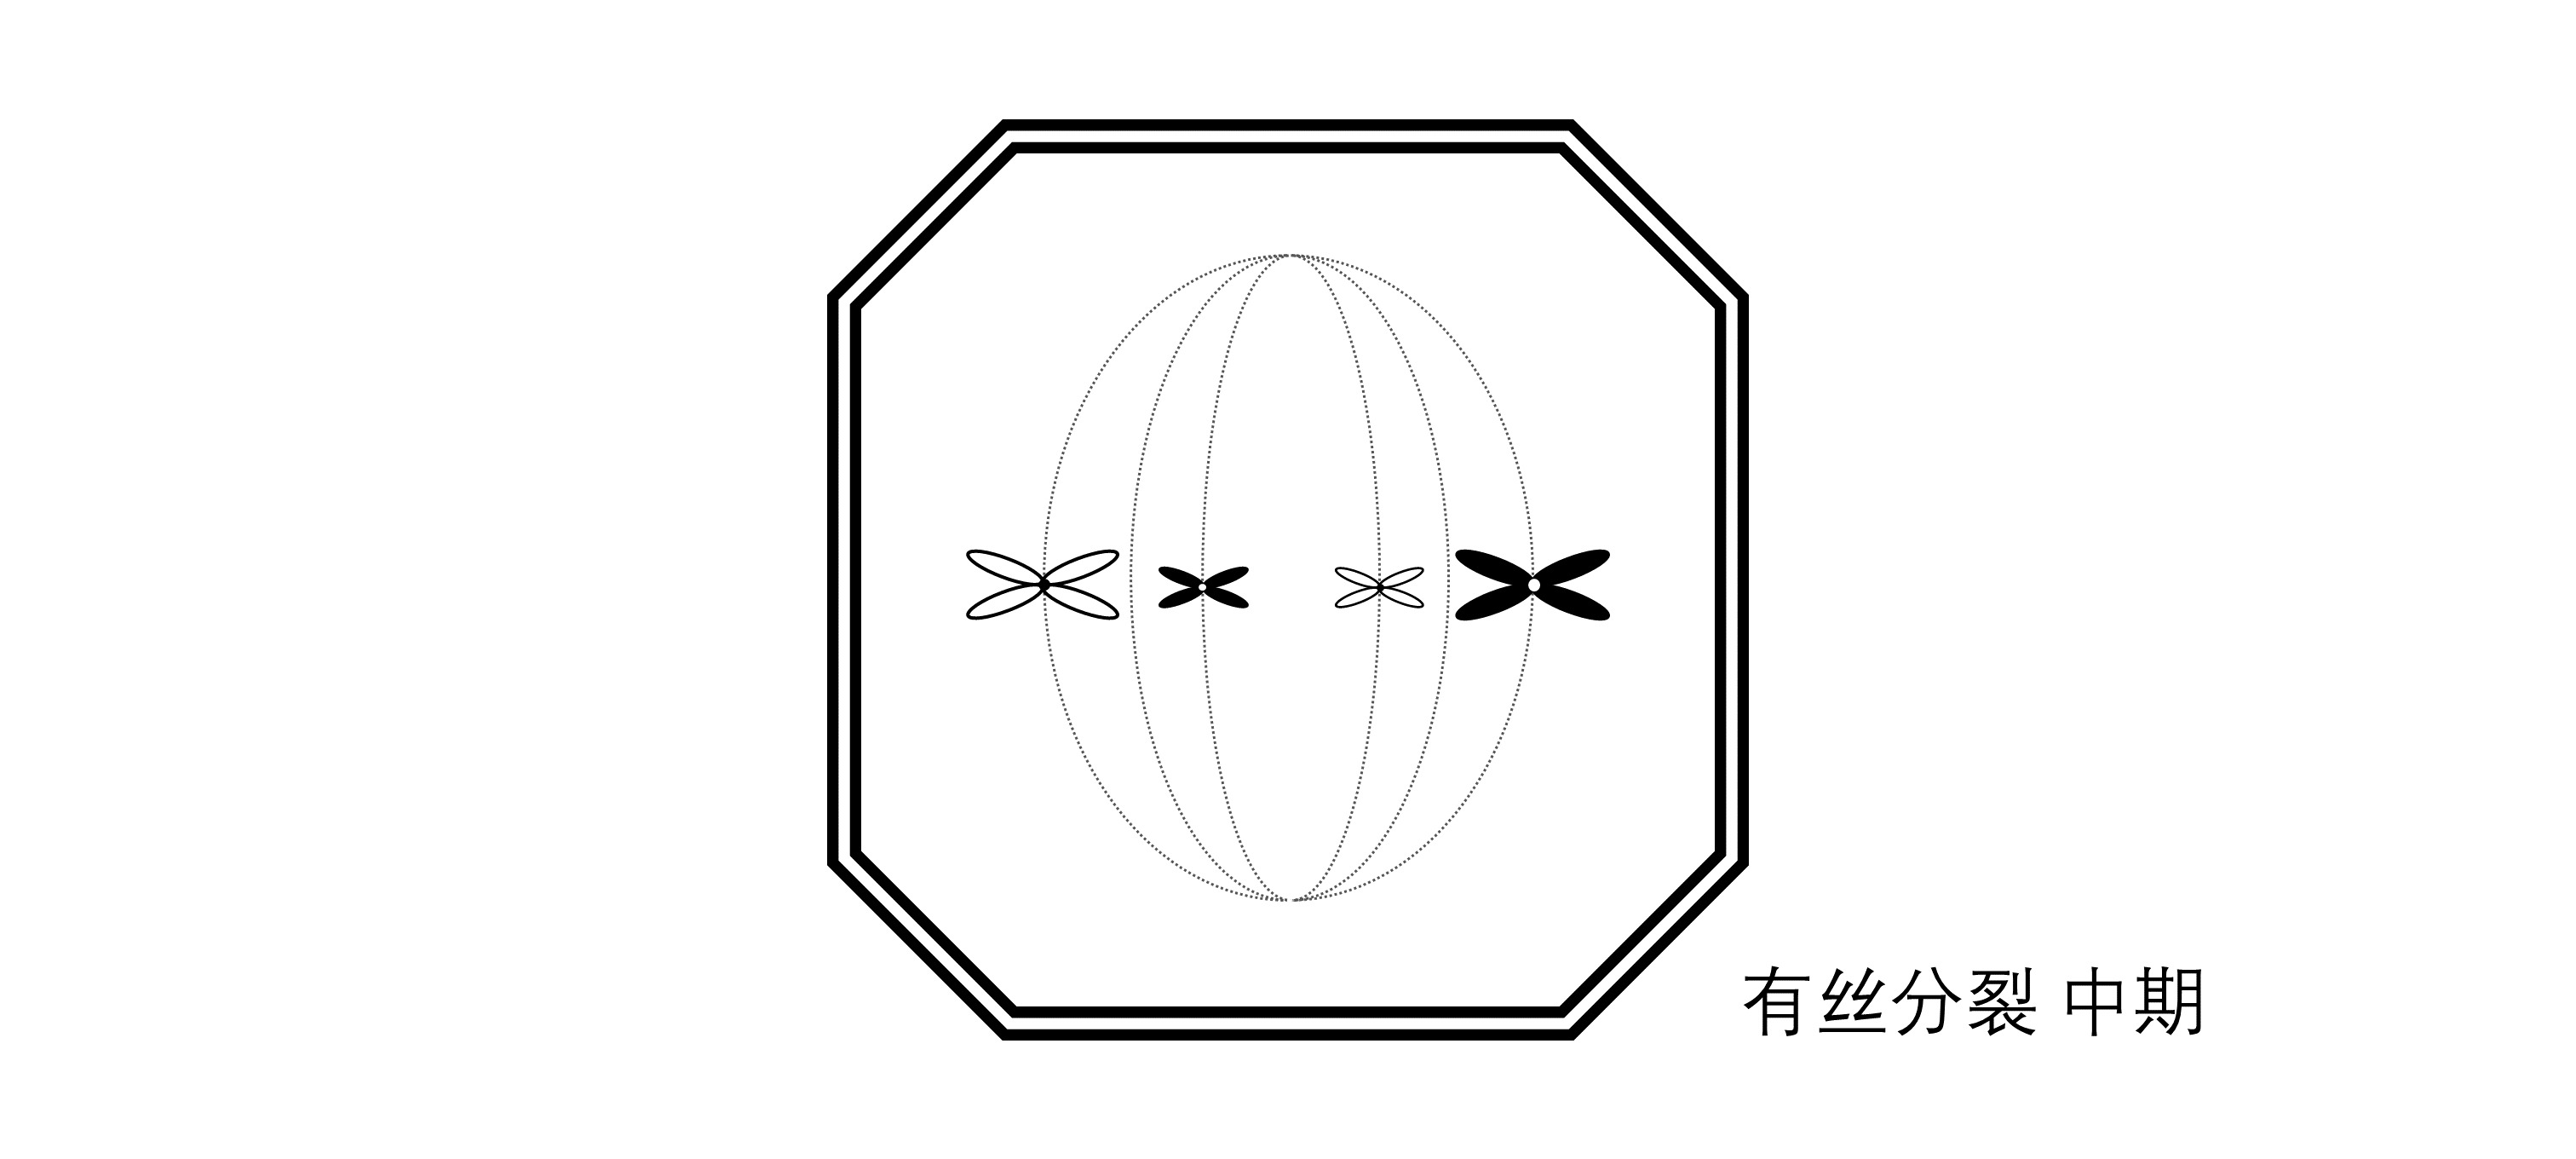
\includegraphics[width=10cm]{BiologyImage/26.jpg}
            \caption{植物的有丝分裂中期}
        \end{center}
    \end{figure}\\
    动物的有丝分裂中期:
    \begin{figure}[h]
        \begin{center}
            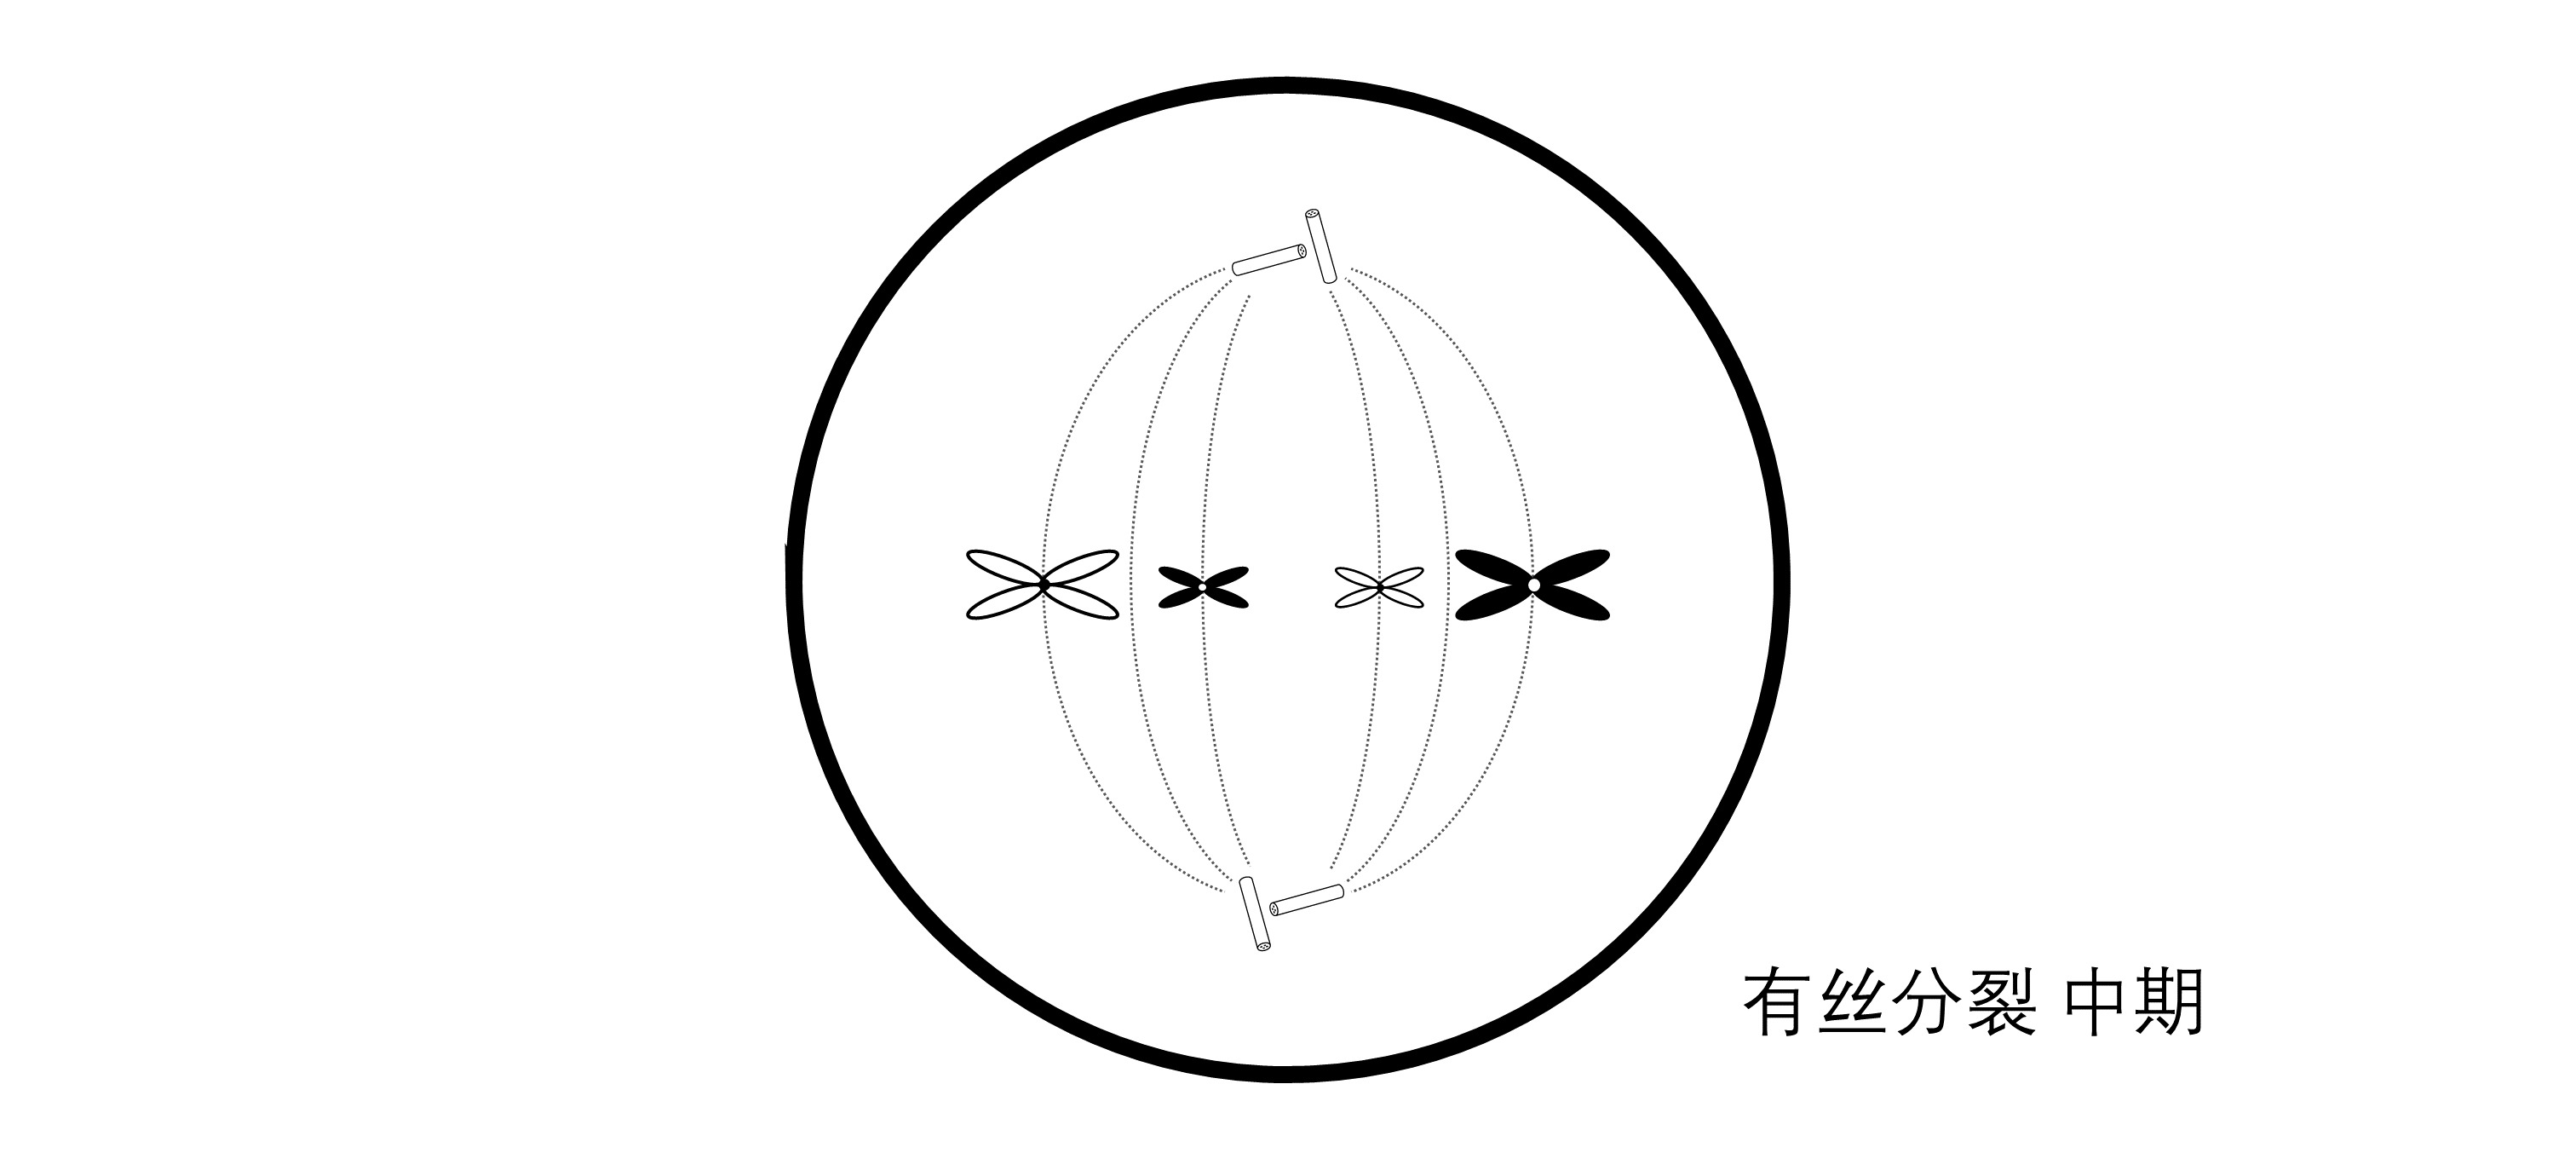
\includegraphics[width=10cm]{BiologyImage/31.jpg}
            \caption{动物的有丝分裂中期}
        \end{center}
    \end{figure}\\

\newpage

\subsubsection{有丝分裂后期}
    有丝分裂后期:着丝粒分裂为两个,染色体中两条染色单体分开,成为两条完全独立的染色体,
    在纺锤丝的牵引下分别移向两极,形成两组形态结构数目与亲代细胞完全相同的染色体。\\[3mm]
    对于植物细胞,纺锤体的纺锤丝由两极发出,对于动物细胞,纺锤体的纺锤丝由中心体发出。\\[6mm]
    植物的有丝分裂后期:
    \begin{figure}[h]
        \begin{center}
            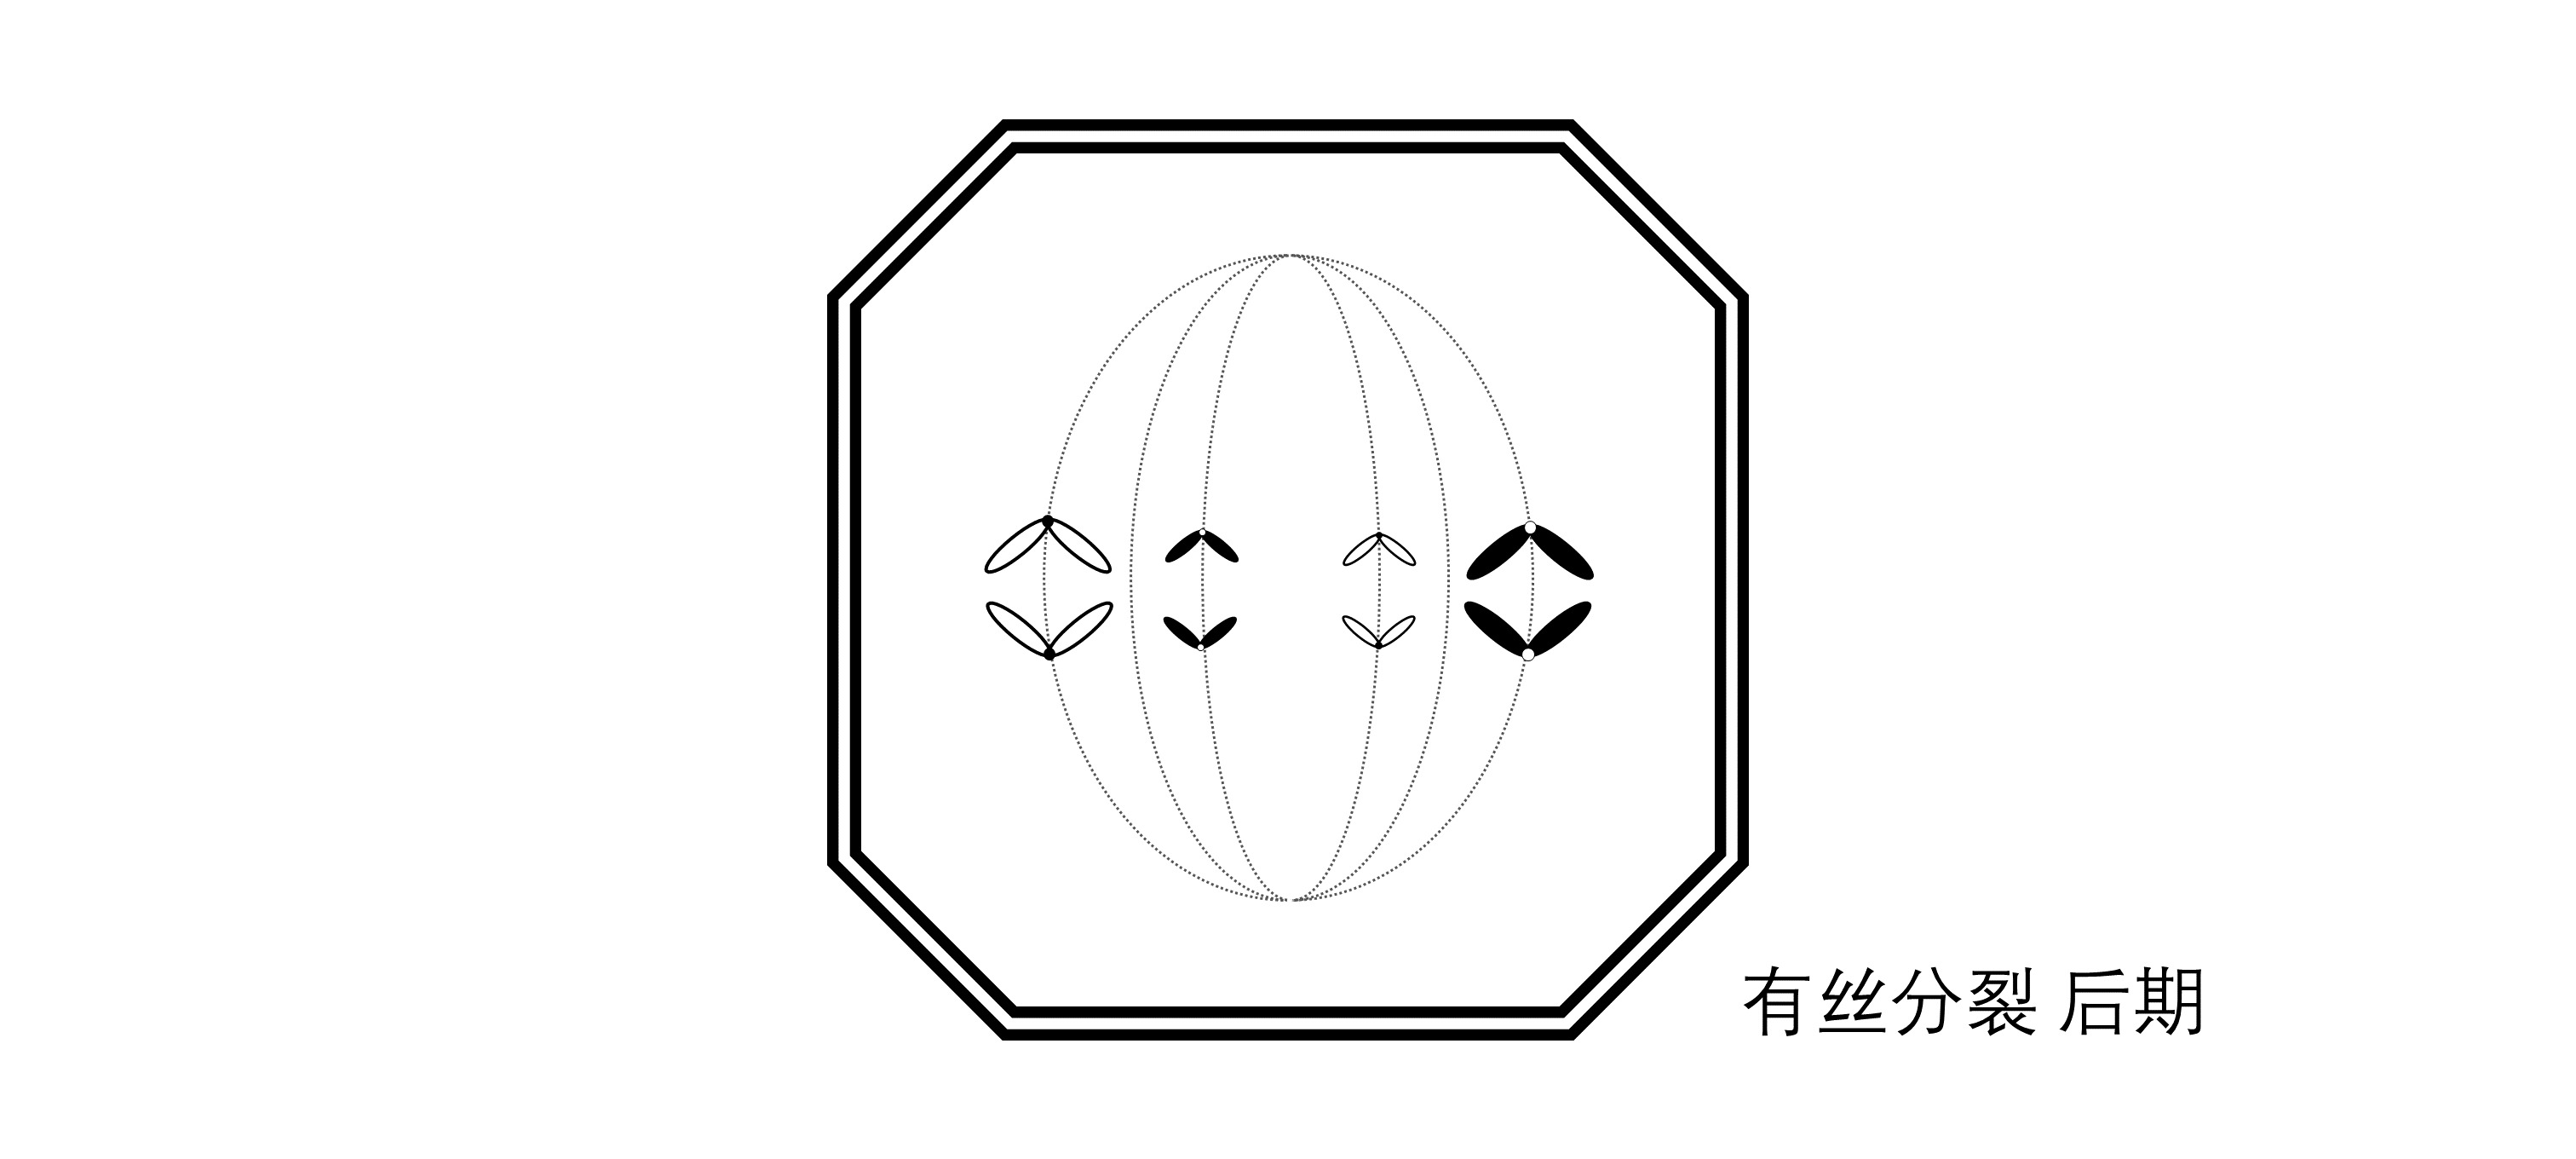
\includegraphics[width=10cm]{BiologyImage/27.jpg}
            \caption{植物的有丝分裂后期}
        \end{center}
    \end{figure}\\
    动物的有丝分裂后期:
    \begin{figure}[h]
        \begin{center}
            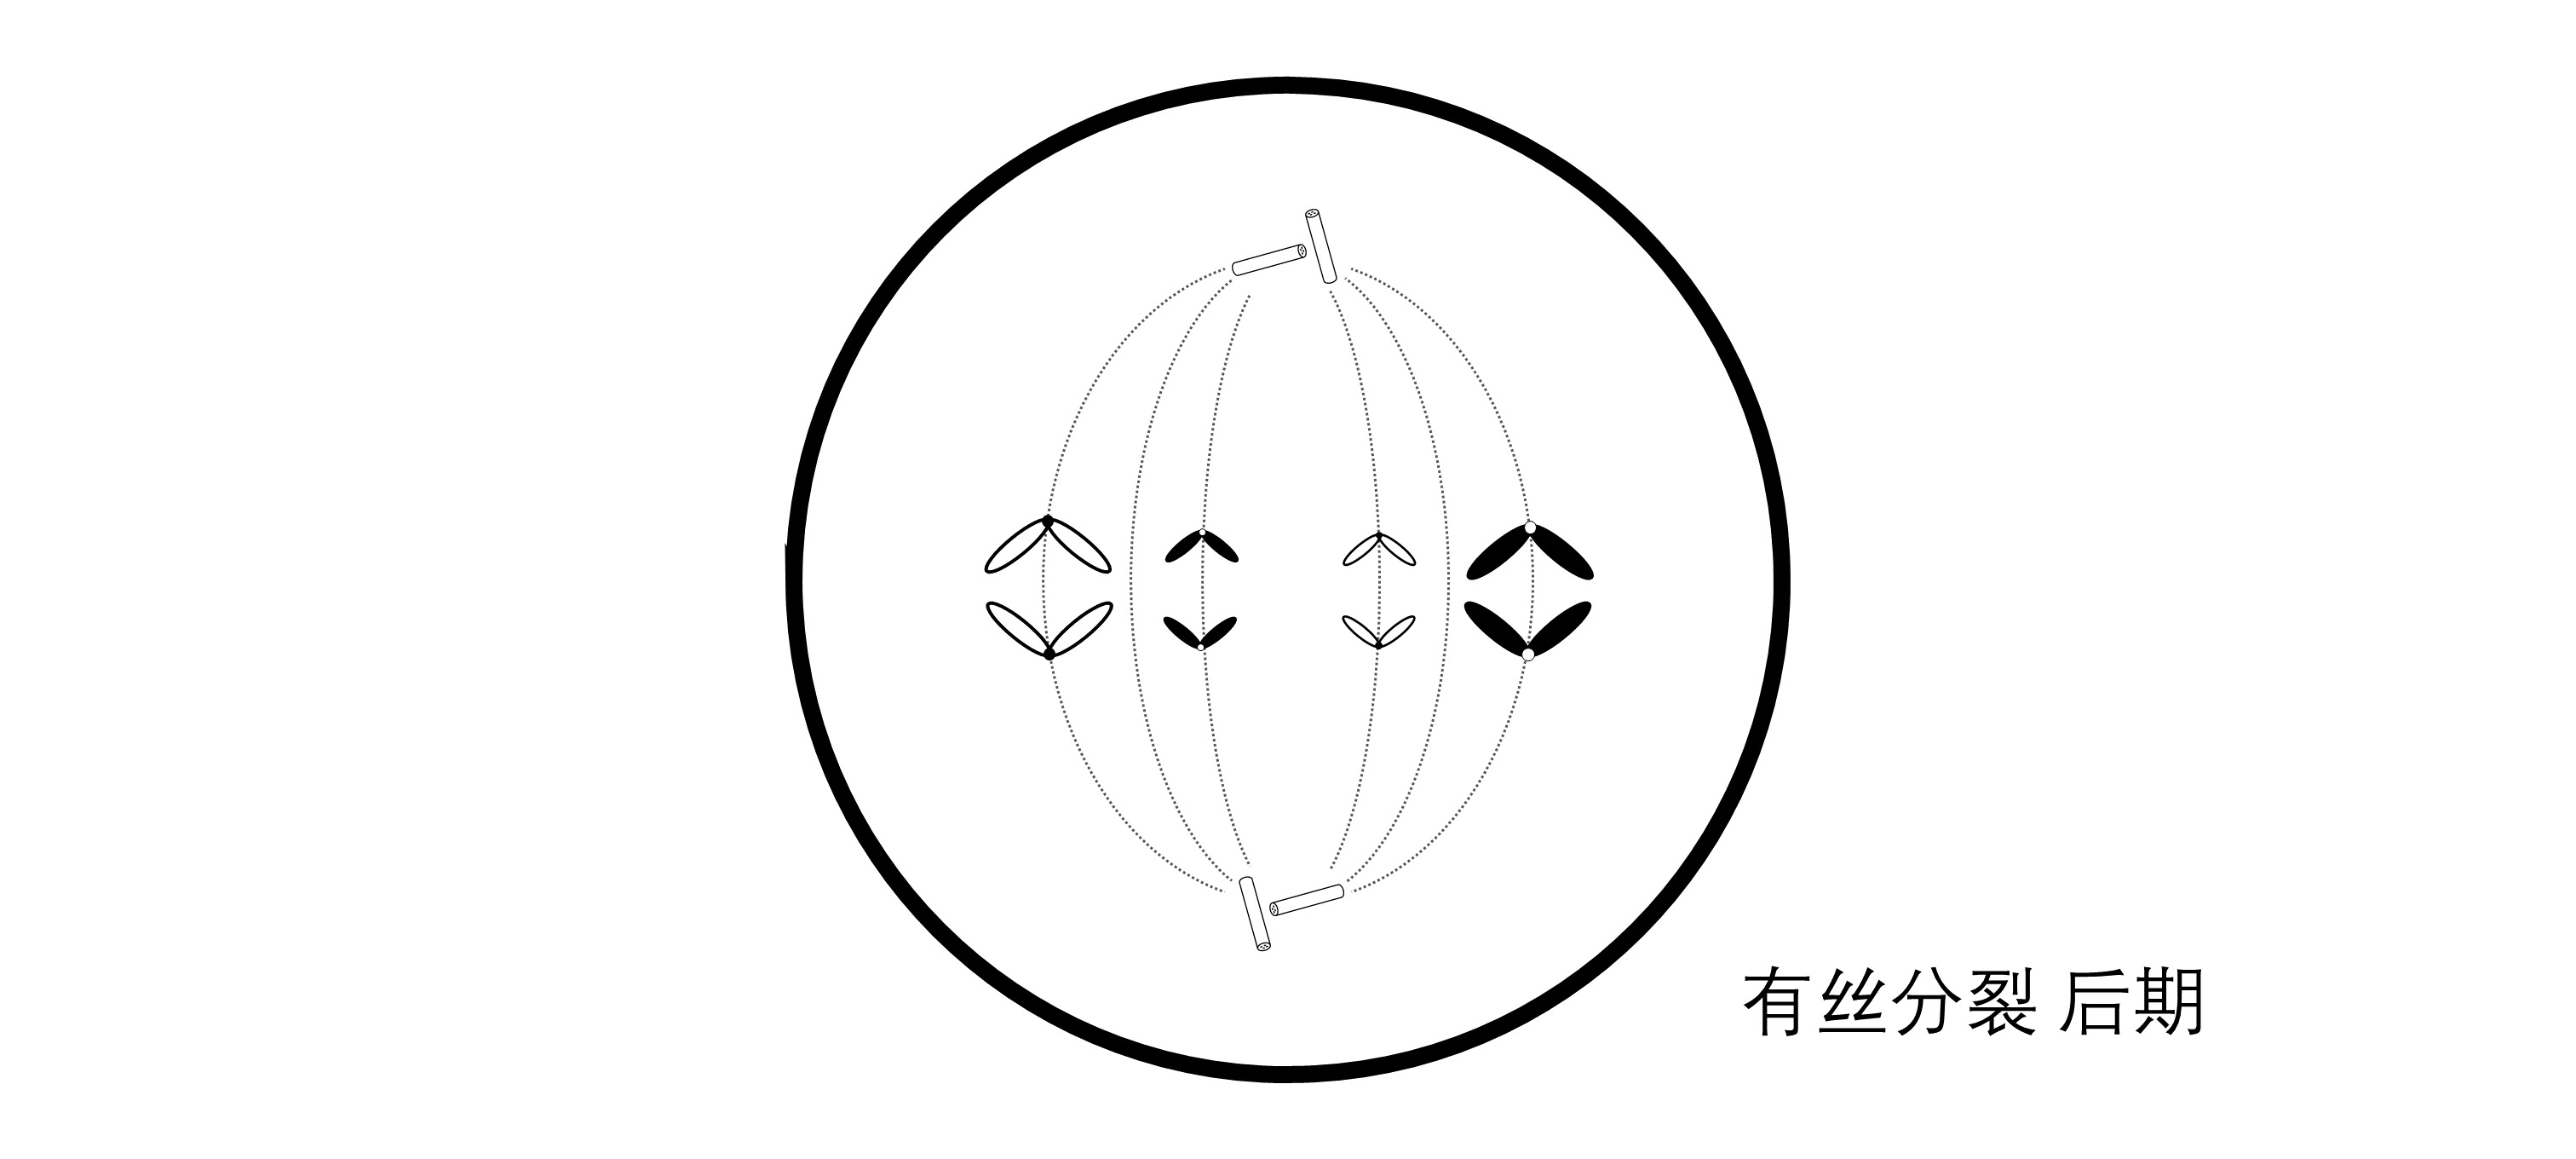
\includegraphics[width=10cm]{BiologyImage/32.jpg}
            \caption{动物的有丝分裂后期}
        \end{center}
    \end{figure}\\

\newpage

\subsubsection{有丝分裂末期}
    有丝分裂末期:当两组染色体分别移到细胞的两级之后,纺锤体逐渐消失,染色体逐渐解螺旋,
    变为细丝状的染色质,核仁核膜重新出现,形成两个新的细胞核。\\[3mm]
    对于植物细胞,赤道面会形成细胞板,最终变为细胞壁,成为两个新的细胞。\\[3mm]
    对于动物细胞,赤道面的细胞膜向内凹陷,最终缢缩为两个新的细胞。\\[6mm]
    植物的有丝分裂末期:
    \begin{figure}[h]
        \begin{center}
            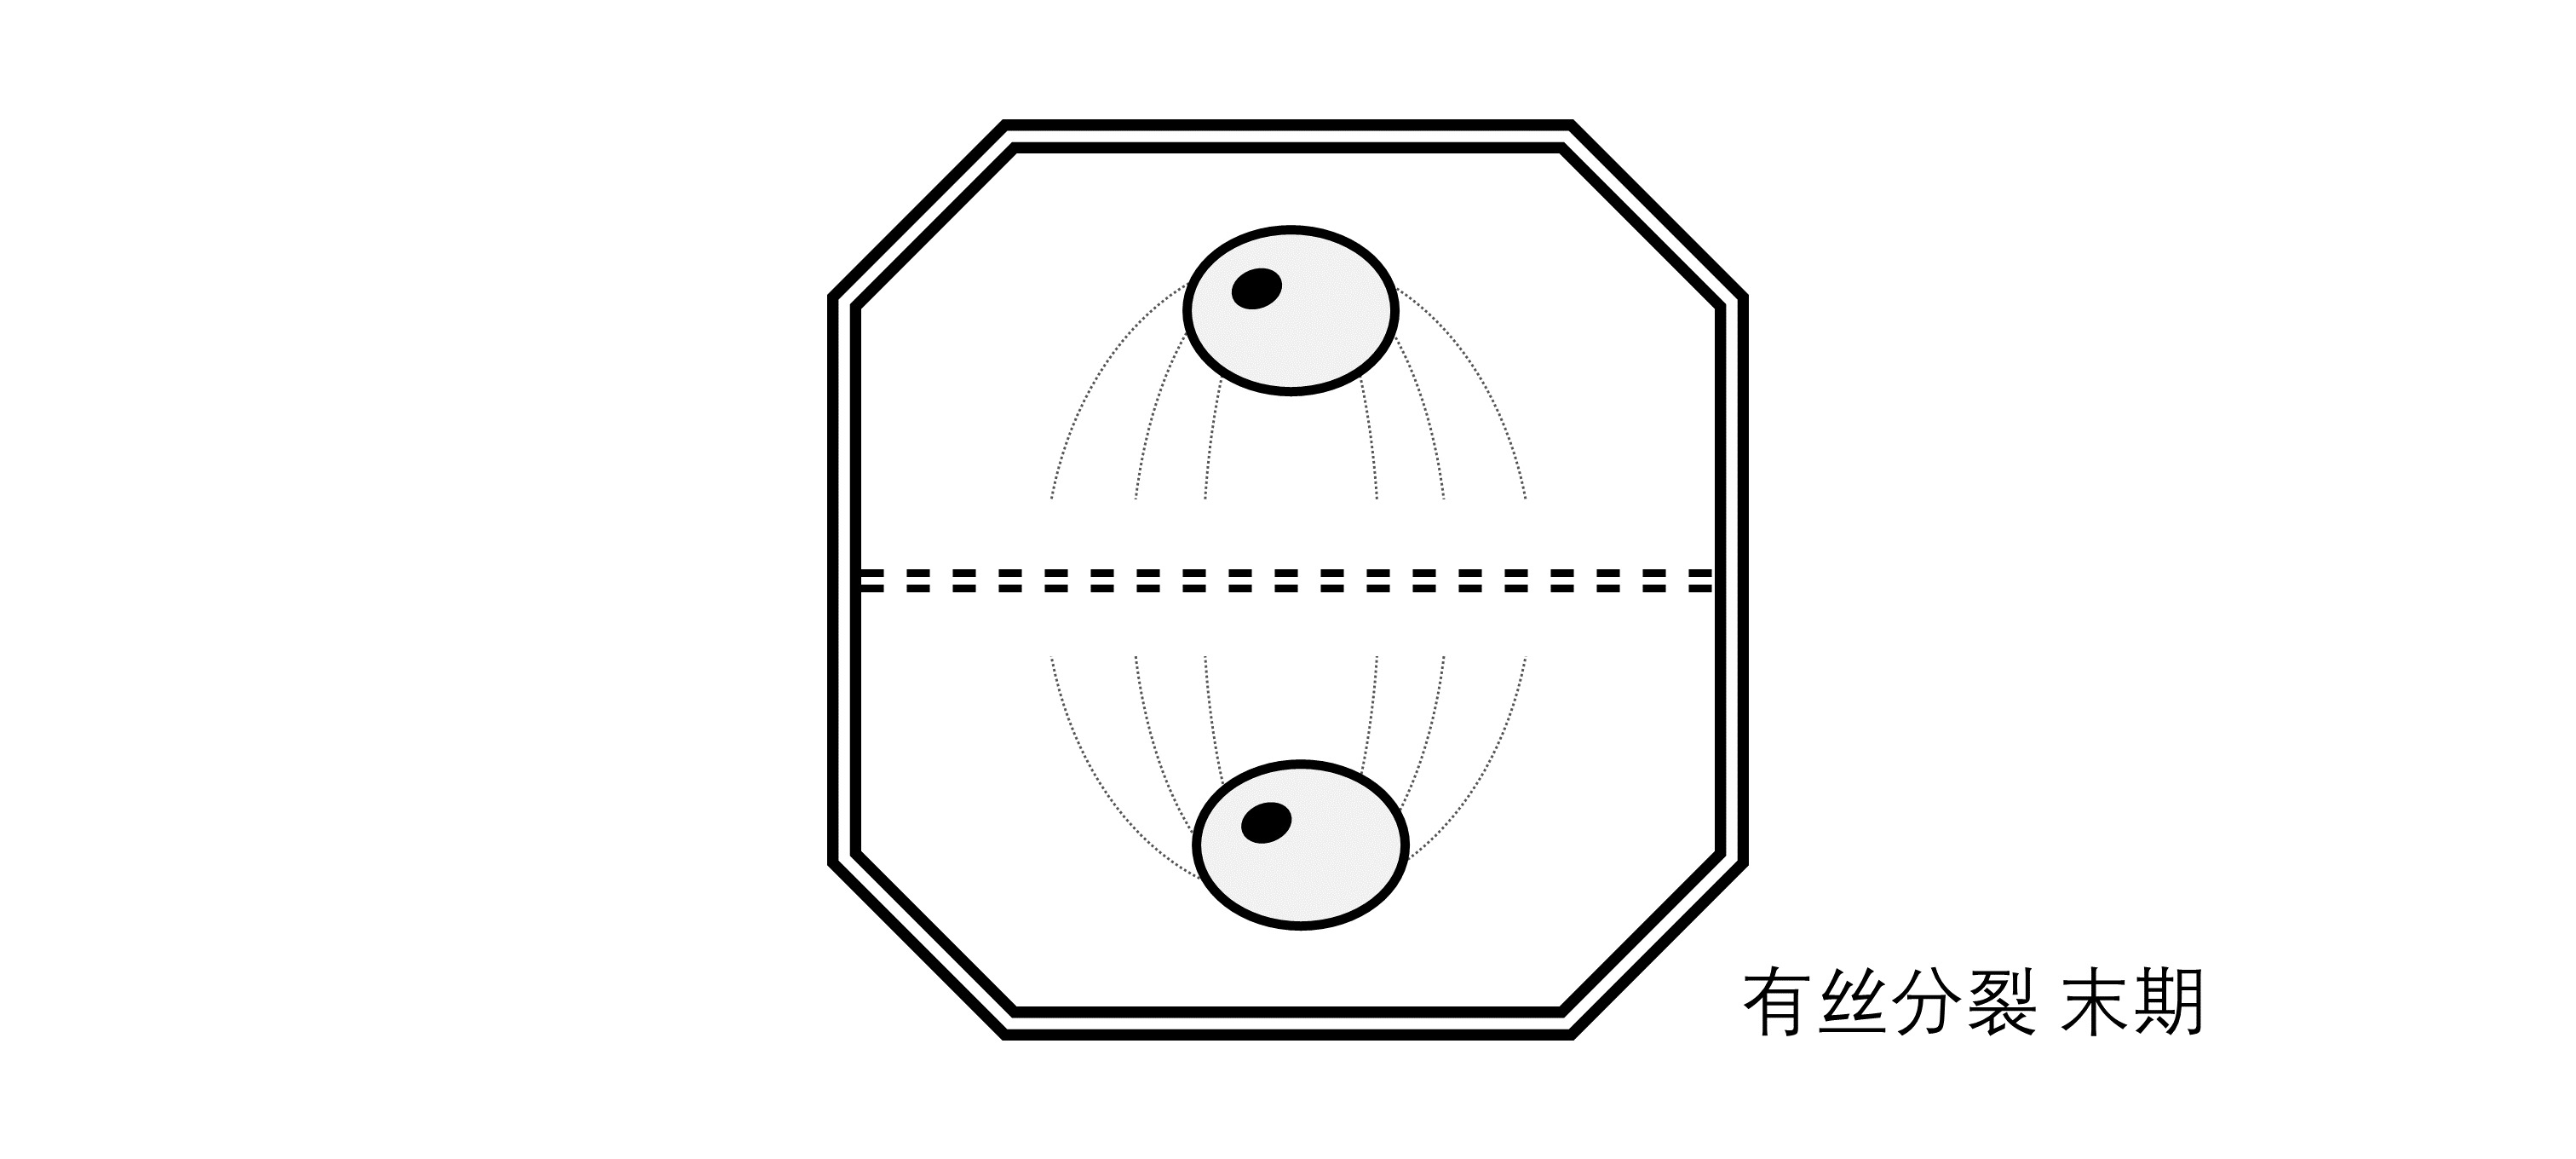
\includegraphics[width=10cm]{BiologyImage/28.jpg}
            \caption{植物的有丝分裂末期}
        \end{center}
    \end{figure}\\
    动物的有丝分裂末期:
    \begin{figure}[h]
        \begin{center}
            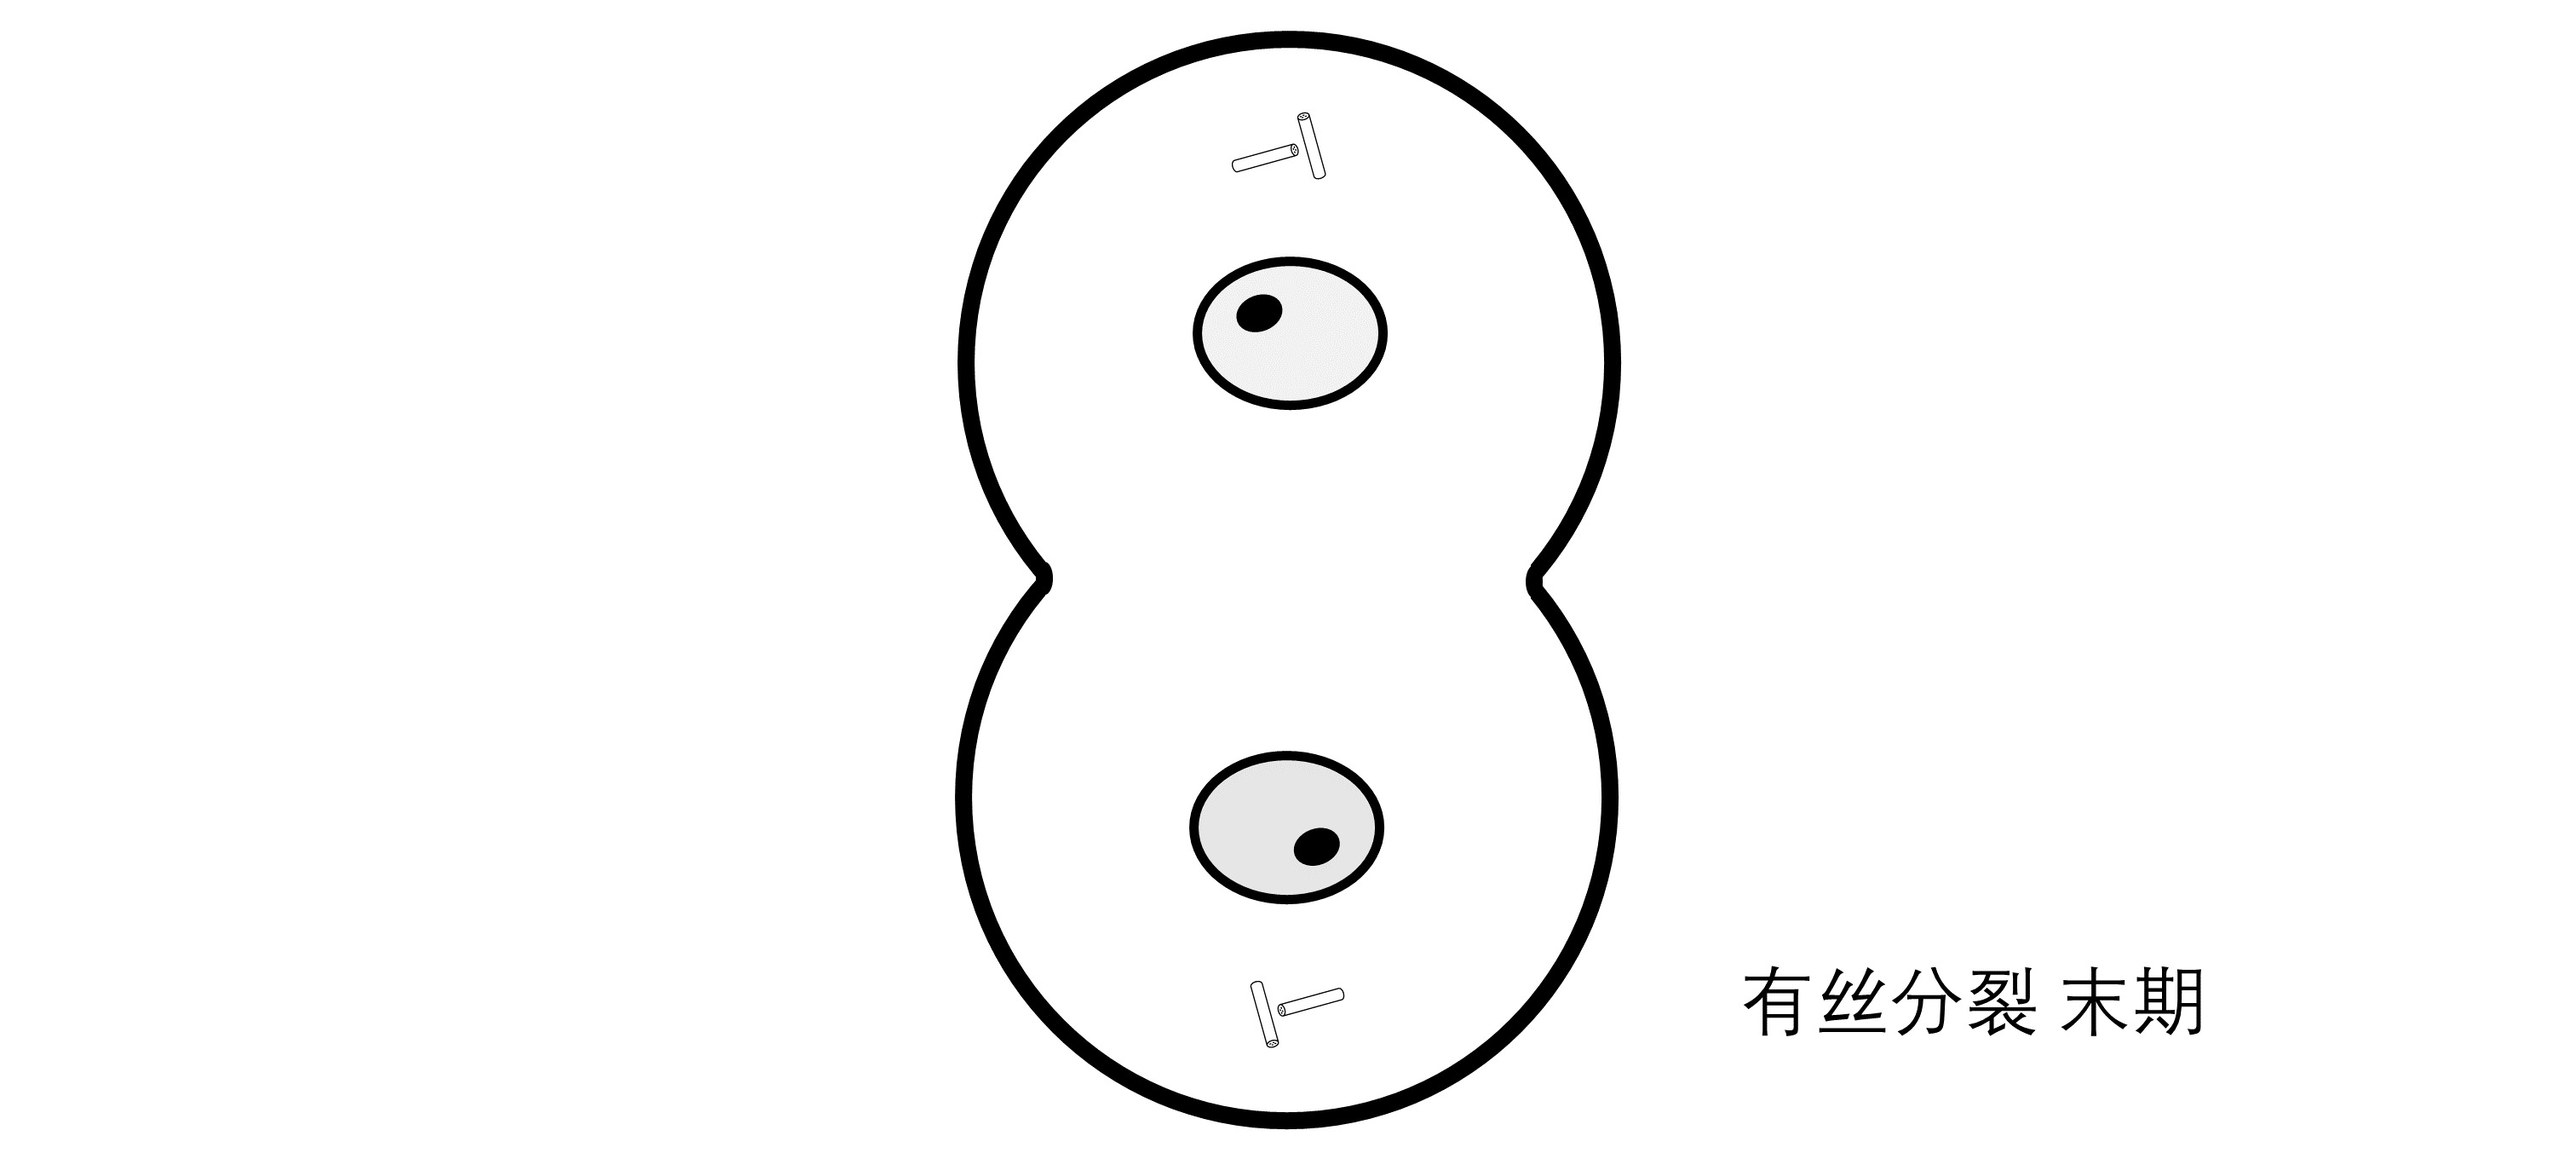
\includegraphics[width=10cm]{BiologyImage/33.jpg}
            \caption{动物的有丝分裂末期}
        \end{center}
    \end{figure}

\newpage

\subsection{减数分裂}
    减数分裂是形成生殖细胞的一种特殊分裂形式。\\[3mm]
    减数分裂由减数第一次分裂和减数第二次分裂两个连续的细胞分裂组成。\\[3mm]
    经过减数分裂,分裂期间DNA复制一次,产生四个遗传物质经重新组合的单倍体细胞,
    保证了精子和卵子在完成受精作用以后,子代的染色体数目与亲代的染色体数目相同。\\[6mm]
    下图展示了染色体间的关系:
    \begin{figure}[h]
        \begin{center}
            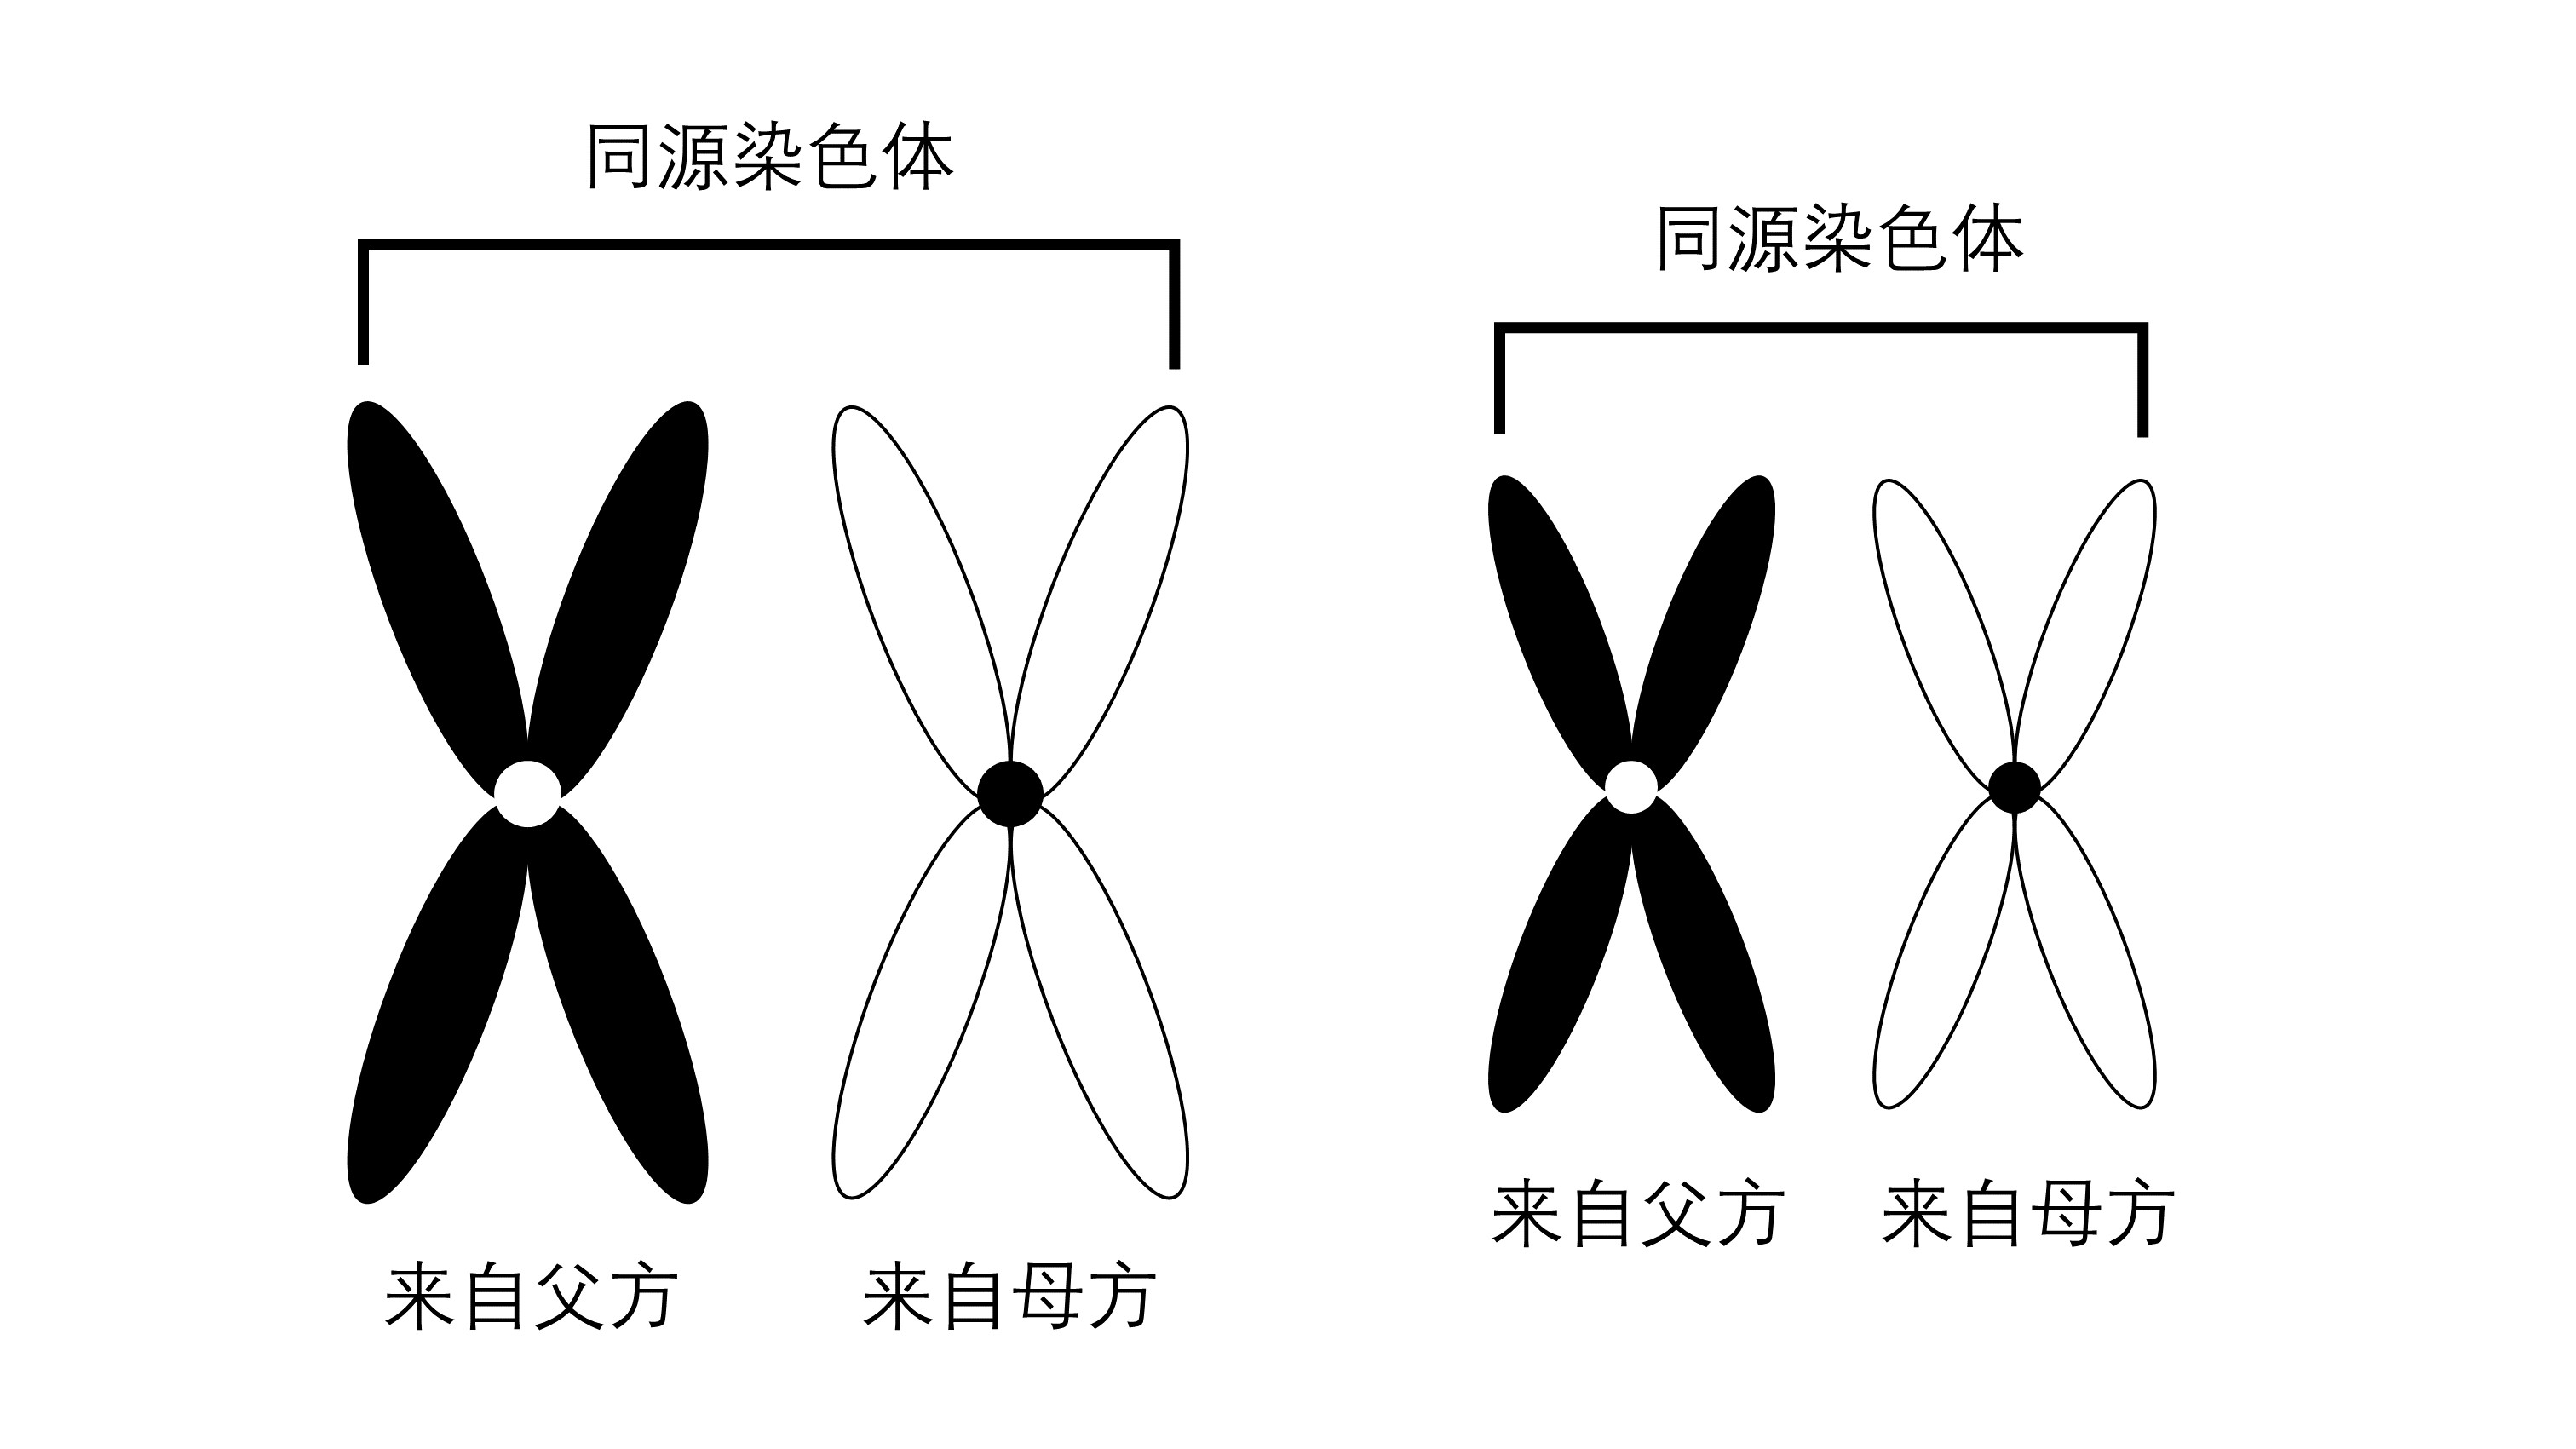
\includegraphics[width=10cm]{BiologyImage/44.jpg}
            \caption{染色体间的关系}
        \end{center}
    \end{figure}\\
    下图展示了染色单体间的关系:
    \begin{figure}[h]
        \begin{center}
            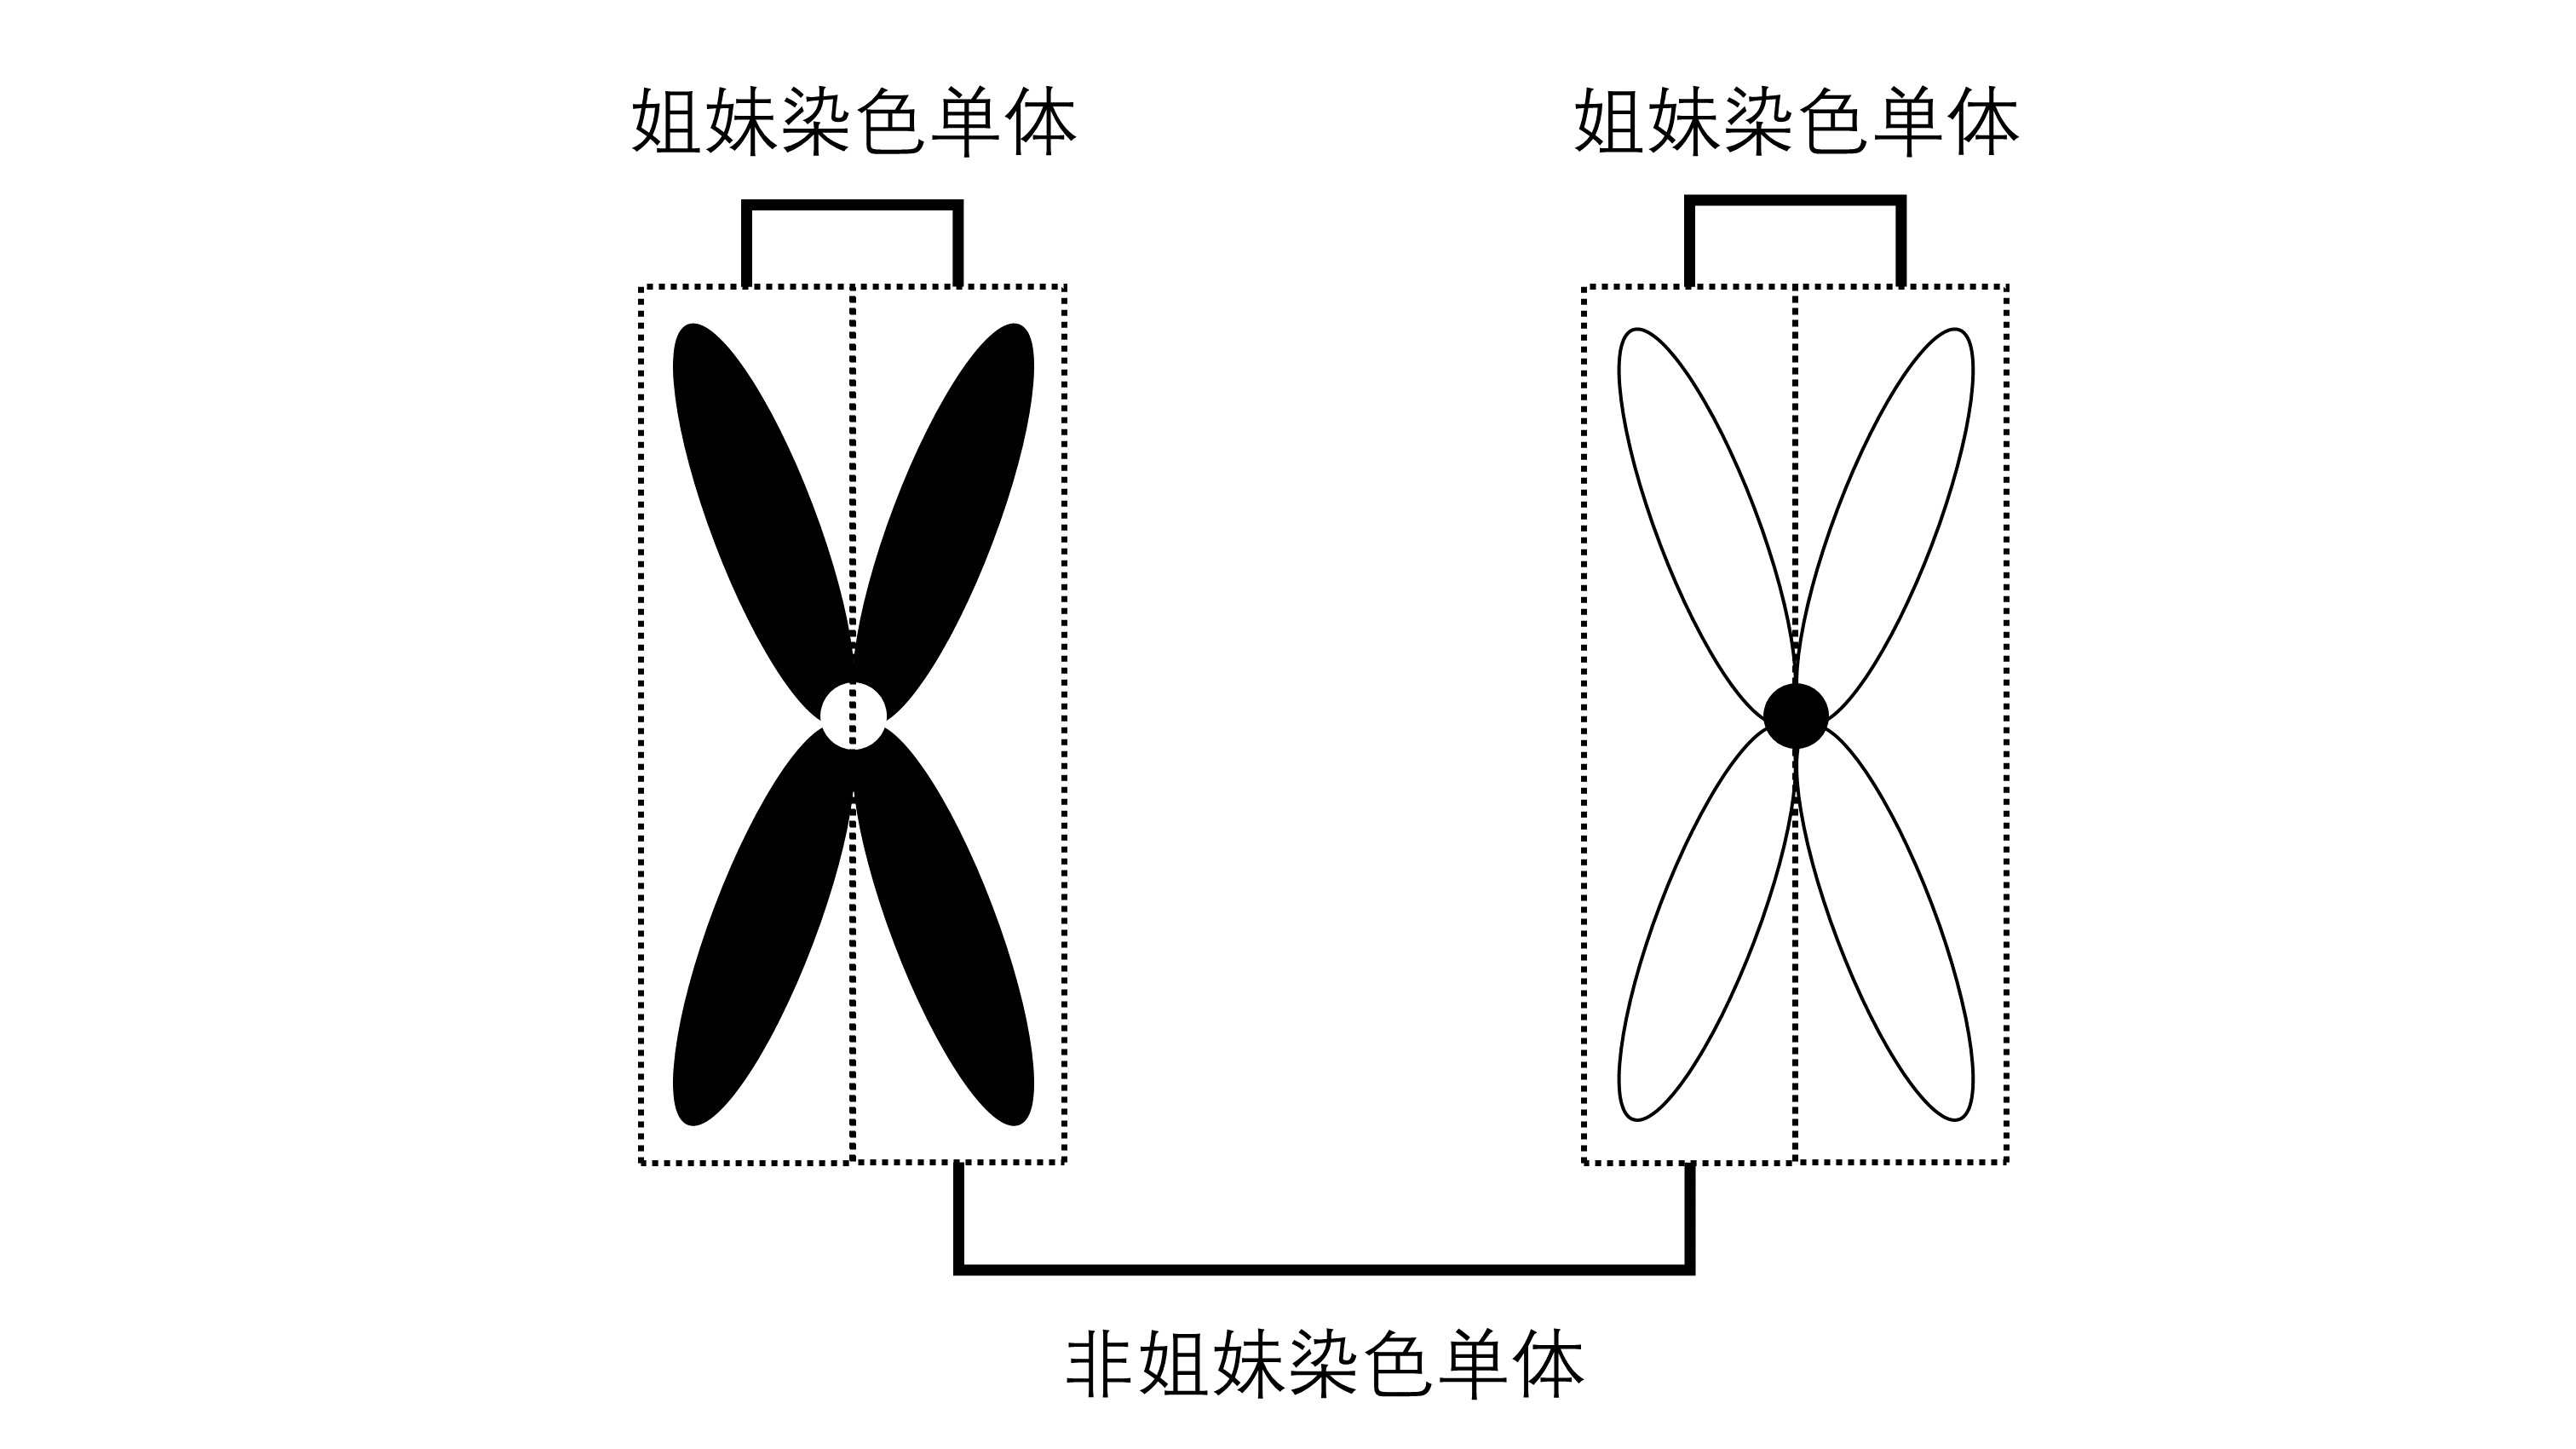
\includegraphics[width=10cm]{BiologyImage/45.jpg}
            \caption{染色单体间的关系}
        \end{center}
    \end{figure}\\

\newpage

\subsubsection{减数第一次分裂间期}
    减数第一次分裂间期:该间期时间相对较长,这是由于需要进行染色体的复制。\\[4mm]
    减数第一次分裂间期:
    \begin{figure}[h]
        \begin{center}
            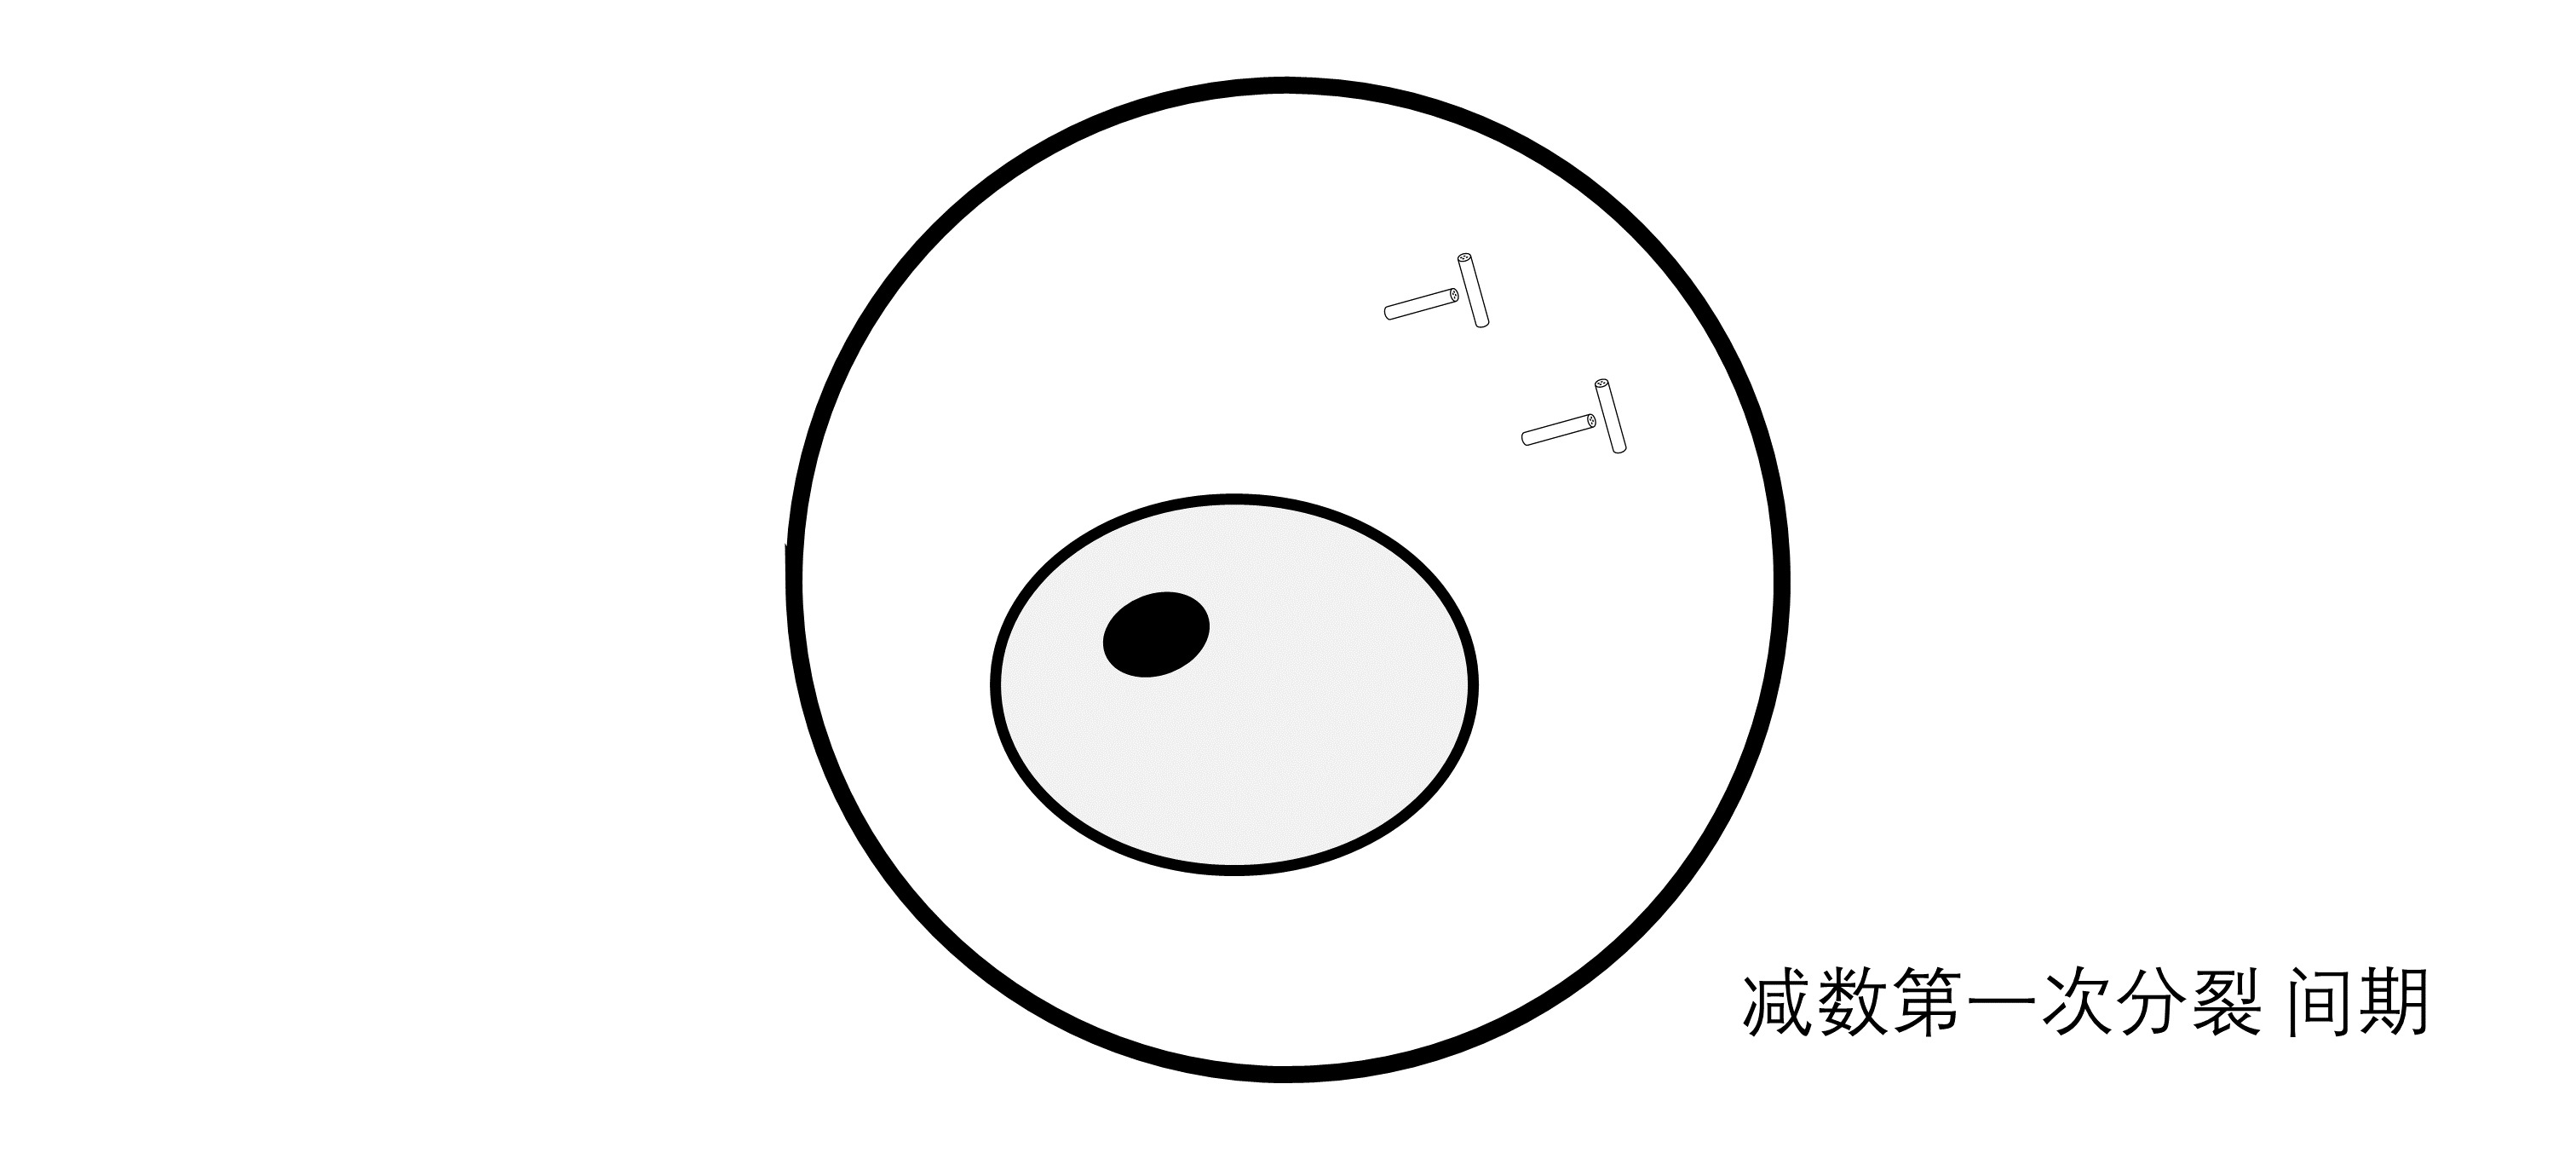
\includegraphics[width=10cm]{BiologyImage/34.jpg}
            \caption{减数第一次分裂间期}
        \end{center}
    \end{figure}

\subsubsection{减数第一次分裂前期}
    减数第一次分裂前期:分别来自父方和母方,形状大小相同的同源染色体,两两配对进行联会。\\[4mm]
    减数第一次分裂前期:
    \begin{figure}[h]
        \begin{center}
            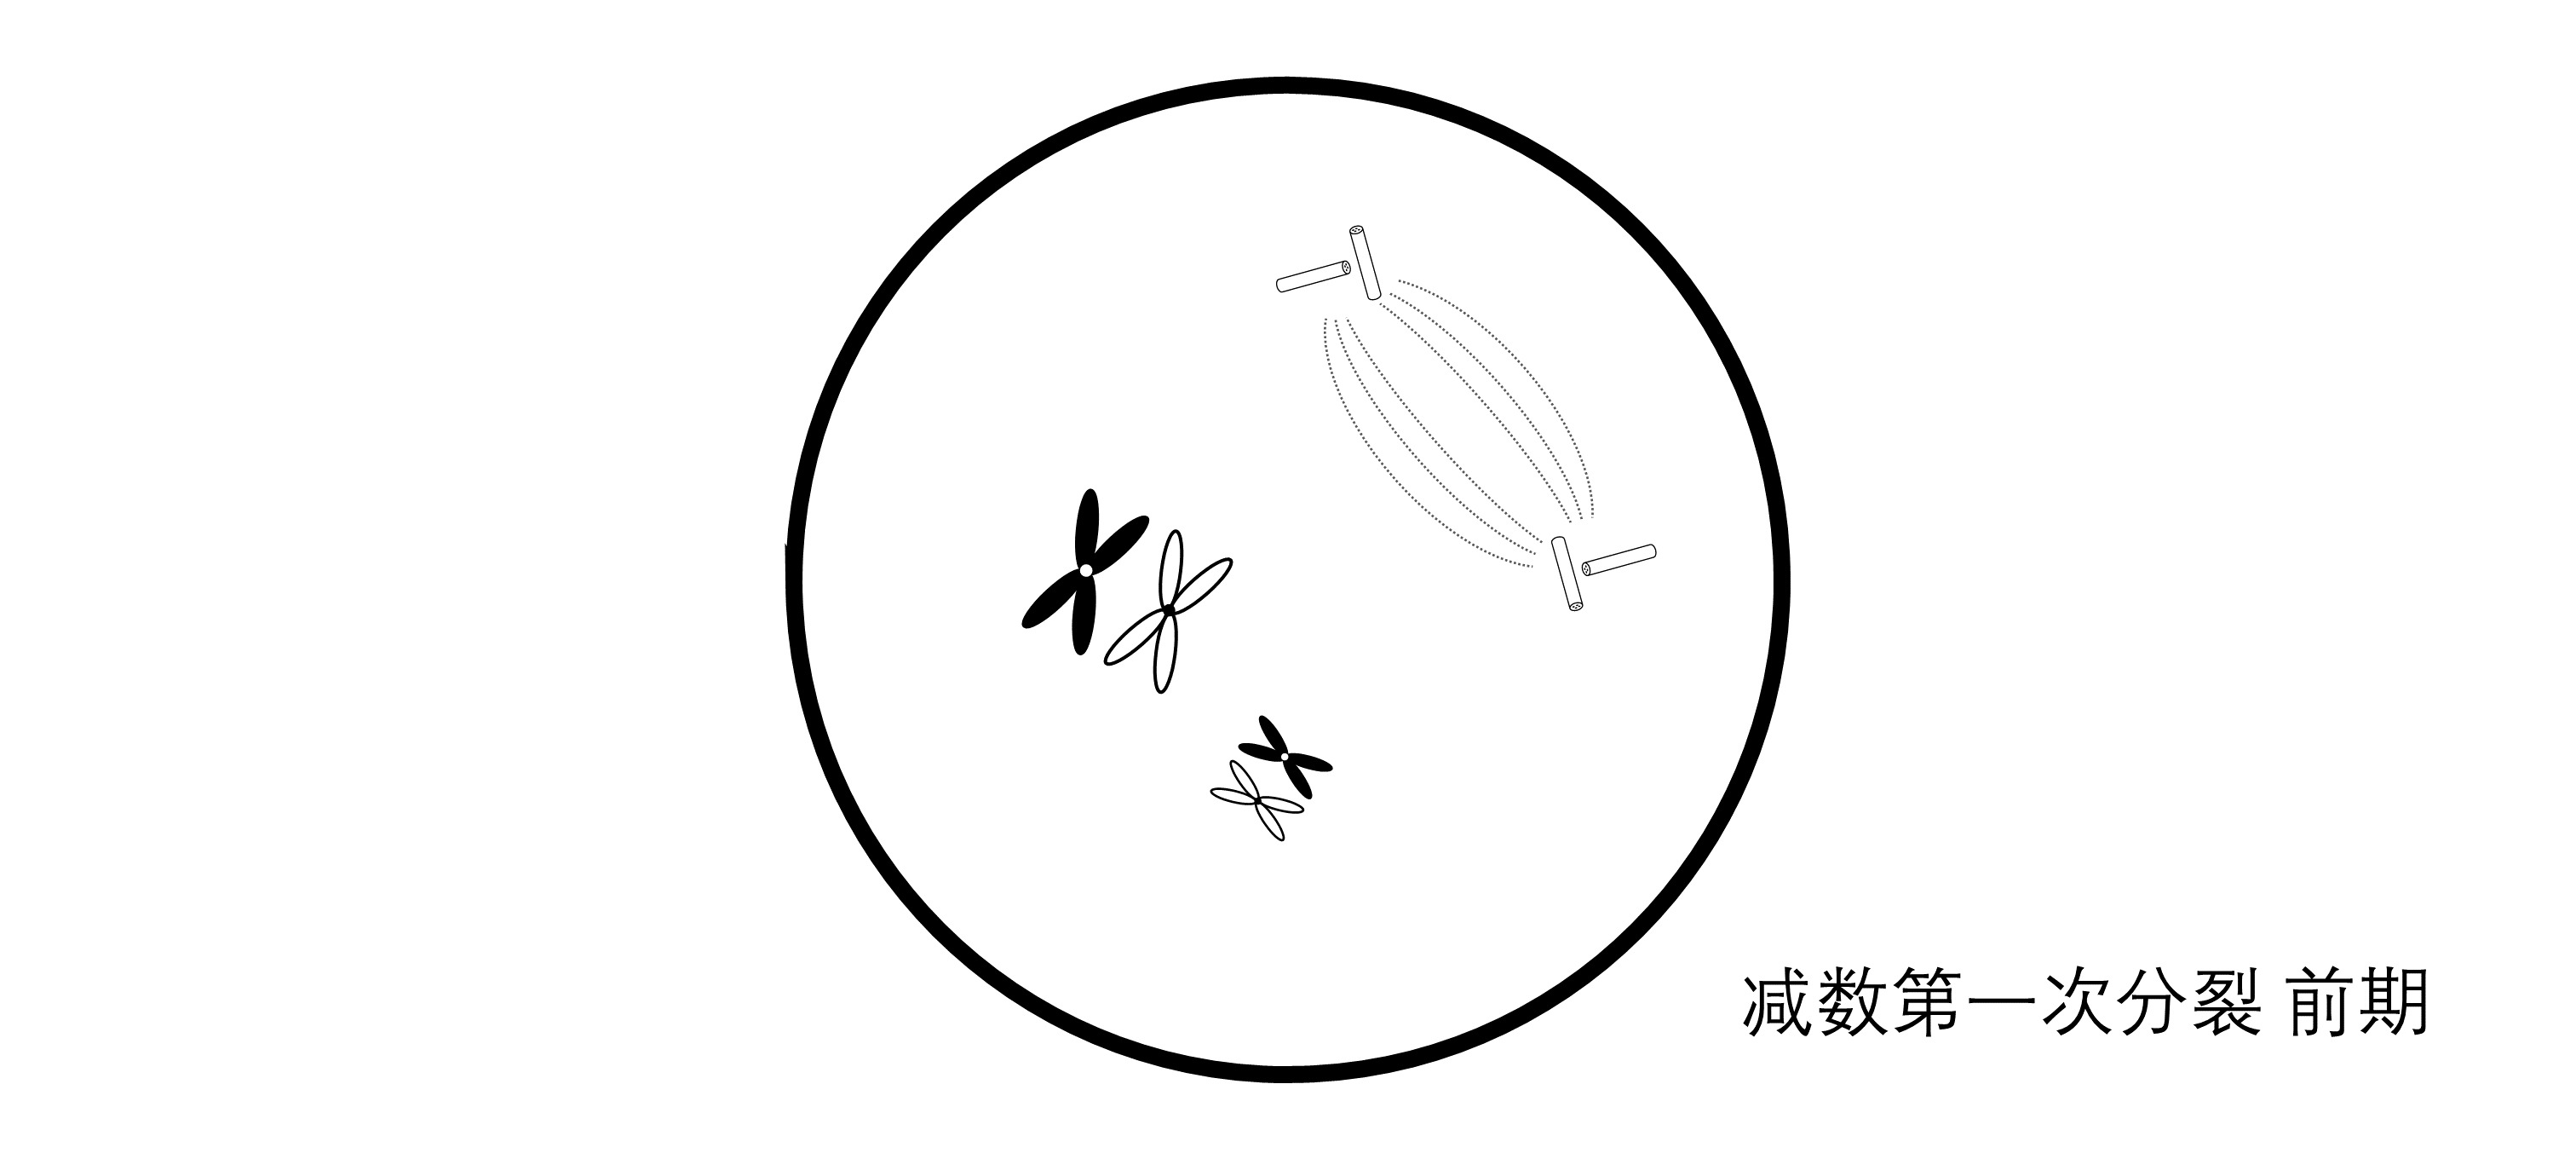
\includegraphics[width=10cm]{BiologyImage/35.jpg}
            \caption{减数第一次分裂前期}
        \end{center}
    \end{figure}

\newpage

\subsubsection{减数第一次分裂中期}
    减数第一次分裂中期:着丝粒与纺锤丝相连,成对的同源染色体在纺锤丝的牵引下排列赤道面。\\[4mm]
    减数第一次分裂中期:
    \begin{figure}[h]
        \begin{center}
            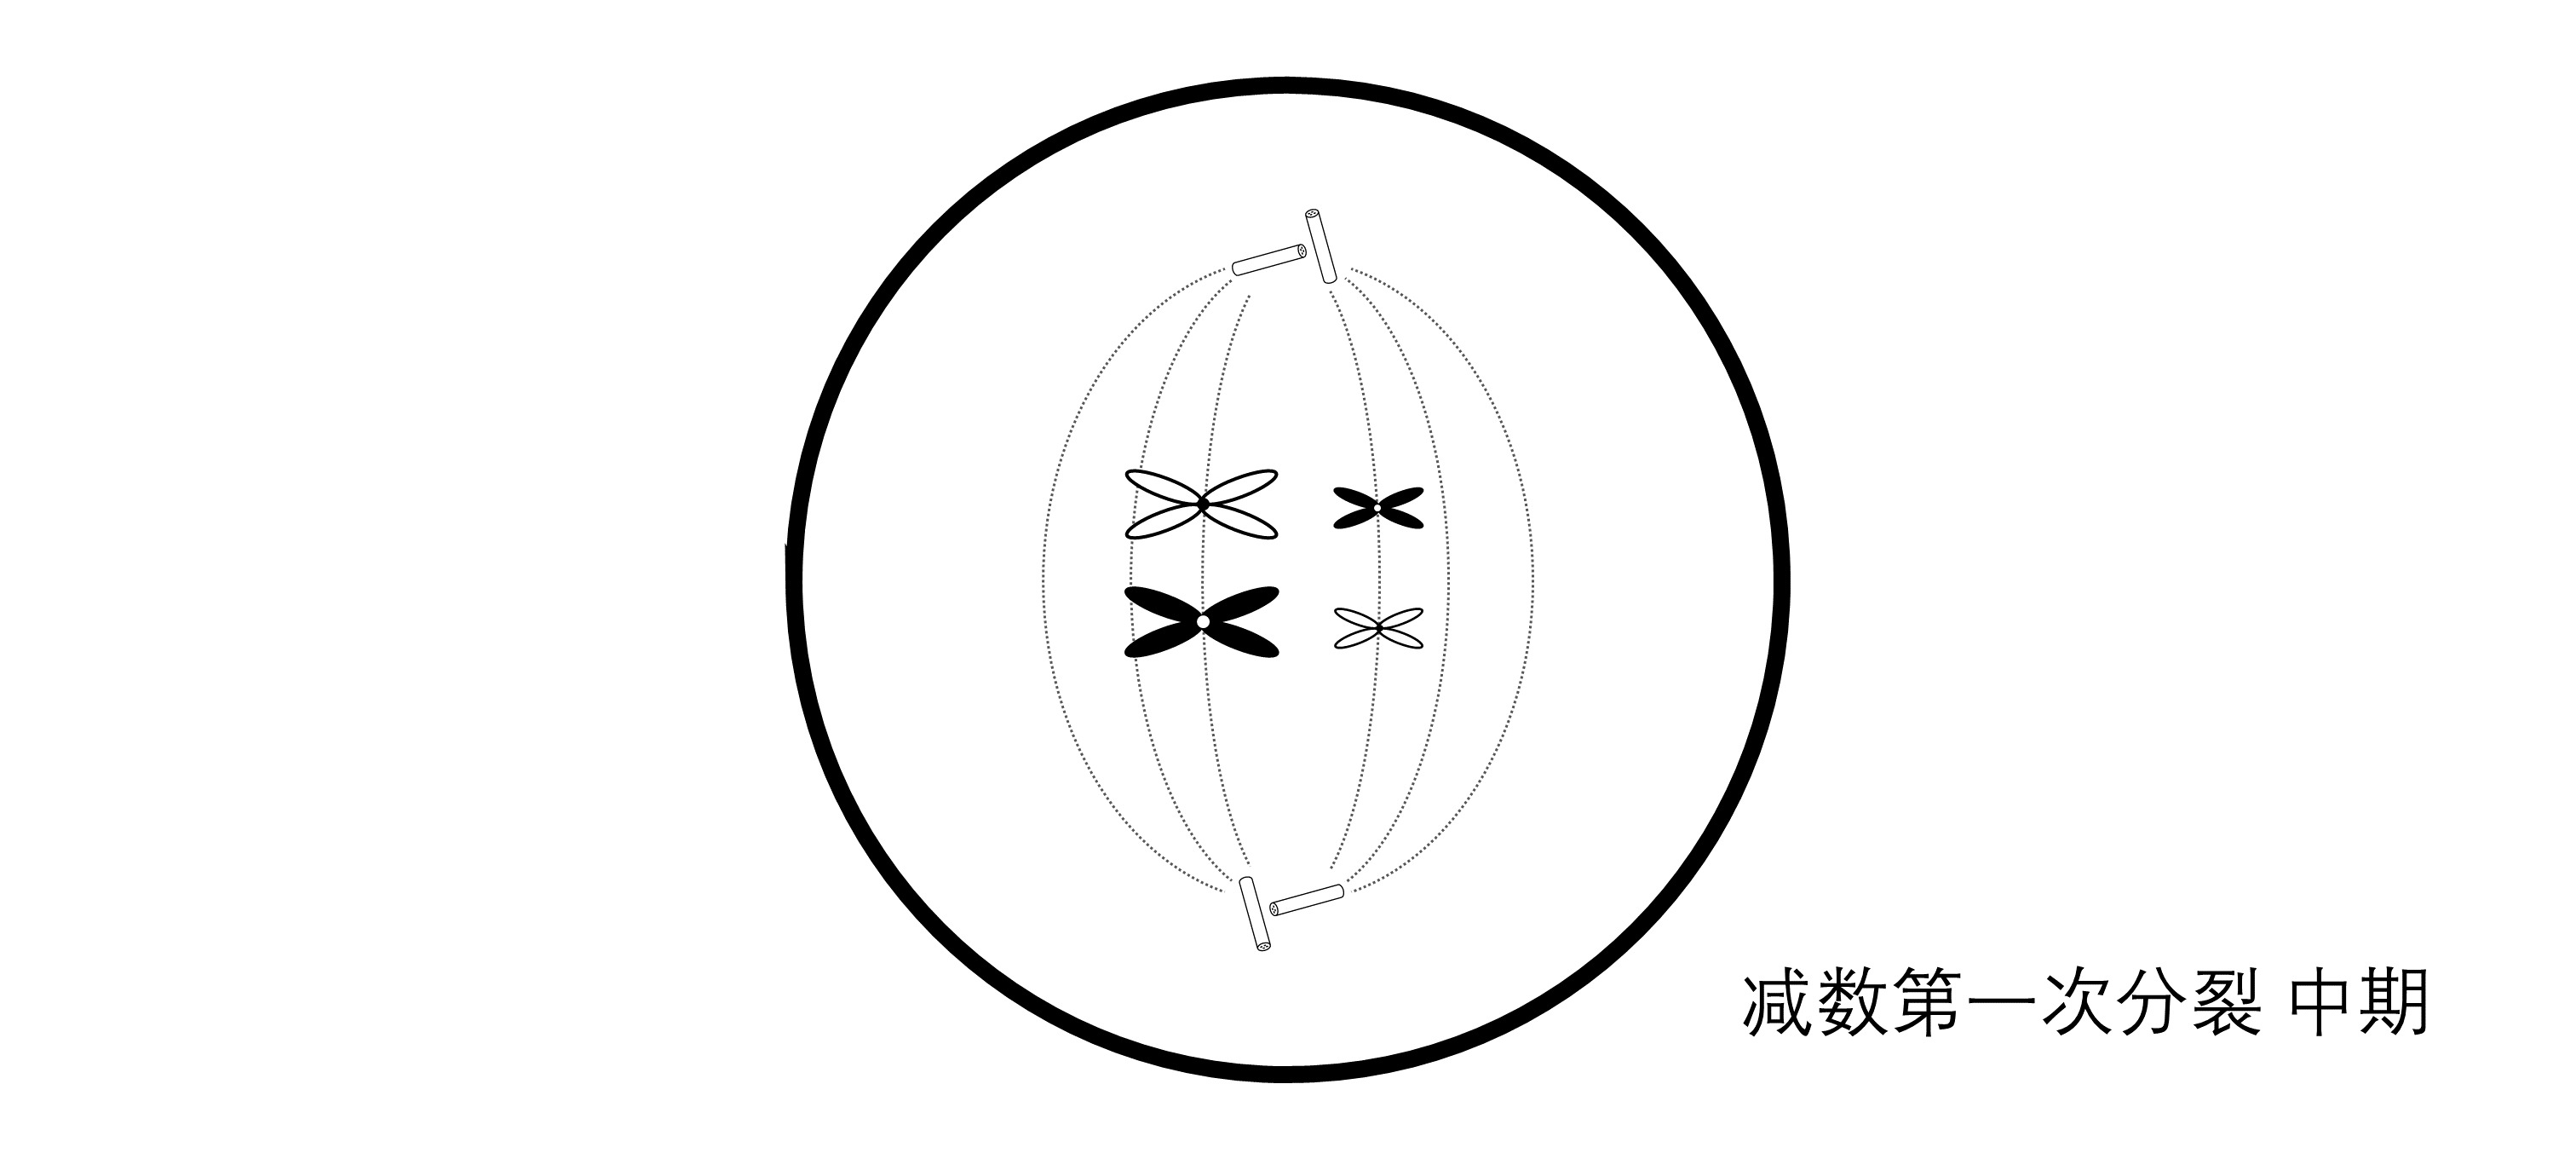
\includegraphics[width=10cm]{BiologyImage/36.jpg}
            \caption{减数第一次分裂中期}
        \end{center}
    \end{figure}

\subsubsection{减数第一次分裂后期}
    减数第一次分裂后期:随着纺锤丝的牵引,同源染色体分离,分别移向细胞两级。\\[4mm]
    减数第一次分裂后期:
    \begin{figure}[h]
        \begin{center}
            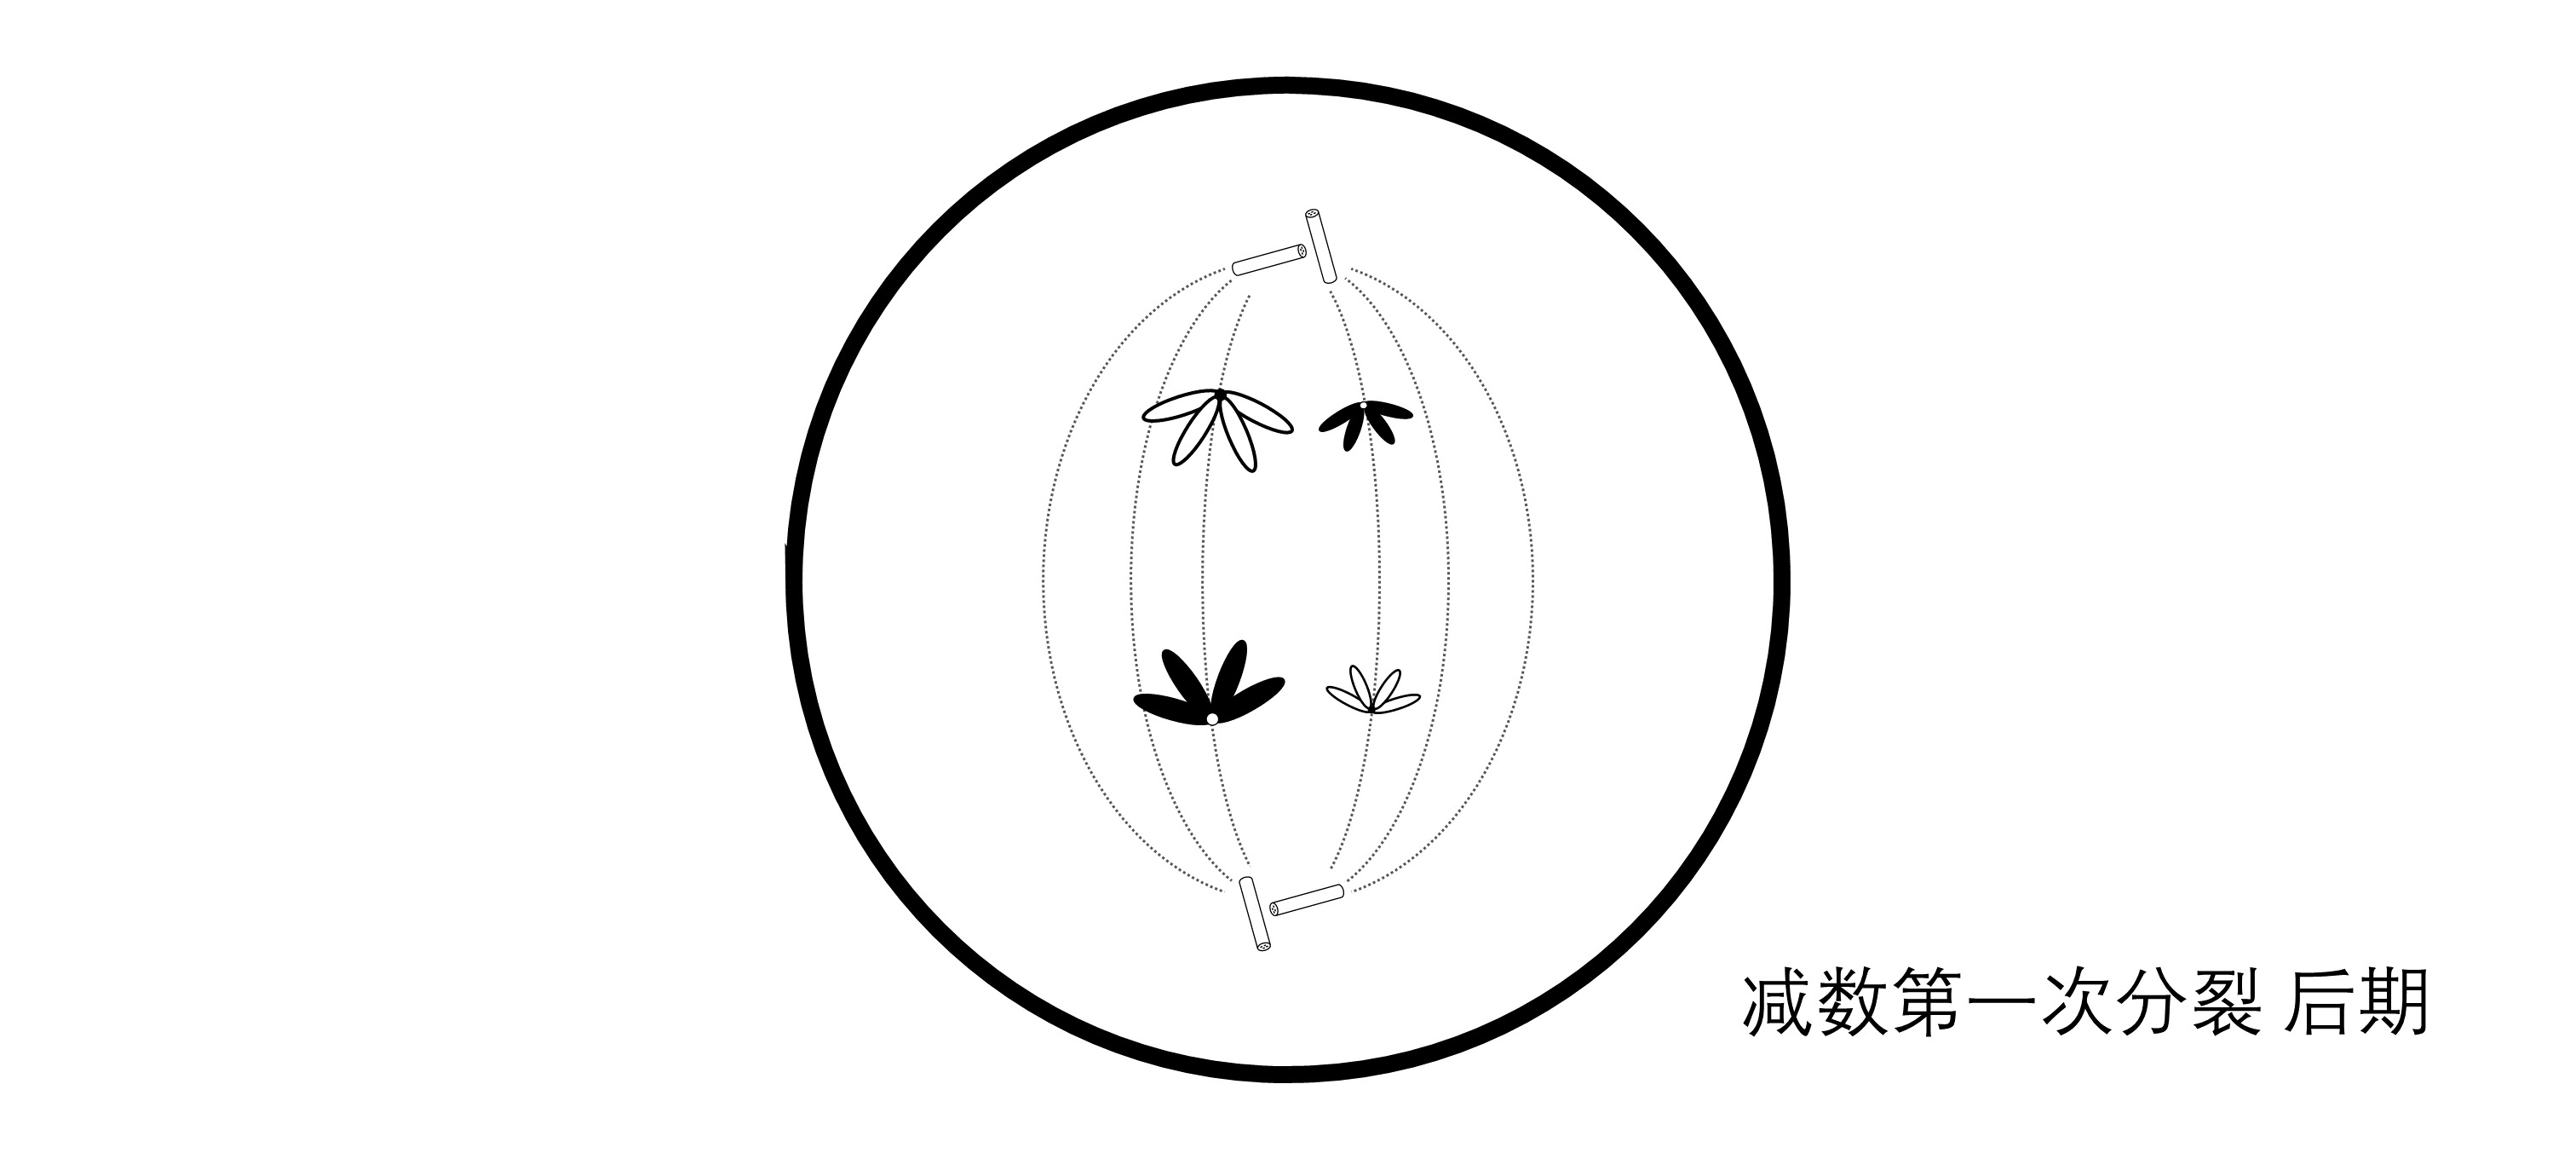
\includegraphics[width=10cm]{BiologyImage/37.jpg}
            \caption{减数第一次分裂后期}
        \end{center}
    \end{figure}

\newpage

\subsubsection{减数第一次分裂末期}
    减数第一次分裂末期:当两组染色体分别移到细胞两级之后,细胞分裂为两个子细胞。\\[4mm]
    减数第一次分裂末期:
    \begin{figure}[h]
        \begin{center}
            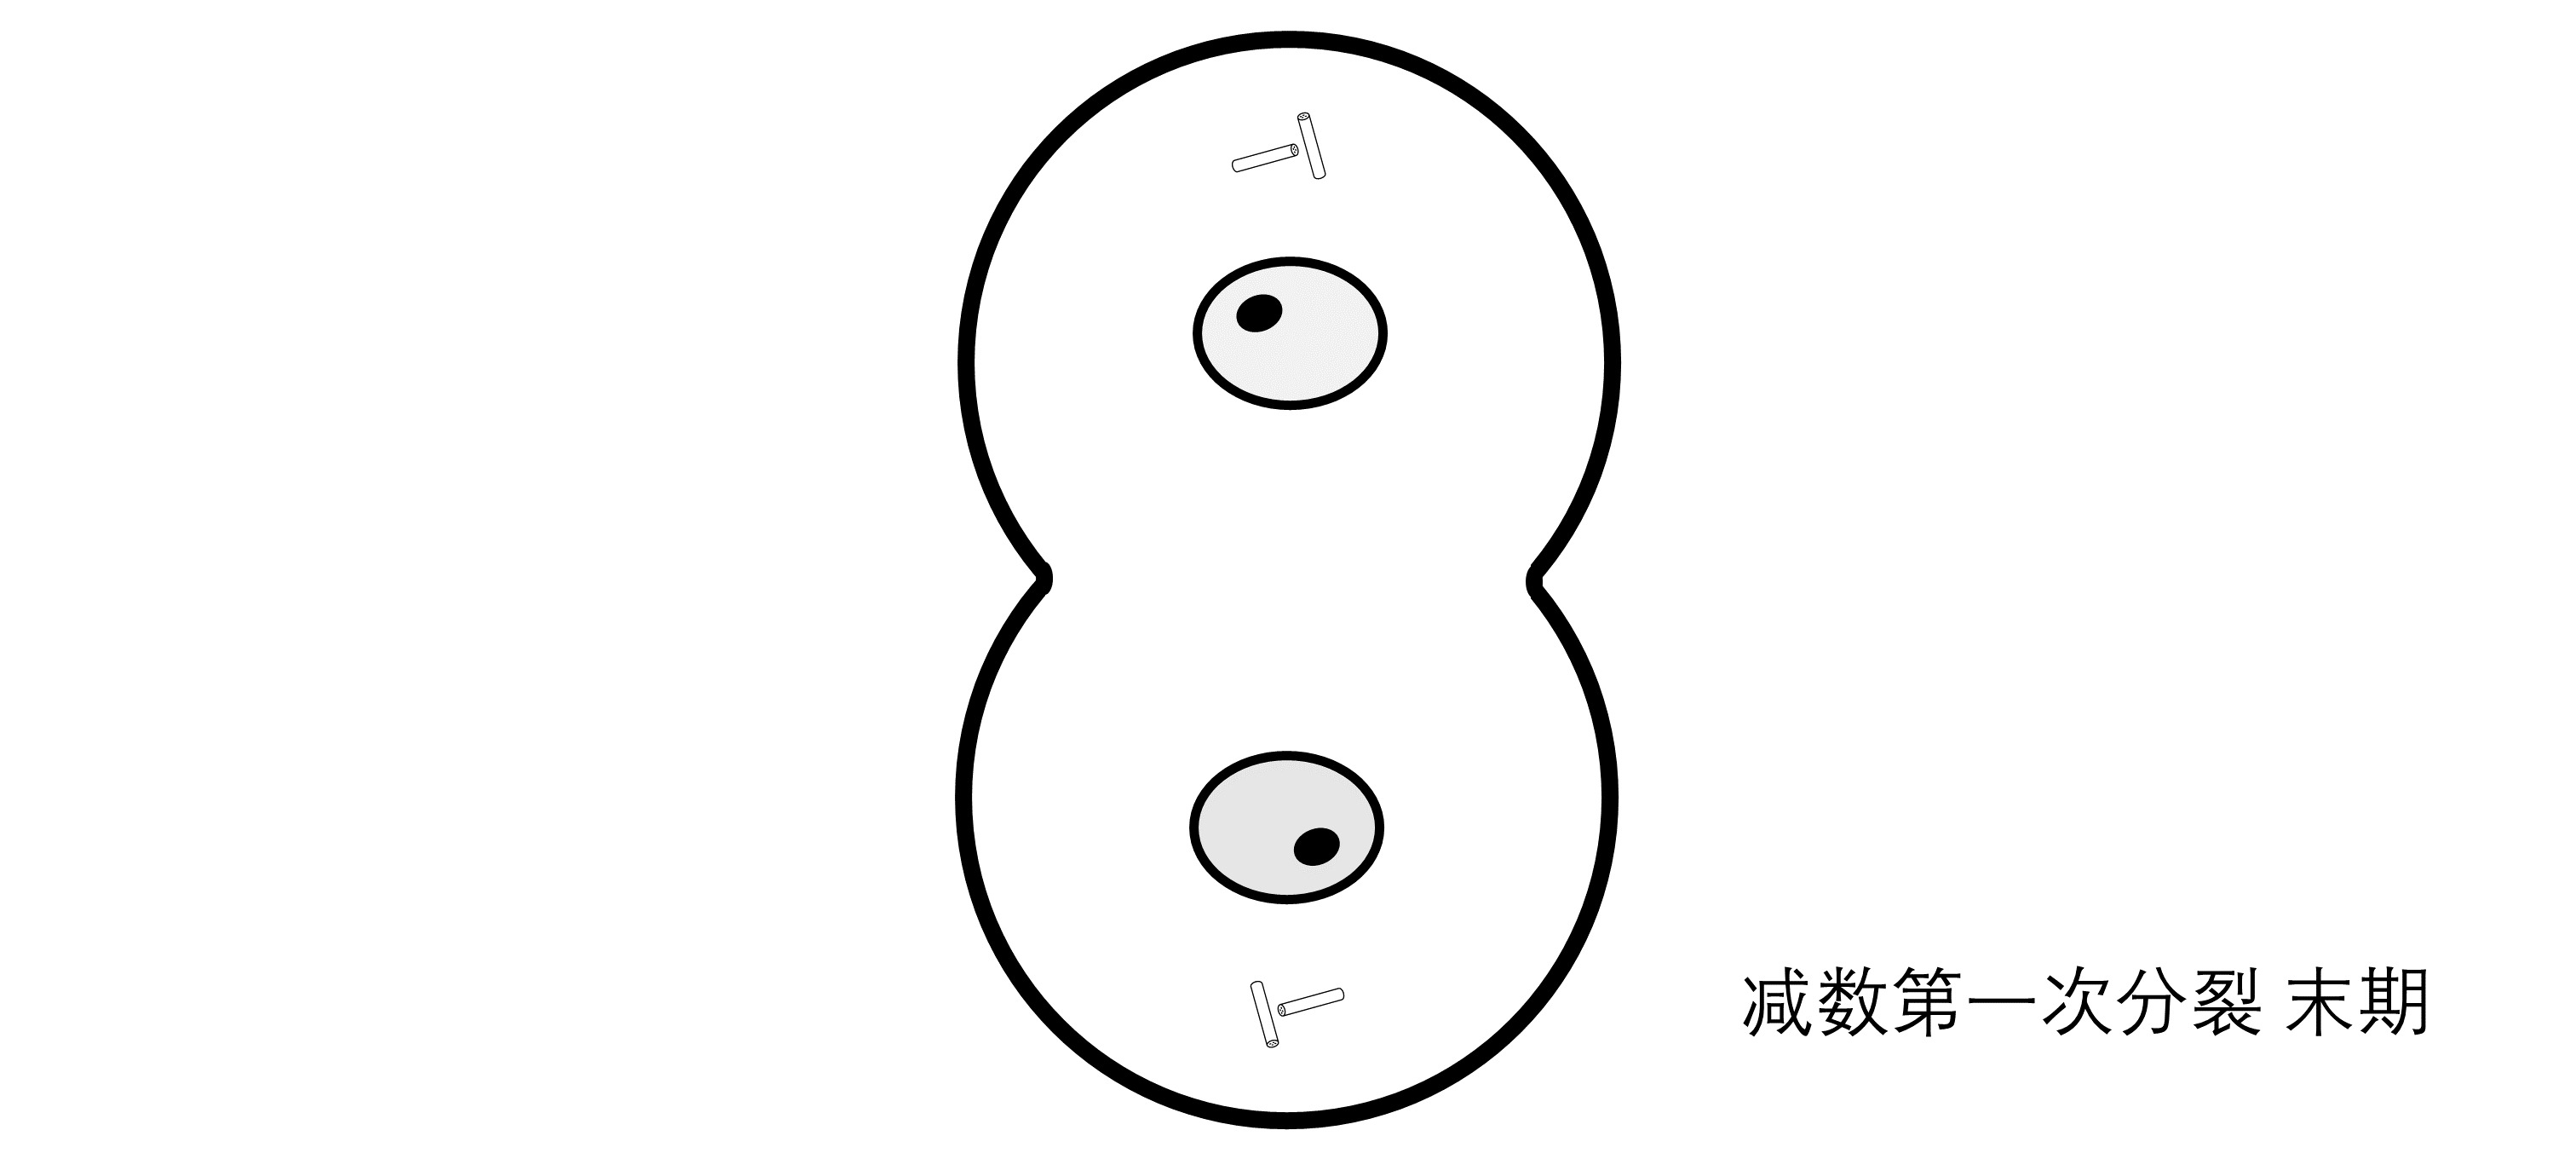
\includegraphics[width=10cm]{BiologyImage/38.jpg}
            \caption{减数第一次分裂末期}
        \end{center}
    \end{figure}\\

\subsubsection{减数第一次分裂后的染色质状况}
    减数第一次分裂后的染色质状况:
    \begin{figure}[h]
        \begin{center}
            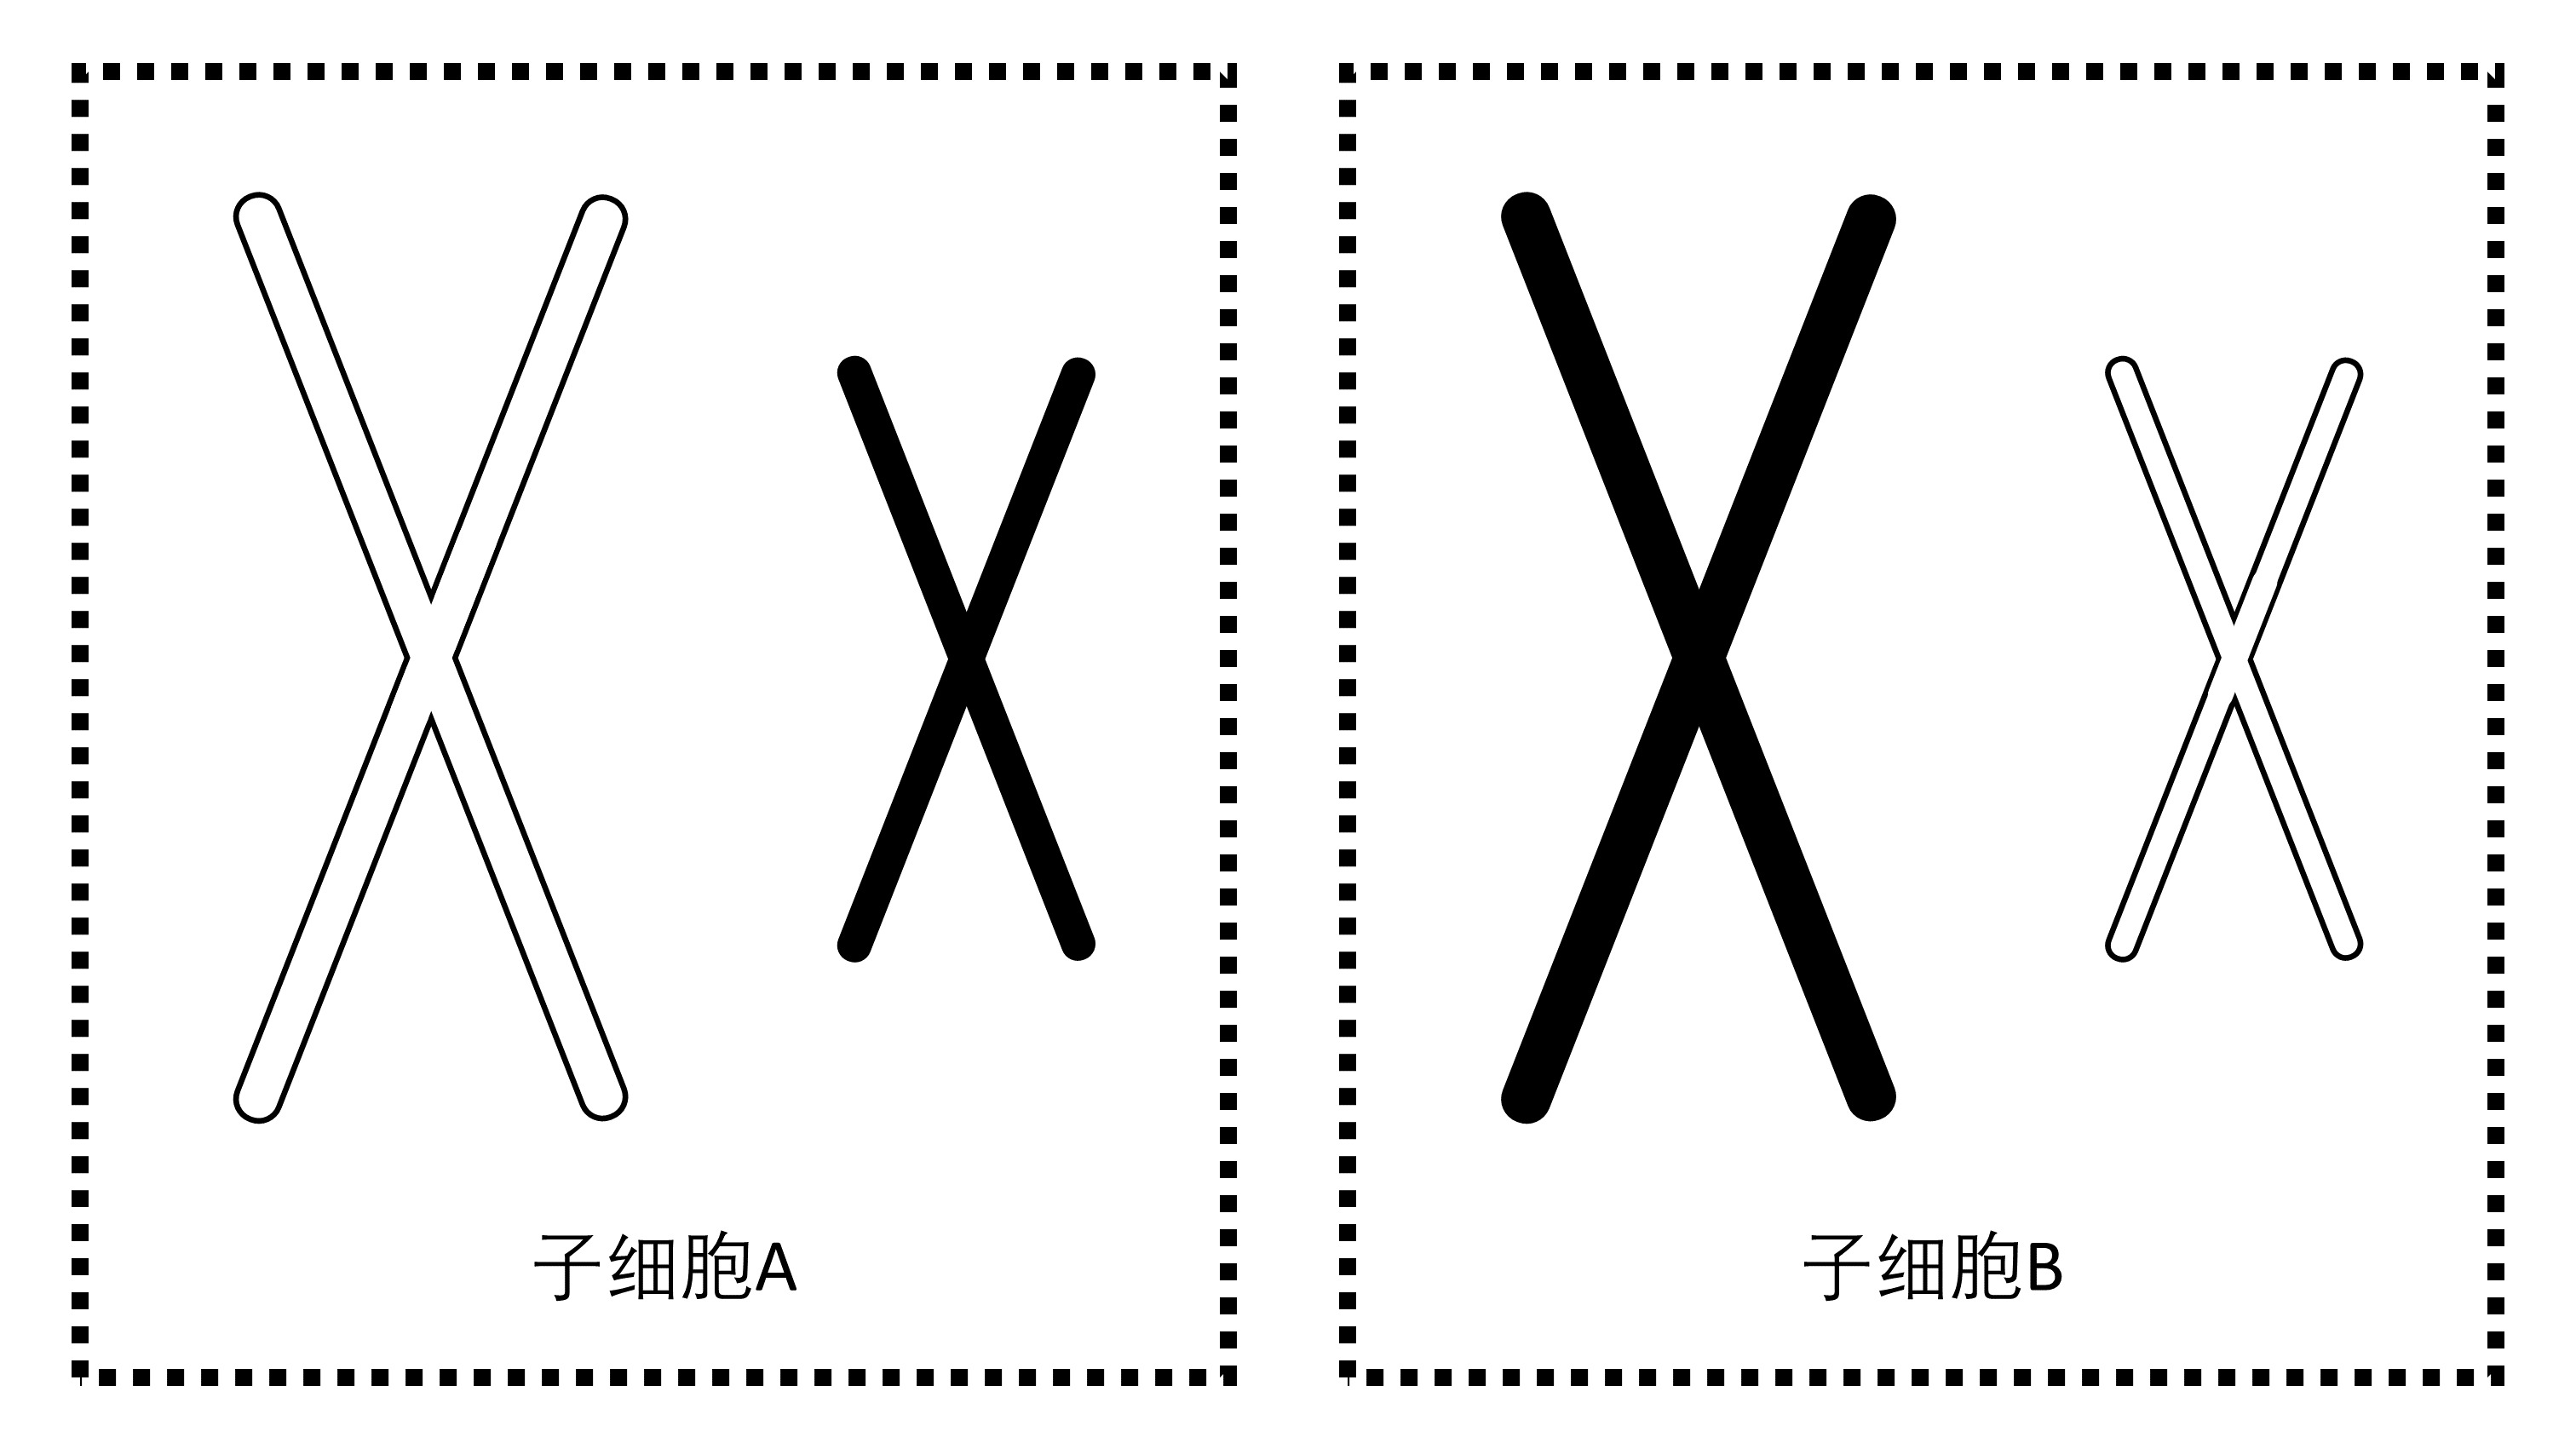
\includegraphics[width=10cm]{BiologyImage/46.jpg}
            \caption{减数第一次分裂后的染色质状况}
        \end{center}
    \end{figure}

\newpage

\subsubsection{减数第二次分裂间期}
    减数第二次分裂间期:该间期时间相对较短,这是由于不需要进行染色体的复制。\\[4mm]
    减数第二次分裂间期:
    \begin{figure}[h]
        \begin{center}
            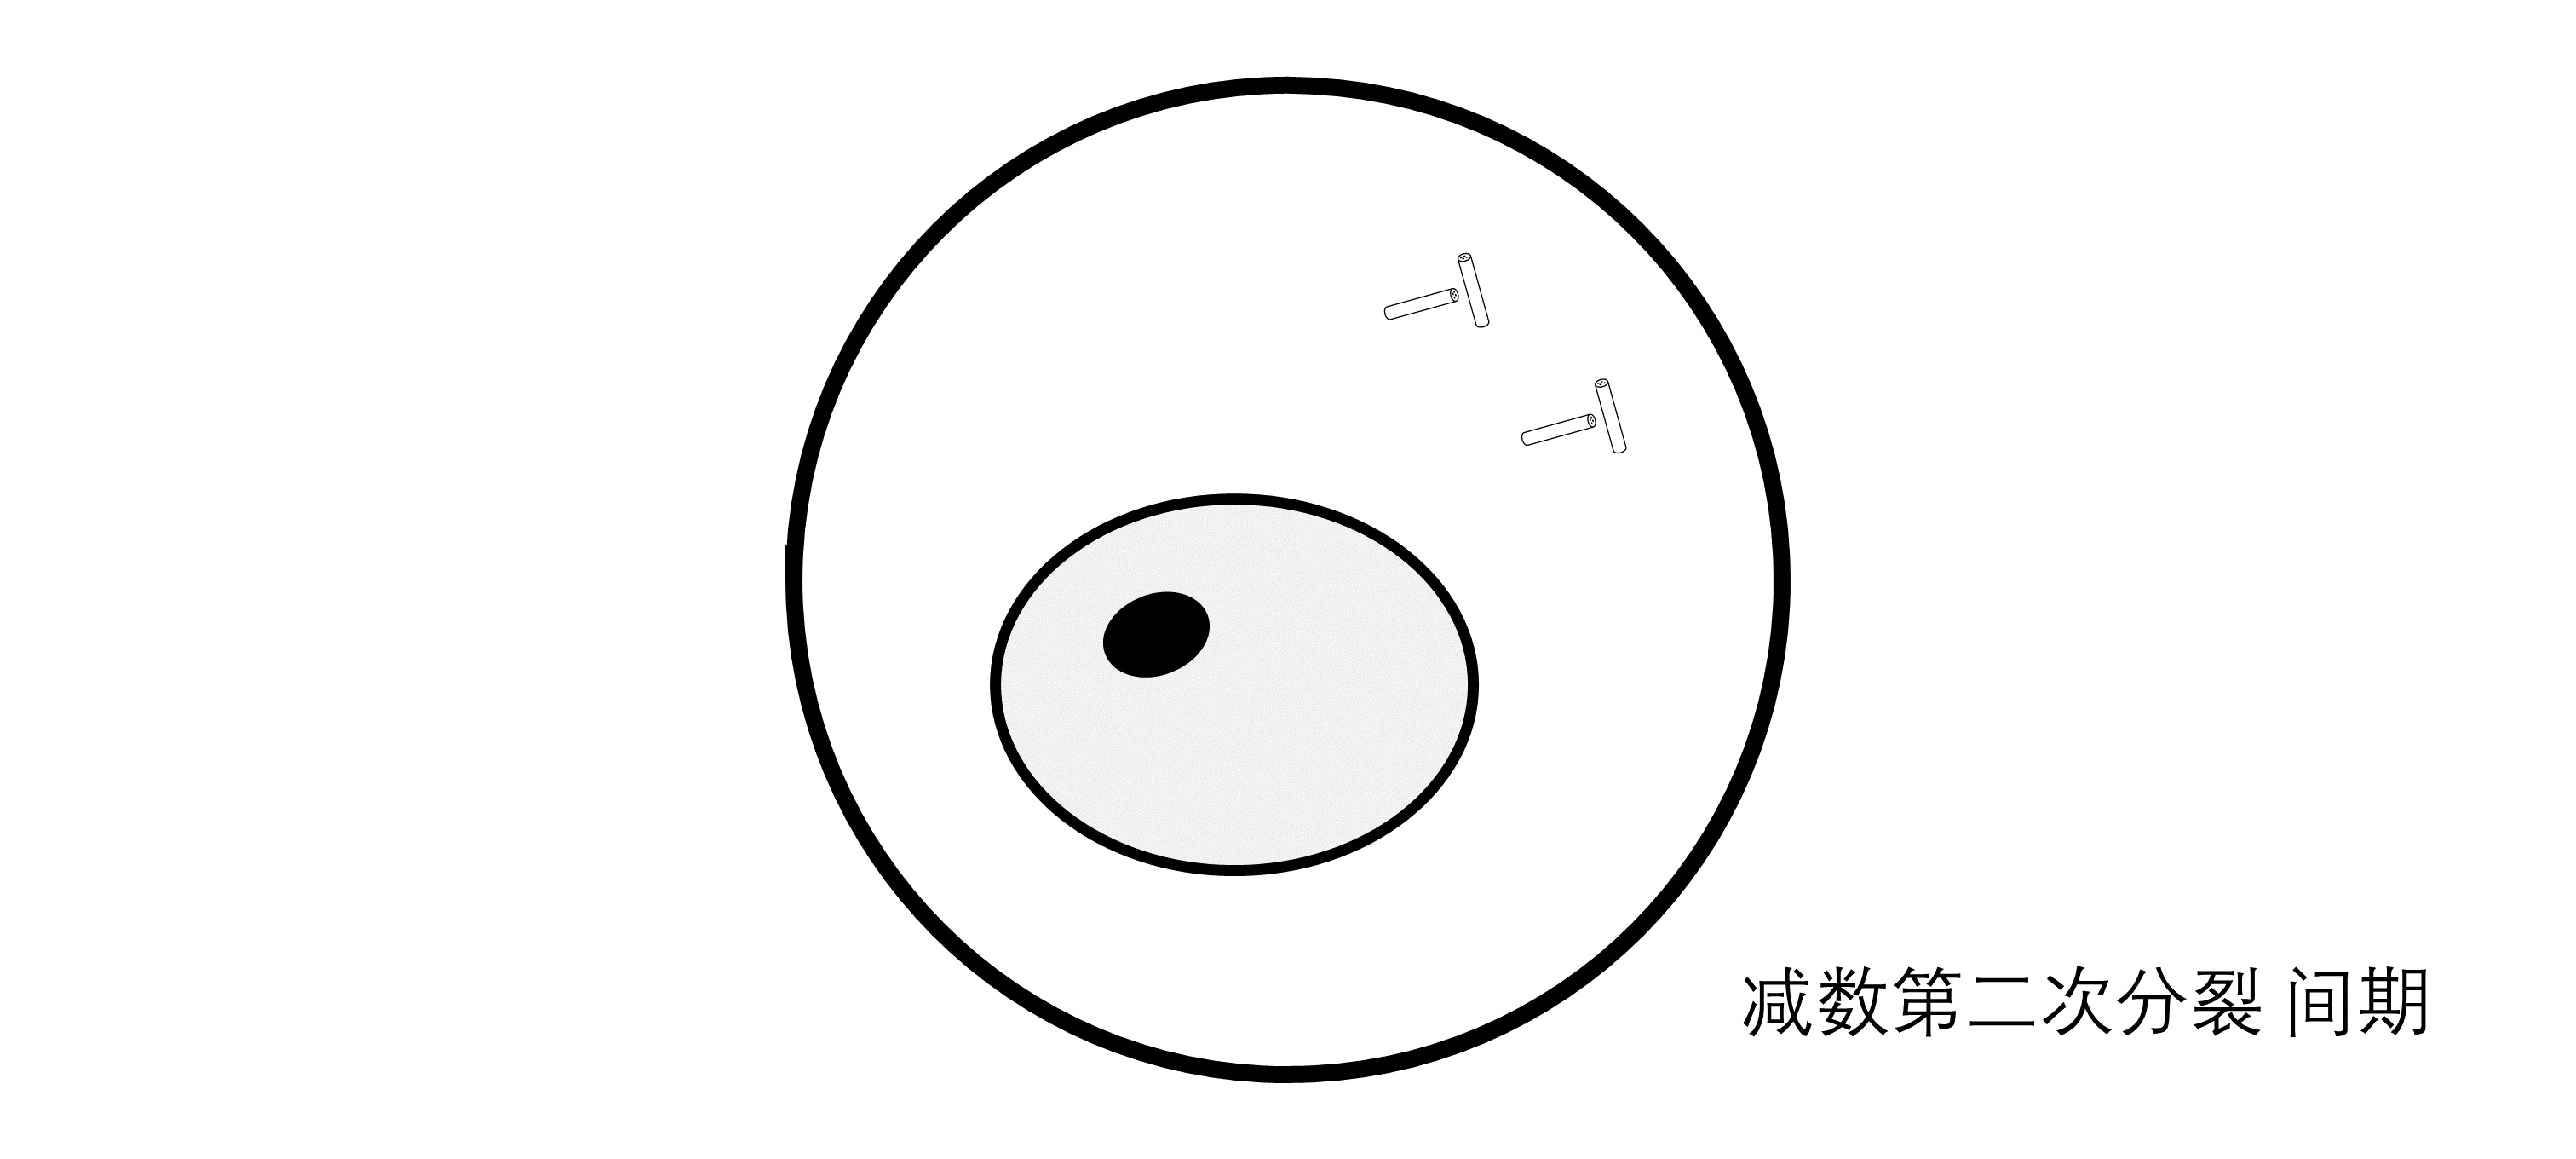
\includegraphics[width=10cm]{BiologyImage/39.jpg}
            \caption{减数第二次分裂间期}
        \end{center}
    \end{figure}

\subsubsection{减数第二次分裂前期}
    减数第二次分裂前期:核仁核膜消失,染色质螺旋缠绕形成染色体,细胞中出现了梭形的纺锤体。\\[4mm]
    减数第二次分裂前期:
    \begin{figure}[h]
        \begin{center}
            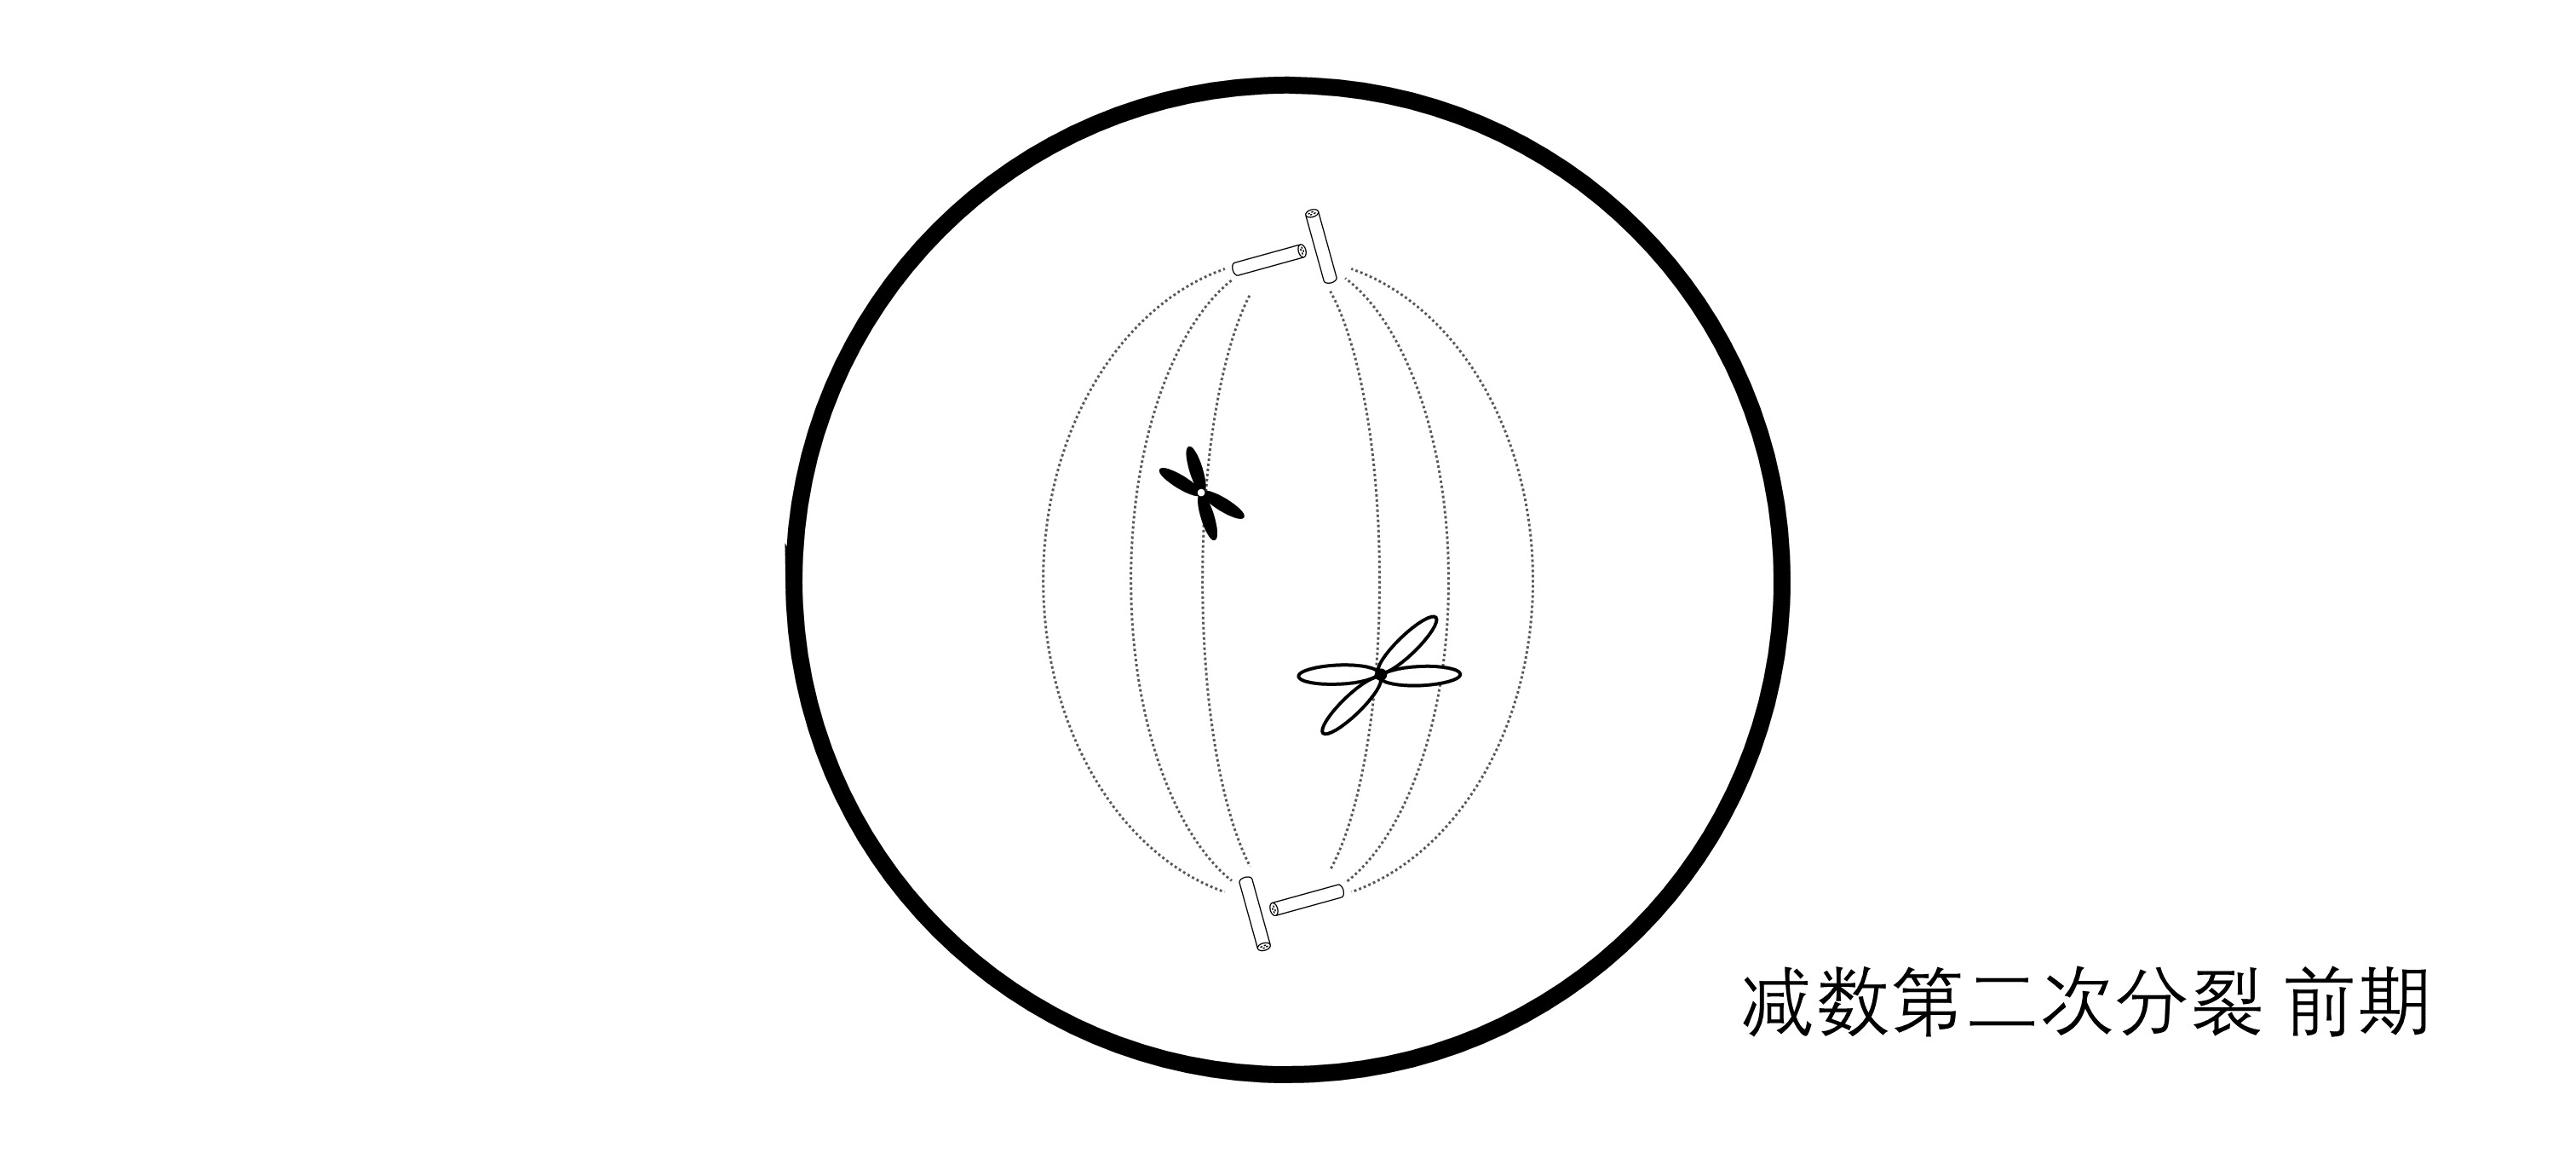
\includegraphics[width=10cm]{BiologyImage/40.jpg}
            \caption{减数第二次分裂前期}
        \end{center}
    \end{figure}

\newpage

\subsubsection{减数第二次分裂中期}
    减数第二次分裂中期:着丝粒与纺锤丝相连,染色体在纺锤丝的牵引下排列赤道面。\\[4mm]
    减数第二次分裂中期:
    \begin{figure}[h]
        \begin{center}
            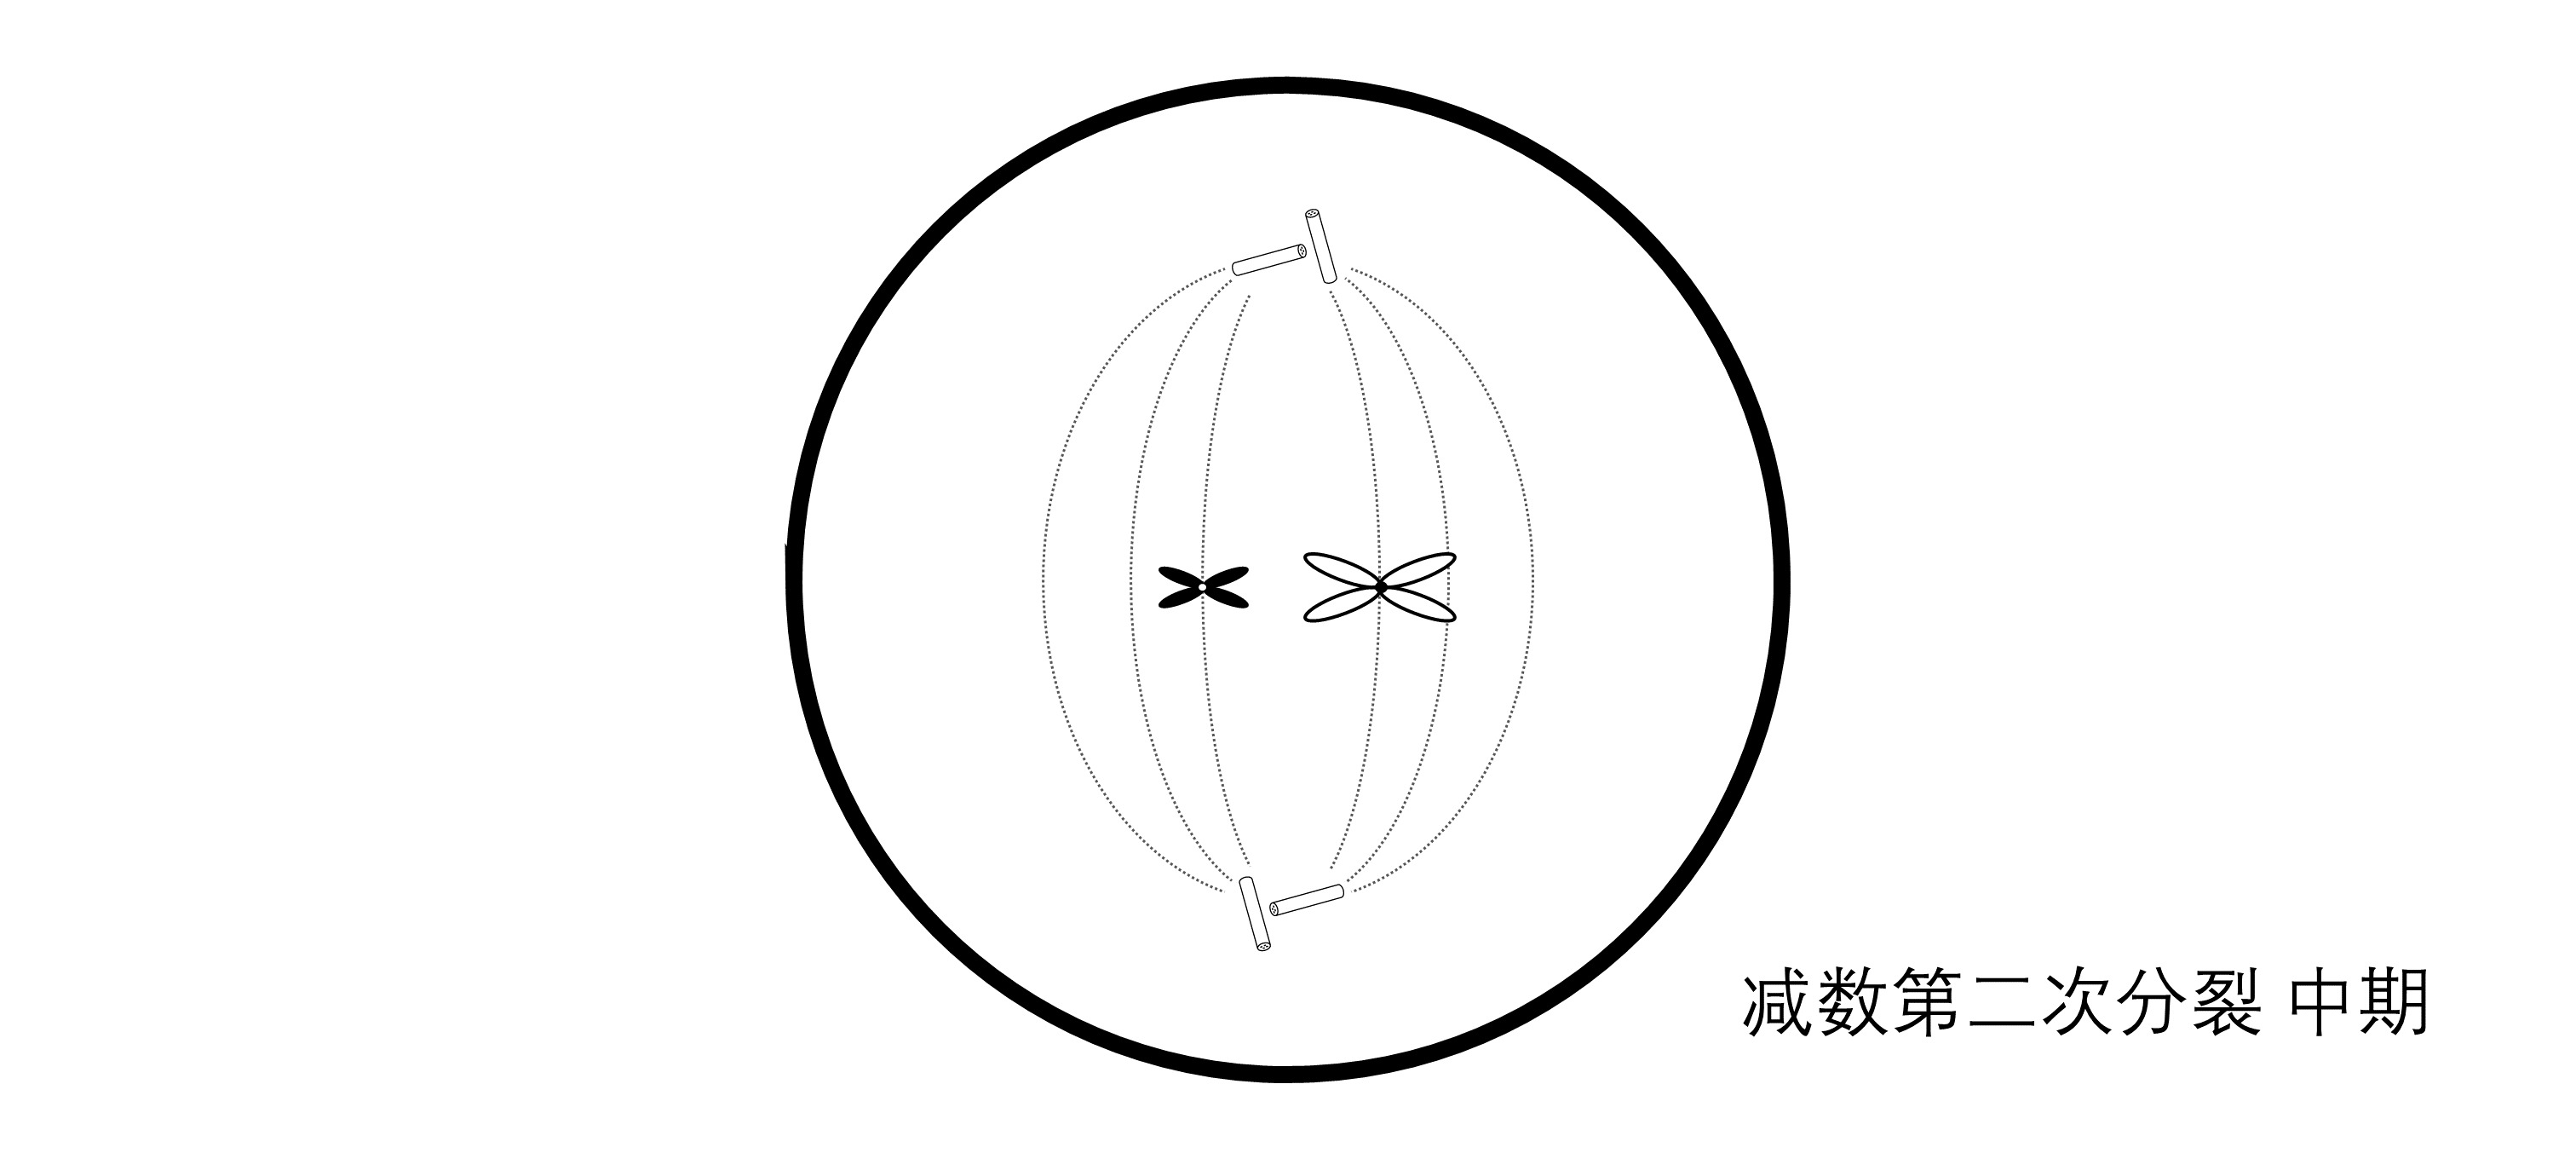
\includegraphics[width=10cm]{BiologyImage/41.jpg}
            \caption{减数第二次分裂中期}
        \end{center}
    \end{figure}

\subsubsection{减数第二次分裂后期}
    减数第二次分裂后期:随着纺锤丝的牵引,染色单体分离,分别移向细胞两级。\\[4mm]
    减数第二次分裂后期:
    \begin{figure}[h]
        \begin{center}
            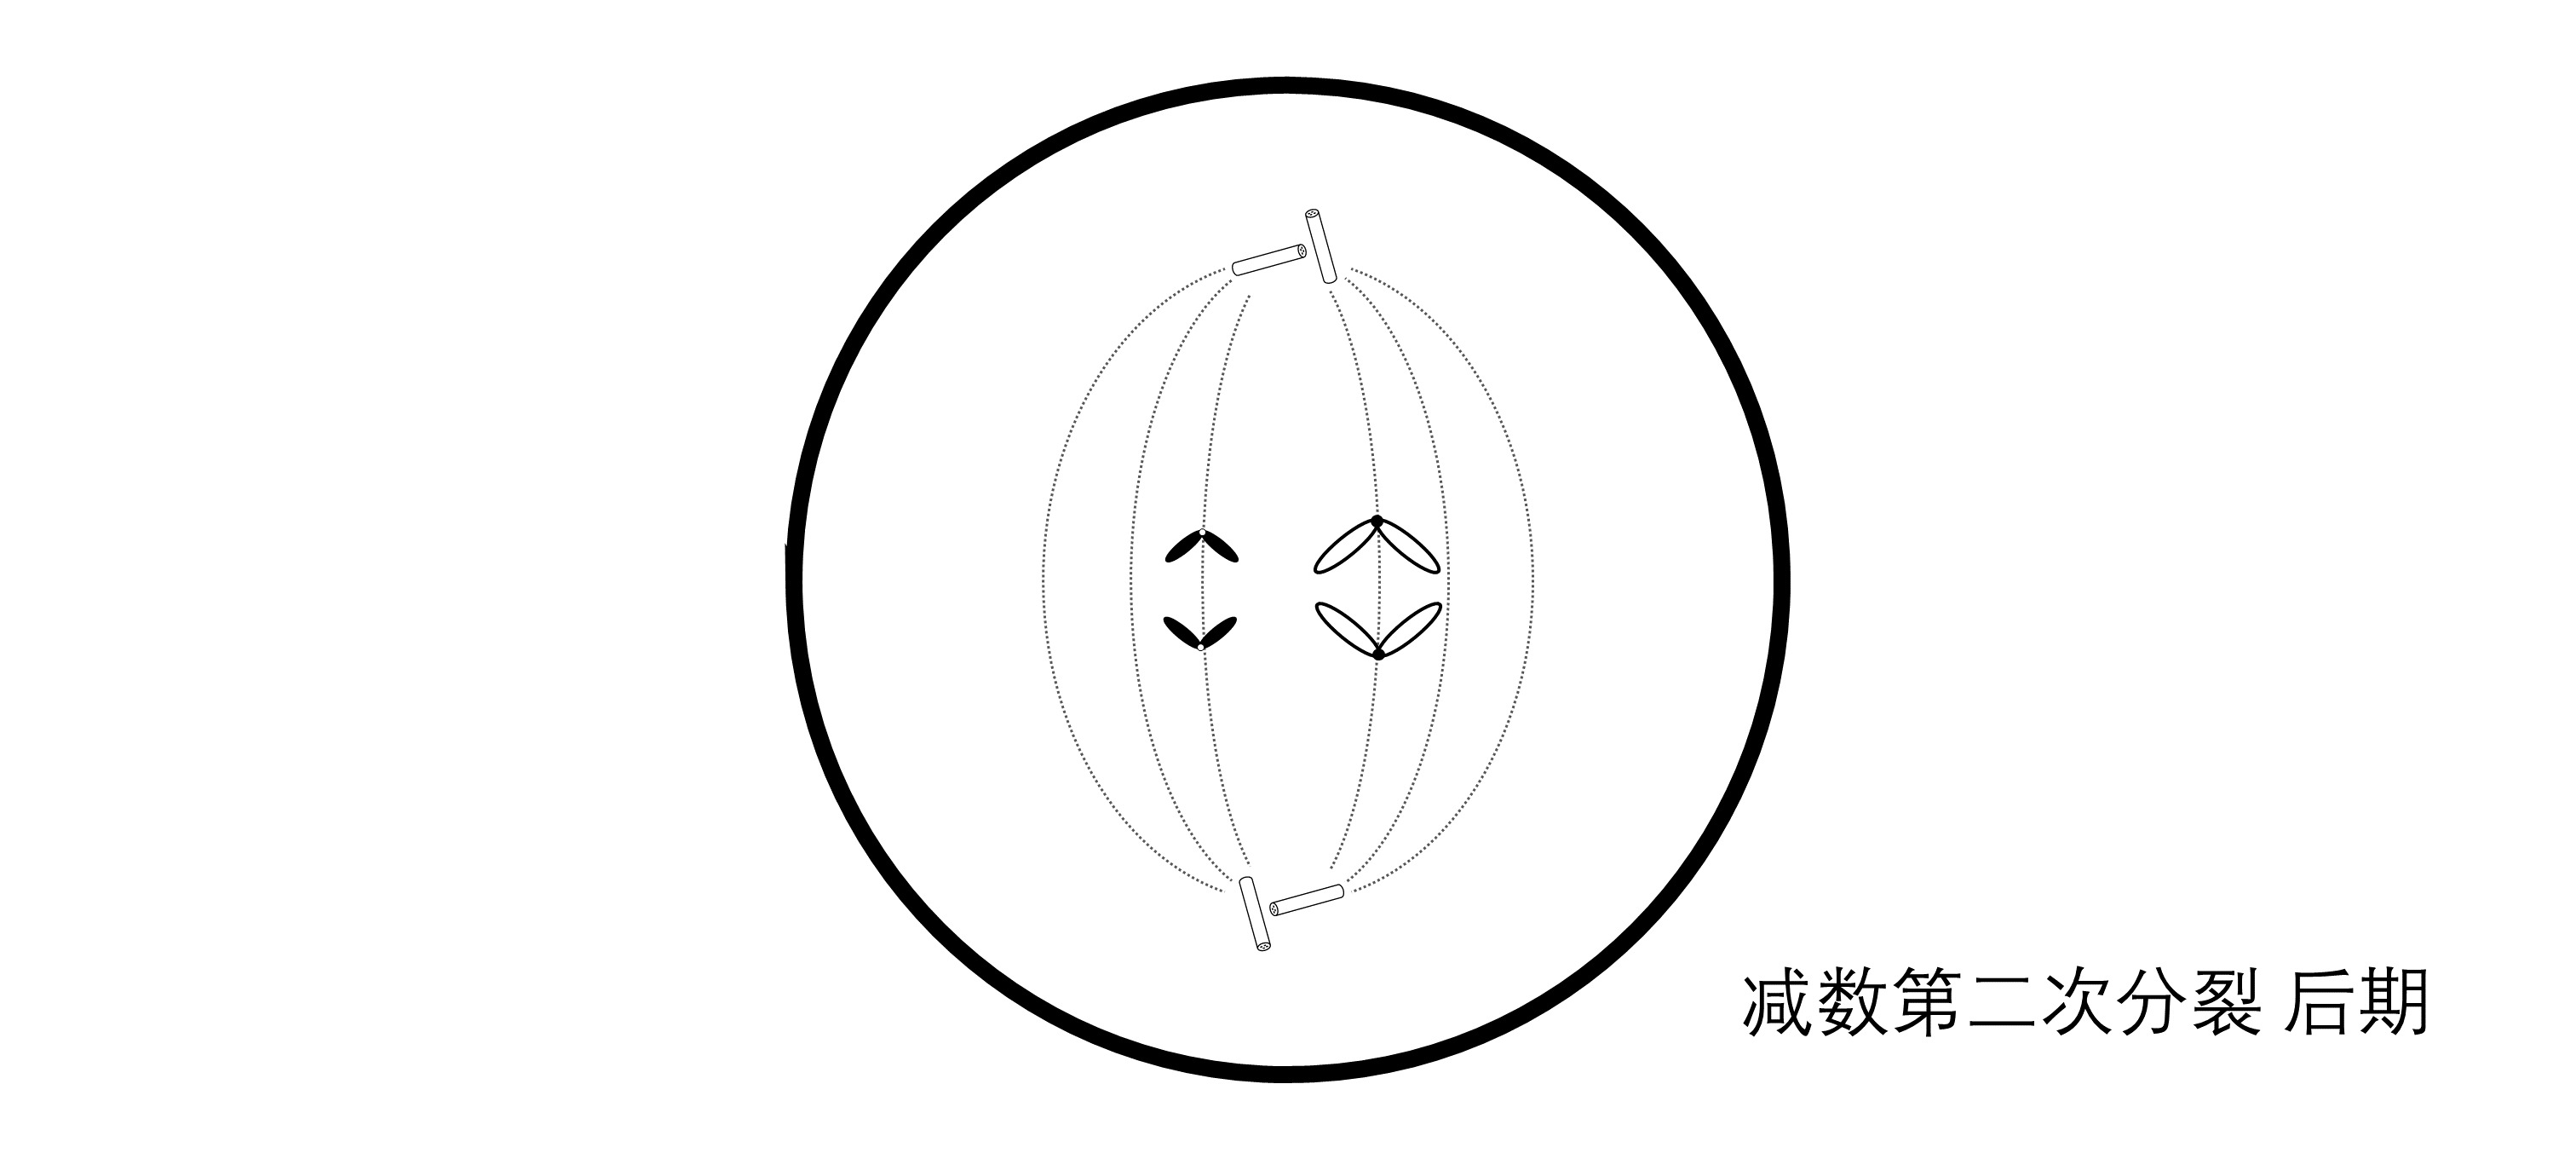
\includegraphics[width=10cm]{BiologyImage/42.jpg}
            \caption{减数第二次分裂后期}
        \end{center}
    \end{figure}

\newpage

\subsubsection{减数第二次分裂末期}
    减数第二次分裂末期:当两组染色体分别移到细胞两级之后,细胞分裂为两个子细胞。\\[4mm]
    减数第二次分裂末期:
    \begin{figure}[h]
        \begin{center}
            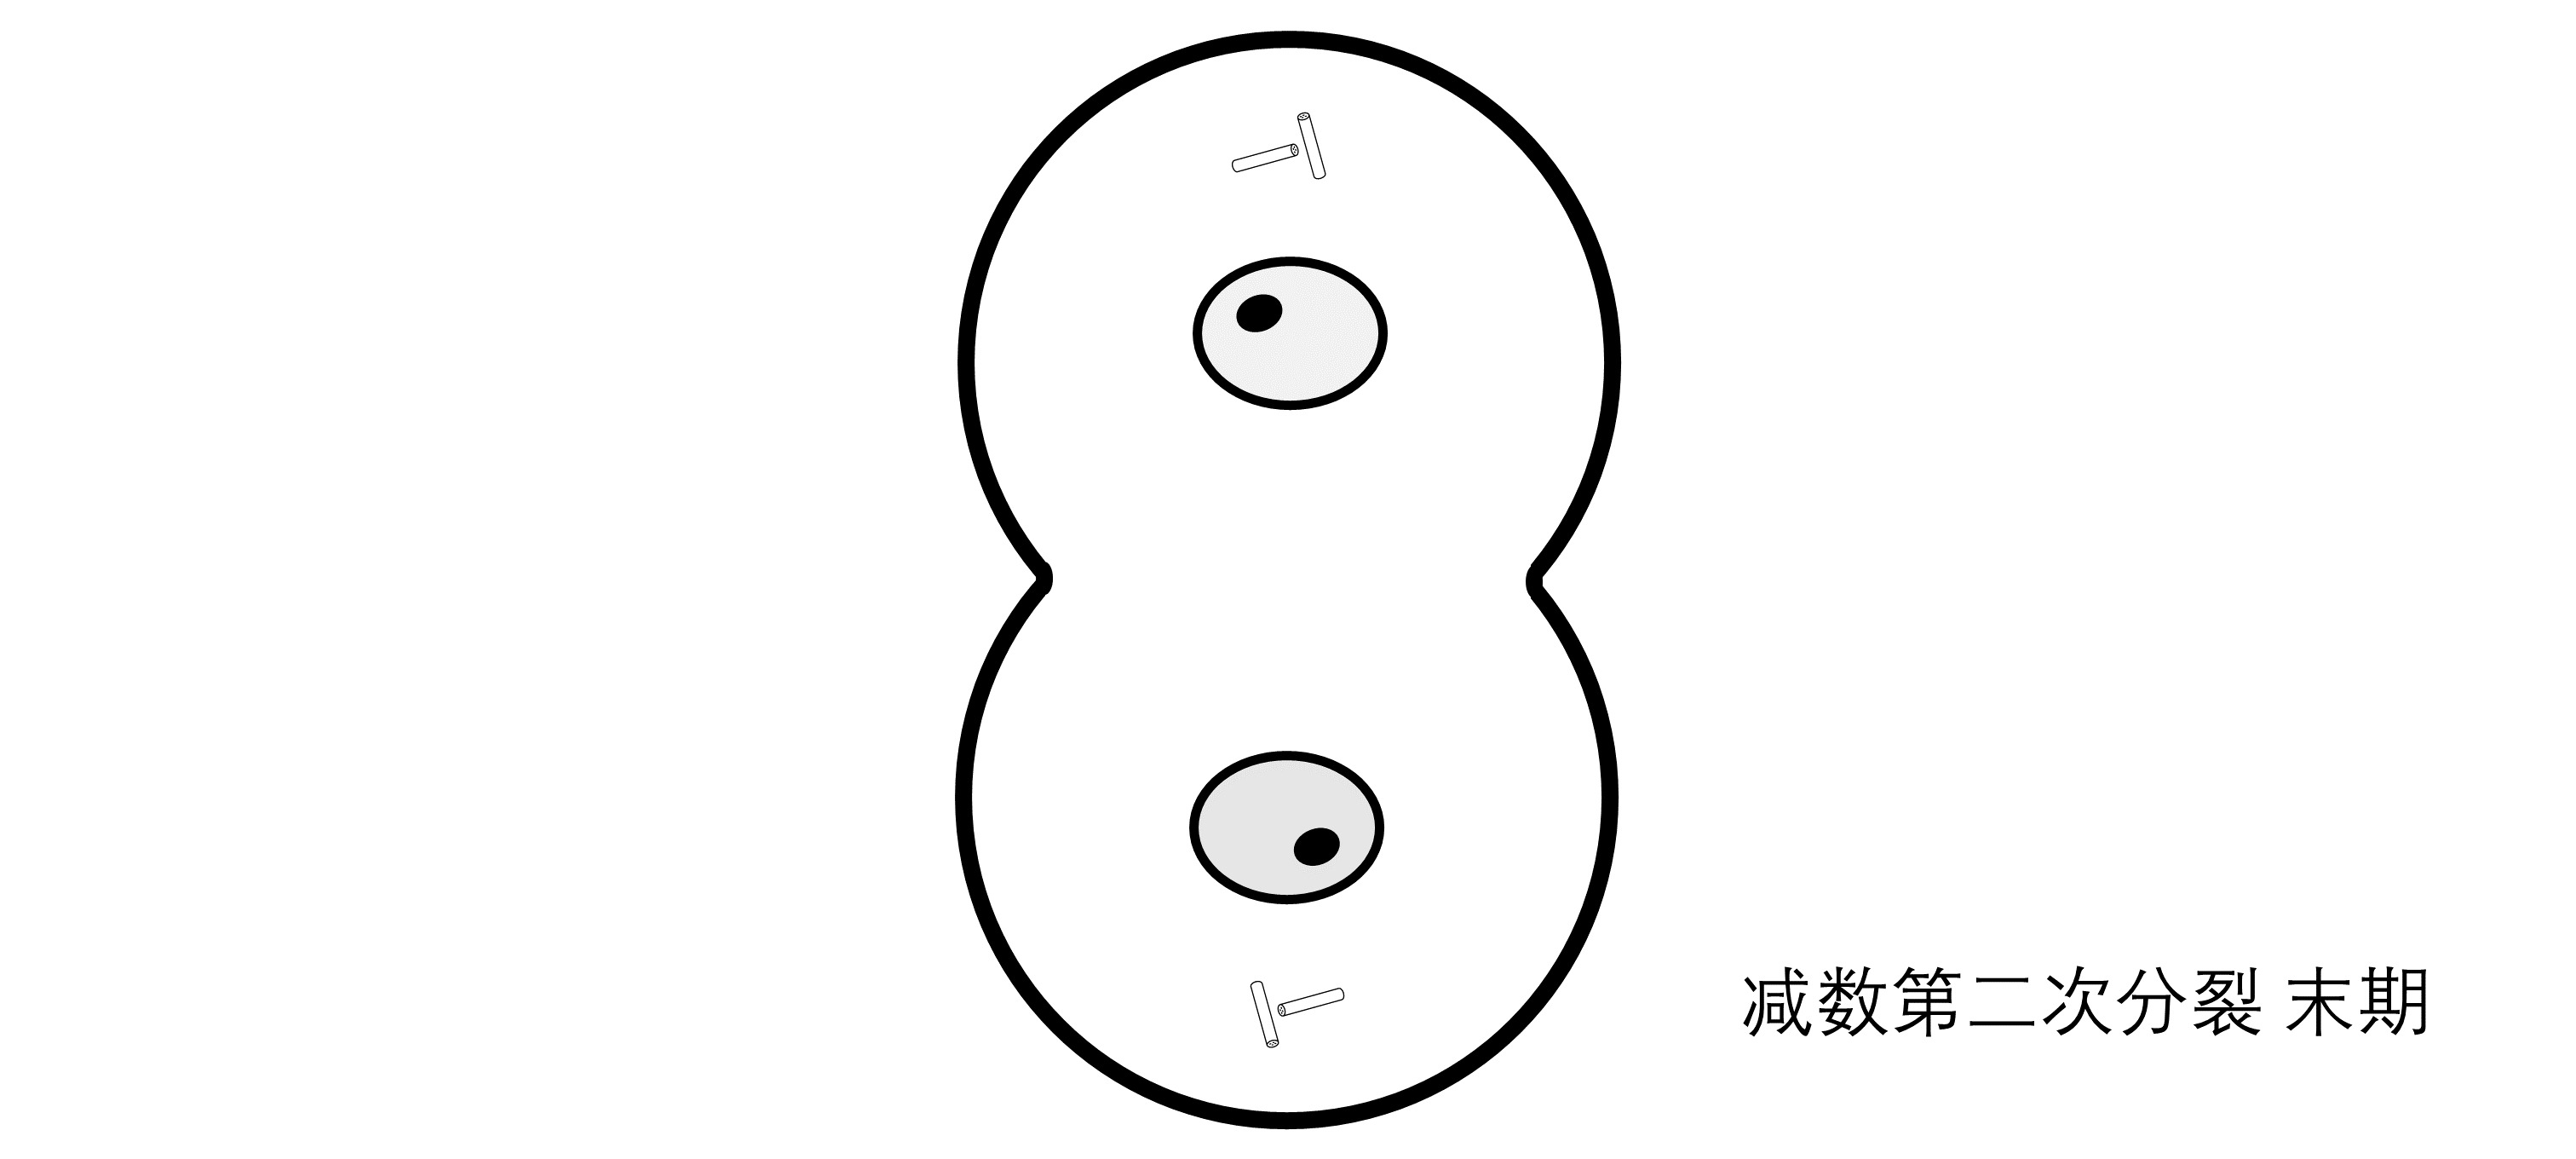
\includegraphics[width=10cm]{BiologyImage/43.jpg}
            \caption{减数第二次分裂末期}
        \end{center}
    \end{figure}\\

\subsubsection{减数第二次分裂后的染色质状况}
    减数第二次分裂后的染色质状况:
    \begin{figure}[h]
        \begin{center}
            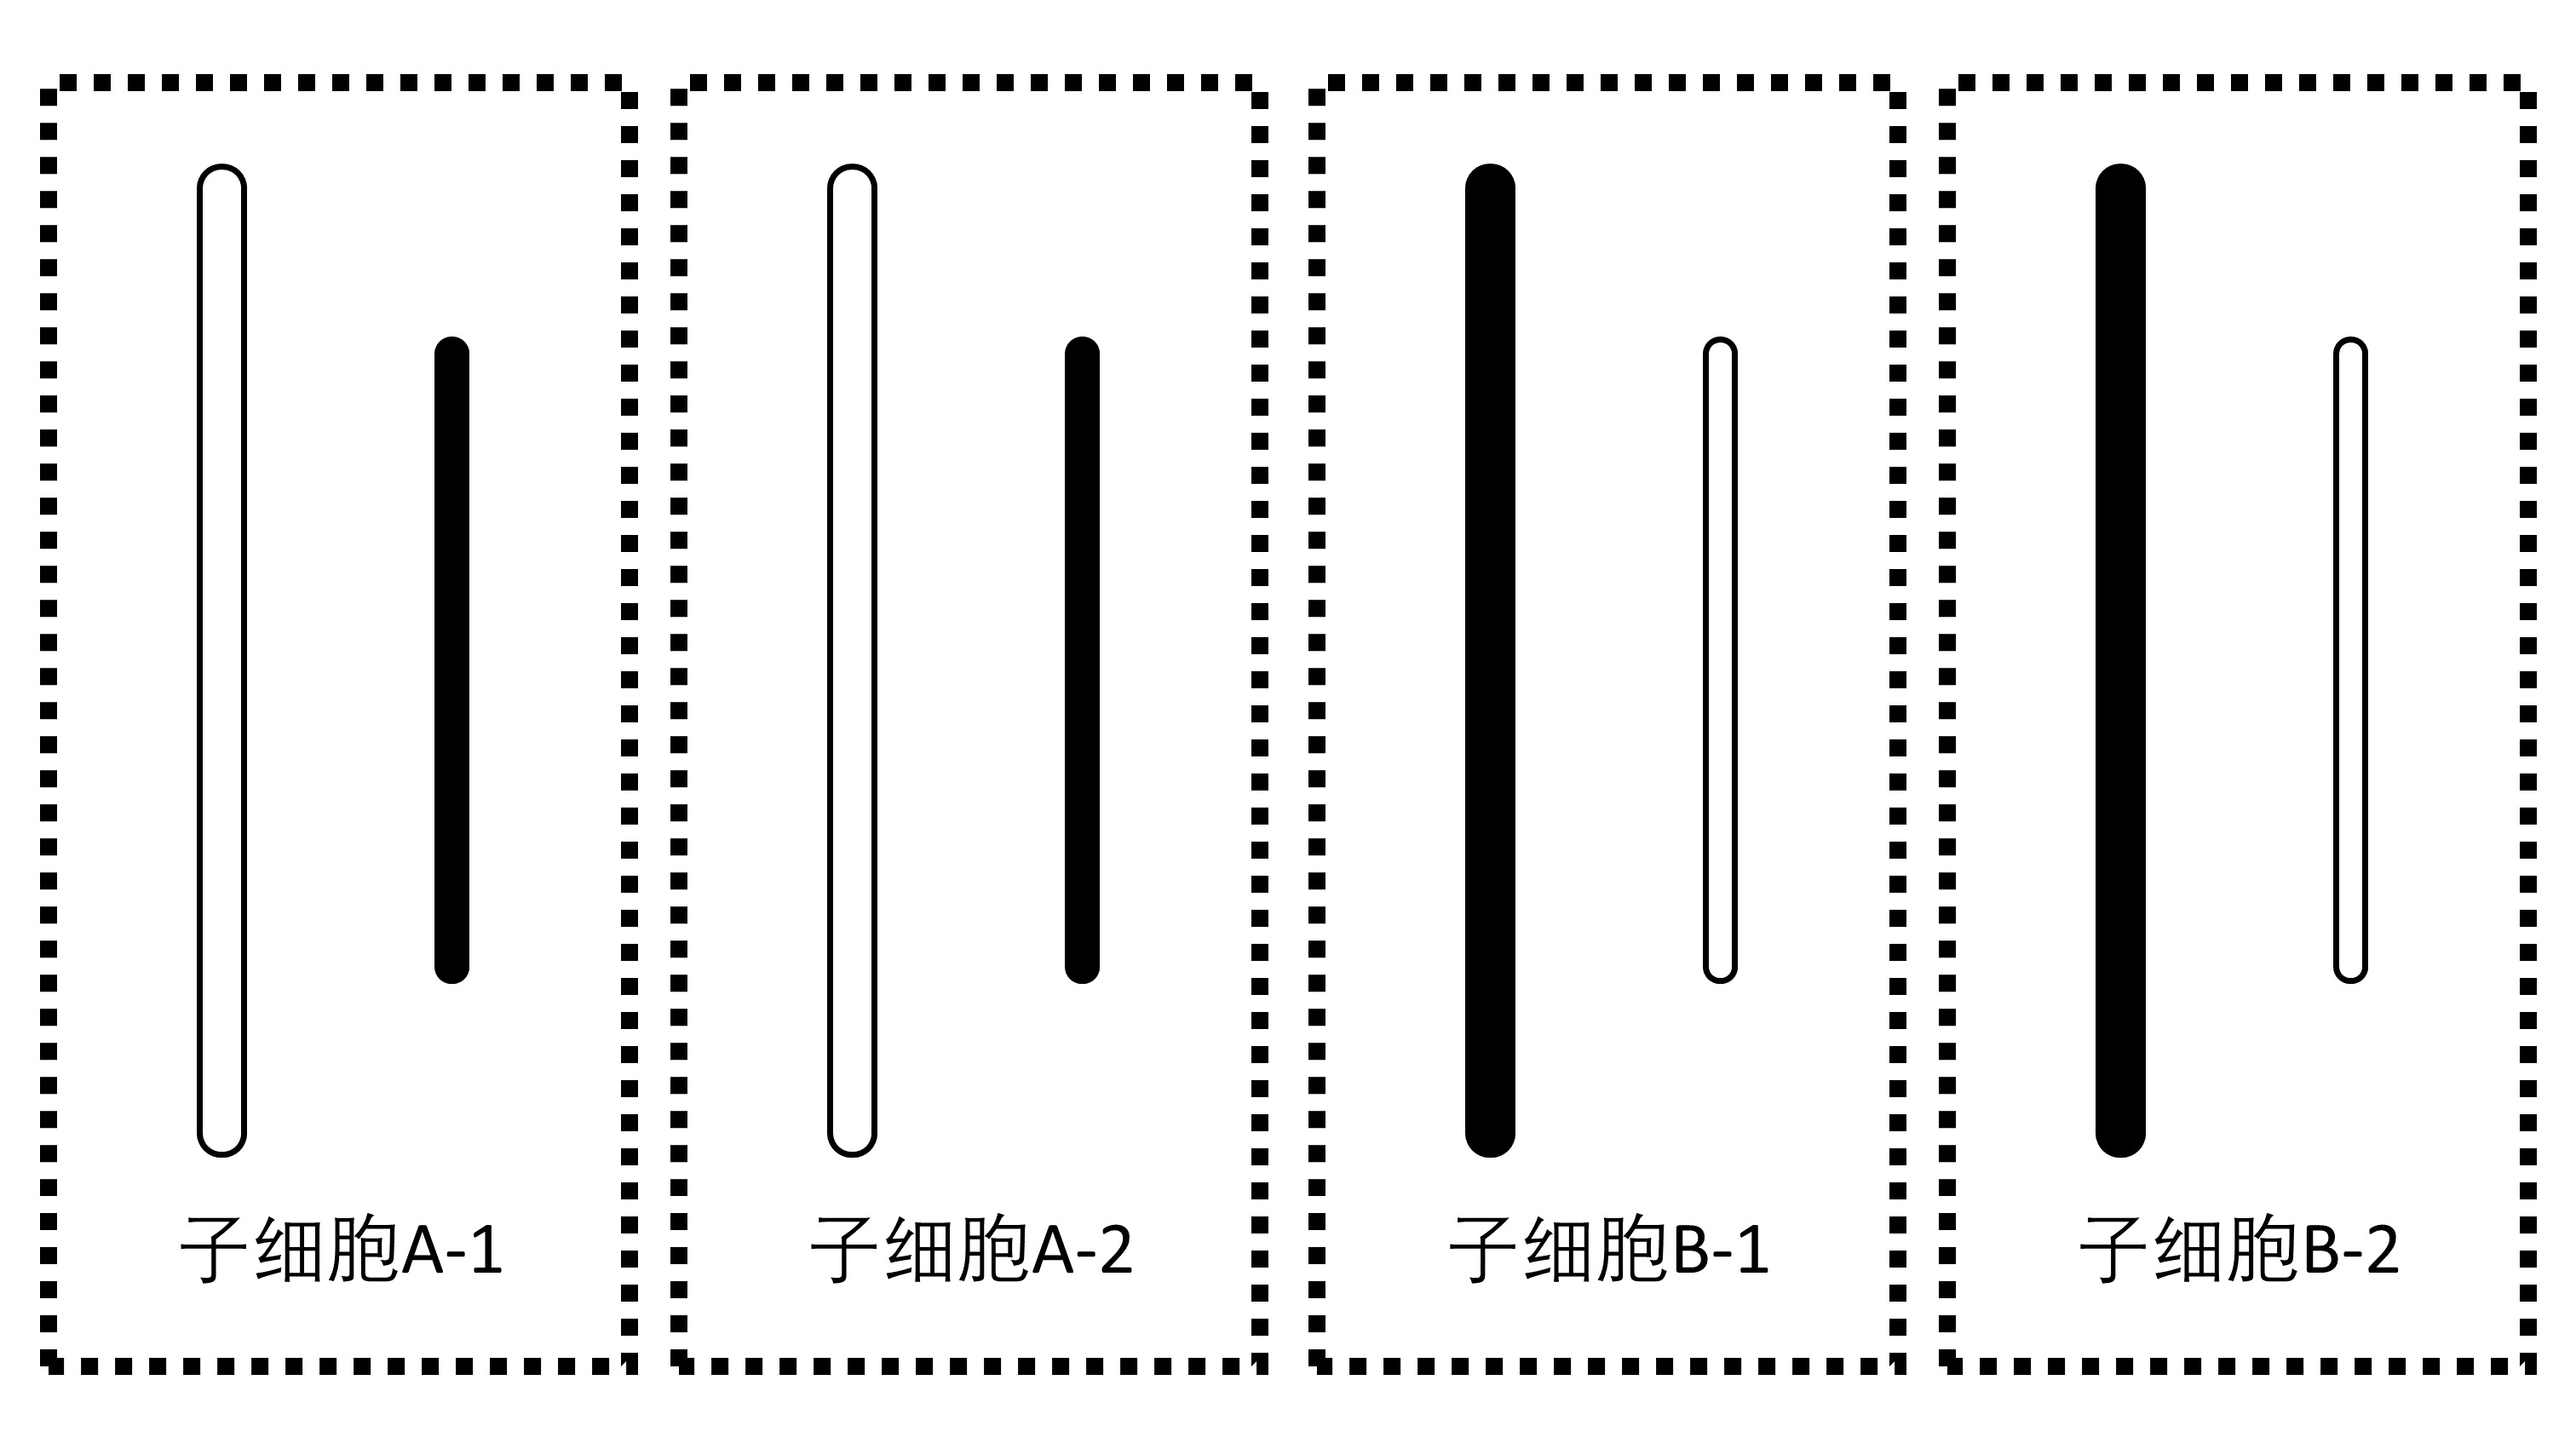
\includegraphics[width=10cm]{BiologyImage/47.jpg}
            \caption{减数第二次分裂后的染色质状况}
        \end{center}
    \end{figure}

\newpage

\subsection{精子和卵子的形成}
    精子的形成由睾丸中的精原细胞开始:
    \begin{figure}[h]
        \begin{center}
            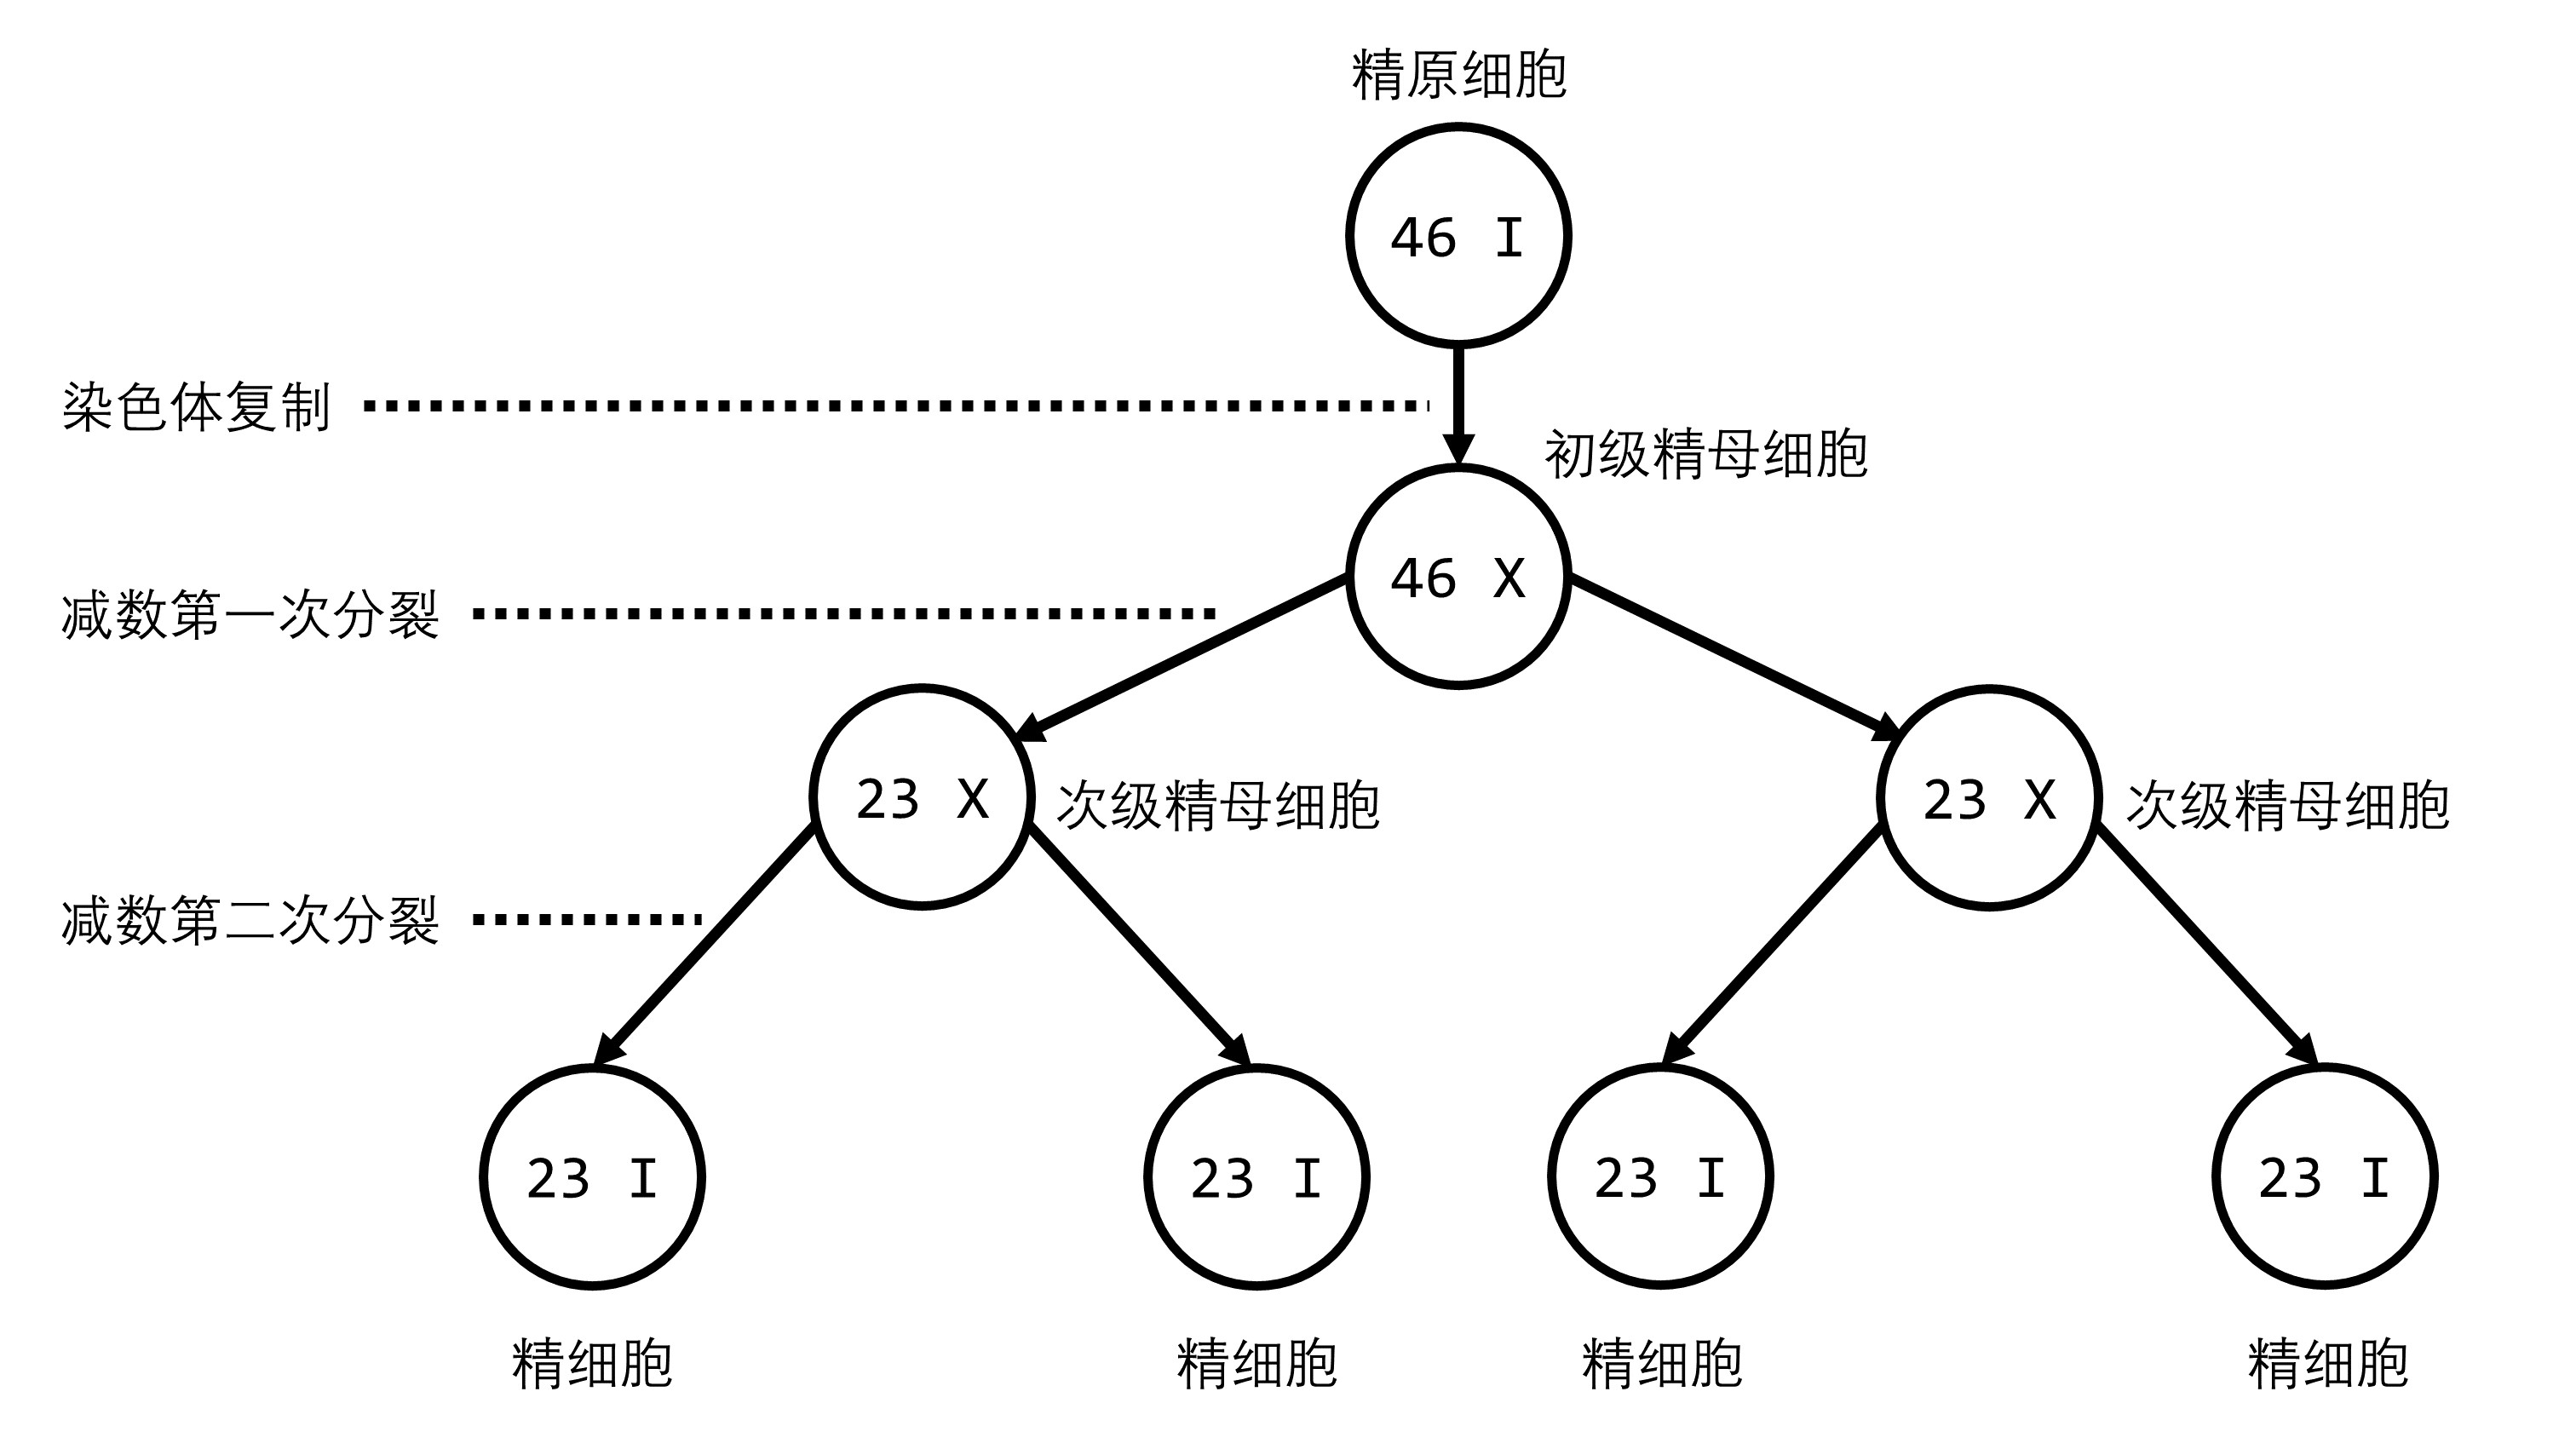
\includegraphics[width=10cm]{BiologyImage/48.jpg}
            \caption{精子的形成}
        \end{center}
    \end{figure}\\
    卵子的形成由卵巢中的精原细胞开始:
    \begin{figure}[h]
        \begin{center}
            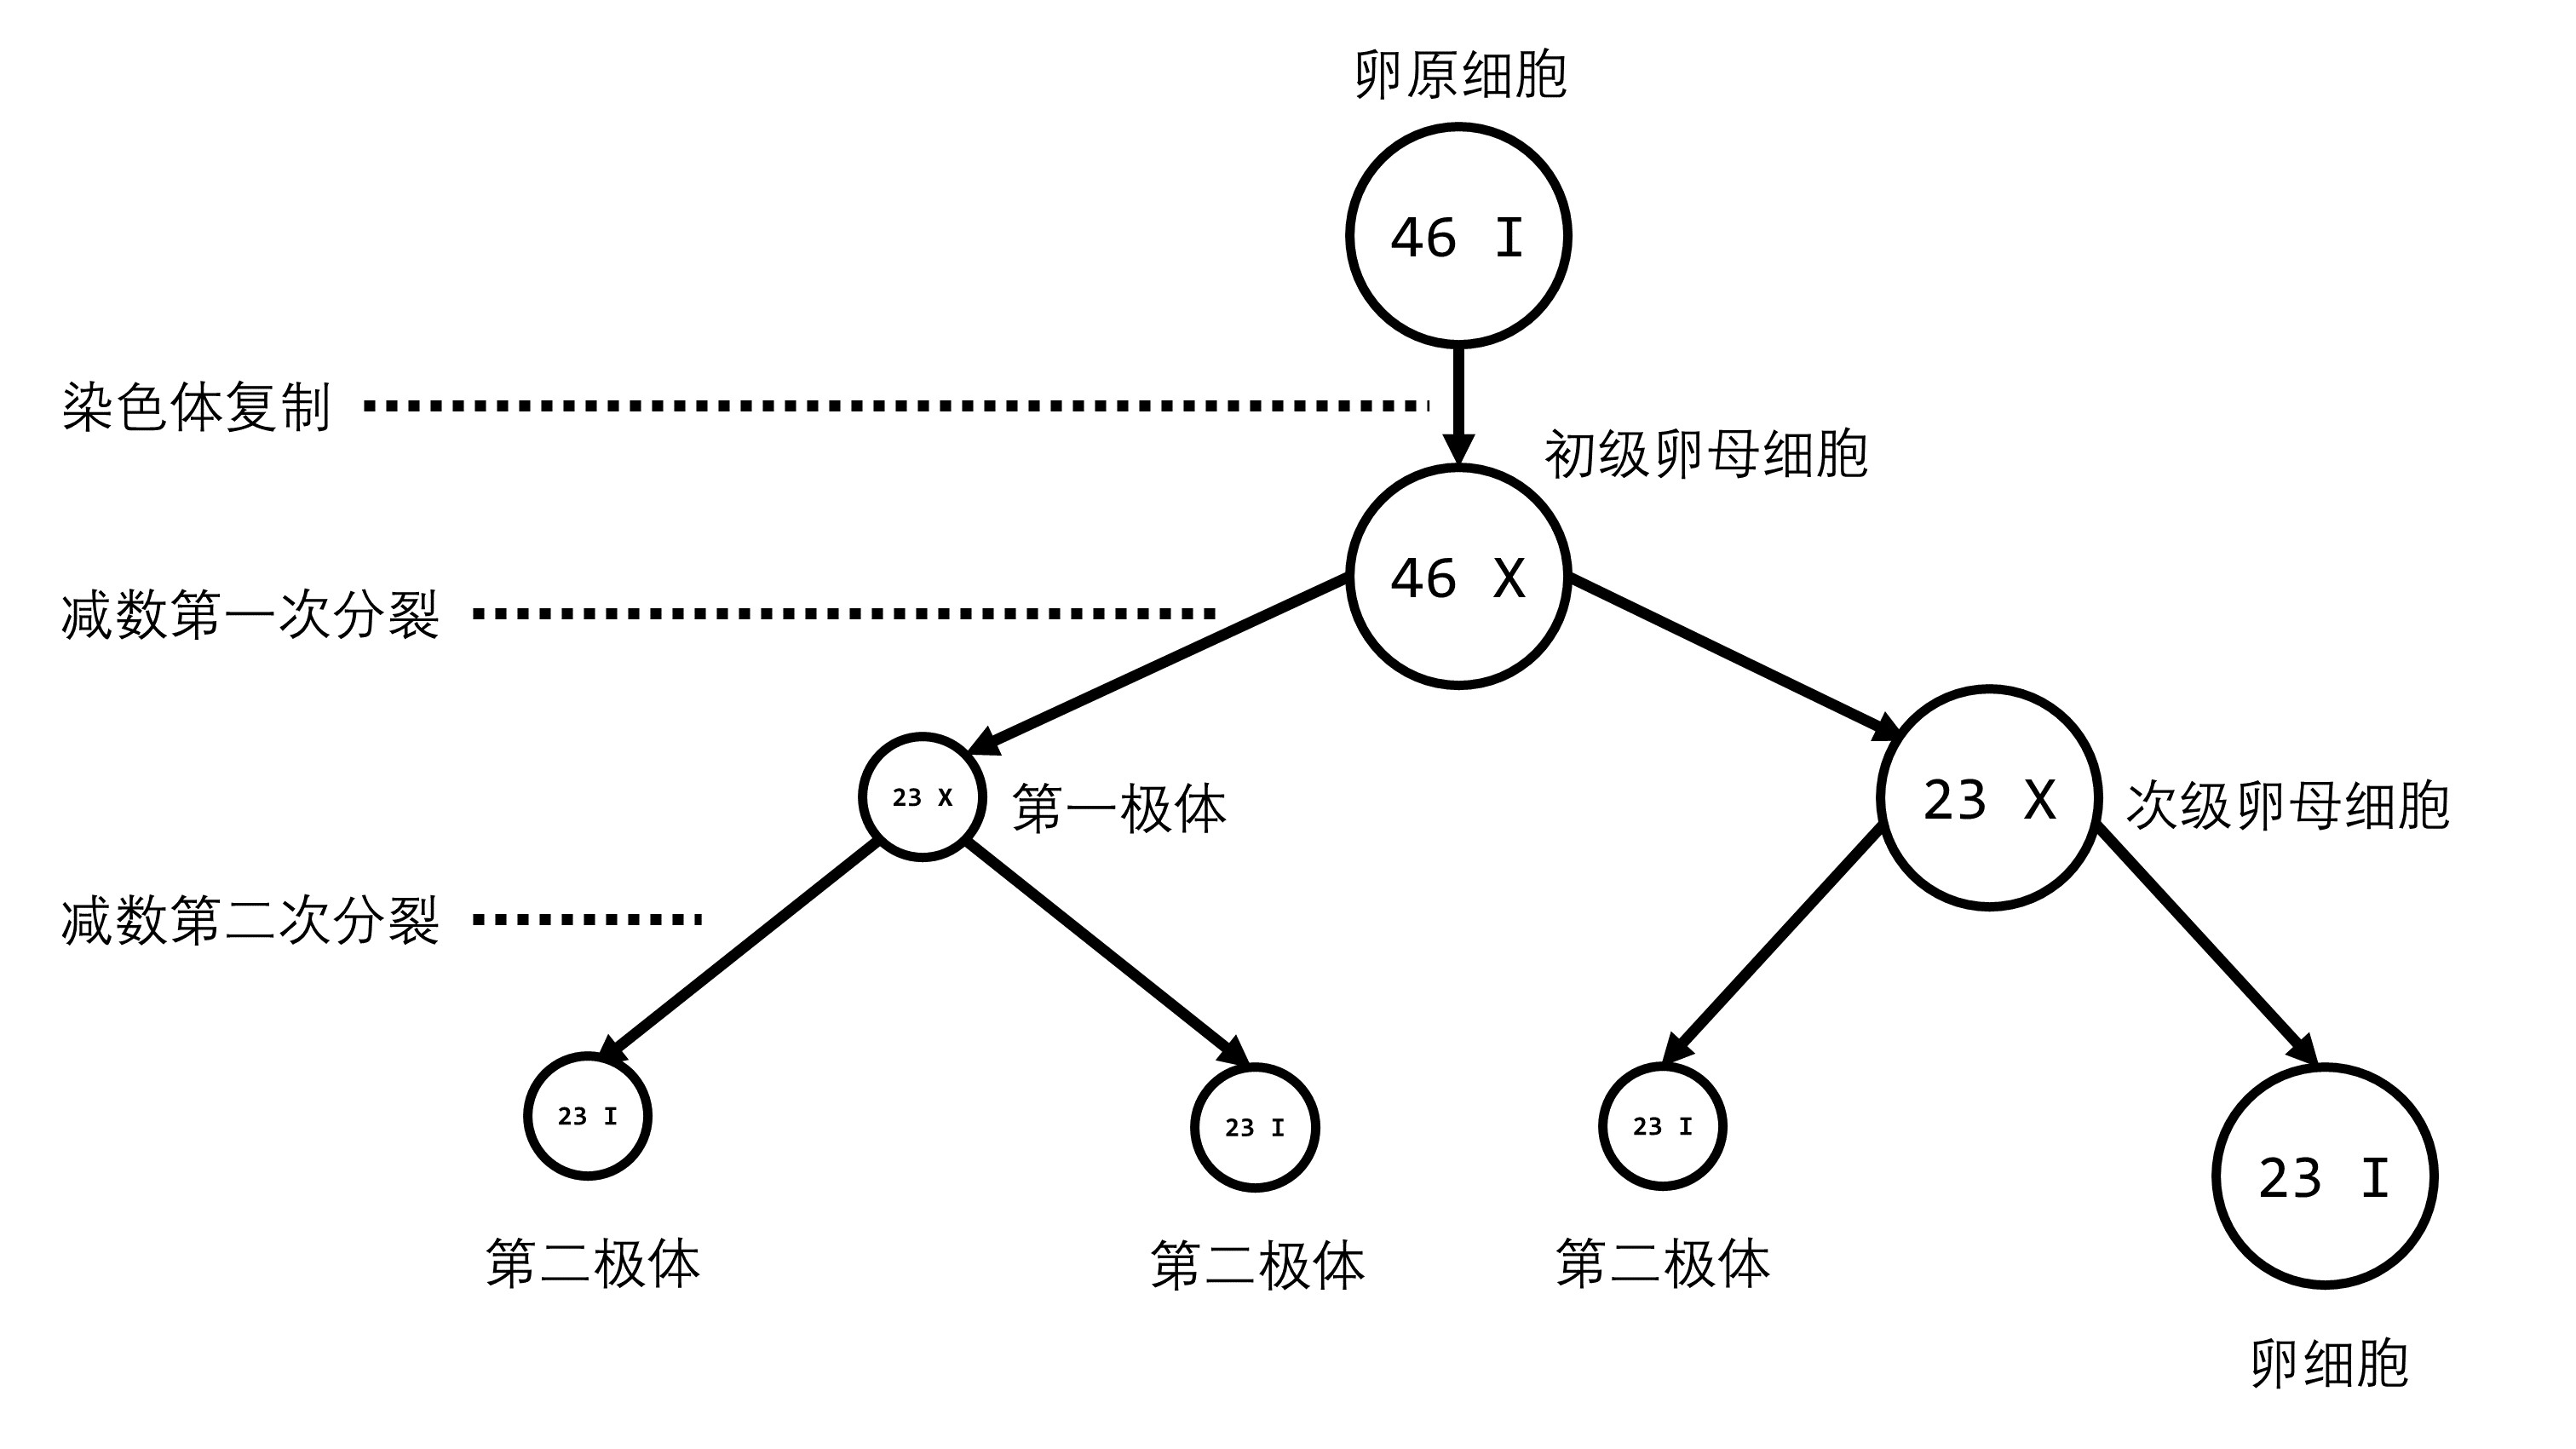
\includegraphics[width=10cm]{BiologyImage/49.jpg}
            \caption{卵子的形成}
        \end{center}
    \end{figure} \\
    需要说明的是,精细胞还需要通过变形才能成为精子,卵细胞实际上就是卵子。\\[3mm]
    需要指出的是,卵子形成过程中存在不均等分裂,这是为了使得卵子中包含尽可能多的细胞质,
    从而保证受精卵在早期有足够的营养进行发育。副产物第一极体和第二极体均会自行退化消失。

\newpage

\section{微生物}

\subsection{微生物的分类}
    生物可以首先分为以下三类:
    \vspace{5pt}
    \begin{table}[h]
        \begin{center}
            \begin{tabular}{l|l}
                \hline
                无细胞结构&病毒\\ \hline
                有细胞结构~~无成形细胞核&原核生物\\ \hline
                有细胞结构~~有成形细胞核\qquad\qquad&真核生物\qquad\qquad\\ \hline
            \end{tabular}
            \caption{生物分类}
        \end{center}
    \end{table}\\
    其中真核生物还可以进一步分为:真菌,植物,动物。\\[3mm]
    微生物是生物中肉眼看不见的微小生物的总称。\\[3mm]
    微生物具有以下五个特征:\\[3mm]
    1.个体微小\\[3mm]
    2.结构简单\\[3mm]
    3.分布广泛\\[3mm]
    4.营养方式多样\\[3mm]
    5.生长繁殖快\\

\subsection{消毒和灭菌}
    下表列出了消毒和灭菌的差异:\vspace{5pt}
    \begin{table}[h]
        \begin{center}
            \begin{tabular}{l|l|l|l|l}
                \hline
                消毒\qquad\qquad&巴氏消毒法\qquad\qquad&62$^\circ$C\qquad\qquad&30min\qquad\qquad&1.00$kg/cm^2$\qquad\qquad\\ \hline
                灭菌\qquad\qquad&高压蒸汽灭菌法\qquad\qquad&121$^\circ$C\qquad\qquad&30min\qquad\qquad&1.05$kg/cm^2$\qquad\qquad\\ \hline
            \end{tabular}
            \caption{消毒和灭菌的差异}
        \end{center}
    \end{table}\\
    以细菌为例,消毒只能逼迫细菌进入休眠状态,形成芽孢,而灭菌则可以彻底杀死芽孢。\\[3mm]
    使用巴氏消毒法的牛奶必须冷藏保存,由于消毒过程中温度较低,风味较好。\\[3mm]
    使用高压蒸汽灭菌法的牛奶可以常温保存,由于消灭菌过程中温度较高,风味较差。\\[6mm]
    巴氏消毒法由法国微生物学家巴斯德提出。

\newpage

\subsection{病毒}
    病毒是一类没有细胞结构的生物。\\[6mm]
    病毒由衣壳和核心组成:\\[3mm]
    衣壳的化学本质是蛋白质,处于病毒外部,起到保护病毒的作用。\\[3mm]
    核心的化学本质是核酸,处于病毒内部,起到存储病毒的遗传信息的作用。\\[6mm]
    某些病毒外侧还有一层包膜,具有包膜的病毒称为包膜病毒,不具有包膜的病毒称为裸露病毒。\\[3mm]
    包膜附着有包膜子粒,包膜的化学本质是脂质,包膜子粒的化学本质是糖蛋白。\\[6mm]
    下表列出了病毒的分类:\vspace{3pt}
    \begin{table}[h]
        \begin{center}
            \begin{tabular}{l|l|l}
                \hline
                病毒类型\qquad\qquad&遗传物质\qquad\qquad&遗传物质合成方式\qquad\qquad\\ \hline
                DNA病毒&DNA&DNA复制\\ \hline
                RNA病毒&RNA&RNA复制\\ \hline
                逆转录病毒&RNA&RNA逆转录\\ \hline
            \end{tabular}
            \caption{病毒的分类}
        \end{center}
    \end{table}\\
    下图展示了病毒的结构:
    \begin{figure}[h]
        \begin{center}
            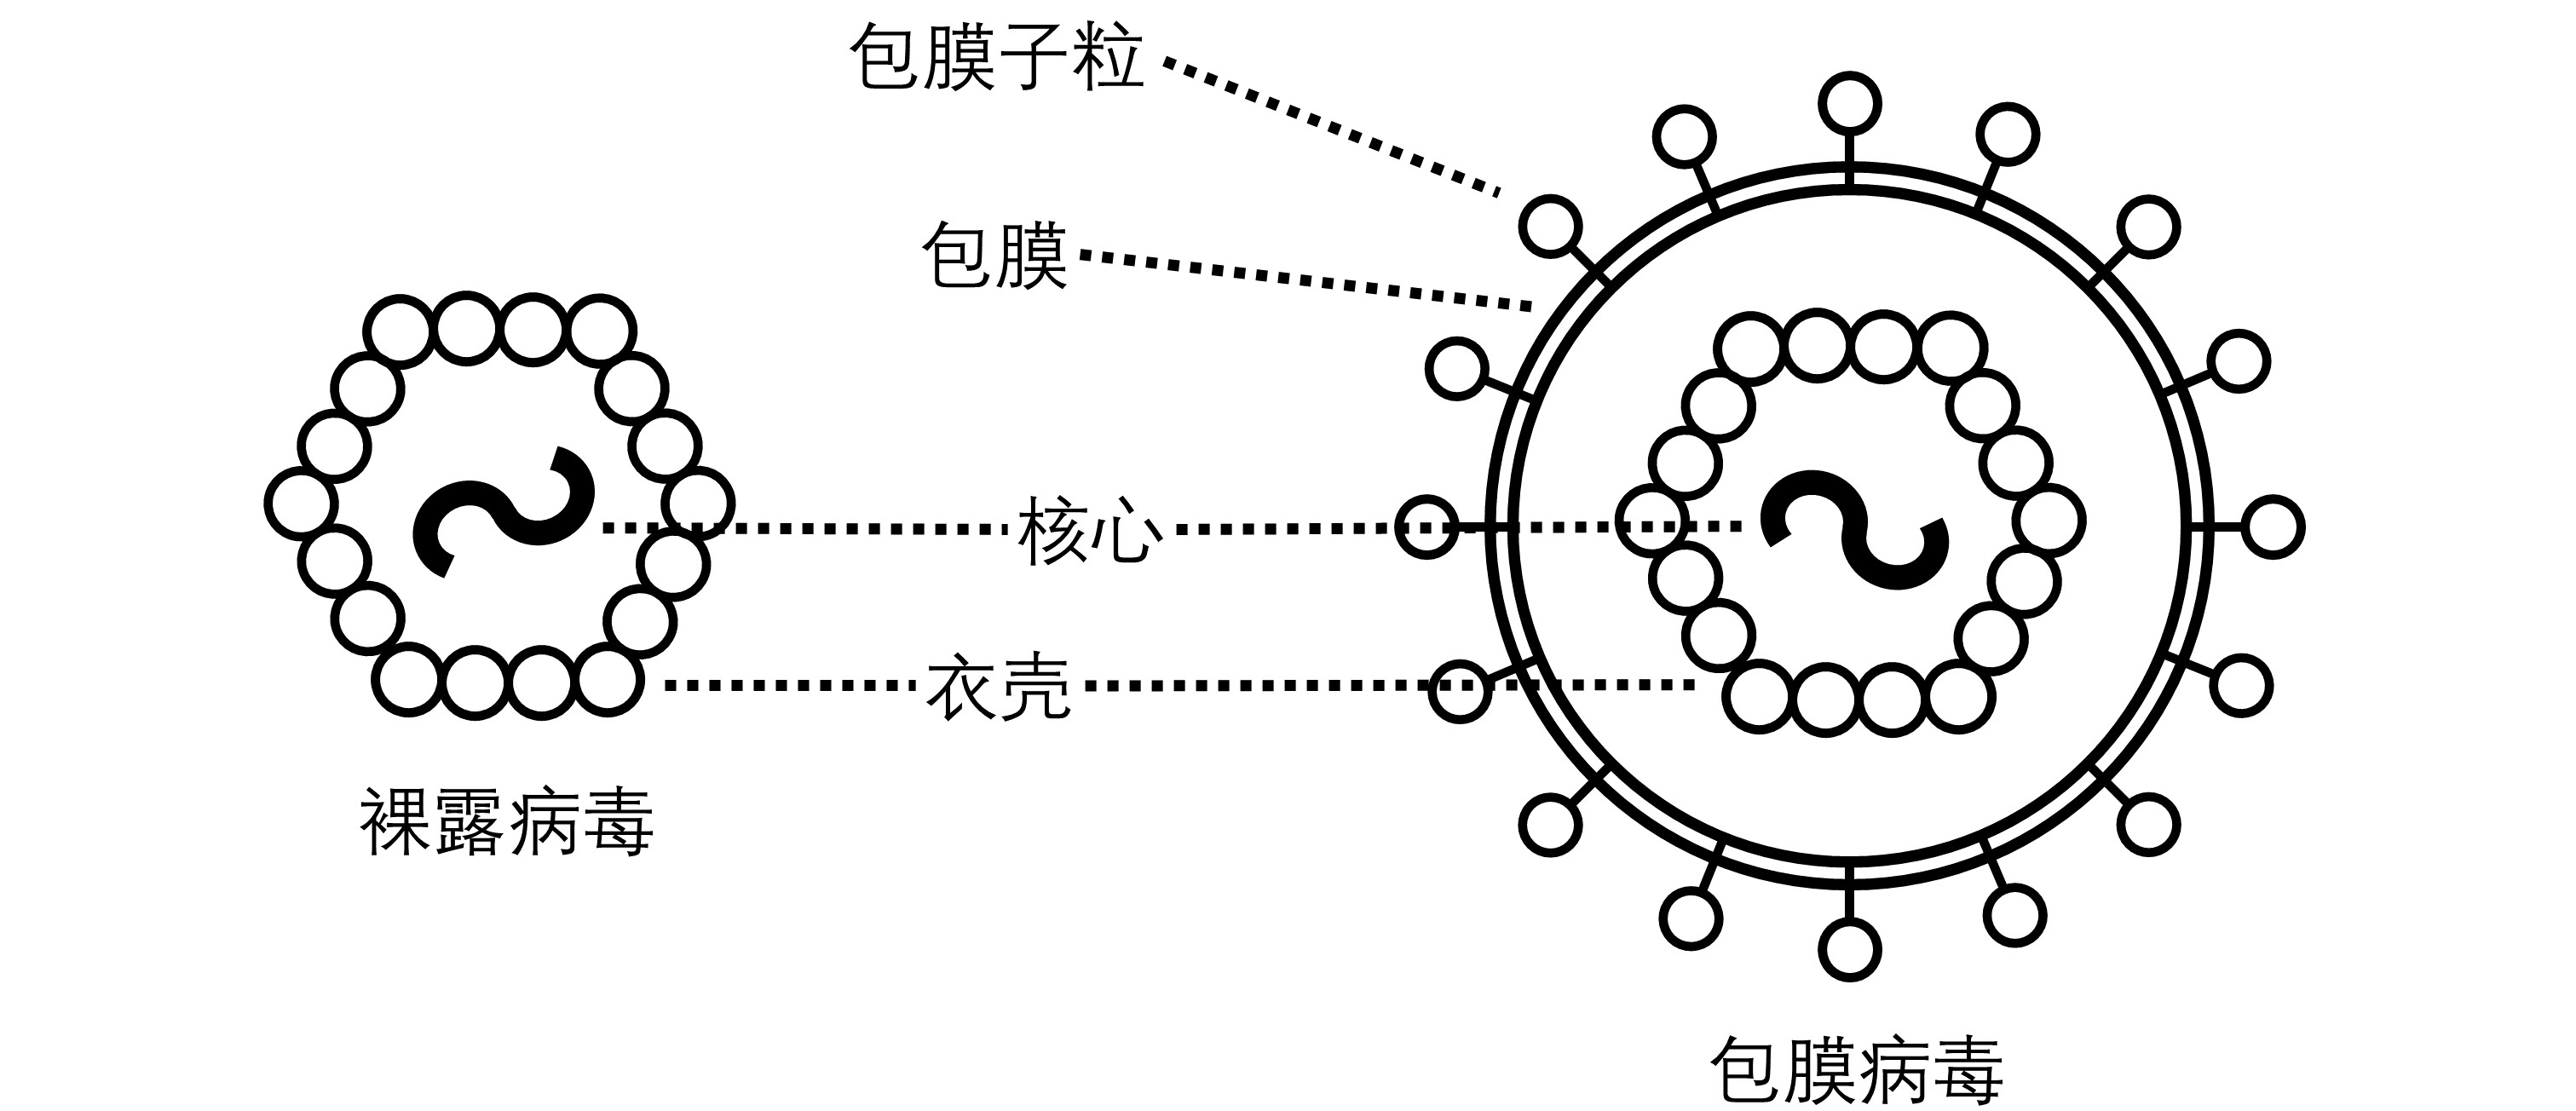
\includegraphics[width=10cm]{BiologyImage/50.jpg}
            \caption{病毒的结构}
        \end{center}
    \end{figure}\\
    病毒入侵宿主细胞的过程分为五步:\\[4mm]
    \textbf{1.吸附:}病毒通过空气或体液等途径进入宿主体内,吸附在宿主的细胞上。\\[4mm]
    \textbf{2.注入:}对于裸露病毒,病毒只会将核酸注入宿主细胞内,蛋白质会留在细胞外。\\[4mm]
    \textbf{2.注入:}对于包膜病毒,包膜会直接于宿主细胞的细胞膜融合,
    核酸和蛋白质会同时进入细胞,在溶酶体的作用下,
    病毒的蛋白质衣壳被水解,从而释放出核酸。\\[4mm]
    \textbf{3.合成:}
    病毒核酸利用细胞内的各类物质,合成自己的核酸和蛋白质。\\[4mm]
    \textbf{4.组装:}
    病毒合成完毕的核酸与蛋白质衣壳结合,组装为新的病毒。\\[4mm]
    \textbf{5.释放:}
    宿主细胞在病毒的作用下发生裂解,内部的大量病毒被释放,继续侵染其他细胞。\\

\subsection{细菌}
    细菌是一类原核生物,无成形的细胞核。\\[6mm]
    细菌有细胞质,细胞膜,细胞壁,但没有细胞核,其细胞质中也只有核糖体一种细胞器。\\[3mm]
    细菌的遗传物质是脱氧核糖核酸,大部分分布在拟核中,少部分分布在质粒中。\\[3mm]
    细菌拟核中的遗传信息主要控制细菌的基本性状。\\[3mm]
    细菌质粒中的遗传信息主要控制细菌的抗药性和物质合成。\\[3mm]
    细菌的质粒是双链环状脱氧核糖核酸分子,质粒不需要整合进入质粒就可以在细菌中直接表达,
    同时细菌可以吞噬环境中散落的质粒,因此细菌非常容易变异。\\[6mm]
    细菌表面生长的较长的毛称为鞭毛,数量较少,可以使细菌具有运动能力。\\[3mm]
    细菌表面生长的较短的毛称为菌毛,数量较多,可以使细菌具有附着于物体表明的能力。\\[6mm]
    下图展示了细菌的结构:
    \begin{figure}[h]
        \begin{center}
            \includegraphics[width=10cm]{BiologyImage/51.jpg}
            \caption{细菌的结构}
        \end{center}
    \end{figure}\\
    当环境不利于细菌生存时,部分细菌可以其外侧形成一层很厚的荚膜,
    同时自身进入休眠状态,变为芽孢,芽孢可以抵抗非常恶劣的环境,
    当环境条件合适时,芽孢会萌发,重新变为细菌。

\newpage

    真细菌指的是通常在常规环境中生存的细菌。\\[3mm]
    古细菌指的是通常在极端环境中生存的细菌。\\[3mm]
    古细菌适应于在极端恶劣的环境中进行生存,例如高温环境,高盐环境,强酸环境,缺氧环境,
    由于这些环境类似于地球形成早期的环境,因此将这一类细菌称为古细菌。\\[3mm]
    以下列出了几种古细菌和其生存环境:
    \begin{table}[h]
        \begin{center}
            \begin{tabular}{l|l}
                \hline
                古细菌类型\qquad\qquad\qquad&生存环境\qquad\qquad\qquad\\ \hline
                嗜热菌&高温环境\\ \hline
                嗜盐菌&高盐环境\\ \hline
                嗜酸菌&强酸环境\\ \hline
                产甲烷细菌&缺氧的粪池\\ \hline
            \end{tabular}
            \caption{古细菌的生存环境}
        \end{center}
    \end{table}\\
    古细菌的抗逆性很强,古细菌的蛋白质和核酸可以耐受高温,古细菌还可以抵抗常规的抗生素。\\[3mm]
    青霉素可以抑制真细菌合成肽聚糖,使其无法形成细胞壁。\\[3mm]
    利福平可以抑制真细菌的核糖体的翻译过程,使其无法合成蛋白质。\\[3mm]
    由于古细菌的细胞壁成分不是肽聚糖,故青霉素对古细菌无效。\\[3mm]
    由于古细菌的翻译过程与真细菌不同,故利福平对古细菌无效。\\[6mm]
    某些细菌可以在极端环境中生存,例如幽门螺旋菌,
    是唯一一种可以在人类胃酸中生存的细菌,
    但实际上幽门螺旋菌是通过不断释放蛋白质来避免菌体受到胃酸腐蚀,
    细胞自身无法承受胃酸,
    若未能在蛋白质释放殆尽前穿过胃黏膜,就会被胃酸杀死。\\[3mm]
    由此可以看出幽门螺旋菌虽然可以勉强在极端环境中生存,
    但并不适合,所以仍然属于真细菌。\\

\subsubsection{细菌在氮循环中的作用}
    细菌在自然界的氮循环中也起到了重要作用:\vspace{5pt}
    \begin{table}[h]
        \begin{center}
            \begin{tabular}{l|l|l|l}
                \hline
                产生\ce{NH4+}\qquad\qquad&固氮菌\qquad\qquad&固氮作用\qquad\qquad&异养好氧\qquad\qquad\\ \hline
                产生\ce{NO2-}\qquad\qquad&亚硝酸细菌\qquad\qquad&硝化作用\qquad\qquad&自养好氧\qquad\qquad\\ \hline
                产生\ce{NO3-}\qquad\qquad&硝酸细菌\qquad\qquad&硝化作用\qquad\qquad&自养好氧\qquad\qquad\\ \hline
                产生\ce{N2}\qquad\qquad&反硝化细菌\qquad\qquad&反硝化作用\qquad\qquad&异养厌氧\qquad\qquad\\ \hline
            \end{tabular}
            \caption{细菌在氮循环中的作用}
        \end{center}
    \end{table}

\newpage

\subsubsection{可以合成人类所需物质的细菌}
    有些细菌可以合成人类所需的物质:\vspace{5pt}
    \begin{table}[h]
        \begin{center}
            \begin{tabular}{l|l|l}
                \hline
                醋酸杆菌\qquad\qquad&合成醋酸\qquad\qquad&异养好氧\qquad\qquad\\ \hline
                乳酸杆菌\qquad\qquad&合成乳酸\qquad\qquad&异养厌氧\qquad\qquad\\ \hline
            \end{tabular}
            \caption{可以合成人类所需物质的细菌}
        \end{center}
    \end{table}\\
    虽然醋酸杆菌和乳酸杆菌的产物均为有机物,
    但是这些有机物并不是通过对无机物的合成产生,
    而是细菌分解了能量价值更高的有机物所得到的产物,
    所以两者的营养方式均为异养。

\subsubsection{可以进行光合作用的细菌}
    有些细菌可以进行原始的光合作用:\vspace{5pt}
    \begin{table}[h]
        \begin{center}
            \begin{tabular}{l|l|l}
                \hline
                蓝细菌\qquad\qquad&光合作用\textbf{产生氧气}\qquad\qquad&自养好氧\qquad\qquad\\ \hline
                光合细菌\qquad\qquad&光合作用\textbf{不产生氧气}\qquad\qquad&自养厌氧\qquad\qquad\\ \hline
            \end{tabular}
            \caption{可以进行光合作用的细菌}
        \end{center}
    \end{table}\\
    虽然这两种细菌均可以进行光合作用,但是细菌并没有除了核糖体外的细胞器,也没有叶绿体,
    它的光合作用是直接通过细菌中的叶绿素进行的,机理也与植物有所不同,较为原始。\\

\subsection{真菌}
    真菌是一类真核生物,有成形的细胞核。

\subsubsection{酵母菌}
    酵母菌属于单细胞真菌,面包和馒头的制作过程,葡萄酒和啤酒的酿造,均需要酵母菌的参与。\\[3mm]
    酵母菌在环境良好时会进行出芽生殖,酵母菌在环境恶劣时会进行孢子生殖。

\subsubsection{霉菌}
    霉菌属于多细胞真菌,腐烂的水果果皮呈现出黑色或绿色实际上就是由于有霉菌的存在所致。\\[3mm]
    霉菌通过孢子繁殖,其孢子可以具体分为无性孢子和有性孢子。

\subsubsection{蕈}
    \ruby{蕈}{x\`un}是一种大型真菌,也就是我们通常意义上的蘑菇。\\[1mm]

\newpage

\subsection{原生生物}
    原生生物指的是真核生物中较为原始的动物或植物。

\subsubsection{植物中的原生生物}
    植物中的原生生物是藻类,与细菌中可以进行光合作用的细菌不同,
    藻类均具有完整的叶绿体,但仍然都是单细胞生物,
    相较于一般意义上的植物还是较为低等。\\[3mm]
    在藻类中,有一部分具备运动能力,例如衣藻,
    另一部分不具备运动能力,例如小球藻。

\subsubsection{动物中的原生生物}
    动物中的原生生物包含草履虫,变形虫等原生动物,
    原生动物大多都是具有一个或多个细胞核,具备运动能力的单细胞生物。
    原生动物是水域中重要的浮游生物,有利于维护生态系统稳定性。

\subsubsection{黏菌}
    黏菌是一种介于原生动物和真菌间的生物,
    没有细胞壁,其营养体具有细胞形态和非细胞形态,
    细胞形态下行为类似于变形虫,非细胞形态下则是一团含有许多细胞核的原生质团。\\[3mm]
    黏菌通过吞噬细菌或有机物颗粒的方式获取能量,黏菌在环境条件较为恶劣时,
    可以长出类似真菌的子实体,并形成孢子,通过孢子进行繁殖。

\subsection{微生物的营养}
    微生物所需的营养可以分为五类:\\[5mm]
    \textbf{水:}
    水是微生物生长代谢不可缺少的物质。\\[6mm]
    \textbf{碳源:}
    碳源是为微生物提供碳元素的物质,
    例如葡萄糖,麦芽糖,纤维素均可以作为碳源。\\[3mm]
    大多数微生物所需的是有机碳源,
    只有部分可以进行光合作用的微生物才能利用无机碳源。\\[3mm]
    一般来说,碳源所需的量相对较多。\\[6mm]
    \textbf{氮源:}
    氮源是为微生物提供氮元素的物质,
    例如氨基酸,嘌呤,嘧啶,铵盐均可以作为氮源。\\[3mm]
    大多数微生物所需的是化合态氮源,
    只有部分可以进行固氮作用的微生物才能利用游离态氮源。\\[3mm]
    一般来说,氮源所需的量相对较少。\\[6mm]
    \textbf{无机盐:}
    无机盐是微生物生长代谢所必须的成分,
    例如磷酸盐,硫酸盐,钠盐,钾盐,钙盐等。\\[6mm]
    \textbf{生长因子:}
    生长因子指的是一类微生物自身无法合成,
    但却是其生长代谢中所必须的微量物质,
    例如某些特定的维生素,某些特定的氨基酸。

\subsection{培养基的配置}
    培养基指的是人工配置的,适合微生物生长繁殖的营养基质。\\[3mm]
    在配置培养基时,会经常的使用两种物质,牛肉膏和蛋白胨,
    这两者均可同时作为碳源和氮源,
    使用这两种物质配置而成的培养基称为“牛肉膏蛋白胨培养基”。\\[6mm]
    培养基按照状态可以分为两类:液体培养基,固体培养基。\\[3mm]
    液体培养基通常用于工业大规模生产。\\[3mm]
    固体培养基通常用于微生物的分离纯化。\\[6mm]
    培养基按照用途可以分为两类:通用培养基,选择培养基。\\[3mm]
    通用培养基指的是可以生长各类微生物的培养基,例如牛肉膏蛋白胨培养基。\\[3mm]
    选择培养基指的是用于选择某种特定微生物的培养基:\\[3mm]
    例如培养基中不加入氮源,
    使得只有能利用空气中\ce{N2},可以进行固氮作用的微生物才能生长。\\[3mm]
    例如培养基中不加入碳源,
    使得只有能利用空气中\ce{CO2},可以进行光合作用的微生物才能生长。\\[3mm]
    例如培养基中加入伊红和美蓝两种染料,
    使得大肠杆菌被染为金属光泽的紫黑色,从而分离。\\[3mm]
    例如培养基中加入青霉素,使得只有具有青霉素抗性基因的微生物生长。\\[6mm]
    微生物的接种有两种方法:平板划线法,平板涂布法。\\[3mm]
    平板划线法使用的工具为接种环,使用前需要灼烧,通常用于单菌落的分离。\\[3mm]
    平板涂布法使用的工具为无菌玻璃刮铲,使用前无需灼烧,通常用于抑菌圈实验。\\

\subsection{传染病的传播}
    传染病的传播分为三个环节:传染源,传播途径,易感人群。
    
\subsubsection{传染源}
    传染源一般是指能将病原体微生物直接传播给宿主的生物。\\[3mm]
    需要指出的是,病原体自身不能称为传染源,病原体感染的生物才能称为传染源。\\[3mm]
    需要注意传染源不分死活,带有鼠疫的田鼠属于传染源,带有鼠疫的田鼠尸体也属于传染源。

\newpage

\subsubsection{传播途径}
    传播途径指的是病原微生物从一个宿主传递到另一个宿主的过程,主要分为四种:\\[6mm]
    \textbf{空气传播:}空气传播指的是病原微生物经病人的咳嗽或喷嚏等途径进入空气,通过飞沫或尘埃,使得病原微生物在空气中进行传播的过程。\\[6mm]
    \textbf{接触传播:}接触传播指的是在接触传染源的过程中受到病原微生物感染的过程。\\[3mm]
    接触传染源的皮肤感染,接触传染源的血液或体液感染,这些均属于接触传播。\\[3mm]
    接触传播并不限于直接接触,在输血过程中若使用受污染的血液受到感染,也属于接触传播。\\[6mm]
    \textbf{病媒传播:}病媒传播指的是通过接触携带病原体微生物的活体而受到感染。\\[3mm]
    例如被带有疟原虫的蚊子叮咬,食用了带有病毒的蝙蝠,属于病媒传播。\\[3mm]
    需要注意携带病原体的活体不应当被感染,仅仅是携带病原体,否则该活体只能算作传染源。\\[6mm]
    \textbf{媒介物传播:}媒介物传播指的是通过接触被传染源污染的无生命物体的过程中受到感染。\\[3mm]
    例如接触了病人使用过的毛巾牙刷,饮用了被污染的水,食用了被污染的食物,属于接触传播。\vspace{3pt}

\subsubsection{易感人群}
    在传染病流行时,有的人会患病,有的人不会患病,我们将容易染病的称为易感人群。\\[1mm]

\subsection{传染病的防治}
    预防传染病,只需要切断由传染源,传播途径,易感人群等环节所构成的传染链:

\subsubsection{控制传染源}
    对于传染源为人类的情况,可以采取隔离和医学观察的方式进行控制。\\[3mm]
    对于传染源为动物的情况,在需要的时候也可以采取大规模扑杀的方式进行控制。

\subsubsection{切断传播途径}
    例如针对通过空气传播的传染病,
    可以采取通风,消毒等方式实现切断传播途径。

\subsubsection{保护易感人群}
    保护易感人群的唯一方式是注射疫苗,
    疫苗可以使接种者获得抗体,
    减少易感人群的数量。

\newpage

\section{人体内环境}

\subsection{体液}
    我们将人体内全部液体总称为体液,
    处于细胞外的称为细胞外液,
    处于细胞内的称为细胞内液,
    其中细胞外液可以分为三类:
    血浆,组织液,淋巴液。\\[6mm]
    血浆存在于血管中,血浆是血细胞生存的环境。\\[3mm]
    血浆中含量最多的物质是血浆蛋白,血浆中同时还包含一些有机物以及无机离子。\\[3mm]
    需要指出的是,血浆蛋白存在于血浆中,血红蛋白存在于血细胞中,两者是完全不同的。\\[6mm]
    组织液存在于组织细胞间,组织液是组织细胞生存的环境。\\[3mm]
    组织液会从细胞中吸取代谢废物,细胞会从组织液中吸取营养物质。\\[3mm]
    组织液会从血浆中吸取营养物质,血浆会从组织液中吸取代谢废物。\\[3mm]
    组织液和血浆间可以进行物质交换,除了大分子蛋白无法通过血管壁外,其他物质均可以通过。\\[6mm]
    淋巴液存在于淋巴管中,淋巴液是淋巴细胞生存的环境。\\[3mm]
    组织液可以通过毛细淋巴管的盲端加入淋巴液,
    盲端管壁的细胞间隙很大,所有物质均可通过,
    但只允许物质从组织液进入淋巴液,
    而不允许物质从淋巴液返回组织液。\\[3mm]
    淋巴液会顺着淋巴管流动,最终回流至血管。\\
    \begin{figure}[h]
        \begin{center}
            \includegraphics[width=10cm]{BiologyImage/52.jpg}
        \end{center}
        \caption{血浆~~组织液~~淋巴液}
    \end{figure}\\
    血浆,组织液,淋巴液,三者通过动态的有机联系,
    共同构成了人体大多数细的生存环境。\\[3mm]
    我们将由细胞外液构成的液体环境称为内环境。

\newpage

\subsection{渗透压}
    溶液的渗透压与溶质微粒的多少有关,在水的量一定时:\\[3mm]
    溶质微粒越多,浓度越高,渗透压越高。\\[3mm]
    溶质微粒越少,浓度越低,渗透压越低。\\[3mm]
    水分倾向于从渗透压低处向渗透压高处流动。\\[3mm]
    如果静脉注射了浓度偏低,也就是渗透压较低的水溶液,
    由于红细胞内部的渗透压高于外部,
    水由渗透压低的外部向渗透压高的内部流动,
    导致红细胞大量吸水破裂。\\[3mm]
    如果静脉注射了浓度偏低,也就是渗透压较低的水溶液,
    由于红细胞内部的渗透压高于外部,
    水由渗透压低的内部向渗透压高的外部流动,
    导致红细胞大量失水萎缩。\\[3mm]
    人体中的渗透压主要由以下离子维持:\vspace{5pt}
    \begin{table}[h]
        \begin{center}
            \begin{tabular}{l|l|l}
                \hline
                体液\qquad\qquad&阳离子\qquad\qquad\qquad&阴离子\qquad\qquad\qquad\qquad\qquad\\ \hline
                细胞内液&\ce{K+}&\ce{HPO4^{2-}}~~~~\ce{H2PO4-}\\ \hline
                细胞外液&\ce{Na+}&\ce{Cl-}\\ \hline            
            \end{tabular}
            \caption{维持人体渗透压的粒子}
        \end{center}
    \end{table}\\
    除此之外,蛋白质在细胞内液中也可以作为阴离子起到维持渗透压的作用。\\

\subsection{酸碱度}
    人体内环境的ph值通常在$7.4$左右,
    如果酸碱度低于$7.0$或高于$7.8$,人会在几分钟内死亡。\\[3mm]
    细胞外液的酸碱度主要由呈弱酸性的碳酸(\ce{H2CO3})和呈弱碱性的碳酸氢钠(\ce{NaHCO3})维持。\\[6mm]
    当遇到酸性较强的物质时,
    细胞外液中的\ce{NaHCO3}会与其反应,
    生成酸性较弱的\ce{H2CO3}:
    \begin{center}
        \ce{NaHCO3 + HL -> NaL + H2CO3}
    \end{center}
    \vspace{5pt}
    当遇到碱性较强的物质时,
    细胞外液中的\ce{H2CO3}会与其反应,
    生成碱性较弱的\ce{NaHCO3}:
    \begin{center}
        \ce{H2CO3 + Na2CO3 -> 2NaHCO3}
    \end{center}
    \vspace{8pt}
    对于多余的碳酸(\ce{H2CO3})和碳酸氢钠(\ce{NaHCO3}):\\[3mm]
    当碳酸过多时,肾脏会选择更多的回收碳酸氢钠,同时更多的滤出碳酸。\\[3mm]
    当碳酸氢钠过多时,肾脏会选择更多的回收碳酸,同时更多的滤出碳酸氢钠。\\[3mm]
    另外有一部分碳酸也会分解为水和二氧化碳,二氧化碳会随着呼吸排出体外。

\newpage

\subsection{产热和散热}
    人体的体温通常恒定在37$^{\circ}$C左右,
    体温过高或过低会影响酶活性,
    从而影响新陈代谢的进行,
    最终导致器官的功能紊乱,严重时还会危及生命。\\[3mm]
    人体体温的维持主要依靠产热和散热,通常情况下,
    产热量和散热量是相等的。
    
\subsubsection{产热}
    人在运动时,产热量主要来自骨骼肌的活动。\\[3mm]
    人在安静时,产热量则主要来自内脏,其中肝脏的产热量尤其高。\\[3mm]
    运动时的产热量是安静时的的$10$-$15$倍。

\subsubsection{散热}
    人的散热主要是依靠皮肤完成,皮肤的散热有四种方式:传导,对流,辐射,蒸发。\\[6mm]
    \textbf{传导散热:}
    传导散热指的是通过热传导的方式放出热量。\\[3mm]
    例如使用冰袋为高烧病人降温。\\[6mm]
    \textbf{对流散热:}
    对流散热指的是通过热对流的方式放出热量。\\[3mm]
    例如在夏天使用电风扇就是通过气体对流从而带走了人体产生的热量。\\[6mm]
    \textbf{辐射散热:}
    对流散热指的是通过热辐射的方式放出热量。\\[3mm]
    例如在夏天通过伸展四肢睡觉以促进辐射散热,
    例如在冬天通过蜷缩身体睡觉以减少辐射散热。\\[6mm]
    \textbf{蒸发散热:}
    蒸发散热指的是通过水的蒸发带走热量。\\[3mm]
    蒸发散热是唯一一种能在外界温度高于体温时可以工作的散热方式。\\[4mm]

\newpage
    
\subsection{渗透压的调节}
    人体的渗透压由下丘脑渗透压中枢调节。\\[3mm]
    当人体内血浆含水量偏高时,会导致血浆渗透压偏低,
    下丘脑从而会减少抗利尿激素的分泌量,
    抗利尿激素的减少会导致肾脏对水的重吸收作用减弱,
    使排尿量增加,排出水分。\\[3mm]
    当人体内血浆含水量偏高时,会导致血浆渗透压偏高,
    下丘脑从而会增加抗利尿激素的分泌量,
    抗利尿激素的增加会导致肾脏对水的重吸收作用增强,
    使排尿量减少,保留水分。\\[3mm]
    同时下丘脑渴觉中枢兴奋,饮水量增加,补充水分。
    \begin{figure}[h]
        \begin{center}
            \includegraphics[width=14cm]{BiologyImage/53.jpg}
        \end{center}
        \caption{渗透压的调节}
    \end{figure}

\newpage

\subsection{体温的调节}
    人体的体温由下丘脑体温调节中枢控制。\\[3mm]
    下丘脑体温调节中枢可以通过四种方式调节散热量:\\[3mm]
    皮肤血管的收缩与舒张,汗腺分泌的增强与减弱,立毛肌的收缩,骨骼肌的战栗。\\[3mm]
    下丘脑体温调节中枢可以通过两种方式调节产热量:\\[3mm]
    肾上腺分泌的肾上腺素的多少,甲状腺分泌的甲状腺素的多少。\vspace{10pt}
    \begin{figure}[h]
        \begin{center}
            \includegraphics[width=14cm]{BiologyImage/54.jpg}
        \end{center}
        \caption{体温的调节}
    \end{figure}

\newpage

\subsection{血糖的调节}
    人体的血糖调节由下丘脑糖中枢控制。\\[3mm]
    当人体血糖浓度偏高时,会导致胰岛B细胞分泌的胰岛素增加,促使血糖浓度下降。\\[3mm]
    当人体血糖浓度偏低时,会导致胰岛A细胞分泌的胰高血糖素素增加,促使血糖浓度升高。\\[3mm]
    同时下丘脑糖中枢通过神经调节使肾上腺素分泌增加,促使血糖浓度升高。\\[3mm]
    此外下丘脑糖中枢通过体液调节使肾上腺皮质激素分泌增加,促使血糖浓度升高。\\[3mm]
    需要指出的是,肾上腺皮质激素只能促进非糖物质转化为糖,无法促进肝糖原的分解。\\[3mm]
    胰岛A细胞和胰岛B细胞既可以直接感受血糖的变化,也可以受下丘脑糖中枢的神经调控。\\[3mm]
    在血糖浓度过低(低于$3.33$~mmol/L~)的紧急情况下,
    下丘脑糖中枢兴奋,直接通过神经调节,
    刺激肝细胞分解肝糖原,从而快速提高血糖。\vspace{15pt}
    \begin{figure}[h]
        \begin{center}
            \includegraphics[width=14cm]{BiologyImage/55.jpg}
        \end{center}
        \caption{血糖的调节}
    \end{figure}

\newpage

\subsection{血脂的代谢}
    血液中的脂质称为血脂,由于脂质不溶于水,所以血脂均是以脂蛋白的形式存在于血液中。\\[3mm]
    脂蛋白由蛋白质分子,磷脂分子,胆固醇分子,甘油三酯分子组成。\\[3mm]
    脂蛋白中的磷脂以磷脂单分子层的形式存在,亲水端对外接触血液,疏水端对内接触甘油三酯。\\[3mm]
    血脂可以具体分为四类:\vspace{5pt}
    \begin{table}[h]
        \begin{center}
            \begin{tabular}{l|l|l}
                \hline
                名称\qquad\qquad\qquad&简写\qquad\qquad\qquad&主要携带物质\qquad\qquad\qquad\\ \hline
                乳糜颗粒&CM&甘油三酯\\ \hline
                极低密度脂蛋白&VLDL&甘油三酯\\ \hline
                低密度脂蛋白&LDL&胆固醇\\ \hline
                高密度脂蛋白&HDL&胆固醇\\ \hline
            \end{tabular}
        \end{center}
        \caption{血脂的分类}
    \end{table}\\
    四者按前后顺序,密度逐渐变大,体积逐渐减小。\\[3mm]
    甘油三酯以CM的形式由小肠进入血管,以VLDL的形式由肝脏进入血管。\\[3mm]
    甘油三酯主要储存在脂肪细胞,只有极少部分储存在肝脏细胞。\\[3mm]
    胆固醇以LDL的形式运入组织细胞,以HDL的形式运出组织细胞。\\[3mm]
    胆固醇大部分由肝脏合成,少部分从食物中获取,在肝脏中HDL将被加工为胆汁酸排出体外。\vspace{5pt}
    \begin{figure}[h]
        \begin{center}
            \includegraphics[width=14cm]{BiologyImage/56.jpg}
        \end{center}
        \caption{血脂的代谢}
    \end{figure}

\newpage

\subsection{血压的调节}
    心血管系统是一个封闭的管道系统,在血管种有足够的血液充盈,这是形成血压的一个前提。\\[3mm]
    心脏在血液循环系统种起到了泵的作用,心室肌收缩将血液从左心室射入主动脉,
    血液对主动脉壁产生了侧压,这就是动脉血压,一般意义上的血压指的均是动脉血压。\\[3mm]
    心室收缩中期时,主动脉上的血压最高,此时的动脉血压称为收缩压。\\[3mm]
    心室舒张末期时,主动脉上的血压最低,此时的动脉血压称为舒张压。\\[3mm]
    收缩压和舒张压之间的差值称为脉压。\\[6mm]
    动脉血压的形成主要是源于两个因素,心室射血和外周阻力:\\[3mm]
    如果心脏收缩时向动脉射入更多血液,心排血量增大,动脉血压升高。\\[3mm]
    如果血管半径减小或血液粘滞度增高,外周阻力增大,动脉血压升高。\\[6mm]
    人体的血压中枢受位于脑干的心血管中枢调控。\\[3mm]
    血压较高时,降压反射强,冲动传递至心血管中枢,导致副交感神经兴奋。\\[3mm]
    此时通过神经调节,心率减慢,心排血量减少,血管平滑肌舒张,外周阻力减少,血压下降。\\[3mm]
    血压较低时,降压反射弱,冲动传递至心血管中枢,导致交感神经兴奋。\\[3mm]
    此时通过神经调节,心率加快,心排血量增加,血管平滑肌收缩,外周阻力增加,血压升高。\\[6mm]
    主动脉的管壁具有显著的弹性:\\[3mm]
    心脏收缩时,主动脉扩张,缓冲心脏射血的压力,使收缩压不至于过高,\\[3mm]
    心脏舒张时,主动脉回缩,继续推动血液的前进,使舒张压不至于过低。

\newpage

\subsection{糖尿病}
    糖尿病指的是由于胰岛素异常而导致血糖浓度偏高的一种疾病,
    当血糖浓度超过$9$~mmol/L时,葡萄糖将会从尿液中排出,形成尿糖,所以这种病被称为糖尿病。\\[6mm]
    糖尿病按照其发病原因可以分为两类:\\[3mm]
    1型糖尿病:胰岛素分泌绝对不足,
    发病与遗传因素和病毒感染有关,
    这些因素导致胰岛受损,使得胰岛B细胞数量减少,从而导致胰岛素分泌量不足。\\[2mm]
    1型糖尿病占糖尿病患者的10\%,多发病与青少年。\\[2mm]
    1型糖尿病需要通过注射胰岛素治疗。\\[4mm]
    2型糖尿病:胰岛素分泌相对不足,
    发病与过度肥胖,高血压,高血脂,不良的生活习惯有关,
    通常存在胰岛素抵抗,例如胰岛素受体无法与胰岛素结合,
    使胰岛素无法发挥作用。\\[2mm]
    2型糖尿病占糖尿病患者的90\%,多发病与中老年。\\[2mm]
    2型糖尿病需要通过服用降糖药治疗,同时需要控制饮食,增加运动。\\[6mm]
    糖尿病会导致一系列急性和慢性的并发症:
    脑中风,心脏病,肾脏病,失明,下肢坏疽。\\[3mm]
    糖尿病患者会出现“三多一少”症状:排尿量增多,饮水量增多,摄食量增多,体重减轻。\\[3mm]
    由于血浆中葡萄糖浓度很高,使得经过滤过作用产生的原尿葡萄糖浓度仍然很高,
    导致葡萄糖的重吸收作用受阻,进一步影响了水的重吸收,从而导致排尿量增多。\\[3mm]
    由于机体排尿量增多,血浆的含水量下降,血浆的渗透压上升,导致渴觉中枢兴奋,
    产生渴觉,从而促进机体大量饮水,导致饮水量增多。\\[3mm]
    由于葡萄糖大量的通过尿液排出,
    机体对血糖的利用非常少,导致摄食中枢兴奋,产生饥饿感,
    于是大量摄入食物,从而导致摄食量增多。\\[3mm]
    由于葡萄糖无法被机体所利用,导致脂肪无法堆积,
    同时还迫使机体不断分解脂肪和肌肉组织,
    以维持生命活动所需的能量,从而导致体重减轻。

\newpage
    
\subsection{高血脂}
    高血脂指的是由于血脂来源增加或去路减少,
    导致血脂浓度过高的一种疾病。\\[6mm]
    高血脂可以具体分为三类:\\[3mm]
    \textbf{单纯性高甘油三酯血症:}
    主要与运输甘油三酯的乳糜颗粒和极低密度脂蛋白异常有关。\\[2mm]
    乳糜颗粒合成增加导致血脂来源增加,极低密度脂蛋白合成增加导致血脂来源增加。\\[3mm]
    \textbf{单纯性高胆固醇血症:}
    主要与运输胆固醇的低密度脂蛋白和高密度脂蛋白异常有关。\\[2mm]
    低密度脂蛋白合成增加导致血脂来源增加,高密度脂蛋白合成减少导致血脂去路减少。\\[3mm]
    \textbf{两者兼有的血脂代谢紊乱性疾病:}同时存在甘油三酯和胆固醇的异常。\\[6mm]
    高血脂的病因较复杂,有先天因素导致的,
    例如家族性高胆固醇血症或家族性高甘油三酯血症,有后天因素导致的,
    例如高糖高脂饮食,长期吸烟,大量饮酒,运动量少。\\[3mm]
    高血脂直接导致动脉粥样硬化,其中,
    甘油三脂会沉积在血管壁上,
    胆固醇会沉积在血管壁内,
    两者均会导致血管壁狭窄,血流减慢,
    造成机体各种组织器官供血不足。\\[3mm]
    如果心脏供血不足,会导致心肌梗死,
    如果大脑供血不足,会导致脑梗死。\\

\subsection{高血压}
    高血压指的是在未服用药物的情况下,
    收缩压大于等于$140$~mmHg或舒张压大于等于$90$~mmHg。\\[3mm]
    高盐饮食是导致高血压的主要因素,
    摄入的无机盐使血浆渗透压升高,
    肾小管重吸收作用加强,
    血容量增多,血液对血管壁侧压增强,
    从而导致高血压。\\[3mm]
    高脂饮食是导致高血压的次要因素,
    摄入的甘油三酯和胆固醇堆积在血管壁中,
    血管半径减小,
    外周阻力增大,
    从而导致高血压。\\[3mm]
    遗传因素也能导致高血压。

\newpage

\section{遗传与变异}

\subsection{基因}
    基因是携带遗传信息,并具有遗传效应的脱氧核糖核酸片段。\\[3mm]
    基因的本质是脱氧核苷酸序列,每个脱氧核糖核酸分子中都包含众多基因。\\[3mm]
    基因的脱氧核苷酸序列决定了基因所携带的遗传信息。\\[3mm]
    基因可以通过转录翻译的过程,控制蛋白质的合成,从而控制生物体的性状。\\[3mm]
    我们将位于一对同源染色体同一位置上的一对基因称为等位基因。\\

\subsection{基因分离定律}
    \textbf{基因分离定律:}在减数第一次分裂中,成对的同源染色体分离,成对的等位基因随之分离。\\[3mm]
    下图表现了基因分离定律的过程:
    \begin{figure}[h]
        \begin{center}
            \includegraphics[width=14cm]{BiologyImage/57.jpg}
        \end{center}
        \caption{基因分离定律}
    \end{figure}\\[1mm]
    需要指出的是,基因分离定律是关于一对等位基因的遗传定律。

\newpage

\subsection{基因自由组合定律}
    \textbf{基因自由组合定律:}减数第一次分裂中,不同染色体上的非等位基因之间表现为自由组合。\\[3mm]
    下图表现了基因自由组合定律的过程:\vspace{10pt}
    \begin{figure}[h]
        \begin{center}
            \includegraphics[width=14cm]{BiologyImage/58.jpg}
        \end{center}
        \caption{基因自由组合定律}
    \end{figure}\\[1mm]
    需要指出的是,基因自由组合定律是关于多对等位基因的遗传定律。\\[3mm]
    需要说明的是,基因自由组合定律中的多对等位基因,应当处于不同的染色体上。

\newpage

\subsection{基因连锁交换定律}
    \textbf{基因连锁交换定律:}在减数第一次分裂中,同一染色体上的非等位基因之间表现为连锁,同时,
    在联会过程中,同源染色体上的染色单体之间可能会发生染色体片段的交换。\\[3mm]
    下图表现了基因连锁交换定律的过程:\vspace{10pt}
    \begin{figure}[h]
        \begin{center}
            \includegraphics[width=14cm]{BiologyImage/59.jpg}
        \end{center}
        \caption{基因连锁交换定律}
    \end{figure}\\[1mm]
    需要指出的是,基因连锁交换定律是关于多对等位基因的遗传定律。\\[3mm]
    需要说明的是,基因连锁交换定律中的多对等位基因,应当处于相同的染色体上。

\newpage

\subsubsection{连锁基因的交换情况}
    染色体片端的交换分为三种情况:\\[3mm]
    第一种情况:两个基因都未交换,这种情况属于不发生交换。\\[3mm]
    第二种情况:两个基因中,一个被交换,一个未交换,这种情况属于发生交换。\\[3mm]
    第三种情况:两个基因都被交换,这种情况属于不发生交换。\\[3mm]
    对于第三种情况,虽然两个基因都被交换,但是对配子的比例没有影响,因此归为不发生交换。\\[6mm]
    下图表现了连锁基因的交换:\vspace{5pt}
    \begin{figure}[h]
        \begin{center}
            \includegraphics[width=10cm]{BiologyImage/60.jpg}
        \end{center}
        \caption{连锁基因的交换}
    \end{figure}\\
    从图中我们可以看出:\\[3mm]
    两个连锁基因相距越近,交换概率越小。\\[3mm]
    两个连锁基因相距越远,交换概率越大。

\newpage

\subsubsection{连锁基因的交换值}
    我们可以通过两个角度来衡量交换的概率大小:\\[3mm]
    1.联会时同源染色体的染色单体发生交换的概率,用$\alpha$表示。\\[3mm]
    2.减数分裂产生的配子基因型不同于亲本的比例,用$\beta$表示。\\[6mm]
    两者之间存在一个重要关系:
    \begin{large}
        \begin{equation*}
            \alpha=2\cdot\beta
        \end{equation*}
    \end{large}\\
    我们将配子中基因型与亲本基因型相同的,称为亲本型。\\[3mm]
    我们将配子中基因型与亲本基因型不同的,称为重组型。\\[3mm]
    我们将$\beta$称为连锁基因的交换值。\\[8mm]
    考虑以下两种极端情况:\vspace{5pt}
    \begin{table}[h]
        \begin{center}
            \begin{tabular}{l|l|l|l|l|l}
                \hline
                $\alpha$的取值\qquad\qquad&$\beta$的取值\qquad\qquad&亲本型1\qquad&亲本型2\qquad&重组型1\qquad&重组型2\qquad\\ \hline
                $\,0\%$&$0\%$&$50\%$&$50\%$&$0\%$&$0\%$\\ \hline
                $100\%$&$50\%$&$25\%$&$25\%$&$25\%$&$25\%$\\ \hline
            \end{tabular}
            \caption{两种极端情况的比例}
        \end{center}
    \end{table}\\
    由此可见,交换值$\beta$的取值范围为$0\%-50\%$。\\[3mm]
    我们将交换值满足$\beta=0$的称为基因完全连锁。\\[3mm]
    我们将交换值满足$\beta\neq 0$的称为基因不完全连锁。\\[3mm]
    大部分生物都是不完全连锁,少部分生物是完全连锁,例如雄果蝇和雌家蚕。

\newpage

\subsection{基因和性状的关系}
    我们将控制显性性状的基因称为显性基因,通常用大写英文字母表示,例如\texttt{A}。\\[3mm]
    我们将控制隐性性状的基因称为隐性基因,通常用小写英文字母表示,例如\texttt{a}。\\[3mm]
    等位基因表现形式通常有两种,既可以是显性基因,也可以是隐性基因。

\subsubsection{完全显性}
    在完全显性中,显性基因对隐性基因较为强势,同时存在两者时表现为显性性状。\\[3mm]
    下表展示了完全显性的特点:
    \begin{table}[h]
        \begin{center}
            \begin{tabular}{l|l}
                \hline
                基因型\qquad\qquad\qquad&表现型\qquad\qquad\qquad\\ \hline
                \texttt{AA}&紫花\\ \hline
                \texttt{Aa}&紫花\\ \hline
                \texttt{aa}&白花\\ \hline
            \end{tabular}
            \caption{完全显性(豌豆花色)}
        \end{center}
    \end{table}\vspace{-20pt}

\subsubsection{不完全显性}
    在不完全显性中,显性基因对隐性基因较为弱势,同时存在两者时表现为中间性状。\\[3mm]
    下表展示了不完全显性的特点:
    \begin{table}[h]
        \begin{center}
            \begin{tabular}{l|l}
                \hline
                基因型\qquad\qquad\qquad&表现型\qquad\qquad\qquad\\ \hline
                \texttt{AA}&红花\qquad\\ \hline
                \texttt{Aa}&粉花\qquad\\ \hline
                \texttt{aa}&白花\qquad\\ \hline
            \end{tabular}
            \caption{不完全显性(金鱼草花色)}
        \end{center}
    \end{table}\vspace{-20pt}

\subsubsection{镶嵌显性}
    在镶嵌显性中,显性基因和隐性基因控制的是两个部分,互不遮盖。\\[3mm]
    下表展示了镶嵌显示的特点:
    \begin{table}[h]
        \begin{center}
            \begin{tabular}{l|l}
                \hline
                基因型\qquad\qquad\qquad&表现型\qquad\qquad\qquad\\ \hline
                \texttt{AA}&前端有黑色~~后端无黑色\\ \hline
                \texttt{Aa}&前端有黑色~~后端有黑色\\ \hline
                \texttt{aa}&前端无黑色~~后端有黑色\\ \hline
            \end{tabular}
            \caption{镶嵌显性(异色瓢虫色斑)}
        \end{center}
    \end{table}

\newpage

\subsubsection{复等位基因}
    复等位基因指的是等位基因的表现形式超过两种,即不局限于显性基因和隐性基因。\\[3mm]
    复等位基因是由基因突变造成的,各个基因间的关系较为复杂,由具体情况决定。\\[3mm]
    下表展示了复等位基因的特点:
    \begin{table}[h]
        \begin{center}
            \begin{tabular}{l|l}
                \hline
                基因型\qquad\qquad\qquad&表现型\qquad\qquad\qquad\\ \hline
                \texttt{I$^{\texttt{A}}$I$^{\texttt{B}}$}&AB型血\\ \hline
                \texttt{I$^{\texttt{A}}$I$^{\texttt{A}}$}&A型血\\ \hline
                \texttt{I$^{\texttt{B}}$I$^{\texttt{B}}$}&B型血\\ \hline
                \texttt{I$^{\texttt{A}}$i}&A型血\\ \hline
                \texttt{I$^{\texttt{B}}$i}&B型血\\ \hline
                \texttt{ii}&O型血\\ \hline
            \end{tabular}
            \caption{复等位基因(人类血型)}
        \end{center}
    \end{table}\\
    在人类血型的例子中:\\[3mm]
    基因I$^{\texttt{A}}$对基因i表现为显性。\\[3mm]
    基因I$^{\texttt{B}}$对基因i表现为显性。\\[3mm]
    基因I$^{\texttt{A}}$和基因I$^{\texttt{B}}$间表现为平等。\\[6mm]
    人类血型和凝集原和凝集素有关,凝集原存在于红细胞表面,凝集素存在于血清中。\\[3mm]
    人类血型保证了对应的凝集原和凝集素不会同时存在,但若进行错误输血,则会导致两者相遇,
    造成凝集反应的发生,严重时可导致输血者死亡,因此为保证安全输血应遵循同型输血的原则。\\[3mm]
    下表列出各个血型所具有的凝集原和凝集素:\vspace{3pt}
    \begin{table}[h]
        \begin{center}
            \begin{tabular}{l|l|l}
                \hline
                血型\qquad\qquad&凝集原\qquad\qquad\qquad\qquad&凝集素\qquad\qquad\qquad\qquad\\ \hline
                AB型血&凝集原A~~~~凝集原B\qquad\qquad&无\\ \hline
                A型血&凝集原A&凝集素抗B\\ \hline
                B型血&凝集原B&凝集素抗A\\ \hline
                O型血&无&凝集素抗A~~~~凝集素抗B\qquad\qquad\\ \hline
            \end{tabular}
            \caption{人类血型对应的凝集原与凝集素}
        \end{center}
    \end{table}\vspace{-20pt}

\subsubsection{多基因遗传}
    多基因遗传指的是等位基因的数量不止一对,即多对等位基因控制同一性状。\\[3mm]
    多基因遗传中每一对等位基因的作用都较小,因此可以产生连续变化,也容易受到环境影响。

\newpage

\subsection{伴性遗传}
    性别是由性染色体决定的,通常的性别决定类型有XY型和ZW型:\\[3mm]
    XY型性别决定:雄性为XY,雌性为XX,雄性的精子对子代性别起决定作用。\\[3mm]
    ZW型性别决定:雄性为ZZ,雌性为ZW,雌性的卵子对子代性别起决定作用。\\[3mm]
    包括人在内的绝大多数生物均是XY型性别决定,只有鸟类和爬行类是ZW型性别决定。\\[3mm]
    需要特别说明的是,果蝇属于XY性别决定,家蚕属于ZW性别决定。\\[9mm]
    性染色体上除了有决定性别的基因外,还有一些其他基因。\\[3mm]
    显然这一部分基因在遗传上必然和性别有关,所以将其称为伴性遗传。\\[6mm]
    伴性遗传可以细分为三类:\\[4mm]
    \textbf{伴X染色体隐性遗传(X连锁隐形遗传)}:基因位于X染色体上,且为隐性,
    如果某女性表现出伴X隐性性状,意味着其基因型为$\text{X}^{\text{b}}\text{X}^{\text{b}}$,
    其父亲和儿子的基因型为$\text{X}^{\text{b}}\text{Y}$。\\[2mm]
    所以如果女性表现出伴X染色体隐性性状,其父亲和儿子也必然会表现出该性状。\\[6mm]
    \textbf{伴X染色体显性遗传(X连锁显形遗传)}:基因位于X染色体上,且为显性,
    如果某男性表现出伴X显性性状,意味着其基因型为$\text{X}^{\text{B}}\text{Y}$,
    其母亲和女儿基因型为$\text{X}^{\text{B}}\text{X}^{\text{b}}$或$\text{X}^{\text{B}}\text{X}^{\text{B}}$。\\[2mm]
    所以如果男性表现出伴X染色体显性性状,其母亲和女儿也必然会表现出该性状。\\[6mm]
    \textbf{伴Y染色体遗传(Y连锁遗传)}:基因位于Y染色体上,而只有男性才具有Y染色体。\\[2mm]
    所以伴Y染色体遗传的性状只可能出现于男性。

\newpage

\subsubsection{无籽西瓜的培育}
    下图展示了无籽西瓜的培育过程:\vspace{5pt}
    \begin{figure}[h]
        \begin{center}
            \includegraphics[width=12cm]{BiologyImage/61.jpg}
        \end{center}
        \caption{无籽西瓜的培育}
    \end{figure}\\

\subsubsection{无籽番茄的培育}
    下图展示了无籽番茄的培育过程:\vspace{5pt}
    \begin{figure}[h]
        \begin{center}
            \includegraphics[width=12cm]{BiologyImage/62.jpg}
        \end{center}
        \caption{无籽番茄的培育}
    \end{figure}\\

\newpage

\subsection{基因重组}
    \textbf{基因重组}:在有性生殖的过程中,
    控制不同性状的基因重新组合,使得后代出现新的基因型。\\[3mm]
    基因重组可以发生于基因自由组合定律,由于在减数分离中,非同源染色体间表现为自由组合,
    因此可能会出现新的基因型,所以基因自由组合定律中可能会发生基因重组。\\[3mm]
    基因重组可以发生于基因连锁交换定律,由于在联会过程中,同源染色体间会交换染色体片段,
    因此可能会出现新的基因型,所以基因连锁交换定律中可能会发生基因重组。\\[3mm]

\subsection{基因突变}
    \textbf{基因突变:}在DNA复制过程中,
    碱基对发生替换,缺失,增加而使碱基序列发生改变。\\[3mm]
    基因突变具有稀有性:
    基因突变对单个细胞是稀有的。\\[2mm]
    基因突变具有普遍性:
    基因突变对生物体是普遍的。\\[2mm]
    基因突变具有随机性:基因A有可能突变为基因$\text{a}_\text{1}$,基因$\text{a}_\text{2}$,基因$\text{a}_\text{3}$。\\[2mm]
    基因突变具有可逆性:基因A有可能突变为基因a\,\,\,,基因a也有可能突变为基因A。\\

\subsection{染色体畸变}
    染色体畸变分为染色体结构变异和染色体数目变异。\\[6mm]
    染色体结构变异分为四类:\\[3mm]
    缺失:染色体中某一片段缺少。\\[3mm]
    重复:染色体中某一片段重复。\\[3mm]
    倒位:染色体中某一片段颠倒。\\[3mm]
    易位:染色体移接了一段非同源染色体的片段。\\[6mm]
    染色体数目变异分为两类:\\[3mm]
    染色体非整倍化变异:单个染色体的数目发生变异,这一类变异通常是有害的。\\[3mm]
    染色体整倍化变异:所有染色体的数目发生变异,即体细胞中含有多个染色体组,称为多倍体。\\[3mm]
    多倍体这在植物中非常常见,例如小麦是六倍体,水仙是四倍体。\\[3mm]
    多倍体植株较为粗壮,抗旱,抗寒,抗病能力较强。


\newpage

\subsection{人类遗传病}
    人类遗传病可以分为三类:单基因遗传病,多基因遗传病,染色体遗传病。\\[3mm]
    人类遗传病的防治方法:禁止近亲结婚,遗传咨询,婚前体检,产前诊断,倡导适龄生育。\\[3mm]
    下表列出了常见的人类遗传病:\vspace{5pt}
    \begin{table}[h]
        \begin{center}
            \begin{tabular}{l|l}
                \hline
                遗传病类型\qquad\qquad&典型例子\qquad\qquad\qquad\qquad\qquad\qquad\\ \hline
                常染色体显性遗传病&多指症~~~~并指症~~~~短指症\\ \hline
                常染色体隐性遗传病&白化病~~~~镰刀型细胞贫血症~~~~黑蒙性痴呆症\\ \hline
                伴X染色体显性遗传病&抗维生素D佝偻症\\ \hline
                伴X染色体隐性遗传病&血友病~~~~红绿色盲\\ \hline
                伴Y染色体遗传病&外耳廓多毛症\\ \hline
                多基因遗传病&原发性高血压~~~冠心病~~~糖尿病~~~唇裂~~~腭裂~~~无脑儿\\ \hline
                染色体畸变(数目变异)&唐氏综合症\\ \hline
                染色体畸变(结构变异)&猫叫综合症\\ \hline
            \end{tabular} 
            \caption{人类遗传病}
        \end{center}
    \end{table}\vspace{-20pt}

\subsubsection{人类遗传病的判断方法}
    亲代中均有某性状,而在子代中出现了无该性状的个体,则该性状为显性,即有中生无为显性。\\[3mm]
    亲代中均无某性状,而在子代中出现有无该性状的个体,则该性状为隐性,即无中生有为隐性。\\[3mm]
    若男性患有伴X染色体显性遗传病,那么其母亲和女儿也必然患有此遗传病。\\[3mm]
    若女性患有伴X染色体隐性遗传病,那么其父亲和儿子也必然患有此遗传病。
    
\subsubsection{人类的家庭称谓}
    男方对女方父母的称呼:岳父~~~~岳母\\[2mm]
    女方对男方父母的称呼:公公~~~~婆婆\\[2mm]
    父亲的兄弟及其配偶分别称为:叔叔~~~~婶婶\\[2mm]
    父亲的姐妹及其配偶分别称为:姑姑~~~~姑父\\[2mm]
    母亲的兄弟及其配偶分别称为:舅舅~~~~舅妈\\[2mm]
    母亲的姐妹及其配偶分别称为:姨妈~~~~姨父\\[2mm]
    父亲兄弟姐妹的孩子:堂兄堂弟~~~~堂姐堂妹\\[2mm]
    母亲兄弟姐妹的孩子:表兄表弟~~~~表姐表妹

\newpage

\section{生物工程}
    生物工程:应用生物技术和工程技术,依照预先设计的蓝图,大规模生产人类所需物质。\\[3mm]
    生物工程主要分为四个领域:发酵工程,基因工程,细胞工程,酶工程。

\subsection{基因工程}
    基因工程:通过人工方法,依照预先设计的蓝图,将DNA片段接合到另一种生物的基因组中,并使其正常表达,
    使该种生物获得新的遗传性状,产出人类所需的物质,创造新的生物类型。\\[3mm]
    以下表格列出了基因工程所需的工具:\vspace{5pt}
    \begin{table}[h]
        \begin{center}
            \begin{tabular}{l|l|l}
                \hline
                切割DNA分子的工具~~~~~~~~&化学剪刀~~~~~~~~&限制酶~~~~~~~~\\ \hline
                连接DNA分子的工具~~~~~~~~&化学浆糊~~~~~~~~&连接酶~~~~~~~~\\ \hline
                重组DNA分子导入时的运载体~~~~~~~~&分子运输车~~~~~~~~&质粒~~~~~~~~\\ \hline
            \end{tabular}
            \caption{基因工程所需的工具}
        \end{center}
    \end{table}\\
    需要说明的是,限制酶指的是限制性核酸内切酶,连接酶指的是DNA连接酶。\\[3mm]
    限制酶可以识别某种特定的脱氧核苷酸序列并切割,具有专一性。\\[3mm]
    连接酶可以连接两个切口符合碱基互补规则的片段,不具有专一性。\\[3mm]
    质粒是一种双链闭环DNA分子,可以自主复制,也可以整合入细胞染色体后同步复制。\\[5mm]
    下图展示了限制酶切割DNA分子的过程:
    \begin{figure}[h]
        \begin{center}
            \includegraphics[width=10cm]{BiologyImage/63.jpg}
        \end{center}
        \caption{限制酶切割DNA分子的过程}
    \end{figure}\\
    限制酶识别的序列一定是回文序列,即两条互补链上识别位点的碱基,序列相同,方向相反。\\[3mm]
    限制酶的识别由于具有回文特性,所以标注某种限制酶的识别位点时只需要标注一条链。

\newpage

    下图展示了连接酶连接DNA分子的过程(相同酶切割):
    \begin{figure}[h]
        \begin{center}
            \includegraphics[width=10cm]{BiologyImage/64.jpg}
        \end{center}
        \caption{连接酶连接DNA分子的过程(相同酶切割)}
    \end{figure}\\[1mm]
    下图展示了连接酶连接DNA分子的过程(不同酶切割的片段):
    \begin{figure}[h]
        \begin{center}
            \includegraphics[width=10cm]{BiologyImage/65.jpg}
        \end{center}
        \caption{连接酶连接DNA分子的过程(不同酶切割)}
    \end{figure}\\[2mm]
    对于相同限制酶切割的片段,使用DNA连接酶连接后,可以再次被同种限制酶切割。\\[3mm]
    对于不同限制酶切割的片段,使用DNA连接酶连接后,无法再次被两种限制酶切割。\\[6mm]
    需要说明的是,只有两种限制酶识别序列的中间部分相同时,两者分别切割的片段才能被连接。\\[3mm]
    在实际应用中,由于不同限制酶切割的片段无法被任何一种限制酶切割,因此形象的称为焊死。\\[3mm]
    为了保护知识产权,许多生物公司常用焊死的方式保护自己的产品不被盗取。

\newpage

    基因工程的基本过程:\\[3mm]
    1.获取目的基因(生物体细胞中分离~/~化学方法人工合成)\\[3mm]
    2.目的基因与运载体重组\\[3mm]
    3.重组分子导入受体细胞\\[3mm]
    4.筛选选含目的基因的受体细胞\\[5mm]
    基因工程可以按照受体细胞分为:微生物基因工程,植物基因工程,动物基因工程。\\

\subsection{细胞工程}
    细胞工程:在细胞水平上,以细胞生物学的理论和技术为基础,对细胞进行开发和利用的技术。\\[3mm]
    细胞工程充分的应用了每个细胞均有生物体的全部基因,即细胞的全能性。

\subsubsection{植物组织和细胞培养技术}
    \textbf{植物组织培养技术:}将无菌的外植体接种在含有植物营养物质和植物激素的培养基中进行培养,
    使其形成芽和根,并最终发育成完整植株的技术。\\[3mm]
    \textbf{植物细胞培养技术:}将分离的植物细胞或植物愈伤组织细胞置于大规模培养罐中进行液体培养,
    随后从细胞内或培养液中提取纯化有效物质的技术。\\[3mm]
    植物组织培养分为四个阶段:预备阶段,去分化阶段,再分化阶段,移栽阶段。\\[6mm]
    预备阶段先要选择合适的外植体,尽量选用幼嫩的且有大量来源的材料,例如幼叶幼茎幼根。\\[3mm]
    预备阶段还要选择合适的培养基,通常使用的是MS培养基,同时还需要加入各类植物激素。\\[3mm]
    预备阶段中要对外植体消毒,可用的消毒剂和消毒方案有:\vspace{5pt}
    \begin{table}[h]
        \begin{center}
            \begin{tabular}{l|l|l}
                \hline
                氯化汞~~~~~~~~&0.1\%~~~~~~~~&2-10~min~~~~~~~~\\ \hline
                次氯酸钙~~~~~~~~&9\%~~~~~~~~&5-30~min~~~~~~~~\\ \hline
                次氯酸钠~~~~~~~~&2\%~~~~~~~~&5-30~min~~~~~~~~\\ \hline
            \end{tabular}
            \caption{外植体的消毒方案}
        \end{center}
    \end{table}\\ 
    去分化阶段需要将外植体在无菌条件下切成小块,接种在固体培养基上。\\[3mm]
    去分化阶段中外植体的细胞在细胞分裂素和生长素的诱导下,由已分化状态变为未分化状态。

\newpage

    再分化阶段需要通过细胞分裂素和生长素的诱导,使处于未分化状态的细胞分化为不同组织。\\[3mm]
    再分化阶段中细胞分裂素和生长素的浓度关系决定形成的组织类型:\vspace{5pt}
    \begin{table}[h]
        \begin{center}
            \begin{tabular}{l|l}
                \hline
                细胞分裂素浓度~$=$~生长素浓度~~~~~~~~&形成愈伤组织~~~~~~~~\\ \hline
                细胞分裂素浓度~$>$~生长素浓度~~~~~~~~&形成芽~~~~~~~~\\ \hline
                细胞分裂素浓度~$<$~生长素浓度~~~~~~~~&形成根~~~~~~~~\\ \hline
            \end{tabular}
            \caption{细胞分裂素和生长素的浓度对组织分化的影响}
        \end{center}
    \end{table}\\
    再分化阶段中,通常先诱导形成愈伤组织,随后将切成小块的愈伤组织先后移植到不同培养基,
    先接种到适合形成芽的培养基中,形成芽,再接种到适合形成根的培养基中,形成根。\\[5mm]
    移栽阶段需要当植物生长到一定高度时进行,首先打开试管口使其适应,之后再移栽至土壤中。

\subsubsection{动物组织和细胞培养技术}
    \textbf{动物组织和细胞培养技术:}从动物体中分离出组织细胞,在无菌和适宜的温度以及营养条件下,
    使组织或细胞生长和繁殖的技术。\\[3mm]
    动物组织和细胞培养中,一般情况下,幼体组织比老龄组织容易培养,其中胚胎组织最易培养,
    分化程度低的比分化程度高的容易培养,肿瘤细胞比正常细胞容易培养。\\[3mm]
    动物组织和细胞培养中,对培养环境的参数要求很高,控制适宜的溶氧量,控制适宜的渗透压,控制适宜的温度,控制适宜的酸碱度,
    稍有不慎则会导致培养的组织或细胞死亡。\\[3mm]
    动物组织和培养的产物,既可以是培养出的细胞,也可以是培养出的细胞的产物。\\[3mm]
    对于前者,例如可用培养出癌细胞用于药物筛选和科学研究。\\[2mm]
    对于后者,例如可用生产各类疫苗和医用蛋白质。

\subsubsection{干细胞技术}
    干细胞指的是具有自我更新和增殖分化能力的细胞。\\[3mm]
    干细胞通常呈圆形或椭圆形,体积小,细胞核较大,细胞质较少。\\[3mm]
    干细胞可以分为两类:胚胎干细胞,成体干细胞。\\[3mm]
    胚胎干细胞存在于胚胎中,在受精卵分裂形成的早期胚胎中,有约数十个内细胞具有细胞全能性,
    它们就是胚胎干细胞,在适当的诱导下可以分裂和分化出人体所有的组织细胞。\\[3mm]
    成体干细胞存在于成体组织中,可以按照分化细胞的种类数分为多能干细胞和单能干细胞。\\[3mm]
    单能干细胞只能分化出一种细胞,例如皮肤中皮肤基底层干细胞,例如神经中的神经干细胞。\\[2mm]
    多能干细胞可以分化出多种细胞,例如骨髓中的多能造血干细胞。

\newpage

\subsubsection{细胞融合技术}
    \textbf{细胞融合技术:}用人工方法,使不同来源的细胞相互融合,形成一个新的重组细胞的技术。\\[3mm]
    动物细胞可以直接融合,植物细胞需先用酶降解去除细胞壁,形成球形的原生质体后才能融合。\\[3mm]
    动物细胞融合中最有价值的成就是利用杂交瘤细胞产生单克隆抗体。\\[3mm]
    动物的淋巴B细胞可以产生抗体,但已经高度分化,在体外难以进行培养,通过促溶剂的作用,
    使得淋巴B细胞和肿瘤细胞结合形成重组细胞,即可以产生抗体,也可以体外快速增殖。\\[3mm]
    上述表述中,重组细胞称为杂交瘤细胞,重组细胞产生的抗体称为单克隆抗体。

\subsubsection{细胞核移植技术}
    \textbf{细胞核移植技术:}用人工方法,将一个细胞核移植到一个去核细胞中的技术。\\[3mm]
    细胞核移植需要一台显微镜核两个注射器组成的显微操作器来完成。\\[3mm]
    细胞核移植中的两个注射器分别被称为持卵管和注射管。\\[3mm]
    首先在显微镜下用持卵管靠近卵细胞,通过增加负压使持卵管吸住卵细胞。\\[3mm]
    然后在显微镜下用注射管靠近卵细胞,通过推进注射器使其进入卵并注射细胞核。\\[3mm]
    细胞核移植技术被用于解决鲫鱼和鲤鱼的杂交问题,由我国科学家童弟周完成。

\subsubsection{胚胎移植技术}
    \textbf{胚胎移植技术:}将动物的早期胚胎移植到其他母体子宫内,使其继续妊娠发育为新个体的技术。\\[3mm]
    胚胎移植技术可以用于提高优良品种的繁殖量,在良种母牛发情期注射激素从而使其超量排卵,
    并与良种公牛交配完成受精,受精卵发育到一定程度形成多个早期胚胎时,选择数只普通母牛,
    将多个早期胚胎移植到这几只普通的母牛子宫中,使得普通的母牛代为优良的母牛怀胎生育。

\subsection{酶工程}
    \textbf{酶工程:}借助生物反应装置和工艺过程,生产人所需的酶产品的技术。\\[3mm]
    细胞合成的酶分为两类,有些直接分泌至细胞外,有些只存在于细胞内。\\[3mm]
    细胞合成的酶若只存在于细胞内,我们需要通过分离提纯的方式获取。\\[3mm]
    1.使用物理或化学方法破碎含有酶的细胞,过滤获取滤液\\[3mm]
    2.改变酸碱度或加入硫酸铵使酶蛋白沉淀,过滤获取沉淀\\[3mm]
    3.通过层析提取纯化酶蛋白\\[3mm]
    4.通过冷冻干燥结晶酶蛋白
    
\newpage

\subsubsection{酶的固定化技术}
    通过酶的固定化,使得酶能够连续地进行反应,提高了催化效率。\\[3mm]
    下图展示了两种酶的固定化技术:\vspace{-5pt}
    \begin{figure}[h]
        \begin{center}
            \includegraphics[width=10cm]{BiologyImage/66.jpg}
        \end{center}
        \caption{酶的固定化技术}
    \end{figure}\\
    下图展示了一种酶的固定化技术:\vspace{-5pt}
    \begin{figure}[h]
        \begin{center}
            \includegraphics[width=10cm]{BiologyImage/67.jpg}
        \end{center}
        \caption{酶的固定化技术}
    \end{figure}\\[1mm]
    下表列出了三种酶的固定化技术及其特点:\vspace{10pt}
    \begin{table}[h!]
        \begin{center}
            \begin{tabular}{l|l}
                \hline
                载体结合法~~~~~~~~&将酶通过共价键连接于不溶于水的承载物~~~~~~~~\\ \hline
                交连法~~~~~~~~&将酶通过共价键互相交叉连接~~~~~~~~\\ \hline
                包埋法~~~~~~~~&将酶包裹固定在特殊材料的空隙中~~~~~~~~\\ \hline
            \end{tabular}
            \caption{酶的三种固定化技术}
        \end{center}
    \end{table}\\
    包埋法可以分为两类,网格型指的是用大分子网状聚合物包裹,微囊型指的是用人工膜包裹。


\end{document}
